%!TEX program = xelatex
%!encoding=UTF-8 Unicode
\documentclass[twoside, openany, 11pt, a4paper]{memoir}
\usepackage{forallxadl}
\makeindex
\begin{document}

\renewcommand{\partname}{Chapter} %TB: to make the chapters (which LaTeX regards as parts) labelled "chapter" Æ: moved here because redefinition was inexplicably overwritten when left in the .sty file.

\pagestyle{forallxpage}


\frontmatter
%!TEX root = forallxadl.tex
\thispagestyle{empty}

~\\[4cm]
\begin{center}\forallx\ \textsc{adelaide}\end{center}
\newpage \thispagestyle{empty} ~\\
\newpage \thispagestyle{empty}

\noindent {\HUGE\color{orange}\forallx}



\noindent{\large\texttt{Adelaide}}

\vfill


\noindent {P.D.\ Magnus}\\
\emph{University at Albany, State University of New York}\\[2cm]

{Tim Button}\\
\emph{University of Cambridge}\\[2cm]

{Antony Eagle}\\
\emph{University of Adelaide}



\newpage
\thispagestyle{empty}%

{\copyright\ \ifthenelse{\year=2005}{\number\year}{2005–\number\year} by P.D.\ Magnus, Tim Button, and Antony Eagle. Some rights reserved.

This version of \forallx-Adelaide is current as of \today.

\medskip

This book is a derivative work created by Antony Eagle, based upon Tim Button's 2016 Cambridge version of P.D.\ Magnus's \forallx\ (version 1.29). There are pervasive changes, big and small, substantive and cosmetic. You can find the most up to date version of this work at \href{https://github.com/antonyeagle/forallx-adl}{\nolinkurl{github.com/antonyeagle/forallx-adl}}. 

The most up-to-date version of \forallx\ Cambridge is available at \href{https://github.com/OpenLogicProject/forallx-cam}{\nolinkurl{github.com/OpenLogicProject/forallx-cam}} – this has diverged noticeably from the 2016 version by now. Magnus' original is available at \href{http://fecundity.com/logic}{\nolinkurl{fecundity.com/logic}}. 

This book, like its predecessors, is released under a Creative Commons license (Attribution 4.0).\medskip 

\begin{center}
	
\includegraphics{cc-by.png} 
\end{center}

\begin{quote}
	{\small This work is licensed under the Creative Commons Attribution 4.0 International License. To view a copy of this license, visit \href{https://creativecommons.org/licenses/by/4.0/}{\nolinkurl{creativecommons.org/licenses/by/4.0/}} or send a letter to Creative Commons, PO Box 1866, Mountain View, CA 94042, USA.} 
\end{quote} \medskip
\vfill

Typesetting was carried out entirely in \XeLaTeX. The body text is set in Constantia; math is set in Cambria Math; sans serif in Calibri; and monospaced text in Consolas. The style for typesetting proofs is based on \texttt{fitch.sty} (v0.4) by Peter Selinger, University of Ottawa.

\newpage
\tableofcontents*

\chapter*{How to use this book}

This book has been designed for use in conjunction with the University of Adelaide course \textsc{phil} 1110 \emph{Introduction to Logic}. But it is suitable for self-study as well. I have included a number of features to assist your learning. \begin{itemize}
	\item \forallx\ is divided into seven chapters, each further divided into sections and subsections. The sections are continuously numbered. \begin{itemize}
		\item Chapter \ref{ch.intro} gives an overview of how I understand the project of formal logic;
		\item Chapters \ref{ch.TFL}–\ref{ch.TruthTables} cover sentential or truth-functional logic;
		\item Chapters \ref{ch.FOL}–\ref{ch.semantics} cover quantified or predicate logic;
		\item and Chapters \ref{ch.NDTFL}–\ref{ch.NDFOL} cover the formal proof systems for our logical languages.
	\end{itemize}
	\item The book contains many cross-references to other sections. So a reference to `§\ref{s.sentencesTFL}' indicates that you should consult section 6, subsection 2 – you will find this on page \pageref{s.sentencesTFL}. Cross-references are hyperlinked, as are entries in the table of contents.
	\item  Figure~\ref{fig:depend} shows how the sections depend on one another. For example, the arrows coming from §\ref{s:Interpretations} in the diagram show that understanding that section requires familiarity with §\ref{c:entvalid} and §\ref{s:FOLSentences}, and also any sections on which they depend.
	\item Logical ideas and notation are pretty ubiquitous in philosophy, and there are a lot of different systems. We cannot cover all the alternatives, but some indication of other terminology and notation is contained in Appendix \ref{app.notation}.
	\item A quick reference to many of the aspects of the logical systems I introduce can be found in Appendix \ref{ch.qr}.
	\item When I first use a new piece of technical terminology, it is introduced by writing it in small caps, \textsc{like this}. You can find an index of defined terms in Appendix \ref{app.index}.
	\item Each chapter in the book concludes with a box labelled `Key Ideas in §$n$'. These are not a summary of the chapter, but contain some indication of what I regard as the main ideas that you should be taking away from your reading of the chapter. 
	\item The book is the product of a number of authors. `I' doesn't always mean me, but `you' mostly means you, the reader, and `we' mostly means you and me.
\end{itemize}
I appreciate any comments or corrections: \href{mailto:antony.eagle@adelaide.edu.au}{\nolinkurl{antony.eagle@adelaide.edu.au}}.

\newpage \thispagestyle{empty}\begin{figure} ~\hspace{-0.8cm}{\small
\begin{tikzpicture}[sibling distance=10em]
 \matrix (depend)
 [
      matrix of nodes,
      column sep      = 3em,
      row sep         = 5ex,
      nodes={shape=ellipse,
    draw, anchor=center, inner sep=0.75ex,
    top color=white, bottom color=gray!20}
    ]
{
§\ref{s:Arguments} & & & & \\
§\ref{s:Valid} & §\ref{s:FOLBuildingBlocks} & & & \\ 
§\ref{s:BasicNotions} & §\ref{s:MoreMonadic} & §\ref{s:FOLSentences} & & \\
§\ref{s:firststeps} & §\ref{s:MultipleGenerality} & §\ref{s:Interpretations} & §\ref{s:NDVeryIdea}  & \\
§\ref{s:TFLConnectives} & §\ref{sec.identity} & §\ref{s:TruthFOL} & §\ref{c:ass} & \\
§\ref{s:TFLSentences} &  & §\ref{FOL.semantics} & §\ref{s:BasicTFLns} & \\
§\ref{s:UseMention} &  §\ref{subsec.defdesc}   & §\ref{sec.UsingModels} & §\ref{s:BasicTFLs} & §\ref{s:philosophy} \\
§\ref{s:TruthFunctionality} &  &  §\ref{s:All.Interp}   & §\ref{s:ProofTheoreticConcepts} & \\
§\ref{s:CompleteTruthTables} & 	 & §\ref{s:Derived} & §\ref{c:proof.strat} & \\
§\ref{s:Semantic.concepts} & 	 & §\ref{s:alternates} & §\ref{s:BasicFOL} & §\ref{s:CQ} \\
§\ref{c:entvalid} & §\ref{s:shortcuts} &    & §\ref{ch.identity} & \\
§\ref{s:expressiveness} & §\ref{s:PartialTruthTable} &    & §\ref{sec:soundcomp} & \\
    };
    \path[<-,thick]
\foreach \x/\y in {1/2, 2/3, 3/4, 4/5, 5/6, 6/7, 7/8, 8/9, 9/10, 10/11, 11/12} { (depend-\x-1) edge  (depend-\y-1) }
\foreach \x/\y in {2/3, 3/4, 4/5, 5/7} {(depend-\x-2) edge  (depend-\y-2) }
\foreach \x/\y in {3/4, 4/5, 5/6, 6/7, 7/8} {(depend-\x-3) edge  (depend-\y-3) }
\foreach \x/\y in {4/5, 5/6, 6/7, 7/8, 8/9, 9/10, 10/11, 11/12} { (depend-\x-4) edge  (depend-\y-4) }
(depend-11-1) edge (depend-11-2)
(depend-11-2) edge (depend-12-2)
(depend-7-1) edge [looseness=0.8] (depend-2-2)
(depend-5-2) edge [looseness=0.5] (depend-3-3)
(depend-7-4) edge (depend-7-5)
(depend-9-4) edge (depend-9-3)
(depend-9-3) edge (depend-10-3)
(depend-10-4) edge (depend-10-5)
(depend-7-3) edge [looseness=1] (depend-12-4)
(depend-8-1) edge [looseness=1.2]  (depend-4-4)
(depend-11-1) edge [out=150,in=188] (depend-4-3)
    ;
	\end{tikzpicture}}
	\caption{How the sections depend on one another. \label{fig:depend}}
\end{figure}


\newpage
\tableofcontents*

\chapter*{How to use this book}

This book has been designed for use in conjunction with the University of Adelaide course \textsc{phil} 1110 \emph{Introduction to Logic}. But it is suitable for self-study as well. We have included a number of features to assist your learning. \begin{itemize}
	\item \forallx\ is divided into seven chapters, each further divided into sections and subsections. The sections are continuously numbered. \begin{itemize}
		\item Chapter \ref{ch.intro} gives an overview of how I understand the project of formal logic;
		\item Chapters \ref{ch.TFL}–\ref{ch.TruthTables} cover sentential or truth-functional logic;
		\item Chapters \ref{ch.FOL}–\ref{ch.semantics} cover quantified or predicate logic;
		\item and Chapters \ref{ch.NDTFL}–\ref{ch.NDFOL} cover the formal proof systems for our logical languages.
	\end{itemize}
	\item The book contains many cross-references to other sections. So a reference to `§\ref{s.sentencesTFL}' indicates that you should consult section 6, subsection 2 – you will find this on page \pageref{s.sentencesTFL}. Cross-references are hyperlinked, as are entries in the table of contents.
	\item When we first use a new piece of technical terminology, it is introduced like this in \textsc{small caps}. You can find an index of defined terms in Appendix \ref{app.index}.
	\item A quick reference to many of the aspects of the logical systems we introduce can be found in Appendix \ref{ch.qr}.
	\item Logical ideas and notation are pretty ubiquitous in philosophy, and there are a lot of different systems. We cannot cover all the alternatives, but some indication of other terminology and notation is contained in Appendix \ref{app.notation}.
	\item Each chapter in the book conclude with a box labelled `Key Ideas in §xx'. These are not a summary of the chapter, but contain some indication of what we regard as the main ideas that you should be taking away from your reading of the chapter. 
	\item The book is the product of a number of authors. `I' doesn't always mean me, but `we' mostly means you and me.
\end{itemize}
I would appreciate any comments or corrections you may have: \href{mailto:antony.eagle@adelaide.edu.au}{\nolinkurl{antony.eagle@adelaide.edu.au}}.

\mainmatter
%!TEX root = forallxadl.tex

% Æ: Major changes from TB version:
%	* Distinction between valid and conclusive arguments
%	* emphasise difference between inference and implication
%	* introduce formally the idea of argument structure, note that some conclusive arguments don't have good structure – move section on validity for special reasons from §4 to §2.
%	* emphasise connection between validity/conclusiveness and formal inconsistency/consistency

\part{Key Notions}
\label{ch.intro}
\addtocontents{toc}{\protect\mbox{}\protect\hrulefill\par}


\chapter{Arguments}\label{argRaining}\label{s:Arguments}
Logic is the business of evaluating arguments – identifying some of the good ones and explaining why they are good. So what is an argument?

In everyday language, we sometimes use the word `argument' to talk about belligerent shouting matches. Logic is not concerned with such teeth-gnashing and hair-pulling. They are not arguments, in our sense; they are disagreements. 

Giving an argument, in the sense relevant to logic (and other disciplines, like law and philosophy), is something more like \emph{making a case}. Giving an \define{argument}, in our sense, involves presenting reasons that are intended to favour, or support, a specific claim. Consider this example of an argument that someone might give:
	\begin{earg}
		\item[] It is raining heavily.
		\item[] If you do not take an umbrella, you will get soaked.
		\item[So:] You should take an umbrella.
	\end{earg}
We here have a series of sentences. The word `So' on the third line indicates that the final sentence expresses the \define{conclusion} of the argument. The two sentences before that express \define{premises} of the argument. If the argument is well-constructed, the premises provide reasons in favour of the conclusion. In this example, the premises do seem to support the conclusion. At least they do, given the tacit assumption that you do not wish to get soaked.

This is the sort of thing that logicians are interested in. We shall say that an argument is any collection of premises, together with a conclusion.\footnote{Because arguments are made of sentences, logicians are very concerned with the details of particular words and phrases appearing in sentences. Logic thus also has close connections with linguistics, particularly that subdisipline of linguistics known as \define{semantics}, the theory of meaning.}

In the example just given, we used individual sentences to express both of the argument's premises, and we used a third sentence to express the argument's conclusion. Many arguments are expressed in this way. But a single sentence can contain a complete argument. Consider:
	\begin{quote}
		 I was wearing my sunglasses; so it must have been sunny.
	\end{quote}
This argument has one premise followed by a conclusion. 

Many arguments start with premises, and end with a conclusion. But not all of them. The argument with which this section began might equally have been presented with the conclusion at the beginning, like so:
	\begin{quote}
		You should take an umbrella. After all, it is raining heavily. And if you do not take an umbrella, you will get soaked. 
	\end{quote}
Equally, it might have been presented with the conclusion in the middle:
	\begin{quote}
		It is raining heavily. Accordingly, you should take an umbrella, given that if you do not take an umbrella, you will get soaked.
	\end{quote}
When approaching an argument, we want to know whether or not the conclusion follows from the premises. So the first thing to do is to separate out the conclusion from the premises. As a guideline, the following words are often used to indicate an argument's conclusion:
	\begin{center}
		so, therefore, hence, thus, accordingly, consequently
	\end{center}
And these expressions often indicate that we are dealing with a premise, rather than a conclusion
	\begin{center}
		since, because, given that
	\end{center}
But in analysing an argument, there is no substitute for a good nose.


\keyideas{
	\item An argument is a collection of sentences, divided into one or more premises and a single conclusion.
	\item The conclusion may be indicated by `so', `therefore' or other expressions; the premises indicated by `since' or `because'.
	\item The premises are supposed to support the conclusion, though whether they do so is another matter.
}



\practiceproblems
At the end of some sections, there are problems that review and explore the material covered in the chapter. There is no substitute for actually working through some problems, because logic is more about a way of thinking than it is about memorising facts.\\[12pt]

\problempart What is the difference between argument in the everyday sense, and in the logicians’ sense? What is the point of logical arguments?

\problempart 
Highlight the phrase which expresses the conclusion of each of these arguments:
\begin{earg}
	\item It is sunny. So I should take my sunglasses.
	\item It must have been sunny. I did wear my sunglasses, after all.
	\item No one but you has had their hands in the cookie-jar. And the scene of the crime is littered with cookie-crumbs. You're the culprit!
	\item Miss Scarlett and Professor Plum were in the study at the time of the murder. And Reverend Green had the candlestick in the ballroom, and we know that there is no blood on his hands. Hence Colonel Mustard did it in the kitchen with the lead-piping. Recall, after all, that the gun had not been fired.
\end{earg}


\chapter{Valid Arguments}\label{s:Valid}
In §\ref{s:Arguments}, we gave a very permissive account of what an argument is. To see just how permissive it is, consider the following:
	\begin{earg}
		\item[] There is a bassoon-playing dragon in Rundle Mall.
		\item[So:] Salvador Dali was a poker player.
	\end{earg}
We have been given a premise and a conclusion. So we have an argument. Admittedly, it is a \emph{terrible} argument. But it is still an argument.

\section{Two ways that arguments can go wrong}

It is worth pausing to ask what makes the argument so weak. In fact, there are two sources of weakness. First: the argument's (only) premise is obviously false. Rundle Mall has some interesting buskers, but not quite \emph{that} interesting. Second: the conclusion does not follow from the premise of the argument. Even if there were a bassoon-playing dragon in Rundle Mall, we would not be able to draw any conclusion about Dali's predilection for poker.

What about the main argument discussed in §\ref{s:Arguments}? The premises of this argument might well be false. It might be sunny outside; or it might be that you can avoid getting soaked without taking an umbrella. But even if both premises were true, it does not necessarily show you that you should take an umbrella. Perhaps you enjoy walking in the rain, and you would like to get soaked. So, even if both premises were true, the conclusion might nonetheless be false. (If we were to add the formerly tacit assumption that you do not wish to get soaked as a further premise, then the premises taken together would provide support for the conclusion.)


The general point is as follows. For any argument, there are two ways that it might go wrong:
	\begin{enumerate}
		\item One or more of the premises might be false. 
		\item The conclusion might not follow from the premises – even if the premises were true, they would not support the conclusion.
	\end{enumerate}
To determine whether or not the premises of an argument are true is often a very important matter. But that is normally a task best left to experts in the field: as it might be, historians, scientists, or whomever. In our role as \emph{logicians}, we are more concerned with arguments \emph{in general}. So we are (usually) more concerned with the second way in which arguments can go wrong.


\section{Reasons to believe}

A good argument, in the logician's sense, links the premises to the conclusion. It turns the reasons you have for accepting to the premises into reasons to accept its conclusion. But a good argument need not provide you with a reason to believe the conclusion. This can happen when you don't accept any of the premises in the first place. When the premises support the conclusion, that might just mean that they \emph{would} be excellent reasons to accept the conclusion – \emph{if only they were true}!

So: we are interested in whether or not a conclusion \emph{follows from} some premises. Don't, though, say that the premises \emph{infer} the conclusion. Entailment is a relation between premises and conclusions; inference is something we do. So if you want to mention inference when the conclusion follows from the premises, you could say that \emph{one may infer} the conclusion from the premises.

But even this may be doubted. Often, when you believe the premises, a good argument provides you with a reason to believe the conclusion. In that case, it might be appropriate for you to infer the conclusion from the premises.

But sometimes a good argument shows that the premises support a conclusion you cannot accept. In that sort of situation, you might find that the argument gives you a better reason to abandon your belief in one of the premises than to infer the conclusion. A good argument shows there is \emph{some} reason to believe its conclusion; it doesn't mean there aren't \emph{better} reasons to reject its premises. 


\section{Conclusive arguments} \label{s:conclusiveargs}
As logicians, we want to be able to determine when the conclusion of an argument follows from the premises. One way to put this is as follows. We want to know whether, if all the premises were true, the conclusion would also have to be true. This motivates a definition:
\factoidbox{
	An argument is \define{conclusive} if, and only if, the truth of the premises guarantees the truth of the conclusion.

	In other words: an argument is conclusive if, and only if: it is not possible for the premises of the argument to be true while the conclusion is false. 
}



Consider another argument:
	\begin{earg}
		\item[] You are reading this book.
		\item[] This is a logic book.
		\item[So:] You are a logic student.
	\end{earg}
This is not a terrible argument. Both of the premises are true. And most people who read this book are logic students. Yet, it is possible for someone besides a logic student to read this book. If your housemate picked up the book and thumbed through it, they would not immediately become a logic student. So the premises of this argument, even though they are true, do not guarantee the truth of the conclusion. This is not a conclusive argument. 

The crucial thing about a conclusive argument is that it is impossible, in a very strict sense, for the premises to be true whilst the conclusion is false. Consider this example:
	\begin{earg}
		\item[] Oranges are either fruits or musical instruments.
		\item[] Oranges are not fruits.
		\item[So:] Oranges are musical instruments.
	\end{earg}
The conclusion of this argument is ridiculous. Nevertheless, it follows from the premises. \emph{If} both premises were true, \emph{then} the conclusion would just have to be true. So the argument is conclusive. 

The fact that the argument is conclusive and has a false conclusion tells us that the premises cannot both be true. Indeed, the second premise is as absurd as the conclusion. In general, when an argument is conclusive \begin{itemize}
	\item the truth of all the premises guarantees the truth of the conclusion; and equally
	\item the falsity of the conclusion guarantees the falsity of at least one of the premises. 
\end{itemize}

\emph{Why} is this argument conclusive? The most important factor for us in considering what makes an argument conclusive is to examine the argument's \define{structure} – the grammatical forms of the premises and conclusion. An argument will be conclusive if its structure \emph{guarantees} that its premises \emph{support} the conclusion. In the present case, one premise says that oranges are in one of two categories; the other premise says that oranges are not in the first category. We conclude that they are in the second category. The premises and conclusion are about oranges. But it is plausible to think that \emph{any} argument with this same sort of structure must be conclusive, whether we are talking about oranges, or cars, or anything really. 


 \section{Conclusiveness for special reasons}
 An argument can be conclusive for reasons unrelated to its structure. Take this example:
 	\begin{earg}
 		\item[] Juanita is a vixen.
 		\item[So:] Juanita is a fox.
 	\end{earg}
 It is impossible for the premise to be true and the conclusion false. So the argument is conclusive. But this is not due to the structure of the argument. Here is an inconclusive argument with seemingly the same structure or form. The new argument is the result of replacing the word `fox' in the first argument with the word `cathedral', but keeping the overall grammatical structure the same:
	\begin{earg}
		\item[] Juanita is a vixen.
		\item[So:] Juanita is a cathedral.
	\end{earg}
This might suggest that the conclusiveness of the first argument \emph{is} keyed to the meaning of the words `vixen' and `fox'. But, whether or not that is right, it is not simply the \define{form} of the argument that makes it conclusive. Equally, consider the argument:
	\begin{earg}
		\item[] The sculpture is green all over.
		\item[So:] The sculpture is not red all over. 
	\end{earg}
Again, because nothing can be both green all over and red all over, the truth of the premise would guarantee the truth of the conclusion. So the argument is conclusive. But here is an inconclusive argument with the same form:
	\begin{earg}
		\item[] The sculpture is green all over.
		\item[So:] The sculpture is not shiny all over.
	\end{earg}
The argument is inconclusive, since it is possible to be green all over and shiny all over. (I might paint my nails with an elegant shiny green varnish.) Plausibly, the conclusiveness of this argument is keyed to the way that colours (or colour-words) interact. But, whether or not that is right, it is not simply the form of the argument that makes it conclusive. 

 An argument can be conclusive due to its structure, and also be conclusive for other reasons. Arguably, this might be going on in the argument discussed at the end of §\ref{s:conclusiveargs}, with the premise `Oranges are not fruits'. Some people might think this premise has to be false, because of what oranges are. (Many will say that \emph{being a fruit} is an essential part of what it is to be an orange.) But if the premise `Oranges are not fruits' has to be false, it is not possible for the premises to be true. So it is not possible for premises to be true \emph{while} the conclusion is false. Hence the argument is conclusive – both because it has a good structure, but also because it has a premsie that cannot be true.\footnote{When an argument has an impossible premise, any argument with that premise will be conclusive \emph{no matter what} the conclusion is! So this is a weird kind of case of conclusiveness. But nothing much really turns on it, and it is simpler to simply count it as conclusive than to try and separate out such `degenerate' cases of conclusive arguments. See also §\ref{s:neccandcont}.}


\section{Validity}\label{s:validityintro}

Logicians try to steer clear of controversial matters like whether there is a definition of an orange that requires it to be a fruit, or whether there is a `connection in meaning' between being green and not being red. It is often difficult to figure such things out from the armchair (a logician's preferred habitat), and there may be widespread disagreement even among subject matter experts.

So logicians do not study conclusive arguments in general, but rather concentrate on those conclusive arguments which have a good structure or form.\footnote{It can be very hard to tell whether an invalid argument is conclusive or inconclusive. Consider the argument `The sea is full of water; so the sea is full of H\textsubscript{2}O'. This is conclusive, since water just is the same stuff as H\textsubscript{2}O. The sea cannot be full of that water stuff without being full of that exact same stuff, namely, H\textsubscript{2}O stuff. But it took a lot of chemistry and ingenious experiments to figure out that water is H\textsubscript{2}O. So it was not at all obvious that this argument was conclusive. On the other hand, it is generally very clear when an argument is conclusive due to its structure – you can just see the structure when the argument is presented to you.} This is why the logic we are studying is sometimes called \define{formal logic}. We introduce a special term for the class of arguments logicians are especially interested in:
\factoidbox{
	An argument is \define{valid} if, and only if, it is conclusive due to its structure; otherwise it is \define{invalid}.
}

The notion of the structure of a sentence, or an argument, is an intuitive one. I make the notion more precise in §\ref{s:ValidityInVirtueOfForm}. Relying on our intuitive grasp of the notion for now, however, we can see the  argument about ogres on the right has the same form as the argument on the left about oranges (slightly tweaked from our earlier presentation in §\ref{s:conclusiveargs} to make its structure clearer). It is easy to see that both of these arguments are conclusive and valid:

 \begin{minipage}{\textwidth}
	\begin{minipage}{0.47\textwidth}
		\begin{earg}
	\item[] \textsf{Either} Oranges are fruits \textsf{or} oranges are musical instruments.
	\item[] \textsf{It is not the case that} Oranges are fruits.
	\item[So:] Oranges are musical instruments.
\end{earg} 
	\end{minipage}\qquad
	\begin{minipage}{0.47\textwidth}
		\begin{earg}
	\item[] \textsf{Either} Ogres are fearsome \textsf{or} ogres are mythical.
	\item[] \textsf{It is not the case that} Ogres are fearsome.
	\item[So:] Ogres are mythical.
\end{earg}
	\end{minipage}
	\end{minipage}

The shared structure of these two arguments is something like this:
\begin{earg}
	\item[] \textsf{Either} \meta{A}\ \textsf{or} \meta{B}.
	\item[] \textsf{It is not the case that} \meta{A}.
	\item[So:] \meta{B}.
\end{earg}
Any argument with this structure will be conclusive in virtue of structure, and hence valid. It does not matter, really, what sentences we put in place of ‘\meta{A}’ and `\meta{B}'. (Within limits: you can't put a question or an exclamation and get a valid argument – see §\ref{s:truthvalues}.) 

This highlights that valid arguments do not need to have true premises or even true conclusions. We can put a true sentence in place of \meta{A} and a false sentence in place of \meta{B}, and both premises and the conclusion will be false. The argument is still valid.


Conversely, having true premises and a true conclusion is not enough to make an argument valid. Consider this example:
	\begin{earg}
		\item[] London is in England.
		\item[] Beijing is in China.
		\item[So:] Paris is in France.
	\end{earg}
The premises and conclusion of this argument are, as a matter of fact, all true. But the argument is invalid. If Paris were to declare independence from the rest of France, then the conclusion would be false, even though both of the premises would remain true. Thus, it is \emph{possible} for the premises of this argument to be true and the conclusion false. The argument is therefore inconclusive, and hence invalid.

\section{Soundness}

The important thing to remember is that validity is not about the actual truth or falsity of the sentences in the argument. It is about whether the structure of the argument ensures that the premises support the conclusion. Nonetheless, we shall say that an argument is \define{sound} if, and only if, it is both valid and all of its premises are true. So every sound argument is valid and conclusive. But not every valid argument is sound, and not every conclusive argument is sound.

It is often possible to see that an argument is valid even when one has no idea whether it is sound. Consider this extreme example (after Lewis Carroll's \emph{Jabberwocky}):
\begin{earg}
	\item[] ’Twas brillig, \textsf{and} the slithy toves did gyre and gimble in the wabe.
	\item[So:] The slithy toves did gyre and gimble in the wabe.
\end{earg} This argument is valid, simply because of its structure (it has a premise conjoining two claims by `and', and a conclusion which is one of those claims). But is it sound? That would depend on figuring out what all those nonsense words mean!

\section{Inductive arguments}
Many good arguments are inconclusive and invalid. Consider this one:
	\begin{earg}
		\item[] In January 1997, it rained in London.
		\item[] In January 1998, it rained in London.
		\item[] In January 1999, it rained in London.
		\item[] In January 2000, it rained in London.
	\item[So:] It rains every January in London.
\end{earg}
This argument generalises from observations about several cases to a conclusion about all cases. Such arguments are called \define{inductive} arguments. The argument could be made stronger by adding additional premises before drawing the conclusion: In January 2001, it rained in London; In January 2002\ldots. But, however many premises of this form we add, the argument will remain inconclusive. Even if it has rained in London in every January thus far, it remains \emph{possible} that London will stay dry next January.

The point of all this is that inductive arguments – even good inductive arguments – are not (deductively) valid. They are not \emph{watertight}. Unlikely though it might be, it is \emph{possible} for their conclusion to be false, even when all of their premises are true. In this book, we shall set aside (entirely) the question of what makes for a good inductive argument. Our interest is simply in sorting the (deductively) valid arguments from the invalid ones.



\section{Making conclusive arguments valid} % new section 2018

Some arguments which are conclusive but invalid can be turned into valid arguments. So consider again the argument `The sculpture is green all over; therefore it is not red all over'. We can make a valid argument from this by adding a premise: 
	\begin{earg}
		\item[] The sculpture is green all over.
		\item[] \textsf{If} the sculpture is green all over, \textsf{then} it is not red all over.
		\item[So:] The sculpture is not red all over. 
	\end{earg} This new argument has a premise which makes explicit a fact about green and red that was merely implicit in the original argument. Since the original argument was conclusive – since the fact about green and red is true just in virtue of the meaning of the words `green' and `red' (and `not') – the new argument remains conclusive. (We can't undermine conclusiveness by adding further premises.) But the new argument is valid, because the additional premise we have added yields an argument with a structure that guarantees the truth of the conclusion, given the truth of the premises.

	The original argument is sometimes thought to be merely an abbreviation of the expanded valid argument. An argument with an unstated premise, such that it can be seen to be valid when the premise is made explicit, is called an \define{enthymeme}.\footnote{The term is from ancient Greek; the concept was given its first philosophical treatment by Aristotle in his \emph{Rhetoric}. He gives this example, among others: `He is ill, since he has fever'.} Many inconclusive arguments can be treated as enthymematic, if the unstated premise is obvious enough:
		\begin{earg}
		\item[] The Nasty party platform includes imprisoning people for chewing gum; 
		\item[So:] The Nasty party will not form the next government. 
	\end{earg} The unstated premise is something like `If a party platform includes imprisoning people for chewing gum, then that party will win too few votes to form the next government'. The unstated premise may or may not be true. But if it is added, the argument is made valid. 

	Any conclusive argument you are likely to come across will either already be valid, or can be transformed into a valid argument by making some assumption on which it implicitly relies into an explicit premise.

	Not every inconclusive argument should be treated as an enthymeme. In particular, many strong inductive arguments can be made weaker when they are treated as enythymematic. Consider:
	\begin{earg}
		\item[] In January 2017, it was hot in Adelaide.
		\item[] In January 2018, it was hot in Adelaide.
	\item[So:] In January 2019, it will be hot in Adelaide.
\end{earg} This argument is inconclusive. It can be made valid by adding the unstated premise `Every January, it is hot in Adelaide'. But that unstated premise is extremely strong – we do not have sufficient evidence to conclude that it will be hot in Adelaide in January \emph{for eternity}. So while the premises we have been given explicitly are good reason to think Adelaide will continue to have a hot January next year, we do not have good enough reason to think that every January will be hot. Treating the argument as an enthymeme makes it valid, but also makes it less persuasive, since the unstated premise on which it relies is not one many people will share.\footnote{If we had claim that the unstated premise was rather `If it has been hot in January for the previous two years, it will be hot the following year', we would have had a valid argument and one that has a plausible unstated premise – though the unstated premise seems to be plausible only because the unamended inductive argument was fine to begin with!}

\keyideas{
	\item An argument is conclusive if, and only if, the truth of the premises guarantees the truth of the conclusion.
	\item An argument is valid if, and only if, the form of the premises and conclusion alone ensures that it is conclusive. Not every conclusive argument is valid (though they can be made valid by addition of appropriate premises).
	\item An argument can be good and persuade us of its conclusion even if it is not conclusive; and we can fail to be persuaded of the conclusion of a conclusive argument, since one might come to reject its premises. 
}

\practiceproblems
\problempart
What is a \emph{conclusive} argument? What, in addition to being conclusive, is required for an argument to be \emph{valid}? What, in addition to being valid, is required for an argument to be \emph{sound}?

\problempart
Which of the following arguments are valid? Which are invalid but conclusive? Which are inconclusive? Comment on any difficulties or points of interest.

\begin{earg}
\item Socrates is a man.
\item All men are carrots.
\item[So:] Therefore, Socrates is a carrot.
\end{earg}

\begin{earg}
\item Abe Lincoln was either born in Illinois or he was once president.
\item Abe Lincoln was never president.
\item[So:] Abe Lincoln was born in Illinois.
\end{earg}

\begin{earg}
\item Abe Lincoln was the president of the United States.
\item[So:] Abe Lincoln was a citizen of the United States.
\end{earg}

\begin{earg}
\item If I pull the trigger, Abe Lincoln will die.
\item I do not pull the trigger.
\item[So:] Abe Lincoln will not die.
\end{earg}

\begin{earg}
\item Abe Lincoln was either from France or from Luxembourg.
\item Abe Lincoln was not from Luxembourg.
\item[So:] Abe Lincoln was from France.
\end{earg}

\begin{earg}
\item If the world ends today, then I will not need to get up tomorrow morning.
\item I will need to get up tomorrow morning.
\item[So:] The world will not end today.
\end{earg}

\begin{earg}
\item Joe is right now 19 years old.
\item Joe (the same one) is also right now 87 years old.
\item[So:] Bob is now 20 years old.
\end{earg}

\problempart
\label{pr.EnglishCombinations}
Could there be:
	\begin{earg}
		\item A valid argument that has one false premise and one true premise?
		\item A valid argument that has only false premises?
		\item A valid argument with only false premises and a false conclusion?
		\item A sound argument with a false conclusion?
		\item An invalid argument that can be made valid by the addition of a new premise?
		\item A valid argument that can be made invalid by the addition of a new premise?
	\end{earg}
In each case: if so, give an example; if not, explain why not.


\chapter{Other Logical Notions}\label{s:BasicNotions}

In §\ref{s:Valid}, we introduced the idea of a valid argument. We will want to introduce some more ideas that are important in logic.

\section{Truth values}\label{s:truthvalues}
As we said in §\ref{s:Arguments}, arguments consist of premises and a conclusion, where the premises are supposed to support the conclusion. But if premises are supposed to state reasons, and conclusions are supposed to state claims, then both of them have to be the sort of sentence which can be used to \emph{say how things are}, truly or falsely. 

So many kinds of English sentence cannot be used to express premises or conclusions of arguments. For example:
	\begin{itemize}
		\item \textbf{Questions}, e.g., `are you feeling sleepy?'
		\item \textbf{Imperatives}, e.g., `Wake up!'
		\item \textbf{Cohortatives}, e.g., `Let's go to the beach!'
		\item \textbf{Exclamations}, e.g., `Ouch!'
	\end{itemize}
The common feature of these three kinds of sentence is that they cannot be used to make \emph{assertions}: they cannot be true or false. It does not even make sense to ask whether a \emph{question} is true (it only makes sense to ask whether the \emph{answer} to a question is true).

The general point is that the premises and conclusion of an argument must be \define{declarative sentences}, capable of having a \define{truth value}. And the two truth values that concern us are just True and False. We need not know what the truth value of a sentence is for it to form part of an argument, but it must have the kind of grammatical structure that permits it to have a truth value.


\section{Consistency}
Consider these two sentences:
	\begin{itemize}
		\item[B1.] Jane's only brother is shorter than her.
		\item[B2.] Jane's only brother is taller than her.
	\end{itemize}
Logic alone cannot tell us which, if either, of these sentences is true. Yet we can say that \emph{if} the first sentence (B1) is true, \emph{then} the second sentence (B2) must be false. And if B2 is true, then B1 must be false. It is impossible that both sentences are true together. These sentences are inconsistent with each other. And this motivates the following definition:
	\factoidbox{
		Sentences are \define{jointly consistent} if, and only if, it is possible for them all to be true together.
	}
Conversely, B1 and B2 are \define{jointly inconsistent}.

We can ask about the consistency of any number of sentences. For example, consider the following four sentences:
	\label{MartianGiraffes}
	\begin{itemize}
		\item[G1.] There are at least four giraffes at the wild animal park.
		\item[G2.] There are exactly seven gorillas at the wild animal park.
		\item[G3.] There are not more than two martians at the wild animal park.
		\item[G4.] Every giraffe at the wild animal park is a martian.
	\end{itemize}
G1 and G4 together entail that there are at least four martian giraffes at the park. This conflicts with G3, which implies that there are no more than two martian giraffes there. So the sentences G1–G4 are jointly inconsistent. They cannot all be true together. (Note that the sentences G1, G3 and G4 are jointly inconsistent. But if some sentences are already jointly inconsistent, adding an extra sentence to the mix will not make them consistent!)

There is an interesting connection between consistency and conclusive arguments. A conclusive argument is one where the premises guarantee the truth of the conclusion. So it is an argument where if the premises are true, the conclusion must be true. So the premises cannot be jointly consistent with the claim that the conclusion is false. Since the argument `Dogs and cats are animals, so dogs are animals' is conclusive, that shows that the sentences `Dogs and cats are animals' and `Dogs are \textbf{not} animals' are jointly inconsistent. If an argument is conclusive, the premises of the argument taken together with the denial of the conclusion will be jointly inconsistent.

We just linked consistency to conclusive arguments. There is an analogous notion linked to valid arguments: 
\factoidbox{
	Sentences are \define{jointly formally consistent} if, and only if, considering only their structure, they can all be true together.
}

If some sentences are jointly consistent, they are also jointly formally consistent. But some formally consistent sentences are jointly inconsistent. Any conclusive but invalid argument will give us an example. Since `The sculpture is green all over, so the sculpture is not red all over' is conclusive, the sentences `The sculpture is green' and `The sculpture is red' are jointly inconsistent. But those sentences are formally consistent – their inconsistency depends crucially on the meanings of the words `red' and `green', not on the overall structure of the sentences in which those words appear. (Again, more on the notion of structure invoked here in §\ref{s:ValidityInVirtueOfForm}.)

\section{Necessity and contingency}\label{s:neccandcont}
In assessing whether an argument is conclusive, we care about what would be true \emph{if} the premises were true. But some sentences just \emph{must} be true. Consider these sentences:
	\begin{earg}
		\item[\ex{Acontingent}] It is raining.
		\item[\ex{Anecessity}] If it is raining, water is precipitating from the sky.
		\item[\ex{Atautology}] Either it is raining here, or it is not.
		\item[\ex{Acontradiction}] It is both raining here and not raining here.
	\end{earg}
In order to know if sentence \ref{Acontingent} is true, you would need to look outside or check the weather channel. It might be true; it might be false.

Sentence \ref{Anecessity} is different. You do not need to look outside to know that it says something true. Regardless of what the weather is like, if it is raining, water is precipitating – that is just what rain \emph{is}, metereologically speaking. That is a \define{necessary truth}. Here, a necessary connection in meaning between `rain' and `precipitation' makes what the sentence says true in every circumstance.

Sentence \ref{Atautology} is also a necessary truth. Unlike sentence \ref{Anecessity}, however, it is the structure of the sentence which makes it necessary. No matter what `raining here' means, `Either it is raining here or it is not raining here' will be true. The structure `\textsf{Either it is} … \textsf{or it is not} …', where both gaps (`…') are filled by the same phrase, must be a true sentence.

Equally, you do not need to check the weather, or even the meaning of words, to determine whether or not sentence \ref{Acontradiction} is true. It must be false, simply as a matter of structure. It might be raining here and not raining across town; it might be raining now but stop raining even as you finish this sentence; but it is impossible for it to be both raining and not raining in the same place and at the same time. So, whatever the world is like, it is not both raining here and not raining here. It is a \define{necessary falsehood}.

A sentence which is capable of being true or false, but which says something which is neither necessarily true nor necessarily false, is \define{contingent}.

If a sentence says something which is sometimes true and sometimes false, it will definitely be contingent. But something might \emph{always} be true and still be contingent. For instance, it seems plausible that whenever there have been people, some of them habitually arrive late. `Some people are habitually late' is always true. But it is contingent, it seems: human nature could have been more punctual. If so, the sentence would have been false. But if something is really necessary, it will always be true.\footnote{Here's an interesting example to consider. It seems that, whenever anyone says the sentence `I am here now', they say something true. That sentence is, whenever it is uttered, \emph{truly uttered}. But does it say something necessary or contingent?}


If some sentences contain amongst themselves a necessary falsehood, those sentences are jointly inconsistent. At least one of them cannot be true, so they cannot all be true together. Accordingly, if an argument has a premise that is a necessary falsehood, or its conclusion is a necessary truth, or both, then the argument is conclusive – its premises and the denial of its conclusion will be jointly inconsistent. 

\keyideas{\item Arguments are made up of declarative sentences, all of which are either true or false.
\item Some declarative sentences are formally consistent if, and only if, their structures don't rule out the possibility that they are all true together.
\item Some declarative sentences can only have one truth value – they are either necessary or impossible. Others are contingent, having one truth value in some circumstances and the other truth value in other circumstances.}


\practiceproblems
\problempart Which of the following sentences are capable of being true or false?
\begin{earg}
	\item Earth is the third planet from the Sun.
	\item Pluto is the ninth planet from the Sun.
	\item Have you been feeding the lions?
	\item Socrates said, `Be as you wish to seem'.
	\item `Have you been feeding the lions?' is a sentence.
	\item Always forgive your enemies; nothing annoys them so much.
\end{earg}

\problempart
\label{pr.EnglishTautology}
For each of the following: Is it necessarily true, necessarily false, or contingent?
\begin{earg}
\item Caesar crossed the Rubicon.
\item Someone once crossed the Rubicon.
\item No one has ever crossed the Rubicon.
\item If Caesar crossed the Rubicon, then someone has.
\item Even though Caesar crossed the Rubicon, no one has ever crossed the Rubicon.
\item If anyone has ever crossed the Rubicon, it was Caesar.
\end{earg}

\problempart
\label{pr.MartianGiraffes}
Look back at the sentences G1–G4 in this section (about giraffes, gorillas and martians in the wild animal park), and consider each of the following:
\begin{earg}
\item G2, G3, and G4
\item G1, G3, and G4
\item G1, G2, and G4
\item G1, G2, and G3
\end{earg}
Which are jointly consistent? Which are jointly inconsistent? 



\problempart
\label{pr.ModalityValidity}
Could there be:
\begin{earg}
\item A conclusive argument, the conclusion of which is necessarily false?
\item An inconclusive argument, the conclusion of which is necessarily true?
\item Jointly consistent sentences, one of which is necessarily false?
\item Jointly inconsistent sentences, one of which is necessarily true?
\end{earg}
In each case: if so, give an example; if not, explain why not.
%!TEX root = forallxadl.tex
\part{The Language of Sentential logic}
\label{ch.TFL}
\addtocontents{toc}{\protect\mbox{}\protect\hrulefill\par}

\chapter{First steps to symbolisation}

\section{Argument structure}\label{s:ValidityInVirtueOfForm}
Consider this argument:
	\begin{earg}
		\item[] It is raining outside.
		\item[] \textsf{If} it is raining outside, \textsf{then} Jenny is miserable.
		\item[So:] Jenny is miserable.
	\end{earg}
and another argument:
	\begin{earg}
		\item[] Jenny is an anarcho-syndicalist.
		\item[] \textsf{If} Jenny is an anarcho-syndicalist, \textsf{then} Dipan is an avid reader of Tolstoy.
		\item[So:] Dipan is an avid reader of Tolstoy.
	\end{earg}
Both arguments are valid, and there is a straightforward sense in which we can say that they share a common structure. We might express the structure thus, when we let letters stand for phrases in the original argument:
	\begin{earg}
		\item[] A
		\item[] \textsf{If} A, \textsf{then} C
		\item[So:] C
	\end{earg}
This is an excellent argument \define{structure}. Surely any argument with \emph{this} structure will be valid. And this is not the only good argument structure. Consider an argument like:
	\begin{earg}
		\item[] Jenny is \textsf{either} happy \textsf{or} sad.
		\item[] Jenny is \textsf{not} happy.
		\item[So:] Jenny is sad.
	\end{earg}
Again, this is a valid argument. The structure here is something like:
	\begin{earg}
		\item[] A \textsf{or} B
		\item[] \textsf{not}: A
		\item[So:] B
	\end{earg}
A superb structure! You will recall that this was the structure we saw in the original arguments which introduced the idea of validity in §\ref{s:validityintro}. And here is a final example:
	\begin{earg}
		\item[] \textsf{It's not the case that} Jim \textsf{both} studied hard \textsf{and} acted in lots of plays.
		\item[] Jim studied hard
		\item[So:] Jim did \textsf{not} act in lots of plays.
	\end{earg}
This valid argument has a structure which we might represent thus:
	\begin{earg}
		\item[] \textsf{not both}: A \textsf{and} B
		\item[] A
		\item[So:] \textsf{not}: B
	\end{earg}
The examples illustrate the idea of validity – conclusiveness in virtue of structure. The validity of the arguments just considered has nothing very much to do with the meanings of English expressions like `Jenny is miserable', `Dipan is an avid reader of Tolstoy', or `Jim acted in lots of plays'. If it has to do with meanings at all, it is with the meanings of phrases like `and', `or', `not,' and `if …, then …'. 




\section{Identifying argument structure}\label{ss.idargstr}

How can we identify the logical structure of an argument? The logical structure of an argument is the form one arrives at by `abstracting away' the details of the words in an argument, \emph{except for a special set of words}. In the examples above, we removed all details of the arguments except for the special words `and', `or', `not' and `if …, then …', and replaced the other phrases in the argument by placeholder letters `A', `B', etc. (We were careful to replace the same phrase by the same placeholder.)

This raises another question. What makes those words special? Logicians tend to take a pragmatic attitude to this question. They say: \emph{nothing}! If you had chosen different words, you would have come up with a different structure. But there are practical reasons why the words I've already highlighted are useful ones, which I will now discuss.

\section{Formal languages}

In logic, a \define{formal language} is a language which is particularly suited to representing the structure or form of its sentences. Such languages have a precisely defined \define{syntax}, that allows us to specify without difficulty the grammatical sentences of the language, and they also have a precise \define{semantics} which both tells us what meanings \emph{are} in those languages, and assigns meanings to the sentences and their constituents. 

Formal languages are not the same as natural languages, like English. The languages we will be looking at are much more limited in their expressive power than English, and not subject to ambiguity or imprecision in the way that English is.  But a formal language can be very useful in \emph{representing} or modelling features of natural language. In particular, they are very good at capturing the \emph{structure} of natural language sentences and arguments. The semantics we give for such languages reflects that this is their primary use, as you will see. The languages assign fixed meanings only to those expressions which can be used to represent structure.

In this chapter we will begin developing a formal language which will allow us to represent many sentences of English, and arguments involving those sentences. The language will have a very small basic vocabulary, since it will have expressions corresponding to the English sentence connectives `and', `or', `not' and `if …, then …' and `if and only if'. These words are a good class to focus on in developing a formal language, because languages with connectives analogous to these feature a good balance between being useful and being well behaved and easy to study. The language we will develop is called \TFL, and the study of that language and its features is called \emph{sentential logic}. (It also has other names: see Appendix~\ref{app.notation}.)

Once we have our formal language \TFL, we will be able to go on (in chapter \ref{ch.TruthTables}) to show that it has a very nice feature: it is able to represent the structure of a large class of valid natural language arguments. So while logic can't help us with every good argument, and it can't even help us with every conclusive argument, it can help us to understand arguments that are valid, or conclusive due to their structure – at least when that structure involves the English sentence connectives `and', `or', `not', `if' and various related expressions.


We will see later in this book that one could take additional  expressions in natural language to be involved is determining the structure of a sentence or argument. The language we develop in chapter~\ref{ch.FOL} is one that is suited to represent what we get when we take names like `Juanita', predicates like `is a vixen' or `is a fox', and quantifier expressions like `every' and `some' to be structural – see also §\ref{s:MoreMonadic}. And there are still other formal logical languages, unfortunately beyond the scope of this book, which take still other words or grammatical categories as structural: logics which take modal words like `necessarily' or `possibly' as structural, and logics which take temporal adverbs like `always' and `now' as structural. 

But for now, put those tantalising observations out of your mind! We'll focus to begin with on the language \TFL, and on how we can use it to model arguments in English featuring some particular structural words, including those we've just highlighted above. 

\section{Atomic sentences}
A \define{subsentence} of a sentence is a phrase occuring in a sentence which is itself a grammatical sentense. I started isolating the form of an argument, in §\ref{s:ValidityInVirtueOfForm}, by replacing subsentences of sentences with individual placeholder letters. Thus in the first example of this section, `it is raining outside' is a subsentence of `If it is raining outside, then Jenny is miserable', and we replaced this subsentence with `A'. 

Our artificial language, \TFL, pursues this idea absolutely ruthlessly. We start with some \emph{atomic sentences}. These will be the basic building blocks out of which more complex sentences are built. We will use upper case italic letters for atomic sentences of \TFL. There are only twenty-six letters of the alphabet, but there is no limit to the number of atomic sentences that we might want to consider. By adding numerical subscripts to letters, we obtain new atomic sentences. Upper case letters, with or without subscripts, are all the atomic sentences there are. So, here are five different atomic sentences of \TFL:
	$$A, P, P_{1}, P_{2}, A_{234}.$$ 

Atomic sentences are the basic building blocks of \TFL. But what motivates their introduction is the fact that they can be used to represent, or \emph{symbolise}, certain English sentences. To do this, we provide a \define{symbolisation key}, such as the following:
	\begin{ekey}
		\item[A] It is raining outside.
		\item[C] Jenny is miserable.
	\end{ekey}
In doing this, we are not fixing this symbolisation \emph{once and for all}. We are just saying that, for the time being, we shall use the atomic sentence of \TFL, `$A$', to symbolise the English sentence `It is raining outside', and the atomic sentence of \TFL, `$C$', to symbolise the English sentence `Jenny is miserable'. Later, when we are dealing with different sentences or different arguments, we can provide a new symbolisation key; as it might be:
	\begin{ekey}
		\item[A] Jenny is an anarcho-syndicalist.
		\item[C] Dipan is an avid reader of Tolstoy.
	\end{ekey}
Given this flexibility, it isn't true that a sentence of \TFL\ means the same thing as any particular natural language sentence – see also §\ref{sec:symvstrans}. The question of what any given atomic sentence of \TFL\ means is actually a bit hard to make sense of; we will return to it in §\ref{s:CompleteTruthTables}.


But it is important to understand that whatever structure an English sentence might have is lost when it is symbolised by an atomic sentence of \TFL. From the point of view of \TFL, an atomic sentence is just a letter. It can be used to build more complex sentences, but it cannot be taken apart. So we cannot use \TFL\ to symbolise arguments whose validity depends on structure within atomic sentences. 





\keyideas{
	\item The formal language \TFL\ is designed to model the structure of English sentences involving `and', `or', `not', and `if', and related expressions.
	\item We manage this by abstracting away any other aspects of English sentences, using structureless atomic sentences to stand in for any parts of sentences that do not feature these privileged expressions.
	\item Lots of other English words and phrases could be treated as structural, and different formal languages can be motivated by other views about the structure of natural language sentences. But \TFL\ represents a particularly well behaved aspect of English sentence structure.
}



\chapter{Connectives}\label{s:TFLConnectives}
In the previous section, we considered symbolising fairly basic English sentences with atomic sentences of \TFL. This leaves us wanting to deal with the English expressions `and', `or', `not', and so forth. These are \define{connectives} – they can be used to form new sentences out of old ones. And in \TFL, we shall make use of logical connectives to build complex sentences from atomic components. There are five logical connectives in \TFL, inspired by the English structural words we have encountered so far. This table summarises them, and they are explained throughout this section. 

	\begin{table}[h]
	\center
	\begin{tabular}{l l l} \toprule 
	
	\textbf{symbol}&\textbf{what it is called}&\textbf{rough meaning}\\
	\midrule
	\enot&negation&`It is not the case that $…$'\\
	\eand&conjunction&`Both $…$\ and $…$'\\
	\eor&disjunction&`Either $…$\ or $…$'\\
	\eif&conditional&`If $…$\ then $…$'\\
	\eiff&biconditional&`$…$ if and only if $…$'\\
	
	\bottomrule \end{tabular}
	\end{table}

As the table suggests, we will introduce these connectives by the English connectives they parallel, but it is important to bear in mind that they will turn out to be perfectly legitimate standalone expressions of \TFL, with an independent meaning beyond that of their English counterparts. The nature of that meaning we will see in §\ref{s:CompleteTruthTables}.


\section{Negation}
Consider how we might symbolise these sentences:
	\begin{earg}
	\item[\ex{not1}] Mary is in Barcelona.
	\item[\ex{not2}] It is not the case that Mary is in Barcelona.
	\item[\ex{not3}] Mary is not in Barcelona.
	\end{earg}
In order to symbolise sentence \ref{not1}, we will need an atomic sentence. We might offer this symbolisation key:
	\begin{ekey}
		\item[B] Mary is in Barcelona.
	\end{ekey}
Since sentence \ref{not2} is obviously related to the sentence \ref{not1}, we shall not want to symbolise it with a completely different sentence. Roughly, sentence \ref{not2} means something like `It is not the case that B'. In order to symbolise this, we need a symbol for negation. We will use `\enot'. Now we can symbolise sentence \ref{not2} with `$\enot B$'. 

Sentence \ref{not3} also contains the word `not'. And it is obviously equivalent to sentence \ref{not2}. As such, we can also symbolise it with `$\enot B$'.

% added Æ
It is much more common in English to see negation appear as it does in \ref{not3}, with a `not' found somewhere within the sentence, than the more formal form in \ref{not2}. The form in \ref{not2} has the benefit that the sentence `Mary is in Barcelona' itself appears as a subsentence of \ref{not1} – so we can see how negation forms a new sentence by literally adding words to the old sentence. This is not so direct in \ref{not3}. But since \ref{not2} and \ref{not3} are near enough synonymous in meaning, we can treat them both as negations of \ref{not1}. (This issue is a bit tricky – see the discussion of examples \ref{not6} and \ref{not7}.)
\factoidbox{ If a sentence can be can be paraphrased in English as `It is not the case that …', then it may be symbolised by $\enot\meta{A}$, where $\meta{A}$ is the \TFL\ sentence symbolising the sentence occurring at `…'.\footnote{See \ref{s:UseMention} for more detail on this notation.}}
It will help to offer a few more examples:
	\begin{earg}
		\item[\ex{not4}] The widget can be replaced.
		\item[\ex{not5}] The widget is irreplaceable.
		\item[\ex{not5b}] The widget is not irreplaceable.
	\end{earg}
Let us use the following representation key:
	\begin{ekey}
		\item[R] The widget is replaceable.
	\end{ekey}
Sentence \ref{not4} can now be symbolised by `$R$'. Moving on to sentence \ref{not5}: saying the widget is irreplaceable means that it is not the case that the widget is replaceable. So even though sentence \ref{not5} does not contain the word `not', we shall symbolise it as follows: `$\enot R$'.

Sentence \ref{not5b} can be paraphrased as `It is not the case that the widget is irreplaceable.' Which can again be paraphrased as `It is not the case that it is not the case that the widget is replaceable'. So we might symbolise this English sentence with the \TFL\ sentence `$\enot\enot R$'. %(In English, double-negation tends to cancel out: sentence \ref{not5b} says something very similar to `the widget is replaceable'.)

But some care is needed when handling negations. Consider:
	\begin{earg}
		\item[\ex{not6}] Jane is happy.
		\item[\ex{not7}] Jane is unhappy.
	\end{earg}
If we let the \TFL-sentence `$H$' symbolise  `Jane is happy', then we can symbolise sentence \ref{not6} as `$H$'. However, it would be a mistake to symbolise sentence \ref{not7} with `$\enot{H}$'. If Jane is unhappy, then she is not happy; but sentence \ref{not7} does not mean the same thing as `It is not the case that Jane is happy'. Jane might be neither happy nor unhappy; she might be in a state of blank indifference. In order to symbolise sentence \ref{not7}, then, we would need a new atomic sentence of \TFL.

\section{Conjunction}\label{s:ConnectiveConjunction}
Consider these sentences:
	\begin{earg}
		\item[\ex{and1}]Adam is athletic.
		\item[\ex{and2}]Barbara is athletic.
		\item[\ex{and3}]Adam is athletic, and Barbara is also athletic.
	\end{earg}
We will need separate atomic sentences of \TFL\ to symbolise sentences \ref{and1} and \ref{and2}; perhaps
	\begin{ekey}
		\item[A] Adam is athletic.
		\item[B] Barbara is athletic.
	\end{ekey}
Sentence \ref{and1} can now be symbolised as `$A$', and sentence \ref{and2} can be symbolised as `$B$'. Sentence \ref{and3} roughly says `A and B'. We need another symbol, to deal with `and'. We will use `\eand'. Thus we will symbolise it as `$(A\eand B)$'. This connective is called \define{conjunction}. We also say that `$A$' and `$B$' are the two \define{conjuncts} of the conjunction `$(A \eand B)$'.

Notice that we make no attempt to symbolise the word `also' in sentence \ref{and3}. Words like `both' and `also' function to draw our attention to the fact that two things are being conjoined. Maybe they affect the emphasis of a sentence. But we will not (and cannot) symbolise such things in \TFL.

Some more examples will bring out this point:
	\begin{earg}
		\item[\ex{and4}]Barbara is athletic and energetic.
		\item[\ex{and5}]Barbara and Adam are both athletic.
		\item[\ex{and6}]Although Barbara is energetic, she is not athletic.
	\item[\ex{and7}]Adam is athletic, but Barbara is more athletic than him.
	\end{earg}
Sentence \ref{and4} is obviously a conjunction. The sentence says two things (about Barbara). In English, it is permissible to refer to Barbara only once. It \emph{might} be tempting to think that we need to symbolise sentence \ref{and4} with something along the lines of `$B$ and energetic'. This would be a mistake. Once we symbolise part of a sentence as `$B$', any further structure is lost. `$B$' is an atomic sentence of \TFL. Conversely, `energetic' is not an English sentence at all. What we are aiming for is something like `$B$ and Barbara is energetic'. So we need to add another sentence letter to the symbolisation key. Let `$E$' symbolise `Barbara is energetic'. Now the entire sentence can be symbolised as `$(B\eand E)$'.

Sentence \ref{and5} says one thing about two different subjects. It says of both Barbara and Adam that they are athletic, and in English we use the word `athletic' only once. The sentence can be paraphrased as `Barbara is athletic, and Adam is athletic'. We can symbolise this in \TFL\ as `$(B\eand A)$', using the same symbolisation key that we have been using.

Sentence \ref{and6} is slightly more complicated. The word `although' sets up a contrast between the first part of the sentence and the second part. Nevertheless, the sentence tells us both that Barbara is energetic and that she is not athletic. In order to make each of the conjuncts an atomic sentence, we need to replace `she' with `Barbara'. So we can paraphrase sentence \ref{and6} as, `\emph{Both} Barbara is energetic, \emph{and} Barbara is not athletic'. The second conjunct contains a negation, so we paraphrase further: `\emph{Both} Barbara is energetic \emph{and} \emph{it is not the case that} Barbara is athletic'. And now we can symbolise this with the \TFL\ sentence `$(E\eand\enot B)$'. Note that we have lost all sorts of nuance in this symbolisation. There is a distinct difference in tone between sentence \ref{and6} and `Both Barbara is energetic and it is not the case that Barbara is athletic'. \TFL\ does not (and cannot) preserve these nuances.

Sentence \ref{and7} raises similar issues. There is a contrastive structure, but this is not something that \TFL\ can deal with. So we can paraphrase the sentence as `\emph{Both} Adam is athletic, \emph{and} Barbara is more athletic than Adam'. (Notice that we once again replace the pronoun `him' with `Adam'.) How should we deal with the second conjunct? We already have the sentence letter `$A$', which is being used to symbolise `Adam is athletic', and the sentence `$B$' which is being used to symbolise `Barbara is athletic'; but neither of these concerns their relative athleticity. So, to to symbolise the entire sentence, we need a new sentence letter. Let the \TFL\ sentence `$R$' symbolise the English sentence `Barbara is more athletic than Adam'. Now we can symbolise sentence \ref{and7} by `$(A \eand R)$'.
	\factoidbox{
		A sentence can be symbolised as $(\meta{A}\eand\meta{B})$ if it can be paraphrased in English as `Both …, and …', or as `…, but …', or as `although …, …'.
	}
You might be wondering why I am putting brackets around the conjunctions. The reason for this is to avoid potential ambiguity. This can be brought out by considering how negation might interact with conjunction. Consider:
	\begin{earg}
		\item[\ex{negcon1}] It's not the case that you will get both soup and salad.
		\item[\ex{negcon2}] You will not get soup but you will get salad.
	\end{earg}
Sentence \ref{negcon1} can be paraphrased as `It is not the case that: both you will get soup and you will get salad'. Using this symbolisation key:
	\begin{ekey}
		\item[S_1] You will get soup.
		\item[S_2] You will get salad.
	\end{ekey}
We would symbolise `both you will get soup and you will get salad' as `$(S_1 \eand S_2)$'. To symbolise sentence \ref{negcon1}, then, we simply negate the whole sentence, thus: `$\enot (S_1 \eand S_2)$'. 

Sentence \ref{negcon2} is a conjunction: you \emph{will not} get soup, and you \emph{will} get salad. `You will not get soup' is symbolised by `$\enot S_1$'. So to symbolise sentence \ref{negcon2} itself, we offer `$(\enot S_1 \eand S_2)$'. 

These English sentences are very different, and their symbolisations differ accordingly. In one of them, the entire conjunction is negated. In the other, just one conjunct is negated. Brackets help us to avoid ambiguity by clear distinguishing these two cases.

Once again, however, English does feature this sort of ambiguity. Suppose instead of \ref{negcon1}, we'd just said \begin{earg}
	\item[\ex{negcon3}] You won't get soup with salad.
\end{earg}
The sentence \ref{negcon3} is arguably ambiguous; one of its readings says the same thing as \ref{negcon1}, the other says the same thing as \ref{negcon2}. Brackets enable \TFL\ to avoid precisely this ambiguity.

The introduction of brackets prompts us to define some other useful concepts. If a sentence of \TFL\ has the overall form $(\meta{A} \wedge \meta{B})$, we say that its \define{main connective} is conjunction – even if other connectives occur within $\meta{A}$ or $\meta{B}$. Likewise, if the sentence has the form $¬\meta{A}$, its main connective is negation. We define the \define{scope} of an occurrence of a connective in a sentence as the subsentence which has that connective as its main connective. So the scope of `$¬$' in `$¬(S_{1} \wedge S_{2})$' is the whole sentence (because negation is the main connective), while the scope of `$¬$' in `$(¬S_{1}\wedge S_{2})$' is just the subsentence `$¬S_{1}$' – the main connective of the whole sentence is conjunction. Brackets help us keep track of things the scope of our connectives, and which connective in a sentence is the main connective. I say more about the notions of a main connective and the scope of a connective in §\ref{s.sentencesTFL}.

\section{Disjunction}
Consider these sentences:
	\begin{earg}
		\item[\ex{or1}]Either Denison will play golf with me, or he will watch movies.
		\item[\ex{or2}]Either Denison or Ellery will play golf with me. 
	\end{earg}
For these sentences we can use this symbolisation key:
	\begin{ekey}
		\item[D] Denison will play golf with me.
		\item[E] Ellery will play golf with me.
		\item[M] Denison will watch movies.
	\end{ekey}
However, we shall again need to introduce a new symbol. Sentence \ref{or1} is symbolised by `$(D \eor M)$'. The connective is called \define{disjunction}. We also say that `$D$' and `$M$' are the \define{disjuncts} of the disjunction `$(D \eor M)$'.

Sentence \ref{or2} is only slightly more complicated. There are two subjects, but the English sentence only gives the verb once. However, we can paraphrase sentence \ref{or2} as `Either Denison will play golf with me, or Ellery will play golf with me'. Now we can obviously symbolise it by `$(D \eor E)$' again.
	\factoidbox{
		A sentence can be symbolised as $(\meta{A}\eor\meta{B})$ if it can be paraphrased in English as `Either …, or …'. Each of the disjuncts must be a sentence.
	}
Sometimes in English, the word `or' excludes the possibility that both disjuncts are true. This is called an \define{exclusive or}.  An exclusive `or' is clearly intended when it says, on a restaurant menu, `Entrees come with either soup or salad': you may have soup; you may have salad; but, if you want \emph{both} soup \emph{and} salad, then you have to pay extra.

At other times, the word `or' allows for the possibility that both disjuncts might be true. This is probably the case with sentence \ref{or2}, above. I might play golf with Denison, with Ellery, or with both Denison and Ellery. Sentence \ref{or2} merely says that I will play with \emph{at least} one of them. This is called an \define{inclusive or}. The \TFL\ symbol `\eor' always symbolises an inclusive `or'.

It might help to see negation interact with disjunction. Consider:
	\begin{earg}
		\item[\ex{or3}] Either you will not have soup, or you will not have salad.
		\item[\ex{or4}] You will have neither soup nor salad.
		\item[\ex{or.xor}] You get either soup or salad, but not both.
	\end{earg}
Using the same symbolisation key as before, sentence \ref{or3} can be paraphrased in this way: `Either \emph{it is not the case that} you get soup, or \emph{it is not the case that} you get salad'. To symbolise this in \TFL, we need both disjunction and negation. `It is not the case that you get soup' is symbolised by `$\enot S_1$'. `It is not the case that you get salad' is symbolised by `$\enot S_2$'. So sentence \ref{or3} itself is symbolised by `$(\enot S_1 \eor \enot S_2)$'.

Sentence \ref{or4} also requires negation. It can be paraphrased as, `\emph{It is not the case that} either you get soup or you get salad'. Since this negates the entire disjunction, we symbolise sentence \ref{or4} with `$\enot (S_1 \eor S_2)$'.

Sentence \ref{or.xor} is an exclusive `or'. We can break the sentence into two parts. The first part says that you get one or the other. We symbolise this as `$(S_1 \eor S_2)$'. The second part says that you do not get both. We can paraphrase this as: `It is not the case both that you get soup and that you get salad'. Using both negation and conjunction, we symbolise this with `$\enot(S_1 \eand S_2)$'. Now we just need to put the two parts together. As we saw above, `but' can usually be symbolised with `$\eand$'. Sentence \ref{or.xor} can thus be symbolised as `$((S_1 \eor S_2) \eand \enot(S_1 \eand S_2))$'. This last example shows something important. Although the \TFL\ symbol `\eor' always symbolises inclusive `or', we can symbolise an exclusive `or' in \TFL. We just have to use a few of our other symbols as well.


\section{Conditional}
Consider these sentences:
	\begin{earg}
		\item[\ex{if1}] If Jean is in Paris, then Jean is in France.
		\item[\ex{if2}] Jean is in France only if Jean is in Paris.
	\end{earg}
Let's use the following symbolisation key:
	\begin{ekey}
		\item[P] Jean is in Paris.
		\item[F] Jean is in France.
	\end{ekey}
Sentence \ref{if1} is roughly of this form: `if P, then F'. We will use the symbol `\eif' to symbolise this `if …, then …' structure. So we symbolise sentence \ref{if1} by `$(P\eif F)$'. The connective is called \define{the conditional}. Here, `$P$' is called the \define{antecedent} of the conditional `$(P \eif F)$', and `$F$' is called the \define{consequent}.

Sentence \ref{if2} is also a conditional. Since the word `if' appears in the second half of the sentence, it might be tempting to symbolise this in the same way as sentence \ref{if1}. That would be a mistake. My knowledge of geography tells me that sentence \ref{if1} is unproblematically true: there is no way for Jean to be in Paris that doesn't involve Jean being in France. But sentence \ref{if2} is not so straightforward: were  Jean in Dijon, Marseilles, or Toulouse, Jean would be in France without being in Paris, thereby rendering sentence \ref{if2} false. Since geography alone dictates the truth of sentence \ref{if1}, whereas travel plans (say) are needed to know the truth of sentence \ref{if2}, they must mean different things.

In fact, sentence \ref{if2} can be paraphrased as `If Jean is in France, then Jean is in Paris'. So we can symbolise it by `$(F \eif P)$'.
	\factoidbox{
		A sentence can be symbolised as $\meta{A} \eif \meta{B}$ if it can be paraphrased in English as `If A, then B' or `A only if B' or `B if A'.
	}
\noindent In fact, many English expressions can be represented using the conditional. Consider:
	\begin{earg}
		\item[\ex{ifnec1}] For Jean to be in Paris, it is necessary that Jean be in France.
		\item[\ex{ifnec2}] It is a necessary condition on Jean's being in Paris that she be in France. 
		\item[\ex{ifsuf1}] For Jean to be in France, it is sufficient that Jean be in Paris.
		\item[\ex{ifsuf2}] It is a sufficient condition on Jean's being in France that she be in Paris.
	\end{earg}
If we think really hard, all four of these sentences mean the same as  `If Jean is in Paris, then Jean is in France'. So they can all be symbolised by `$P \eif F$'. 

It is important to bear in mind that the connective `\eif' tells us only that, if the antecedent is true, then the consequent is true. It says nothing about a \emph{causal} connection between two events (for example). In fact, we seem to lose a huge amount when we use `$\eif$' to symbolise English conditionals. We shall return to this in \S§\ref{s:IndicativeSubjunctive} and \ref{s:ParadoxesOfMaterialConditional}.

\section{Biconditional}
Consider these sentences:
\begin{earg}
	\item[\ex{iff1}] Shergar is a horse only if it he is a mammal.
	\item[\ex{iff2}] Shergar is a horse if he is a mammal.
	\item[\ex{iff3}] Shergar is a horse if and only if he is a mammal.
\end{earg}
We shall use the following symbolisation key:
	\begin{ekey}
		\item[H] Shergar is a horse.
		\item[M] Shergar is a mammal.
	\end{ekey}
Sentence \ref{iff1}, for reasons discussed above, can be symbolised by `$H \eif M$'.

Sentence \ref{iff2} is importantly different. It can be paraphrased as, `If Shergar is a mammal then Shergar is a horse'. So it can be symbolised by `$M\eif H$'.

Sentence \ref{iff3} says something stronger than either \ref{iff1} or \ref{iff2}. It can be paraphrased as `Shergar is a horse if he is a mammal, and Shergar is a horse only if Shergar is a mammal'. This is just the conjunction of sentences \ref{iff1} and \ref{iff2}. So we can symbolise it as `$(H \eif M) \eand (M \eif H)$'. We call this a \define{biconditional}, because it entails the conditional in both directions. 

We could treat every biconditional this way. So, just as we do not need a new \TFL\ symbol to deal with exclusive `or', we do not really need a new \TFL\ symbol to deal with biconditionals. However, we will use `\eiff' to symbolise the biconditional. So we can symbolise sentence \ref{iff3} with the \TFL\ sentence `$H \eiff M$'. 

The expression `if and only if' occurs a lot in philosophy and logic. For brevity, we can abbreviate it with the snappier word `\define{iff}'. I shall follow this practice. So `if' with only \emph{one} `f' is the English conditional. But `iff' with \emph{two} `f's is the English biconditional. Armed with this we can say:
	\factoidbox{
		A sentence can be symbolised as $\meta{A} \eiff \meta{B}$ if it can be paraphrased in English as `A iff B'; that is, as `A if and only if B'.
	}
Other expressions in English which can be used to mean `iff' include `exactly if' and `exactly when', or even `just in case'. So if we say `You run out of time exactly when the buzzer sounds', we mean: `if the buzzer sounds, then you are out of time; and also if you are out of time, then the buzzer sounds'. % Æ added

A word of caution. Ordinary speakers of English often use `if …, then …' when they really mean to use something more like `… if and only if …'. Perhaps your parents told you, when you were a child: `if you don't eat your vegetables, you won't get any dessert'. Suppose you ate your vegetables, but that your parents refused to give you any dessert, on the grounds that they were only committed to the \emph{conditional} (roughly `if you get dessert, then you will have eaten your vegetables'), rather than the biconditional (roughly, `you get dessert iff you eat your vegetables'). Well, a tantrum would rightly ensue. So, be aware of this when interpreting people; but in your own writing, make sure you use the biconditional iff you mean to.


\section{Unless}
We have now introduced all of the connectives of \TFL. We can use them together to symbolise many kinds of sentences, but not every kind. It is a matter of judgement whether a given English connective can be symbolised in \TFL. One rather tricky case is the English-language connective `unless':
\begin{earg}
\item[\ex{unless1}] Unless you wear a jacket, you will catch cold. 
\item[\ex{unless2}] You will catch cold unless you wear a jacket. 
\end{earg}
These two sentences are clearly equivalent. To symbolise them, we shall use the symbolisation key:
	\begin{ekey}
		\item[J] You will wear a jacket.
		\item[D] You will catch a cold.
	\end{ekey}
How should we try to symbolise these in \TFL? Note that \ref{unless2} seems to say: 'either you will catch cold, or if you don't catch cold, it will be because you wear a jacket'. That would have this symbolisation in \TFL: `$(D \eor (\enot D \eif J)$'. This turns out to be just a long-winded way of saying `$(\enot D \eif J)$', i.e., if you don't catch cold, then you will have worn a jacket. 

Equally, however, both sentences mean that if you do not wear a jacket, then you will catch cold. With this in mind, we might symbolise them as `$\enot J \eif D$'. 

Equally, both sentences mean that either you will wear a jacket or you will catch a cold. With this in mind, we might symbolise them as `$J \eor D$'.

All three are correct symbolisations. Indeed, in chapter \ref{ch.TruthTables} we shall see that all three symbolisations are equivalent in \TFL.
	\factoidbox{
		If a sentence can be paraphrased as `Unless A, B,' then it can be symbolised as $\meta{A}\eor\meta{B}$, or $\enot\meta{A}\eif\meta{B}$, or $\enot\meta{B}\eif\meta{A}$.
	}
Again, though, there is a little complication. `Unless' can be symbolised as a conditional; but as I said above, people often use the conditional (on its own) when they mean to use the biconditional. Equally, `unless' can be symbolised as a disjunction; but there are two kinds of disjunction (exclusive and inclusive). So it will not surprise you to discover that ordinary speakers of English often use `unless' to mean something more like the biconditional, or like exclusive disjunction. Suppose I say: `I shall go running unless it rains'. I probably mean something like `I shall go running iff it does not rain' (i.e., the biconditional), or  `either I shall go running or it will rain, but not both' (i.e., exclusive disjunction). Again: be aware of this when interpreting what other people have said, but be precise in your writing, unless you want to be deliberately ambiguous.

We should not take `unless' to always have the stronger biconditional form. Consider this example: 
\begin{earg}
\item[\ex{unless4}] We'll capture the castle, unless the Duke tries to stop us.
\end{earg} This certainly says that if we fail to capture the castle, it will have been because of that pesky Duke. But what if the Duke tries \emph{but fails} to stop us? We might in that case capture the castle even though he tried to stop us. While \ref{unless4} is still true, it is not the case that `if the Duke tries to stop us, we won't capture the castle' is true.

\keyideas{
	\item \TFL\ features five connectives: `$\eand$' (`and'), `$\eor$' (`or'), `$\enot$' (`not'), `$\eif$' (`if …, then …') and `$\eiff$' (`if and only if' or `iff').
	\item These connectives, alone and in combination, can be used to symbolise many English constructions, even some which do not feature the English counterparts of the connectives – as when we approached the symbolisation of sentences involving `unless'.
	\item Figuring out how to symbolise a given natural language sentence might not be straightforward, however, as in the cases of `A if B' and `A only if B', which have quite different symbolisations into \TFL. `A unless B' is perhaps even trickier, being sometimes used ambiguously by English speakers and being able to be symbolised in many good ways.
}


\practiceproblems
\solutions
\problempart Using the symbolisation key given, symbolise each English sentence in \TFL.\label{pr.monkeysuits}
	\begin{ekey}
		\item[M] Those creatures are men in suits. 
		\item[C] Those creatures are chimpanzees. 
		\item[G] Those creatures are gorillas.
	\end{ekey}
\begin{earg}
\item Those creatures are not men in suits.
\item Those creatures are men in suits, or they are not.
\item Those creatures are either gorillas or chimpanzees.
\item Those creatures are neither gorillas nor chimpanzees.
\item If those creatures are chimpanzees, then they are neither gorillas nor men in suits.
\item Unless those creatures are men in suits, they are either chimpanzees or they are gorillas.
\end{earg}

\problempart Using the symbolisation key given, symbolise each English sentence in \TFL.
\begin{ekey}
\item[A] Mister Ace was murdered.
\item[B] The butler did it.
\item[C] The cook did it.
\item[D] The Duchess is lying.
\item[E] Mister Edge was murdered.
\item[F] The murder weapon was a frying pan.
\end{ekey}
\begin{earg}
\item Either Mister Ace or Mister Edge was murdered.
\item If Mister Ace was murdered, then the cook did it.
\item If Mister Edge was murdered, then the cook did not do it.
\item Either the butler did it, or the Duchess is lying.
\item The cook did it only if the Duchess is lying.
\item If the murder weapon was a frying pan, then the culprit must have been the cook.
\item If the murder weapon was not a frying pan, then the culprit was either the cook or the butler.
\item Mister Ace was murdered if and only if Mister Edge was not murdered.
\item The Duchess is lying, unless it was Mister Edge who was murdered.
\item If Mister Ace was murdered, he was done in with a frying pan.
\item Since the cook did it, the butler did not.
\item Of course the Duchess is lying!
\end{earg}
\solutions
\problempart Using the symbolisation key given, symbolise each English sentence in \TFL.\label{pr.avacareer}
	\begin{ekey}
		\item[E_1] Ava is an electrician.
		\item[E_2] Harrison is an electrician.
		\item[F_1] Ava is a firefighter.
		\item[F_2] Harrison is a firefighter.
		\item[S_1] Ava is satisfied with her career.
		\item[S_2] Harrison is satisfied with his career.
	\end{ekey}
\begin{earg}
\item Ava and Harrison are both electricians.
\item If Ava is a firefighter, then she is satisfied with her career.
\item Ava is a firefighter, unless she is an electrician.
\item Harrison is an unsatisfied electrician.
\item Neither Ava nor Harrison is an electrician.
\item Both Ava and Harrison are electricians, but neither of them find it satisfying.
\item Harrison is satisfied only if he is a firefighter.
\item If Ava is not an electrician, then neither is Harrison, but if she is, then he is too.
\item Ava is satisfied with her career if and only if Harrison is not satisfied with his.
\item If Harrison is both an electrician and a firefighter, he must be satisfied with his work.
\item It cannot be that Harrison is both an electrician and a firefighter.
\item Harrison and Ava are both firefighters if and only if neither of them is an electrician.
\end{earg}

\solutions
\problempart
\label{pr.spies}
Give a symbolisation key and symbolise the following English sentences in \TFL.
\begin{earg}
\item Alice and Bob are both spies.
\item If either Alice or Bob is a spy, then the code has been broken.
\item If neither Alice nor Bob is a spy, then the code remains unbroken.
\item The German embassy will be in an uproar, unless someone has broken the code.
\item Either the code has been broken or it has not, but the German embassy will be in an uproar regardless.
\item Either Alice or Bob is a spy, but not both.
\end{earg}

\solutions
\problempart Give a symbolisation key and symbolise the following English sentences in \TFL.
\begin{earg}
\item If there is food to be found in the pridelands, then Rafiki will talk about squashed bananas.
\item Rafiki will talk about squashed bananas unless Simba is alive.
\item Rafiki will either talk about squashed bananas or he won't, but there is food to be found in the pridelands regardless.
\item Scar will remain as king if and only if there is food to be found in the pridelands.
\item If Simba is alive, then Scar will not remain as king.
\end{earg}

\problempart
For each argument, write a symbolisation key and symbolise all of the sentences of the argument in \TFL.
\begin{earg}
\item If Dorothy plays the piano in the morning, then Roger wakes up cranky. Dorothy plays piano in the morning unless she is distracted. So if Roger does not wake up cranky, then Dorothy must be distracted.
\item It will either rain or snow on Tuesday. If it rains, Neville will be sad. If it snows, Neville will be cold. Therefore, Neville will either be sad or cold on Tuesday.
\item If Zoog remembered to do his chores, then things are clean but not neat. If he forgot, then things are neat but not clean. Therefore, things are either neat or clean; but not both.
\end{earg}

\problempart
We symbolised an exclusive `or' using `$\eor$', `$\eand$', and `$\enot$'. How could you symbolise an exclusive `or' using only two connectives? Is there any way to symbolise an exclusive `or' using only one connective?


\chapter{Sentences of \textnormal{\TFL}}\label{s:TFLSentences}
The sentence `either apples are red, or berries are blue' is a sentence of English, and the sentence `$(A\eor B)$' is a sentence of \TFL. Although we can identify sentences of English when we encounter them, we do not have a formal definition of `sentence of English'. But in this chapter, we shall offer a complete \emph{definition} of what counts as a sentence of \TFL. This is one respect in which a formal language like \TFL\ is more precise than a natural language like English. Of course, \TFL\ was designed to be  much simpler than English.


\section{Expressions}
\nix{The concept of an expression does not actually do any work, since a formula can be defined without reference to it. Yet it is sometimes handy to be able to use the word.}

We have seen that there are three kinds of symbols in \TFL:
\begin{center}
\begin{tabular}{l l} \toprule 
Atomic sentences & $A,B,C,…,Z$\\
with subscripts, as needed & $A_1, B_1,Z_1,A_2,A_{25},J_{375},…$\\
\\
Connectives & $\enot,\eand,\eor,\eif,\eiff$\\
\\
Brackets &( , )\\
\bottomrule \end{tabular} 
\end{center}
We define an \define{expression} of \TFL\ as any string of symbols of \TFL. Take any of the symbols of \TFL\ and write them down, in any order, and you have an expression of \TFL. Expressions are sometimes called `strings', because they are just a string of symbols from the approved list above.


\section{Sentences}\label{s.sentencesTFL}
We want to know when an expression of \TFL\ amounts to a \emph{sentence}. Many expressions of \TFL\ will be uninterpretable nonsense. `$)A_{17}JQF¬K))\wedge)()$' is a perfectly good expression, but doesn't look likely to end up a correctly formed sentence of our language.  Accordingly, we need to clarify the grammatical rules of \TFL. We've already seen some of those rules when we introduced the atomic sentences and connectives. But I will now make them all explicit. 

Obviously, individual atomic sentences like `$A$' and `$G_{13}$' should count as sentences. We can form further sentences out of these by using the various connectives. Using negation, we can get `$\enot A$' and `$\enot G_{13}$'. Using conjunction, we can get `$(A \eand G_{13})$', `$(G_{13} \eand A)$', `$(A \eand A)$', and `$(G_{13} \eand G_{13})$'. We could also apply negation repeatedly to get sentences like `$\enot \enot A$' or apply negation along with conjunction to get sentences like `$\enot(A \eand G_{13})$' and `$\enot(G_{13} \eand \enot G_{13})$'. The possible combinations are endless, even starting with just these two sentence letters, and there are infinitely many sentence letters. So there is no point in trying to list all the sentences one by one.

Instead, we will describe the process by which sentences can be \emph{constructed}. Consider negation: Given any sentence \meta{A} of \TFL, $\enot\meta{A}$ is a sentence of \TFL. (Why the funny fonts? I return to this in §\ref{s:UseMention}.)

We can say similar things for each of the other connectives. For instance, if \meta{A} and \meta{B} are sentences of \TFL, then $(\meta{A}\eand\meta{B})$ is a sentence of \TFL. Providing clauses like this for all of the connectives, we arrive at the following formal definition for a \define{sentence} of \TFL\:
	\factoidbox{
	\begin{enumerate}
		\item Every atomic sentence is a sentence.
		\item If \meta{A} is a sentence, then $\enot\meta{A}$ is a sentence.
		\item If \meta{A} and \meta{B} are sentences, then $(\meta{A}\eand\meta{B})$ is a sentence.
		\item If \meta{A} and \meta{B} are sentences, then $(\meta{A}\eor\meta{B})$ is a sentence.
		\item If \meta{A} and \meta{B} are sentences, then $(\meta{A}\eif\meta{B})$ is a sentence.
		\item If \meta{A} and \meta{B} are sentences, then $(\meta{A}\eiff\meta{B})$ is a sentence.
		\item Nothing else is a sentence.
	\end{enumerate}
	}
Definitions like this are called \define{recursive}. Recursive definitions begin with some specifiable base elements, and then present ways to generate indefinitely many more elements by compounding together previously established ones. To give you a better idea of what a recursive definition is, we can give a recursive definition of the idea of \emph{an ancestor of mine}. We specify a base clause.
	\begin{itemize}
		\item My parents are ancestors of mine.
	\end{itemize}
and then offer further clauses like:
	\begin{itemize}
		\item If x is an ancestor of mine, then x's parents are ancestors of mine.
		\item Nothing else is an ancestor of mine.
	\end{itemize}
Using this definition, we can easily check to see whether someone is my ancestor: just check whether she is the parent of the parent of … one of my parents. And the same is true for our recursive definition of sentences of \TFL. Just as the recursive definition allows complex sentences to be built up from simpler parts, the definition allows us to decompose sentences into their simpler parts. And if we get down to atomic sentences, then we are ok. 

Let's consider some examples.

\begin{enumerate}
	\item Suppose we want to know whether or not `$\enot \enot \enot D$' is a sentence of \TFL. Looking at the second clause of the definition, we know that `$\enot \enot \enot D$' is a sentence \emph{if} `$\enot \enot D$' is a sentence. So now we need to ask whether or not `$\enot \enot D$' is a sentence. Again looking at the second clause of the definition, `$\enot \enot D$' is a sentence \emph{if} `$\enot D$' is. Again, `$\enot D$' is a sentence \emph{if} `$D$' is a sentence. Now `$D$' is an atomic sentence of \TFL, so we know that `$D$' is a sentence by the first clause of the definition. So for a compound sentence like `$\enot \enot \enot D$', we must apply the definition repeatedly. Eventually we arrive at the atomic sentences from which the sentence is built up.
	\item Next, consider the expression `$\enot (P \eand \enot (\enot Q \eor R))$'. Looking at the second clause of the definition, this is a sentence if `$(P \eand \enot (\enot Q \eor R))$' is. And this is a sentence if \emph{both} `$P$' \emph{and} `$\enot (\enot Q \eor R)$' are sentences. The former is an atomic sentence, and the latter is a sentence if `$(\enot Q \eor R)$' is a sentence. It is. Looking at the fourth clause of the definition, this is a sentence if both `$\enot Q$' and `$R$' are sentences. And both are!
	\item Suppose we want to know whether `$(A\enot \eor B^{1})$' is a sentence. By the third clause of the definition, this is a sentence iff its two constituents are sentences. The second is not: it consists of an upper case letter and a numerical \emph{superscript}, which is not in conformity with the definition of an atomic sentence. The first isn't either: while it is constructed from an upper case letter and the negation symbol, they are in the wrong order to be a sentence by the first clause of the definition. So the original expression is not a sentence.
	\item A final example. Consider the expression `$(P \eif \enot(Q \eif P)$'. If this is a sentence, then it's main connective is `\eif', and it was formed from the sentences `$P$' and `$\enot(Q \eif P$'. `$P$' is a sentence because it is a sentence letter. Is `$\enot(Q \eif P$' a sentence? Only if `$(Q \eif P$' is a sentence. But this isn't a sentence; it lacks a closing bracket which would need to be there if this was correctly formed using the clause in the definition covering conditionals. It follows that the expression with which we started isn't a sentence either.

\end{enumerate}

\section{Main connectives and scope} 

Ultimately, every sentence of \TFL\ is constructed in a predictable way out of atomic sentences. When we are dealing with a \emph{sentence} other than an atomic sentence, we can see that there must be some sentential connective that was introduced \emph{last}, when constructing the sentence. We call that the \define{main connective} of the sentence. In the case of `$\enot\enot\enot D$', the main connective is the very first `$\enot$' sign. In the case of `$(P \eand \enot (\enot Q \eor R))$', the main connective is `$\eand$'. In the case of `$((\enot E \eor F) \eif \enot\enot G)$', the main connective is `$\eif$'.

The recursive structure of sentences in \TFL\ will be important when we consider the circumstances under which a particular sentence would be true or false. The sentence `$\enot \enot \enot D$' is true if and only if the sentence `$\enot \enot D$' is false, and so on through the structure of the sentence, until we arrive at the atomic components. We will return to this point in chapter \ref{ch.TruthTables}.

The recursive structure of sentences in \TFL\ also allows us to give a formal definition of the \emph{scope} of a negation (mentioned in §\ref{s:ConnectiveConjunction}). The scope of `$\enot$' is the subsentence for which `$\enot$' is the main connective. So a sentence like $$(P \eand (\enot (R \eand B) \eiff Q))$$ was constructed by conjoining `$P$' with `$(\enot (R \eand B) \eiff Q)$'. This last sentence was constructed by placing a biconditional between `$\enot (R \eand B)$' and `$Q$'. And the former of these sentences – a subsentence of our original sentence – is a sentence for which `$\enot$' is the main connective. So the scope of the negation is just `$\enot(R \eand B)$'. More generally:
\factoidbox{The \define{scope} of an instance of a connective (in a sentence) is the subsentence which that has that instance of the connective as its main connective.} I talk of `instances' of a connective because, in an example like `$\enot\enot A$', there are two occurrences of the negation connective, with different scopes – one is the main connective of the whole sentence, the other has just `$\enot A$' as its scope.

At the beginning of this chapter, we introduced the sentences of \TFL\ in a way that was parasitic upon identifying the structure of certain English sentences. Now we can see that \TFL\ has its own syntax, which can be understood and used independently of English. Our understanding of the meaning of the sentence connectives is still tied to their English counterparts, but in §\ref{s:SchematicTruthTables} we will see that we can also understand their meaning independently from the natural language we used to motivate them. However, it remains true that what makes \TFL\ \emph{useful} is that its syntax and connectives are designed to capture, more or less, elements of the structure of natural language sentences.

\section{Structure and ambiguity}

In later sections, we will see the utility of symbolising arguments to evaluate their validity. But even at this early stage, there is value in symbolising sentences, because doing so can clear up \emph{ambiguity}.

Consider the following imagined regulation: `Small children must be quiet and seated or carried at all times'. This sentence has an ambiguous structure, by which I mean: there are two different grammatical structures that it might be thought to have. Symbolising brings this out. Let us use the following key:
\begin{ekey}
	\item[Q] Small children must be quiet.
	\item[S] Small children must be seated.
	\item[C] Small children must be carried.
\end{ekey}
Leaving the temporal adverbial phrase `at all times' aside, here are two symbolisations of our target sentence:\begin{earg}
	\item[] $Q$ \textsf{and} \textsf{either} $S$ \textsf{or} $C$ – in \TFL, $(Q \eand (S \eor C))$;
	\item[] \textsf{either} $Q$ \textsf{and}  $S$, \textsf{or} $C$ – in \TFL, $((Q \eand S) \eor C)$.
\end{earg}
This ambiguity matters. If a child is carried, but is not quiet, the parent is violating the regulation with the first structure, but in compliance with the regulation with the second structure. As we will soon see, \TFL\ has resources to ensure that no ambiguity is present in any symbolisation of a given target sentence, which helps us make clear what we really might have meant by that sentence. And as this case makes clear, that might be important in the framing of legal statutes or contracts, in the formulation of government policy, and in other written documents where clarity of meaning is crucial.

\section{Bracketing conventions}
\label{TFLconventions}
Strictly speaking, the brackets in `$(Q \eand R)$' are an indispensable part of the sentence. Part of this is because we might use `$(Q \eand R)$' as a subsentence in a more complicated sentence. For example, we might want to negate `$(Q \eand R)$', obtaining `$\enot(Q \eand R)$'. If we just had `$Q \eand R$' without the brackets and put a negation in front of it, we would have `$\enot Q \eand R$'. It is most natural to read this as meaning the same thing as `$(\enot Q \eand R)$'. But as we saw in  §\ref{s:ConnectiveConjunction}, this is very different from `$\enot(Q\eand R)$'.

Strictly speaking, then, `$Q \eand R$' is \emph{not} a sentence. It is a mere \emph{expression}.

When working with \TFL, however, it will make our lives easier if we are sometimes a little less than strict. So, here are some convenient conventions.

First,  we allow ourselves to omit the \emph{outermost} brackets of a sentence. Thus we allow ourselves to write `$Q \eand R$' instead of the sentence `$(Q \eand R)$'. However, we must remember to put the brackets back in, when we want to embed the sentence into a more complicated sentence!

Second, it can be a bit painful to stare at long sentences with many nested pairs of brackets. To make things a bit easier on the eyes, we shall allow ourselves to use brackets in varied sizes, which sometimes helps in seeing which brackets pair up with each other.

% use square brackets, `[' and `]', instead of rounded ones. So there is no logical difference between `$(P\eor Q)$' and `$\bigl( P\eor Q\bigr) $', for example. 

Combining these two conventions, we can rewrite the unwieldy sentence
$$(((H \eif I) \eor (I \eif H)) \eand (J \eor K))$$
rather more readably as follows:
$$\bigl( (H \eif I) \eor (I \eif H) \bigr) \eand (J \eor K)$$
The scope of each connective is now much clearer.


\keyideas{
	\item The class of sentences of \TFL\ has a perfectly precise recursive definition that allows us to determine in a step-by-step fashion, for any expression, whether it is a sentence or not. 
	\item The main connective of a sentence is the final rule applied in the construction of a sentence; the scope of a connective is that subsentence in the construction of which it is the main connective.
	\item Each \TFL\ sentence, unlike English sentences, has an unambiguous structure.
	\item We can sometimes permit ourselves some liberality in the use of brackets in \TFL, when we can be sure it gives rise to no difficulty.
}

\practiceproblems

\solutions
\problempart
\label{pr.wiffTFL}
For each of the following: (a) Is it a sentence of \TFL, strictly speaking? (b) Is it a sentence of \TFL, allowing for our relaxed bracketing conventions?
\begin{earg}
\item $(A)$
\item $J_{374} \eor \enot J_{374}$
\item $\enot \enot \enot \enot F$
\item $\enot \eand S$
\item $(G \eand \enot G)$
\item $(A \eif (A \eand \enot F)) \eor (D \eiff E)$
\item $\bigl( (Z \eiff S) \eif W \bigr) \eand \bigl(J \eor X\bigr)$
\item $(F \eiff \enot D \eif J) \eor (C \eand D)$
\end{earg}

\problempart
Are there any sentences of \TFL\ that contain no atomic sentences? Explain your answer.\\

\problempart
What is the scope of each connective in the sentence
$$\bigl( (H \eif I) \eor (I \eif H) \bigr) \eand (J \eor K)$$


\chapter{Use and mention}\label{s:UseMention}
In this chapter, I have talked a lot \emph{about} sentences. So I need to pause to explain an important, and very general, point.

\section{Quotation conventions}
Consider these two sentences:
	\begin{itemize}
		\item Malcolm Turnbull is the Prime Minister.
		\item The expression `Malcolm Turnbull' is composed of two upper case letters and thirteen lower case letters.
	\end{itemize}
When we want to talk about the Prime Minister, we \emph{use} his name. When we want to talk about the Prime Minister's name, we \emph{mention} that name. And we do so by putting it in quotation marks.

There is a general point here. When we want to talk about things in the world, we just \emph{use} words. When we want to talk about words, we typically have to \emph{mention} those words.\footnote{More generally, when we want to talk about something we use its name. So when we want to talk about an expression, we use the name of the expression – which is just the expression enclosed in quotation marks. Mentioning an expression is using a name of that expression.} We need to indicate that we are mentioning them, rather than using them. To do this, some convention is needed. We can put them in quotation marks, or display them centrally in the page (say). So this sentence:
	\begin{itemize}
		\item `Malcolm Turnbull' is the Prime Minister.
	\end{itemize}
says that some \emph{expression} is the Prime Minister. And that's false. The \emph{man} is the Prime Minister; his \emph{name} isn't. Conversely, this sentence:
	\begin{itemize}
		\item Malcolm Turnbull is composed of two upper case letters and thirteen lower case letters.
	\end{itemize}
also says something false: Malcolm Turnbull is a man, made of meat rather than letters. One final example:
	\begin{itemize}
		\item `\,`Malcolm Turnbull'\,' is the name of `Malcolm Turnbull'.
	\end{itemize} 
On the left-hand-side, here, we have the name of a name. On the right hand side, we have a name. Perhaps this kind of sentence only occurs in logic textbooks, but it is true. 

Those are just general rules for quotation, and you should observe them carefully in all your work! To be clear, the quotation-marks here do not indicate indirect speech. They indicate that you are moving from talking about an object, to talking about the name of that object.


\section{Object language and metalanguage}
These general quotation conventions are of particular importance for us. After all, we are describing a formal language here, \TFL, and so we are often \emph{mentioning} expressions from \TFL. 

When we talk about a language, the language that we are talking about is called the \define{object language}. The language that we use to talk about the object language is called the \define{metalanguage}.
\label{def.metalanguage}

For the most part, the object language in this chapter has been the formal language that we have been developing: \TFL. The metalanguage is English. Not conversational English exactly, but English supplemented with some additional vocabulary which helps us to get along.

Now, I have used italic upper case letters for atomic sentences of \TFL:
	$$A, B, C, Z, A_1, B_4, A_{25}, J_{375},…$$
These are sentences of the object language (\TFL). They are not sentences of English. So I must not say, for example:
	\begin{itemize}
		\item $D$ is an atomic sentence of \TFL.
	\end{itemize}
Obviously, I am trying to come out with an English sentence that says something about the object language (\TFL). But `$D$' is a sentence of \TFL, and no part of English. So the preceding is gibberish, just like:
	\begin{itemize}
		\item Schnee ist weiß is a German sentence.
	\end{itemize}
What we surely meant to say, in this case, is:
	\begin{itemize}
		\item `Schnee ist weiß' is a German sentence.
	\end{itemize}
Equally, what we meant to say above is just:
	\begin{itemize}
		\item `$D$' is an atomic sentence of \TFL.
	\end{itemize}
The general point is that, whenever we want to talk in English about some specific expression of \TFL, we need to indicate that we are \emph{mentioning} the expression, rather than \emph{using} it. We can either deploy quotation marks, or we can adopt some similar convention, such as  placing it centrally in the page. 


\section{Script fonts, and recursive definitions revisited}
However, we do not just want to talk about \emph{specific} expressions of \TFL. We also want to be able to talk about \emph{any arbitrary} sentence of \TFL. Indeed, I had to do this in §\ref{s:TFLSentences}, when I presented the recursive definition of a sentence of \TFL. I used upper case script font letters to do this, namely:
	$$\meta{A}, \meta{B}, \meta{C}, \meta{D}, …$$
These symbols do not belong to \TFL. Rather, they are part of our (augmented) metalanguage that we use to talk about \emph{any} expression of \TFL. To repeat the second clause of the recursive definition of a sentence of \TFL, we said:
	\begin{earg}
		\item[3.] If $\meta{A}$ is a sentence, then $\enot \meta{A}$ is a sentence.
	\end{earg}
This talks about \emph{arbitrary} sentences. If we had instead offered:
	\begin{itemize}
		\item If `$A$' is a sentence, then `$\enot A$' is a sentence.
	\end{itemize}
this would not have allowed us to determine whether `$\enot B$' is a sentence. To emphasise, then:
	\factoidbox{
		`$\meta{A}$' is a symbol in augmented English, which we use to talk about any \TFL\ expression. 	`$A$' is a particular atomic sentence of \TFL.}
To come at this distinction a slightly different way, while `$\meta{A}$' designates a sentence of \TFL, it can designate a different sentence on different occasions. It behaves a bit a like a pronoun – `it' always designates some object, but a different one in different circumstances of use. By contrast, `$A$' always names just that atomic sentence of \TFL\ which is just the first letter of the English alphabet.  

This last example raises a further complication for our quotation conventions. I have not included any quotation marks in the clauses of our recursive definition of a sentence of \TFL\ in §\ref{s.sentencesTFL}. Should I have done so?

The problem is that the expression on the right-hand-side of most of our recursive clauses are not sentences of English, since they contain \TFL\ connectives, like `$\enot$'. Consider clause 2. We might try to write:
	\begin{enumerate}
		\item[2$'$.] If \meta{A} is a sentence, then `$\enot \meta{A}$' is a sentence.
	\end{enumerate}
But this is no good: `$\enot \meta{A}$' is not a \TFL\ sentence, since `$\meta{A}$' is a symbol of (augmented) English rather than a symbol of \TFL. What we really want to say is something like this:
	\begin{enumerate}
		\item[2$''$.] If $\meta{A}$ is a sentence, then the expression that consists of the symbol `$\enot$', followed immediately by the sentence $\meta{A}$, is also a sentence.
	\end{enumerate}
This is impeccable, but rather long-winded. %Quine introduced a convention that speeds things up here. In place of (3$''$), he suggested:
%	\begin{enumerate}
%		\item[3$'''$.] If \meta{A} and \meta{B} are sentences, then $\ulcorner (\meta{A}\eand\meta{B})\urcorner$ is a sentence
%	\end{enumerate}
%The rectangular quote-marks are sometimes called `Quine quotes', after Quine. The general interpretation of an expression like `$\ulcorner (\meta{A}\eand\meta{B})\urcorner$' is in terms of rules for concatenation. 
But we can avoid long-windedness by creating our own conventions. We can perfectly well stipulate that an expression like `$\enot \meta{A}$' should simply be read as abbreviating the long-winded account. So, \emph{officially}, the metalanguage expression `$\enot \meta{A}$'
simply abbreviates:
\begin{quote}
	the expression that consists of the symbol `$\enot$' followed by the sentence $\meta{A}$
\end{quote}
and similarly, for expressions like `$(\meta{A} \eand \meta{B})$', `$(\meta{A} \eor \meta{B})$', etc. The latter is the expression which consists of the sentence \meta{A} followed by the symbol `$\eor$' followed by the sentence \meta{B}.


\section{Quotation conventions for arguments}
One of our main purposes for using \TFL\ is to study arguments, and that will be our concern in chapter \ref{ch.TruthTables}. In English, the premises of an argument are often expressed by individual sentences, and the conclusion by a further sentence. Since we can symbolise English sentences, we can symbolise English arguments using \TFL. Thus we might ask whether the argument whose premises are the \TFL\ sentences `$A$' and `$A \eif C$', and whose conclusion is the \TFL\ sentence `$C$', is valid. However, it is quite a mouthful to write that every time. So instead I shall introduce another bit of abbreviation. This:
	$$\meta{A}_1, \meta{A}_2, …, \meta{A}_n \ttherefore \meta{C}$$
abbreviates:
	\begin{quote}
		the argument with premises $\meta{A}_1, \meta{A}_2, …, \meta{A}_n$ and conclusion $\meta{C}$
	\end{quote}
To avoid unnecessary clutter, we shall not regard this as requiring quotation marks around it. This is a name of an argument, not an argument itself. (Note, then, that `$\ttherefore$' is a symbol of our augmented \emph{metalanguage}, and not a new symbol of \TFL.)

\keyideas{
	\item It is crucial to distinguish between use and mention – between talking about the world, and talking about  expressions.
	\item We use \TFL\ to represent sentences and arguments. But we use English – augmented with some additional vocabulary – to talk about \TFL.
	\item We introduced a slightly unusual convention for understanding quoted expressions involving script font letters: `($\meta{A} \eif \meta{B}$)', to take a representative example, is to be interpeted as the \TFL\ expression consisting of a left parenthesis, followed by whatever \TFL\ expression \meta{A} represents, followed by `$\eif$', followed by whatever \TFL\ expression \meta{B} represents, followed by a closing right parenthesis.
}


\practiceproblems

\solutions
\problempart
\label{pr.usemention}
For each of the following: Are the quotation marks correctly used, strictly speaking? If not, propose a corrected version.
\begin{earg}
\item Snow is not a sentence of English.
\item `$\meta{A} \eif \meta{C}$' is a sentence of \TFL.
\item `$\enot\meta{A}$' is the expression consisting of the symbol `$\enot$' followed by the upper case script letter `A'. % Note: this one is false, according to the official abbreviation.
\item If `$\meta{A}$' is a sentence, so is `$(\meta{A} \eor \meta{A})$'. % actually correct despite appearances.
\item `$\meta{A}$' has the same number of characters as `$A$'.
\end{earg}
%!TEX root = forallxadl.tex
\part{Truth tables}
\label{ch.TruthTables}
\addtocontents{toc}{\protect\mbox{}\protect\hrulefill\par}

 


\chapter{Truth-functional connectives}\label{s:TruthFunctionality}

\section{The idea of truth-functionality}
So much for the grammar or syntax of \TFL. We turn now to the meaning of \TFL\ sentences. For technical reasons, it is best to  start with the intended intepretation of the connectives. 

I want to start by introducing an important idea about sentence connectives.
	\factoidbox{\label{def.truthfunction}
		A connective is \define{truth-functional} iff the truth value of a sentence with that connective as its main connective is uniquely determined by the truth value(s) of the constituent sentence(s).
	}

It is a fact that \emph{every connective in \TFL\ is truth-functional}. It turns out that we don't need to know anything more about the atomic sentences of \TFL\ than their truth values to assign a truth value to those non-atomic, or \define{compound}, sentences. More generally, the truth value of any compound sentence depends only on the truth value of the subsentences that comprise it. In order to know the truth value of `$(D \eand E)$', for instance, you only need to know the truth value of `$D$' and the truth value of `$E$'. In order to know the truth value of `$\bigl( (D \eand E) \eor F\bigr)$', you need only know the truth value of `$(D \eand E)$' and `$F$'. And so on. This is fact a good part of the reason why we chose these connectives, and chose their English near-equivalents as our structural words. To determine the truth value of some \TFL\ sentence, we only need to know the truth value of its components. This is why the study of \TFL\ is termed \emph{truth-functional logic}.

\section{Schematic truth tables}\label{s:SchematicTruthTables}

We introduced five connectives in chapter \ref{ch.TFL}. To give substance to the claim that they are truth-functional, we simply need to explain how each connective yields a truth value for a compound sentence, when supplied with the truth values of its \define{immediate subsentences}. In any sentence of the form $\meta{A} \eif \meta{B}$, $\meta{A}$ and $\meta{B}$ are the immediate subsentences, since those combine with the main connective to form the sentence.

Not only does the truth value of a compound sentence of \TFL\ depend only on the truth values assigned to its subsentences, it does so \emph{uniquely}. We may happily refer to \emph{the} truth value of \meta{A} as determined by its constituents. This means we may represent the pattern of dependence of compound sentence truth values on immediate subsentence truth values in a simple table.  For convenience, we shall represent `True' by `T' and `False' by `F'. (But just to be clear, the two truth values are True and False; the truth values are not \emph{letters}!) 

These truth tables completely characterise how the connectives of \TFL\ behave. Accordingly, we can take these schematic truth tables as giving the \emph{meanings} of the connectives. 

\paragraph{Negation.} For any sentence \meta{A}: If \meta{A} is true, then `\enot\meta{A}' is false. If `\enot\meta{A}' is true, then \meta{A} is false. We can summarize this dependence in the \define{schematic truth table} for negation, which shows how any sentence with negation as its main connective has a truth value depending on the truth value of its immediate subsentence:
\begin{center}
\begin{tabular}{c|c} \toprule 
\meta{A} & \enot\meta{A}\\
\midrule
T & F\\
F & T\\ \bottomrule
\end{tabular}
\end{center}

\paragraph{Conjunction.} For any sentences \meta{A} and \meta{B}, \meta{A}\eand\meta{B} is true if and only if both \meta{A} and \meta{B} are true. We can summarize this in the schematic truth table for conjunction:
\begin{center}
\begin{tabular}{c c |c} \toprule 
\meta{A} & \meta{B} & $\meta{A}\eand\meta{B}$\\
\midrule
T & T & T\\
T & F & F\\
F & T & F\\
F & F & F\\
\bottomrule \end{tabular}
\end{center}
Note that conjunction is \define{commutative}. The truth value for $\meta{A} \eand \meta{B}$ is always the same as the truth value for $\meta{B} \eand \meta{A}$. 

\paragraph{Disjunction.} Recall that `$\eor$' always represents inclusive or. So, for any sentences \meta{A} and \meta{B}, $\meta{A}\eor \meta{B}$ is true if and only if either \meta{A} or \meta{B} is true. We can summarize this in the schematic truth table for disjunction:
\begin{center}
\begin{tabular}{c c|c} \toprule 
\meta{A} & \meta{B} & $\meta{A}\eor\meta{B}$ \\
\midrule
T & T & T\\
T & F & T\\
F & T & T\\
F & F & F\\
\bottomrule \end{tabular}
\end{center}
Like conjunction, disjunction is commutative. 

\paragraph{Conditional.} I'm just going to come clean and admit it. Conditionals are a problem in \TFL. This is not because there is any problem finding a truth table for the connective `\eif', but rather because the truth table we put forward seems to make `\eif' behave in ways that are different to the way that the English counterpart `if … then …' behaves. Exactly how much of a problem this poses is a matter of \emph{philosophical} contention. I shall discuss a few of the subtleties  in §\ref{s:IndicativeSubjunctive} and §\ref{s:ParadoxesOfMaterialConditional}. (It is no problem for \TFL\ itself, of course – the only potential difficulty arises when we try to use the \TFL\ conditional to represent `if …, then …'.

We know at least this much from a parallel with the English conditional: if \meta{A} is true and \meta{B} is false, then $\meta{A}\eif\meta{B}$ should be false. (The conditional claim `if I study hard, then I'll pass' is clearly false if you study hard and still fail.) For now, I am going to stipulate that this is the only type of case in which $\meta{A}\eif\meta{B}$ is false.  We can summarize this with a schematic truth table for the \TFL\ conditional.
\begin{center}
\begin{tabular}{c c|c} \toprule 
\meta{A} & \meta{B} & $\meta{A}\eif\meta{B}$\\
\midrule
T & T & T\\
T & F & F\\
F & T & T\\
F & F & T\\\bottomrule
\end{tabular}
\end{center}
The conditional is \emph{not} commutative. You cannot swap the antecedent and consequent in general without changing the truth value, because $\meta{A}\eif\meta{B}$ has a different truth table from $\meta{B}\eif\meta{A}$. 

\paragraph{Biconditional.} Since a biconditional is to be the same as the conjunction of a conditional running in each direction, we shall want the truth table for the biconditional to be:
\begin{center}
\begin{tabular}{c c|c} \toprule 
\meta{A} & \meta{B} & $\meta{A}\eiff\meta{B}$\\
\midrule
T & T & T\\
T & F & F\\
F & T & F\\
F & F & T\\\bottomrule
\end{tabular}
\end{center}
Unsurprisingly, the biconditional is commutative.




\section{Symbolising versus translating} \label{sec:symvstrans}


We have seen how to use a symbolisation key in §\ref{s:ValidityInVirtueOfForm} to \emph{temporarily} assign an interpretation to some of the atomic sentences of \TFL. This symbolisation key will at the very least assign a truth-value to those atomic sentences – the same one as the English sentence it symbolises.


But since the connectives of \TFL\ are truth-functional, they really care about nothing \emph{but} the truth values of the symbolised sentences. So when we are symbolising a sentence or an argument in \TFL, we  are ignoring everything \emph{besides} the contribution that the truth values of a subsentence might make to the truth value of the whole. 

There are subtleties to natural language sentences that far outstrip their mere truth values. Sarcasm; poetry; snide implicature; emphasis; these are important parts of everyday discourse. But none of this is retained in \TFL. As remarked in §\ref{s:TFLConnectives}, \TFL\ cannot capture the subtle differences between the following English sentences:
	\begin{earg}
		\item Jon is elegant and Jon is quick
		\item Although Jon is elegant, Jon is quick
		\item Despite being elegant, Jon is quick
		\item Jon is quick, albeit elegant
		\item Jon's elegance notwithstanding, he is quick
	\end{earg}
All of the above sentences will be symbolised with the same \TFL\ sentence, perhaps `$F \eand Q$'.

I keep saying that we use \TFL\ sentences to \emph{symbolise} English sentences. Many other textbooks talk about \emph{translating} English sentences into \TFL. But a good translation should preserve certain facets of meaning, and – as I have just pointed out – \TFL\ just cannot do that. This is why I shall speak of \emph{symbolising} English sentences, rather than of \emph{translating} them.

This affects how we should understand our symbolisation keys. Consider a key like:
	\begin{ekey}
		\item[F] Jon is elegant.
		\item[Q] Jon is quick.
	\end{ekey}
Other textbooks will understand this as a stipulation that the \TFL\ sentence `$F$' should \emph{mean} that Jon is elegant, and that the \TFL\ sentence `$Q$' should \emph{mean} that Jon is quick. But \TFL\ just is totally unequipped to deal with \emph{meaning}. The preceding symbolisation key is doing no more nor less than stipulating that the \TFL\ sentence `$F$' should take the same truth value as the English sentence `Jon is elegant' (whatever that might be), and that the \TFL\ sentence `$Q$' should take the same truth value as the English sentence `Jon is quick' (whatever that might be). 
	\factoidbox{
		When we treat an atomic \TFL\ sentence as \emph{symbolising} an English sentence, we are stipulating that the \TFL\ sentence is to take the same truth value as that English sentence.

		When we treat a compound \TFL\ sentence as symbolising an English sentence, we are claiming that they share a truth-functional structure, and that the atomic sentences of the \TFL\ sentence symbolise those sentences which play a corresponding role in the structure of the English sentence.
	}

\section{Non-truth-functional connectives}

In plenty of languages there are connectives that are not truth-functional. In English, for example, we can form a new sentence from any simpler sentence by prefixing it with `It is necessarily the case that …'. The truth value of this new sentence is not fixed solely by the truth value of the original sentence. For consider two true sentences:
	\begin{earg}
		\item $2 + 2 = 4$.
		\item Shostakovich wrote fifteen string quartets.
	\end{earg}
Whereas it is necessarily the case that $2 + 2 = 4$,\footnote{Given that the English numeral `$2$' names the number two, and the numeral `$4$' names the number four, and `$+$' names addition, then it must be that the result of adding two to itself is four. This is not to say that `$2$' had to be used in the way we actually use it – if `$2$' had named three, the sentence would have been false. But in its actual use, it is a necessary truth.} it is not \emph{necessarily} the case that Shostakovich wrote fifteen string quartets. If Shostakovich had died earlier, he would have failed to finish Quartet no.\ 15; if he had lived longer, he might have written a few more. So `It is necessarily the case that …' is a connective of English, but it is not \emph{truth-functional}.

\section{Indicative versus subjunctive conditionals}\label{s:IndicativeSubjunctive}
I want to bring home the point that \TFL\ \emph{only} deals with truth functions by considering the case of the conditional. When I introduced the schematic truth table for the material conditional in §\ref{s:SchematicTruthTables}, I did not say much to justify it. Let me now offer a justification, which follows Dorothy Edgington.\footnote{Dorothy Edgington, `Conditionals', 2006, in the \emph{Stanford Encyclopedia of Philosophy} (\url{http://plato.stanford.edu/entries/conditionals/}).} 

Suppose that Lara has drawn some shapes on a piece of paper, and coloured some of them in. I have not seen them, but I claim:
	\begin{quote}
		If any shape is grey, then that shape is also circular.
	\end{quote}
As it happens, Lara has drawn the following:
\begin{center}
\begin{tikzpicture}
	\node[circle, grey_shape] (cat1) {A};
	\node[right=10pt of cat1, diamond, phantom_shape] (cat2)  { } ;
	\node[right=10pt of cat2, circle, white_shape] (cat3)  {C} ;
	\node[right=10pt of cat3, diamond, white_shape] (cat4)  {D};
\end{tikzpicture}
\end{center}
In this case, my claim is surely true.  Shapes C and D are not grey, and so can hardly present \emph{counterexamples} to my claim. Shape A \emph{is} grey, but fortunately it is also circular. So my claim has no counterexamples. It must be true. And that means that each of the following \emph{instances} of my claim must be true too:
	\begin{itemize}
		\item If A is grey, then it is circular \hfill (true antecedent, true consequent)
		\item If C is grey, then it is circular\hfill (false antecedent, true consequent)
		\item If D is grey, then it is circular \hfill (false antecedent, false consequent)
	\end{itemize}
However, if Lara had drawn a fourth shape, thus:
\begin{center}
\begin{tikzpicture}
	\node[circle, grey_shape] (cat1) {A};
	\node[right=10pt of cat1, diamond, grey_shape] (cat2)  {B};
	\node[right=10pt of cat2, circle, white_shape] (cat3)  {C};
	\node[right=10pt of cat3, diamond, white_shape] (cat4)  {D};
\end{tikzpicture}
\end{center}
then my claim would have be false. So it must be that this claim is false:
	\begin{itemize}
		\item If B is grey, then it is a circular \hfill (true antecedent, false consequent)
	\end{itemize}
Now, recall that every connective of \TFL\ has to be truth-functional. This means that the mere truth value of the antecedent and consequent must uniquely determine the truth value of the conditional as a whole. Thus, from the truth values of our four claims – which provide us with all possible combinations of truth and falsity in antecedent and consequent – we can read off the truth table for the material conditional.

What this argument shows is that `$\eif$' is the \emph{only} candidate for a truth-functional conditional. Otherwise put, \emph{it is the best conditional that \TFL\ can provide}. But is it any good, as a surrogate for the conditionals we use in everyday language? Consider two sentences:
	\begin{earg}
		\item[\ex{brownwins1}] If Mitt Romney had won the 2012 election, then he would have been the 45th President of the USA.
		\item[\ex{brownwins2}] If Mitt Romney had won the 2012 election, then he would have turned into a helium-filled balloon and floated away into the night sky.
	\end{earg}
Sentence \ref{brownwins1} is true; sentence \ref{brownwins2} is false. But both have false antecedents and false consequents. So the truth value of the whole sentence is not uniquely determined by the truth value of the parts. Do not just blithely assume that you can adequately symbolise an English `if …, then …' with \TFL's `$\eif$'. 

The crucial point is that sentences \ref{brownwins1} and \ref{brownwins2} employ \define{subjunctive} conditionals, rather than \define{indicative} conditionals. Subjunctive conditionals are also sometimes known as \define{counterfactuals}. They ask us to imagine something contrary to what we are assuming as fact – that Mitt Romney lost the 2012 election – and then ask us to evaluate what \emph{would} have happened in that case. The classic illustration of the difference between the indicative and subjunctive conditional comes from pairs like these:
\begin{earg}
	\item[\ex{indcond}] If a dingo \emph{didn't take} Azaria Chamberlain, something else \emph{did}.
	\item[\ex{subjcond}] If a dingo \emph{hadn't taken} Azaria Chamberlain, something else \emph{would have}.
\end{earg} The indicative conditional in \ref{indcond} is true, given the actual historical fact that she was taken, and given that we are not assuming at this point anything about how she was taken. But is the subjunctive in \ref{subjcond} also true? It seems not. She was not destined to be taken by something or other, and if the dingo hadn't intervened, she wouldn't have disappeared at all.\footnote{If we are assuming as fact that a dingo took her, then when we consider what would have happened had the dingo not been involved, we imagine a situation in which all the actual consequences of the dingo's action are removed.}

The point to take away from this is that subjunctive conditionals cannot be tackled using `$\eif$'. This is not to say that they cannot be tackled by any formal logical language, only that \TFL\ is not up to the job.\footnote{There are in fact logical treatments of counterfactuals, the most influential of which is David Lewis (1973) \emph{Counterfactuals}, Blackwell.}

So the \eif connective of \TFL is at best able to model the indicative conditional of English, as in \ref{indcond}.

In fact there are even difficulties with indicatives in \TFL. I shall say a little more about those difficulties in §\ref{s:ParadoxesOfMaterialConditional} and in §\ref{cond.proof}. For now, I shall content myself with the observation that `$\eif$' is the only plausible candidate for a truth-functional conditional, but that many English conditionals cannot be represented adequately using `$\eif$'. \TFL\ is an intrinsically limited language. But this is only a problem if you try to use it to do things it wasn't designed to do.


\keyideas{
	\item The connectives of \TFL\ are all truth-functional, and have their meanings specified by the truth-tables laid out in §\ref{s:SchematicTruthTables}.
	\item When we treat a sentence of \TFL\ as symbolising an English sentence, we need only say that as far as truth value is concerned and truth-functional structure is concerned, they are alike. 
	\item  English has many non-truth-functional connectives. Some uses of the conditional `if' are non-truth-functional. But as long as we remain aware of the limitations of \TFL, it can be a very powerful tool for modelling a significant class of arguments.
}


\chapter{Complete truth tables}\label{s:CompleteTruthTables}

\section{Valuations}\label{s:valuations}

So far, we have considered assigning truth values to \TFL\ sentences indirectly. We have said, for example, that a \TFL\ sentence such as `$B$' is to take the same truth value as the English sentence `Big Ben is in London' (whatever that truth value may be). But we can also assign truth values \emph{directly}. We can simply stipulate that `$B$' is to be true, or stipulate that it is to be false – at least for present purposes. 
	\factoidbox{
		A \define{valuation} is any assignment of truth values to some atomic sentences of \TFL. It assigns exactly one truth value, either True or False, to each of the sentences in question. 
	}
A valuation is a temporary assignment of `meanings' to \TFL\ sentences, in much the same way as a symbolisation key might be. What is distinctive about \TFL\ is that almost all of its basic vocabulary – the atomic sentences – only get their meanings in this temporary fashion. The only parts of \TFL\ that get their meanings permanently are the connectives, which always have a fixed interpretation. 

This is rather unlike English, where most words have their meanings on a permanent basis. But there are some words in English – like pronouns (`he', `she', `it') and demonstratives (`this', `that') – that get their meaning assigned temporarily, and then can be reused with a different meaning in another context. Such expressions are called \define{context sensitive}. In this sense, all the atomic sentences of \TFL\ are context sensitive expressions. Of course we don't have anything so explicit and deliberate as a valuation or a symbolisation key in English to assign a meaning to a particular use of `this' or `that' – the circumstances of a conversation automatically assign an appropriate object (usually). In \TFL, however, we need to explicitly set out the interpretations of the atomic sentences we are concerned with. 

\section{Truth tables}

We introduced schematic truth tables in §\ref{s:SchematicTruthTables}. These showed what truth value a compound sentence with a certain structure was determined to have by the truth values of its subsentences, whatever they might be. We now introduce a closely related idea, that of a truth table. This shows how a specific compound sentence has its truth value determined by the truth values of its specific \emph{atomic subsentences}, across all the possible ways that those atomic subsentences might be assigned True and False.

You will no doubt have realised that a way of assigning True and False to atomic sentences is a valuation. So we can say: a \define{truth table} summarises how the truth value of a compound sentence depends on the possible valuations of its atomic subsentences. Each row of a truth table represents a possible valuation. The entire complete truth table represents all possible valuations. And the truth table provides us with a means to calculate the truth value of complex sentences, on each possible valuation. This is pretty abstract. So it might be easiest to explain with an example.

\section{A worked example}
Consider the sentence `$(H\eand I)\eif H$'. There are four possible ways to assign True and False to the atomic sentences `$H$' and `$I$': both true, both false, `$H$' true and `$I$' false, and `$I$' true and `$H$' false. So there are four possible valuations of these two atomic sentences. We can lay out these valuations as follows:
\begin{center}
\begin{tabular}{c c|d e e e f} \toprule 
$H$&$I$&$(H$&\eand&$I)$&\eif&$H$\\
\midrule
 T & T\\
 T & F\\
 F & T\\
 F & F\\\bottomrule
\end{tabular}
\end{center}
To calculate the truth value of the entire sentence `$(H \eand I) \eif H$', we first copy the truth values for the atomic sentences and write them underneath the letters in the sentence:
\begin{center}
\begin{tabular}{c c|d e e e f} \toprule 
$H$&$I$&$(H$&\eand&$I)$&\eif&$H$\\
\midrule
 T & T & {T} & & {T} & & {T}\\
 T & F & {T} & & {F} & & {T}\\
 F & T & {F} & & {T} & & {F}\\
 F & F & {F} & & {F} & & {F}\\
\bottomrule \end{tabular}
\end{center}
Now consider the subsentence `$(H\eand I)$'. This is a conjunction, $(\meta{A}\eand\meta{B})$, with `$H$' as \meta{A} and with `$I$' as \meta{B}. The schematic truth table for conjunction gives the truth conditions for \emph{any} sentence of the form $(\meta{A}\eand\meta{B})$, whatever $\meta{A}$ and $\meta{B}$ might be. It summarises the point that a conjunction is true iff both conjuncts are true. In this case, our conjuncts are just `$H$' and `$I$'. They are both true on (and only on) the first line of the truth table. Accordingly, we can calculate the truth value of the conjunction on all four rows.
\begin{center}
\begin{tabular}{c c|d e e e f} \toprule 
 & & \meta{A} & \eand & \meta{B} & & \\
$H$&$I$&$(H$&\eand&$I)$&\eif&$H$\\
\midrule
 T & T & T & {T} & T & & T\\
 T & F & T & {F} & F & & T\\
 F & T & F & {F} & T & & F\\
 F & F & F & {F} & F & & F\\\bottomrule
\end{tabular}
\end{center}
Now, the entire sentence that we are dealing with is a conditional, $\meta{C}\eif\meta{D}$, with `$(H \eand I)$' as \meta{C} and with `$H$' as \meta{D}. On the second row, for example, `$(H\eand I)$' is false and `$H$' is true. Since a conditional is true when the antecedent is false, we write a `T' in the second row underneath the conditional symbol. We continue for the other three rows and get this:
\begin{center}
\begin{tabular}{c c| d e e e f} \toprule 
 & &  & \meta{C} &  &\eif &\,\meta{D} \\
$H$&$I$&$(H$&\eand&$I)$&\eif&\,$H$\\
\midrule
 T & T &  & {T} &  &{T} & T\\
 T & F &  & {F} &  &{T} & T\\
 F & T &  & {F} &  &{T} & F\\
 F & F &  & {F} &  &{T} & F\\\bottomrule
\end{tabular}
\end{center}
The conditional is the main logical connective of the sentence. And the column of `T's underneath the conditional tells us that the sentence `$(H \eand I)\eif H$' is true regardless of the truth values of `$H$' and `$I$'. They can be true or false in any combination, and the compound sentence still comes out true. Since we have considered all four possible assignments of truth and falsity to `$H$' and `$I$' – since, that is, we have considered all the different \emph{valuations} – we can say that `$(H \eand I)\eif H$' is true on every valuation.

In this example, I have not repeated all of the entries in every column in every successive table. When actually writing truth tables on paper, however, it is impractical to erase whole columns or rewrite the whole table for every step. Although it is more crowded, the truth table can be written in this way:
\begin{center}
\begin{tabular}{c c| d e e e f} \toprule 
$H$&$I$&$(H$&\eand&$I)$&\eif&$H$\\
\midrule
 T & T & T & {T} & T & \TTbf{T} & T\\
 T & F & T & {F} & F & \TTbf{T} & T\\
 F & T & F & {F} & T & \TTbf{T} & F\\
 F & F & F & {F} & F & \TTbf{T} & F\\\bottomrule
\end{tabular}
\end{center}
Most of the columns underneath the sentence are only there for bookkeeping purposes. The column that matters most is the column underneath the \emph{main connective} for the sentence, since this tells you the truth value of the entire sentence. I have emphasised this, by putting this column in bold. When you work through truth tables yourself, you should similarly emphasise it (perhaps by drawing a box around the relevant column).

\section{Building complete truth tables}
A \define{complete truth table} has a line for every possible assignment of True and False to the relevant atomic sentences. Each line represents a \emph{valuation}, and a complete truth table has a line for all the different valuations. 

The size of the complete truth table depends on the number of different atomic sentences in the table. A sentence that contains only one atomic sentence requires only two rows, as in the schematic truth table for negation. This is true even if the same letter is repeated many times, as in the sentence
`$\bigl( (C\eiff C) \eif C \bigr) \eand \enot(C \eif C)$'.
The complete truth table requires only two lines because there are only two possibilities: `$C$' can be true or it can be false. The truth table for this sentence looks like this:
\begin{center}
\begin{tabular}{c| d e e e e e e e e e e e e e e f} \toprule 
$C$&$\bigl( ($&$C$&\eiff&$C$&$)$&\eif&$C$&$\bigr)$&\eand&\enot&$($&$C$&\eif&$C$&$)$\\
\midrule
 T &    & T &  T  & T &   & T  & T & &\TTbf{F}&  F& &   T &  T  & T &   \\
 F &    & F &  T  & F &   & F  & F & &\TTbf{F}&  F& &   F &  T  & F &   \\
\bottomrule \end{tabular}
\end{center}
Looking at the column underneath the main connective, we see that the sentence is false on both rows of the table; i.e., the sentence is false regardless of whether `$C$' is true or false. It is false on every valuation.

A sentence that contains two atomic sentences requires four lines for a complete truth table, as in the schematic truth tables, and as in the complete truth table for `$(H \eand I)\eif H$'.

A sentence that contains three atomic sentences requires eight lines:
\begin{center}
\begin{tabular}{c c c|d e e e f} \toprule 
$M$&$N$&$P$&$M$&\eand&$(N$&\eor&$P)$\\
\midrule
%           M        &     N   v   P
T & T & T & T & \TTbf{T} & T & T & T\\
T & T & F & T & \TTbf{T} & T & T & F\\
T & F & T & T & \TTbf{T} & F & T & T\\
T & F & F & T & \TTbf{F} & F & F & F\\
F & T & T & F & \TTbf{F} & T & T & T\\
F & T & F & F & \TTbf{F} & T & T & F\\
F & F & T & F & \TTbf{F} & F & T & T\\
F & F & F & F & \TTbf{F} & F & F & F\\\bottomrule
\end{tabular}
\end{center}
From this table, we know that the sentence `$M\eand(N\eor P)$' can be true or false, depending on the truth values of `$M$', `$N$', and `$P$'.

A complete truth table for a sentence that contains four different atomic sentences requires 16 lines. Five letters, 32 lines. Six letters, 64 lines. And so on. To be perfectly general: If a complete truth table has $n$ different atomic sentences, then it must have $2^n$ lines.\footnote{Since the values of atomic sentences are independent of each other, each new atomic sentence $\meta{A}_{n+1}$ we consider is capable of being true or false on every existing valuation on $\meta{A}_{1},…,\meta{A}_{n}$, and so there must be twice as many valuations on $\meta{A}_{1},…,\meta{A}_{n},\meta{A}_{n+1}$ as on $\meta{A}_{1},…,\meta{A}_{n}$.}

In order to fill in the columns of a complete truth table, begin with the right-most atomic sentence and alternate between `T' and `F'. In the next column to the left, write two `T's, write two `F's, and repeat. For the third atomic sentence, write four `T's followed by four `F's. This yields an eight line truth table like the one above. For a 16 line truth table, the next column of atomic sentences should have eight `T's followed by eight `F's. For a 32 line table, the next column would have 16 `T's followed by 16 `F's. And so on.




\keyideas{
	\item A valuation of some atomic sentences associates of them with exactly one of our truth values; it is like an extremely stripped down version of a symbolisation key. In there are $n$ atomic sentences, there are $2^{n}$ valuations of them.
	\item A truth table lays out the truth values of a particular \TFL\ sentence in each of the distinct possible valuations of its constituent atomic sentences.
}


\label{pr.TT.TTorC.p}\practiceproblems
\problempart
How does a \emph{schematic} truth table differ from a regular truth table? What is a \emph{complete} truth table?

\problempart\label{pr.TT.TTorC}
Offer complete truth tables for each of the following: 
\begin{earg}
\item $A \eif A$ %taut
\item $C \eif\enot C$ %contingent
\item $(A \eiff B) \eiff \enot(A\eiff \enot B)$ %tautology
\item $(A \eif B) \eor (B \eif A)$ % taut
\item $(A \eand B) \eif (B \eor A)$  %taut
\item $\enot(A \eor B) \eiff (\enot A \eand \enot B)$ %taut
\item $\bigl( (A\eand B) \eand\enot(A\eand B) \bigr) \eand C$ %contradiction
\item $\bigl( (A \eand B) \eand C\bigr) \eif B$ %taut
\item $\enot\bigl( (C\eor A) \eor B\bigr)$ %contingent
\end{earg}

If you want additional practice, you can construct truth tables for any of the sentences and arguments in the exercises for the previous chapter.


\chapter{Semantic concepts}
In §\ref{s:valuations}, we introduced the idea of a valuation and showed how to determine the truth value of any \TFL\ sentence on any valuation using a truth table in the remainder of the chapter. In this section, we shall introduce some related ideas, and show how to use truth tables to test whether or not they apply.


\section{Tautologies and contradictions}
In §\ref{s:BasicNotions}, I explained \emph{necessary truth} and \emph{necessary falsity}. Both notions have close but imperfect surrogates in \TFL. We shall start with a surrogate for necessary truth.
	\factoidbox{
		$\meta{A}$ is a \define{tautology} iff it is true on every valuation (among those valuations on which it has a truth value).	}
We need the parenthetical clause because of the way we have defined valuations. A given valuation $v$ might only assign truth values to some atomic sentences and not all. For any sentence $\meta{A}$ which contains an atomic sentence to which $v$ doesn't assign a truth value, $\meta{A}$ will not have any truth value on or according to $v$.

We can determine whether a sentence is a tautology just by using truth tables. If the sentence is true on every line of a complete truth table, then it is true on every valuation for its constituent atomic sentences, so it is a tautology. In the example of §\ref{s:CompleteTruthTables}, `$(H \eand I) \eif H$' is a tautology. 



This is only, though, a surrogate for necessary truth. There are some necessary truths that we cannot adequately symbolise in \TFL. An example is `$2 + 2 = 4$'. This \emph{must} be true, but if we try to symbolise it in \TFL, the best we can offer is an atomic sentence, and no atomic sentence is a tautology.\footnote{At this risk of repeating myself: $2+2=4$ is necessarily true, but it is not necessarily true \emph{in virtue of its structure}. A necessary truth is true, \emph{with its actual meaning}, in every possible situation. A \TFL-tautology is true \emph{in the actual situation} on every possible way of interpreting its atomic sentences. These are interestingly different notions.} Still, if we can adequately symbolise some English sentence using a \TFL\ sentence which is a tautology, then that English sentence expresses a necessary truth.

We have a similar surrogate for necessary falsity:
	\factoidbox{
		$\meta{A}$ is a \define{contradiction} iff it is false on every valuation (among those on which it has a truth value).
	}
We can determine whether a sentence is a contradiction just by using truth tables. If the sentence is false on every line of a complete truth table, then it is false on every valuation, so it is a contradiction. In the example of §\ref{s:CompleteTruthTables}, `$\bigl( (C\eiff C) \eif C\bigr)  \eand \enot(C \eif C)$' is a contradiction.


\section{Equivalence}
Here is a similar, useful notion:
	\factoidbox{
		$\meta{A}$ and $\meta{B}$ are \define{equivalent} iff they have the same truth value on every valuation among those which assign both of them a truth value.
	}
We have already made use of this notion, in effect, in §\ref{s:MoreBracketingConventions}; the point was that `$(A \eand B) \eand C$' and  `$A \eand (B \eand C)$' are equivalent. Again, it is easy to test for equivalence using truth tables. Consider the sentences `$\enot(P \eor Q)$' and `$\enot P \eand \enot Q$'. Are they equivalent? To find out, we may construct a truth table.
\begin{center}
\begin{tabular}{c c|d e e f |d e e e f} \toprule 
$P$&$Q$&\enot&$(P$&\eor&$Q)$&\enot&$P$&\eand&\enot&$Q$\\
\midrule
 T & T & \TTbf{F} & T & T & T & F & T & \TTbf{F} & F & T\\
 T & F & \TTbf{F} & T & T & F & F & T & \TTbf{F} & T & F\\
 F & T & \TTbf{F} & F & T & T & T & F & \TTbf{F} & F & T\\
 F & F & \TTbf{T} & F & F & F & T & F & \TTbf{T} & T & F\\\bottomrule
\end{tabular}
\end{center}
Look at the columns for the main connectives; negation for the first sentence, conjunction for the second. On the first three rows, both are false. On the final row, both are true. Since they match on every row, the two sentences are equivalent. 

\section{More bracketing conventions}\label{s:MoreBracketingConventions}
Consider these two sentences:
	\begin{align*}
		((A \eand B) \eand C)\\
		(A \eand (B \eand C))
	\end{align*}
These have the same truth table, and are equivalent. Consequently, it will never make any difference from the perspective of truth value – which is all that \TFL\ cares about (see §\ref{s:TruthFunctionality}) – which of the two sentences we assert (or deny). And since the order of the brackets does not matter, I shall allow us to drop them.  In short, we can save some ink and some eyestrain by writing:
	\begin{align*}
		A \eand B \eand C
	\end{align*}
The general point is that, if we just have a long list of conjunctions, we can drop the inner brackets. (I already allowed us to drop outermost brackets in §\ref{s:TFLSentences}.) The same observation holds for disjunctions. Since the following sentences are equivalent:
	\begin{align*}
		((A \eor B) \eor C)\\
		(A \eor (B \eor C))
	\end{align*}
we can simply write:
	\begin{align*}
		A \eor B \eor C
	\end{align*}
And generally, if we just have a long list of disjunctions, we can drop the inner brackets. \emph{But be careful}. These two sentences have \emph{different} truth tables, so are not equivalent:
	\begin{align*}
		((A \eif B) \eif C)\\
		(A \eif (B \eif C))
	\end{align*}
So if we were to write:
	\begin{align*}
		A \eif B \eif C
	\end{align*}
it would be dangerously ambiguous. So we must not do the same with conditionals. Equally, these sentences have different truth tables:
	\begin{align*}
		((A \eor B) \eand C)\\
		(A \eor (B \eand C))
	\end{align*}
So if we were to write:
	\begin{align*}
		A \eor B \eand C
	\end{align*}
it would be dangerously ambiguous. \emph{Never write this.} The moral is: you can drop brackets when dealing with a long list of conjunctions, or when dealing with a long list of disjunctions. But that's it.


\section{Consistency}
In §\ref{s:BasicNotions}, I said that sentences are jointly consistent iff it is possible for all of them to be true at once. We can offer a surrogate for this notion too:
	\factoidbox{
		$\meta{A}_1, \meta{A}_2, …, \meta{A}_n$ are \define{jointly consistent} iff there is some valuation which makes them all true.
	}
Derivatively, sentences are \define{jointly inconsistent} if there is no valuation that makes them all true. Note that this notion applies to a single sentence as well: a sentence is consistent iff it is true on some valuation.

 Again, it is easy to test for joint consistency using truth tables. If we draw up a truth table for all the sentences together, if there is some row on which each of them gets a `T', then they are consistent. 

So, for example, consider these sentences: $¬P$, $P \to Q$, $Q$:
\begin{center}
\begin{tabular}{c c|d f |d e f| d} \toprule 
$P$&$Q$&\enot&$P$&$P$&\eif&$Q$&$Q$\\
\midrule
 T & T & \TTbf{F} & T & T & \TTbf{T} & T & \TTbf{T} \\
 T & F & \TTbf{F} & T & F & \TTbf{F} & T & \TTbf{F} \\
 F & T & \TTbf{T} & F & T & \TTbf{T} & F & \TTbf{T} \\
 F & F & \TTbf{T} & F & F & \TTbf{T} & F & \TTbf{F} \\\bottomrule
\end{tabular}
\end{center} We can see on the third row, the valuation which assigns F to `$P$' and T to `$Q$', each of the sentences is true. So these are jointly consistent.

\keyideas{
	\item A tautology is a sentence true on every valuation of its atomic constituents; a contradiction is true on no valuation of its atomic constituents.
	\item A sentence (collection of sentences) is consistent iff there is a valuation on which it is (they are all) true.
	\item Two sentences are equivalent iff they are true on exactly the same valuations. We can use the notion of equivalence to motivate further bracketing conventions.
}


\practiceproblems
\problempart
Check all the claims made in introducing the new notational conventions in §\ref{s:MoreBracketingConventions}, i.e., show that:
\begin{earg}
	\item `$((A \eand B) \eand C)$' and `$(A \eand (B \eand C))$' have the same truth table
	\item `$((A \eor B) \eor C)$' and `$(A \eor (B \eor C))$' have the same truth table
	\item `$((A \eor B) \eand C)$' and `$(A \eor (B \eand C))$' do not have the same truth table
	\item `$((A \eif B) \eif C)$' and `$(A \eif (B \eif C))$' do not have the same truth table
\end{earg}
Also, check whether:
\begin{earg}
	\item[5.] `$((A \eiff B) \eiff C)$' and `$(A \eiff (B \eiff C))$' have the same truth table
\end{earg}
\problempart
What is the difference between a tautology and a contradiction? Are there any other kinds of sentence in Sentential?

Revisit your answers to exercise §\ref{s:CompleteTruthTables}\ref{pr.TT.TTorC} (page \pageref{pr.TT.TTorC.p}). Determine which sentences were tautologies, which were contradictions, and which, if any, were neither tautologies nor contradictions.

\problempart
What does  it  mean  to  say  that  two sentences  of  Sentential  are \emph{equivalent}? Use  truth  tables  to  decide  if  the  following  pairs  of sentences are equivalent:
\begin{earg}
	\item $\enot(P \eand Q), (\enot P \eor \enot Q)$;
	\item $(P \eif Q), \enot(Q \eif P)$;
	\item $\enot (P \eiff Q), ((P \eor Q) \eand \enot (P \eand Q))$.
\end{earg}

\problempart
\label{pr.TT.consistent} What does it mean to say that some sentences of \TFL\ are jointly inconsistent?

Use truth tables to determine whether these sentences are jointly consistent, or jointly inconsistent:
\begin{earg}
\item $A\eif A$, $\enot A \eif \enot A$, $A\eand A$, $A\eor A$ %consistent
\item $A\eor B$, $A\eif C$, $B\eif C$ %consistent
\item $B\eand(C\eor A)$, $A\eif B$, $\enot(B\eor C)$  %inconsistent
\item $A\eiff(B\eor C)$, $C\eif \enot A$, $A\eif \enot B$ %consistent
\end{earg}


\chapter{Entailment and validity}\label{c:entvalid}

\section{Entailment}\label{s:entailmentdt}

The following idea is related to joint consistency, but is of great interest in its own right:
	\factoidbox{
		The sentences $\meta{A}_1, \meta{A}_2, …, \meta{A}_n$ \define{entail} the sentence $\meta{C}$ if there is no valuation of the atomic sentences which makes all of $\meta{A}_1, \meta{A}_2, …, \meta{A}_n$ true and $\meta{C}$ false.
	}
	(Why is this not a biconditional? The full answer will have to wait until §\ref{FOL.semantics}.)

Again, it is easy to test this with a truth table. Let us check whether `$\enot L \eif (J \eor L)$' and `$\enot L$' entail `$J$', we simply need to check whether there is any valuation which makes both `$\enot L \eif (J \eor L)$' and `$\enot L$' true whilst making `$J$' false. So we use a truth table: 
\begin{center}
\begin{tabular}{c c|d e e e e f|d f| c} \toprule 
$J$&$L$&\enot&$L$&\eif&$(J$&\eor&$L)$&\enot&$L$&$J$\\
\midrule
%J   L   -   L      ->     (J   v   L)
 T & T & F & T & \TTbf{T} & T & T & T & \TTbf{F} & T & \TTbf{T}\\
 T & F & T & F & \TTbf{T} & T & T & F & \TTbf{T} & F & \TTbf{T}\\
 F & T & F & T & \TTbf{T} & F & T & T & \TTbf{F} & T & \TTbf{F}\\
 F & F & T & F & \TTbf{F} & F & F & F & \TTbf{T} & F & \TTbf{F}\\ \bottomrule
\end{tabular}
\end{center}
The only row on which both`$\enot L \eif (J \eor L)$' and `$\enot L$' are true is the second row, and that is a row on which `$J$' is also true. So `$\enot L \eif (J \eor L)$' and `$\enot L$' entail `$J$'.



\section{The double-turnstile}
We are going to use the notion of entailment rather a lot in this book. It will help us, then, to introduce a symbol that abbreviates it. Rather than saying that the \TFL\ sentences $\meta{A}_1, \meta{A}_2, …$ and $\meta{A}_n$ together entail $\meta{C}$, we shall abbreviate this by:
	\[\meta{A}_1, \meta{A}_2, …, \meta{A}_n \entails \meta{C}.\]
The symbol `$\entails$' is known as \emph{the double-turnstile}, since it looks like a turnstile with two horizontal beams.

But let me be clear. `$\entails$' is not a symbol of \TFL. Rather, it is a symbol of our metalanguage, augmented English (recall the difference between object language and metalanguage from §\ref{s:UseMention}). So the metalanguage sentence:
	\begin{earg}
		\item[\ex{turnstile}] $P, P \eif Q \entails Q$
	\end{earg}
is just an abbreviation for the English sentence: 
	\begin{earg}
		\item[\ex{turnstile.trans}] The \TFL\ sentences `$P$' and `$P \eif Q$' entail `$Q$'.
	\end{earg}
Note that there is no limit on the number of \TFL\ sentences that can be mentioned before the symbol `$\entails$'. Indeed, we can even consider the limiting case:
	\begin{earg}
	\item[\ex{entails.taut}] $\entails \meta{C}$.\end{earg}
\ref{entails.taut}  is false if there is a valuation which makes all the sentences appearing on the left hand side of `$\entails$' true and makes $\meta{C}$ false. Since \emph{no} sentences appear on the left side of `$\entails$' in \ref{entails.taut}, it is trivial to make `them' all true. So it is false if there is a valuation which makes $\meta{C}$ false – and so \ref{entails.taut} is true iff every valuation makes $\meta{C}$ true. Otherwise put, \ref{entails.taut} says that $\meta{C}$ is a tautology. Equally:
	\begin{earg}
		\item[\ex{incon.entails}] $\meta{A}_{1},…,\meta{A}_{n} \entails$
	\end{earg}
says that $\meta{A}_{1},…,\meta{A}_{n}$ are jointly inconsistent. It follows that
	\begin{earg}
		\item[\ex{cont.entails}] $\meta{A} \entails$
	\end{earg}
says that $\meta{A}$ is individually inconsistent. That is to say, \meta{A} is a contradiction.\footnote{If you find it difficult to see why `$\entails\meta{A}$' should say that \meta{A} is a tautology, you should just take \ref{entails.taut} as an abbreviation for that claim. Likewise you should take  `$\meta{A}\entails$' as abbreviating the claim that \meta{A} is a contradiction.}

Here is the important connection between inconsistency and entailment, expressed using this new notation. \factoidbox{
	$\meta{A}_{1}, …, \meta{A}_{n} \entails \meta{C}$ iff $\meta{A}_{1}, …, \meta{A}_{n}, \enot\meta{C} \entails$.
} If every valuation which makes each of $\meta{A}_{1},…,\meta{A}_{n}$ true also makes \meta{C} true, then all of those valuations also make `$\enot\meta{C}$' false. So there can be no valuation which makes each of $\meta{A}_{1}, …, \meta{A}_{n}, \enot\meta{C}$ true. So those sentences are jointly inconsistent.

\section{`$\entails$' versus `$\eif$'}
I now want to compare and contrast `$\entails$' and `$\eif$'. 

Observe: $\meta{A} \entails \meta{C}$ iff there is no valuation of the atomic sentences that makes $\meta{A}$ true and $\meta{C}$ false. 

Observe: $\meta{A} \eif \meta{C}$ is a tautology iff there is no valuation of the atomic sentences that makes $\meta{A} \eif \meta{C}$ false. Since a conditional is true except when its antecedent is true and its consequent false, $\meta{A} \eif \meta{C}$ is a tautology iff there is no valuation that makes $\meta{A}$ true and $\meta{C}$ false. 

Combining these two observations, we see that $\meta{A} \eif \meta{C}$  is a tautology iff  $\meta{A} \entails \meta{C}$\label{ded.thm}.\footnote{This result sometimes goes under a fancy title: \emph{the Deduction Theorem for \TFL}. It is easy to see that this more general result follows from the Deduction Theorem: $\meta{B}_{1},…,\meta{B}_{n},\meta{A}\entails \meta{C}$ iff $\meta{B}_{1},…,\meta{B}_{n},\entails \meta{A}\eif\meta{C}$.} But there is a really important difference between `$\entails$' and `$\eif$':
	\factoidbox{`$\eif$' is a sentential connective of \TFL.\\ `$\entails$' is a symbol of augmented English.
	}
Indeed, when `$\eif$' is flanked with two \TFL\ sentences, the result is a longer \TFL\ sentence. By contrast, when we use `$\entails$', we form a metalinguistic sentence that \emph{mentions} the surrounding \TFL\ sentences. 

If $\meta{A}\eif\meta{C}$ is a tautology, then $\meta{A}\entails\meta{C}$. But $\meta{A}\eif\meta{C}$ can be true on a valuation without being a tautology, and so can be true on a valuation even when $\meta{A}$ doesn't entail $\meta{C}$. Sometimes people are inclined to confuse entailment and conditionals, perhaps because they are tempted by the thought that we can only establish the truth of a conditional by \emph{logically deriving} the consequent from the antecedent. But while this is the way to establish the truth of a tautologous conditional, most conditionals posit a weaker relation between antecedent and consequent than that – for example, a causal or statistical relationship might be enough to justify the truth of the conditional `If you smoke, then you'll lower your life expectancy'.

\section{Entailment and validity} \label{s:entailvalid}

We now make an important observation:
	\factoidbox{
		If $\meta{A}_1, \meta{A}_2, …, \meta{A}_n \entails \meta{C}$, then $\meta{A}_1, \meta{A}_2, …, \meta{A}_n \ttherefore \meta{C}$ is valid.
	}
Here's why. If $\meta{A}_1, \meta{A}_2, …, \meta{A}_n$ entail $\meta{C}$, then there is no valuation which makes all of $\meta{A}_1, \meta{A}_2, …, \meta{A}_n$ true whilst making $\meta{C}$ false. It is thus not possible – given the actual meanings of the connectives of \TFL\ – for the sentences $\meta{A}_1, \meta{A}_2, …, \meta{A}_n$ to jointly be true without $\meta{C}$ being true too, so the argument $\meta{A}_1, \meta{A}_2, …, \meta{A}_n\ttherefore \meta{C}$ is conclusive. Furthermore, because the conclusiveness of this argument doesn't depend on anything other that the structure of the sentences in the argument, it is also valid. 

The only conclusive arguments in \TFL\ are valid ones. Because we consider every valuation, the conclusiveness of an argument cannot turn on the particular truth values assigned to the  atomic sentences. For any collection of atomic sentences, there is a valuation corresponding to any way of assigning them truth values. This means that we treat the atomic sentences as all independent of one another. So there is no possibility that there might be some connection in meaning between sentences of \TFL\ \emph{unless} it is in virtue of those sentences having shared constituents and the right structure.   

In short, we have a way to test for the validity of some English arguments. First, we symbolise them in \TFL, as having premises $\meta{A}_1, \meta{A}_2, …, \meta{A}_n$, and conclusion $\meta{C}$. Then we test for entailment using truth tables. If there is an entailment, then we can conclude that the argument we symbolised has the right kind of structure to count as valid.


\section{The limits of these tests}\label{s:ParadoxesOfMaterialConditional}
We have reached an important milestone: a test for the validity of arguments! But, we should not get carried away just yet. It is important to understand the \emph{limits} of our achievement. I shall illustrate these limits with three examples.

First, consider the argument: 
	\begin{earg}
		\item[\ex{daisy}] Daisy is a small cow. So, Daisy is a cow.
	\end{earg}
To symbolise this argument in \TFL, we would have to use two different atomic sentences – perhaps `$S$'  and `$C$' – for the premise and the conclusion respectively. Now, it is obvious that `$S$' does not entail `$C$'. But the English argument surely seems valid – the structure of `Daisy is a small cow' guarantees that `Daisy is a cow' is true. (Note that a small cow might still be rather large, so we cannot fudge things by symbolising `Daisy is a small cow' as a conjunction of `Daisy is small' and `Daisy is a cow'. We'll return to this sort of case in §\ref{s:MoreMonadic}.) So our \TFL-based test for validity in English will have some \emph{false negatives}: it will classify some valid English arguments as invalid. But any argument that it classifies as valid will indeed be valid – it will not exhibit \emph{false positives}.

Second, consider the sentence:
	\begin{earg}
		\item[\ex{n:JanBald}] Jan is neither bald nor not-bald.
	\end{earg}
To symbolise this sentence in \TFL, we would offer something like `$\enot (J \eor \enot J)$'. This a contradiction (check this with a truth-table). But sentence \ref{n:JanBald} does not itself seem like a contradiction; for we might have happily go on to add `Jan is on the borderline of baldness'! To make this point another way: as is easily seen by truth tables, `$\enot (J \eor \enot J)$' is equivalent to `$\enot J \eand \enot \enot J$'. This latter sentence symbolises an obvious contradiction in English:
	\begin{earg}
		\item[\ex{n:JanBald2}]  Jan is both not-bald and also not not-bald.
	\end{earg}
It is so obvious, though, that \ref{n:JanBald} is synonymous with \ref{n:JanBald2}? It seems like it may not be, even though our test will classify any English argument from one to the other as valid. 

Third, consider the following sentence:
	\begin{earg}
		\item[\ex{n:GodParadox}]	It's not the case that, if God exists, She answers malevolent prayers.
%	Aaliyah wants to kill Zebedee. She knows that, if she puts chemical A into Zebedee's water bottle, Zebedee will drink the contaminated water and die. Equally, Bathsehba wants to kill Zebedee. She knows that, if she puts chemical B into Zebedee's water bottle, then Zebedee will drink the contaminated water and die. But chemicals A and B neutralise each other; so that if both are added to the water bottle, then Zebedee will not die.
	\end{earg}
Symbolising this in \TFL, we would offer something like `$\enot (G \eif M)$'. Now, `$\enot (G \eif M)$' entails `$G$' (again, check this with a truth table). So if we symbolise sentence \ref{n:GodParadox} in \TFL, it seems to entail that God exists. But that's strange: surely even the atheist can accept sentence \ref{n:GodParadox}, without contradicting herself! Some say that \ref{n:GodParadox} would be better symbolised by `$G \eif \enot M$', even though that doesn't reflect the apparent form of the English sentence. `$G \eif \enot M$' does not entail $G$. This symbolisation does a better job of reflecting the intuitive consequences of the English sentence \ref{n:GodParadox}, but at the cost of abandoning a straightforward correspondence between the structure of English sentences and their \TFL\ symbolisations. 


In different ways, these three examples highlight some of the limits of working with a language (like \TFL) that can \emph{only} handle truth-functional connectives. Moreover, these limits give rise to some interesting questions in philosophical logic. The case of Jan's baldness (or otherwise) raises the general question of what logic we should use when dealing with \emph{vague} discourse. The case of the atheist raises the question of how to deal with the (so-called) \emph{paradoxes of material implication}. Part of the purpose of this course is to equip you with the tools to explore these questions of \emph{philosophical logic}. But we have to walk before we can run; we have to become proficient in using \TFL, before we can adequately discuss its limits, and consider alternatives. I will return one final time to the relation between `if' and {\eif} in §\ref{cond.proof}.







\keyideas{
	\item If every valuation which makes some sentences all true is also one that makes some further sentence true, then those sentences entail the further sentence. We use the symbol `$\entails$' for entailment.
	\item We can test for entailment using truth tables, in the same sort of way that we test for consistency.
	\item If an argument when symbolised turns out to be an entailment, then the original argument is valid in virture of its truth-functional structure. So we can test for validity using the truth table tests for entailment.
	\item These tests nevertheless have limitations: not every valid argument can be symbolised as a \TFL\ entailment.
}


\practiceproblems

\problempart What does it mean to say that sentences $\meta{A}_{1}, \meta{A}_{2},\ldots,\meta{A}_{n}$ of \TFL\ entail a further sentence $\meta{C}$?

\problempart If $\meta{A}_{1}, \meta{A}_{2},\ldots,\meta{A}_{n} \entails \meta{C}$, what  can  you  say  about  the  argument  with premises $\meta{A}_{1}, \meta{A}_{2},\ldots, \meta{A}_{n}$ and conclusion $\meta{C}$?


\problempart
\label{pr.TT.valid}
Use truth tables to determine whether each argument is valid or invalid.
\begin{earg}
\item $A\eif A \ttherefore A$ %invalid
\item $A\eif(A\eand\enot A) \ttherefore \enot A$ %valid
\item $A\eor(B\eif A) \ttherefore \enot A \eif \enot B$ %valid
\item $A\eor B, B\eor C, \enot A \ttherefore B \eand C$ %invalid
\item $(B\eand A)\eif C, (C\eand A)\eif B \ttherefore (C\eand B)\eif A$ %invalid
\end{earg}



\problempart
\label{pr.TT.concepts}
Answer each of the questions below and justify your answer.
\begin{earg}
\item Suppose that \meta{A} and \meta{B} are equivalent. What can you say about $\meta{A}\eiff\meta{B}$?
%\meta{A} and \meta{B} have the same truth value on every line of a complete truth table, so $\meta{A}\eiff\meta{B}$ is true on every line. It is a tautology.
\item Suppose that $(\meta{A}\eand\meta{B})\eif\meta{C}$ is neither a tautology nor a contradiction. What can you say about whether $\meta{A}, \meta{B} \ttherefore\meta{C}$ is valid?
%The sentence is false on some line of a complete truth table. On that line, \meta{A} and \meta{B} are true and \meta{C} is false. So the argument is invalid.
\item Suppose that $\meta{A}$, $\meta{B}$ and $\meta{C}$  are jointly inconsistent. What can you say about $(\meta{A}\eand\meta{B}\eand\meta{C})$?
\item Suppose that \meta{A} is a contradiction. What can you say about whether $\meta{A}, \meta{B} \entails \meta{C}$?
%Since \meta{A} is false on every line of a complete truth table, there is no line on which \meta{A} and \meta{B} are true and \meta{C} is false. So the argument is valid.
\item Suppose that \meta{C} is a tautology. What can you say about whether $\meta{A}, \meta{B}\entails \meta{C}$?
%Since \meta{C} is true on every line of a complete truth table, there is no line on which \meta{A} and \meta{B} are true and \meta{C} is false. So the argument is valid.
\item Suppose that \meta{A} and \meta{B} are equivalent. What can you say about $(\meta{A}\eor\meta{B})$?
%Not much. $(\meta{A}\eor\meta{B})$ is a tautology if \meta{A} and \meta{B} are tautologies; it is a contradiction if they are contradictions; it is contingent if they are contingent.
\item Suppose that \meta{A} and \meta{B} are \emph{not} equivalent. What can you say about $(\meta{A}\eor\meta{B})$?
%\meta{A} and \meta{B} have different truth values on at least one line of a complete truth table, and $(\meta{A}\eor\meta{B})$ will be true on that line. On other lines, it might be true or false. So $(\meta{A}\eor\meta{B})$ is either a tautology or it is contingent; it is \emph{not} a contradiction.
\end{earg}

\problempart 
If two sentences of \TFL, $\meta{A}$ and $\meta{D}$, are equivalent, what can you say about $(\meta{A}\eif \meta{D})$? What about the argument $\meta{A}\ttherefore \meta{D}$?

\problempart 
Consider the following principle:
	\begin{itemize}
		\item Suppose $\meta{A}$ and $\meta{B}$ are equivalent. Suppose an argument contains $\meta{A}$ (either as a premise, or as the conclusion). The validity of the argument would be unaffected, if we replaced $\meta{A}$ with $\meta{B}$.
	\end{itemize}
Is this principle correct? Explain your answer.



\chapter{Truth table shortcuts}
With practice, you will quickly become adept at filling out truth tables. In this section, I want to give you some permissible shortcuts to help you along the way. 

\section{Working through truth tables}
You will quickly find that you do not need to copy the truth value of each atomic sentence, but can simply refer back to them. So you can speed things up by writing:
\begin{center}
\begin{tabular}{c c|d e e e e f} \toprule 
$P$&$Q$&$(P$&\eor&$Q)$&\eiff&\enot&$P$\\
\midrule
 T & T &  & T &  & \TTbf{F} & F\\
 T & F &  & T &  & \TTbf{F} & F\\
 F & T &  & T & & \TTbf{T} & T\\
 F & F &  & F &  & \TTbf{F} & T\\\bottomrule
\end{tabular}
\end{center}
You also know for sure that a disjunction is true whenever one of the disjuncts is true. So if you find a true disjunct, there is no need to work out the truth values of the other disjuncts. Thus you might offer:
\begin{center}
\begin{tabular}{c c|d e e e e e e f} \toprule 
$P$&$Q$& $(\enot$ & $P$&\eor&\enot&$Q)$&\eor&\enot&$P$\\
\midrule
 T & T & F & & F & F& & \TTbf{F} & F\\
 T & F &  F & & T& T& &  \TTbf{T} & F\\
 F & T & & &  & & & \TTbf{T} & T\\
 F & F & & & & & &\TTbf{T} & T\\\bottomrule
\end{tabular}
\end{center}
Equally, you know for sure that a conjunction is false whenever one of the conjuncts is false. So if you find a false conjunct, there is no need to work out the truth value of the other conjunct. Thus you might offer:
\begin{center}
\begin{tabular}{c c|d e e e e e e f} \toprule 
$P$&$Q$&\enot &$(P$&\eand&\enot&$Q)$&\eand&\enot&$P$\\
\midrule
 T & T &  &  & &  & & \TTbf{F} & F\\
 T & F &   &  &&  & & \TTbf{F} & F\\
 F & T & T &  & F &  & & \TTbf{T} & T\\
 F & F & T &  & F & & & \TTbf{T} & T\\\bottomrule
\end{tabular}
\end{center}
A similar short cut is available for conditionals. You immediately know that a conditional is true if either its consequent is true, or its antecedent is false. Thus you might present:
\begin{center}
\begin{tabular}{c c|d e e e e e f} \toprule 
$P$&$Q$& $((P$&\eif&$Q$)&\eif&$P)$&\eif&$P$\\
\midrule
 T & T & &  & & & & \TTbf{T} & \\
 T & F &  &  & && & \TTbf{T} & \\
 F & T & & T & & F & & \TTbf{T} & \\
 F & F & & T & & F & &\TTbf{T} & \\ \bottomrule
\end{tabular}
\end{center}
So `$((P \eif Q) \eif P) \eif P$' is a tautology. In fact, it is an instance of \emph{Peirce's Law}, named after Charles Sanders Peirce.

\section{Testing for validity and entailment}
When we use truth tables to test for validity or entailment, we are checking for \emph{bad} lines: lines where the premises are all true and the conclusion is false. Note:
	\begin{itemize}
		\item Any line where the conclusion is true is not a bad line. 
		\item Any line where some premise is false is not a bad line. 
	\end{itemize}
Since \emph{all} we are doing is looking for bad lines, we should bear this in mind. So: if we find a line where the conclusion is true, we do not need to evaluate anything else on that line: that line definitely isn't bad. Likewise, if we find a line where some premise is false, we do not need to evaluate anything else on that line. 

With this in mind, consider how we might test the following claimed entailment:
	$$\enot L \eif (J \eor L), \enot L \entails J.$$
The \emph{first} thing we should do is evaluate the conclusion on the right of the turnstile. If we find that the conclusion is \emph{true} on some line, then that is not a bad line. So we can simply ignore the rest of the line. So at our first stage, we are left with something like:
\begin{center}
\begin{tabular}{c c|d e e e e f |d f|c} \toprule 
$J$&$L$&\enot&$L$&\eif&$(J$&\eor&$L)$&\enot&$L$&$J$\\
\midrule
%J   L   -   L      ->     (J   v   L)
 T & T & &&&&&&&& {T}\\
 T & F & &&&&&&&& {T}\\
 F & T & &&?&&&&?&& {F}\\
 F & F & &&?&&&&?&& {F}\\ \bottomrule
\end{tabular}
\end{center}
where the blanks indicate that we are not going to bother doing any more investigation (since the line is not bad) and the question-marks indicate that we need to keep investigating. 

The easiest premise on the left of the turnstile to evaluate is the second, so we next do that:
\begin{center}
\begin{tabular}{c c|d e e e e f |d f|c} \toprule 
$J$&$L$&\enot&$L$&\eif&$(J$&\eor&$L)$&\enot&$L$&$J$\\
\midrule
%J   L   -   L      ->     (J   v   L)
 T & T & &&&&&&&& {T}\\
 T & F & &&&&&&&& {T}\\
 F & T & &&&&&&{F}&& {F}\\
 F & F & &&?&&&&{T}&& {F}\\ \bottomrule
\end{tabular}
\end{center}
Note that we no longer need to consider the third line on the table: it will not be a bad line, because (at least) one of premises is false on that line. And finally, we complete the truth table:
\begin{center}
\begin{tabular}{c c|d e e e e f |d f|c} \toprule 
$J$&$L$&\enot&$L$&\eif&$(J$&\eor&$L)$&\enot&$L$&$J$\\
\midrule
%J   L   -   L      ->     (J   v   L)
 T & T & &&&&&&&& {T}\\
 T & F & &&&&&&&& {T}\\
 F & T & &&&&&&{F}& & {F}\\
 F & F & T &  & \TTbf{F} &  & F & & {T} & & {F}\\ \bottomrule
\end{tabular}
\end{center}
The truth table has no bad lines, so this claimed entailment is genuine. (Any valuation on which all the premises are true is a valuation on which the conclusion is true.)

It might be worth illustrating the tactic again, this time for validity. Let us check whether the following argument is valid
$$A\eor B, \enot (A\eand C), \enot (B \eand \enot D) \ttherefore (\enot C\eor D).$$ So we need to check whether the premises entail the conclusion.

At the first stage, we determine the truth value of the conclusion. Since this is a disjunction, it is true whenever either disjunct is true, so we can speed things along a bit. We can then ignore every line apart from the few lines where the conclusion is false.
\begin{center}
\begin{tabular}[t]{c c c c | c|c|c|d e e f } \toprule 
$A$ & $B$ & $C$ & $D$ & $A\eor B$ & $\enot (A\eand C)$ & $\enot (B\eand \enot D)$ & $(\enot$ &$C$& $\eor$ & $D)$\\
\midrule
T & T & T & T & & & & &  &  \TTbf{T} & \\
T & T & T & F & ? & ? & ? & F & &  \TTbf{F} & \\
T & T & F & T &  & &   & & &  \TTbf{T} & \\
T & T & F & F &  &  &   & T & &  \TTbf{T} &\\
T & F & T & T &  &  &  & & &  \TTbf{T} & \\
T & F & T & F & ? & ? & ?  & F &  &  \TTbf{F} &\\
T & F & F & T & & & & & & \TTbf{T} &\\
T & F & F & F & & & & T &  & \TTbf{T} & \\
F & T & T & T & & & & & & \TTbf{T} & \\
F & T & T & F & ? & ? & ? & F &  & \TTbf{F} &\\
F & T & F & T & & &  & & & \TTbf{T} & \\
F & T & F & F & & & &T & & \TTbf{T} & \\
F & F & T & T & & & & & & \TTbf{T} & \\
F & F & T & F & ? & ? & ? & F & & \TTbf{F} & \\
F & F & F & T & & & & & & \TTbf{T} & \\
F & F & F & F & & & & T& & \TTbf{T} & \\
\bottomrule \end{tabular}
\end{center}
We must now evaluate the premises. We use shortcuts where we can:
\begin{center}
\begin{tabular}[t]{c c c c | d e f |d e e f |d e e e f |d e e f } \toprule 
$A$ & $B$ & $C$ & $D$ & $A$ & $\eor$ & $B$ & $\enot$ & $(A$ &$\eand$ &$ C)$ & $\enot$ & $(B$ & $\eand$ & $\enot$ & $D)$ & $(\enot$ &$C$& $\eor$ & $D)$\\
\midrule
T & T & T & T & & && & && & && & & & &  &  \TTbf{T} & \\
T & T & T & F & &\TTbf{T}& & \TTbf{F}& &T& & & & & & & F & &  \TTbf{F} & \\
T & T & F & T & & && & && & &&  & &   & & &  \TTbf{T} & \\
T & T & F & F & & && & && & &&  &  &   & T & &  \TTbf{T} & \\
T & F & T & T & & && & && & &&  &  &  & & &  \TTbf{T} & \\
T & F & T & F & &\TTbf{T}& &\TTbf{F}& &T& &  && & & & F & & \TTbf{F} & \\
T & F & F & T & & && & && & && & & & & & \TTbf{T} & \\
T & F & F & F & & && & && & && & & & T &  & \TTbf{T} & \\
F & T & T & T& & && & && & & & & & & & & \TTbf{T} & \\
F & T & T & F & &\TTbf{T}& & \TTbf{T}& & F& & \TTbf{F}& & T& T&  & F &  & \TTbf{F} & \\
F & T & F & T & & && & && & && & &  & & & \TTbf{T} & \\
F & T & F & F& & && & && & && & & &T & & \TTbf{T} & \\
F & F & T & T & & && & && & && & & & & & \TTbf{T} & \\
F & F & T & F & & \TTbf{F} & & & & & & &&  &  &  & F & & \TTbf{F} & \\
F & F & F & T & & && & && & && & & & & & \TTbf{T} & \\
F & F & F & F & & && & && & && & & & T& & \TTbf{T} & \\
\bottomrule \end{tabular}
\end{center}
If we had used no shortcuts, we would have had to write 256 `T's or `F's on this table. Using shortcuts, we only had to write 37. We have saved ourselves a \emph{lot} of work.

By the notion of a \emph{bad} lines – a potential \emph{counterexample} to a purported entailment – you can save yourself a huge amount of work in testing for validity. There is still lots of work involved in symbolising any natural language argument into \TFL, but once that task is undertaken it is a relatively automatic process to determine whether the symbolisation is an entailment.

\keyideas{
	\item Some shortcuts are available in constructing truth tables. For example, if a conjunction has one false conjunct, we needn't check the truth value of the other in order to determine that the whole conjunction is false.
	\item When applying our test for entailment, we need only check those lines on which all the premises are true to see if the conclusion is false on those lines. So we needn't check any line where the conclusion is true, or where a premise is false. 
}


\practiceproblems
\problempart
\label{pr.TT.TTorCS}
Using shortcuts, determine whether each sentence is a tautology, a contradiction, or neither. 
\begin{earg}
\item $\enot B \eand B$ %contra
\item $\enot D \eor D$ %taut
\item $(A\eand B) \eor (B\eand A)$ %contingent
\item $\enot\bigl(A \eif (B \eif A) \bigr)$ %contra
\item $A \eiff \bigl(A \eif (B \eand \enot B) \bigr)$ %contra
\item $\enot(A\eand B) \eiff A$ %contingent
\item $A\eif(B\eor C)$ %contingent
\item $(A \eand\enot A) \eif (B \eor C)$ %tautology
\item $(B\eand D) \eiff \bigl(A \eiff(A \eor C) \bigr)$%contingent
\end{earg}


\chapter{Partial truth tables}\label{s:PartialTruthTable}

Sometimes, we do not need to know what happens on every line of a truth table. Sometimes, just a single line or two will do. 

\section{Direct uses of partial truth tables}\label{s:directPartialTruthTable}

\paragraph{Tautology.} 
In order to show that a sentence is a tautology, we need to show that it is true on every valuation. That is to say, we need to know that it comes out true on every line of the truth table. So, it seems, we need a complete truth table. 

To show that a sentence is \emph{not} a tautology, however, we only need one line: a line on which the sentence is false. Therefore, in order to show that some sentence is not a tautology, it is enough to provide a single valuation – a single line of the truth table – which makes the sentence false. 

Suppose that we want to show that the sentence `$(U \eand T) \eif (S \eand W)$' is \emph{not} a tautology. We set up a \define{partial truth table}:
\begin{center}
\begin{tabular}{c c c c |d e e e e e f} \toprule 
$S$&$T$&$U$&$W$&$(U$&\eand&$T)$&\eif    &$(S$&\eand&$W)$\\
\midrule
   &   &   &   &    &   &    &\TTbf{F}&    &   &   \\ \bottomrule
\end{tabular}
\end{center}
We have only left space for one line, rather than 16, since we are only looking for one line, on which the sentence is false. For just that reason, we have filled in `F' for the entire sentence.  A partial truth table is a device for `reverse engineering' a valuation from a truth value to a sentence. We work backward from that truth value to what the valuation must or could be.

The main connective of the sentence is a conditional. In order for the conditional to be false, the antecedent must be true and the consequent must be false. So we fill these in on the table:
\begin{center}
\begin{tabular}{c c c c |d e e e e e f} \toprule 
$S$&$T$&$U$&$W$&$(U$&\eand&$T)$&\eif    &$(S$&\eand&$W)$\\
\midrule
   &   &   &   &    &  T  &    &\TTbf{F}&    &   F &   \\ \bottomrule
\end{tabular}
\end{center}
In order for the `$(U\eand T)$' to be true, both `$U$' and `$T$' must be true.
\begin{center}
\begin{tabular}{c c c c|d e e e e e f} \toprule 
$S$&$T$&$U$&$W$&$(U$&\eand&$T)$&\eif    &$(S$&\eand&$W)$\\
\midrule
   & T & T &   &  T &  T  & T  &\TTbf{F}&    &   F &   \\ \bottomrule
\end{tabular}
\end{center}
Now we just need to make `$(S\eand W)$' false. To do this, we need to make at least one of `$S$' and `$W$' false. We can make both `$S$' and `$W$' false if we want. All that matters is that the whole sentence turns out false on this line. Making an arbitrary decision, we finish the table in this way:
\begin{center}
\begin{tabular}{c c c c|d e e e e e f} \toprule 
$S$&$T$&$U$&$W$&$(U$&\eand&$T)$&\eif    &$(S$&\eand&$W)$\\
\midrule
 F & T & T & F &  T &  T  & T  &\TTbf{F}&  F &   F & F  \\ \bottomrule
\end{tabular}
\end{center}
So we now have a partial truth table, which shows that `$(U \eand T) \eif (S \eand W)$' is not a tautology. Put otherwise, we have shown that there is a valuation which makes `$(U \eand T) \eif (S \eand W)$' false, namely, the valuation which makes `$S$' false, `$T$' true, `$U$' true and `$W$' false. 

\paragraph{Contradiction.}
Showing that something is a contradiction requires us to consider every row of a complete truth table. We need to show that there is no valuation which makes the sentence true; that is, we need to show that the sentence is false on every line of the truth table. 

However, to show that something is \emph{not} a contradiction, all we need to do is find a valuation which makes the sentence true, and a single line of a truth table will suffice. We can illustrate this with the same example.
\begin{center}
\begin{tabular}{c c c c|d e e e e e f} \toprule 
$S$&$T$&$U$&$W$&$(U$&\eand&$T)$&\eif    &$(S$&\eand&$W)$\\
\midrule
  &  &  &  &   &   &   &\TTbf{T}&  &  &\\ \bottomrule
\end{tabular}
\end{center}
To make the sentence true, it will suffice to ensure that the antecedent is false. Since the antecedent is a conjunction, we can just make one of them false. For no particular reason, we choose to make `$U$' false; and then we can assign whatever truth value we like to the other atomic sentences.
\begin{center}
\begin{tabular}{c c c c|d e e e e e f} \toprule 
$S$&$T$&$U$&$W$&$(U$&\eand&$T)$&\eif    &$(S$&\eand&$W)$\\
\midrule
 F & T & F & F &  F &  F  & T  &\TTbf{T}&  F &   F & F\\\bottomrule
\end{tabular}
\end{center}

\paragraph{Equivalence.}
To show that two sentences are equivalent, we must show that the sentences have the same truth value on every valuation. So this requires us to consider each row of a complete truth table.

To show that two sentences are \emph{not} equivalent, we only need to show that there is a valuation on which they have different truth values. So this requires only a one-line partial truth table: make the table so that one sentence is true and the other false.

\paragraph{Consistency.}
To show that some sentences are jointly consistent, we must show that there is a valuation which makes all of the sentence true. So this requires only a partial truth table with a single line. 

To show that some sentences are jointly inconsistent, we must show that there is no valuation which makes all of the sentence true. So this requires a complete truth table: You must show that on every row of the table at least one of the sentences is false.

\paragraph{Validity.}
To show that an argument is valid, we must show that there is no valuation which makes all of the premises true and the conclusion false. So this  requires us to consider all valuations in a complete truth table.  (Likewise for entailment.)

To show that argument is \emph{invalid}, we must show that there is a valuation which makes all of the premises true and the conclusion false. So this requires only a one-line partial truth table on which all of the premises are true and the conclusion is false. (Likewise for a failure of entailment.)



This table summarises what we need to consider in order to demonstrate the presence or absence of various semantic features of sentences and arguments. So, checking a sentence for contradictoriness involves considering all valuations, and we can directly do that by constructing a complete truth table. 
\begin{center}
\begin{tabular}{l p{4cm} p{4cm}} \toprule 
%\cline{2-3}
 & \textbf{Check if yes} & \textbf{Check if no}\\
 \midrule
%\cline{2-3}
tautology? & all valuations: complete truth table & one valuation: partial truth table\\
contradiction? &  all valuations: complete truth table  & one valuation: partial truth table\\
equivalent? & all valuations: complete truth table & one valuation: partial truth table\\
consistent? & one valuation: partial truth table & all valuations: complete truth table\\
valid? & all valuations: complete truth table & one valuation: partial truth table\\
entailment? & all valuations: complete truth table & one valuation: partial truth table\\
\bottomrule \label{table.CompleteVsPartial}\end{tabular}
\end{center}


\section{Indirect uses of partial truth tables}

We just saw how to use partial truth tables to directly construct a valuation which demonstrates that an argument is invalid, or that some sentences are consistent, etc.

But it turns out we can use the method of partial truth tables in an indirect way to also evaluate arguments for validity or sentences for inconsistency. The idea is this: we attempt to construct a partial truth table showing that the argument is invalid, and \emph{if we fail}, we can conclude that the argument is in fact valid.

So consider showing that an argument is invalid, which we just saw requires only a one-line partial truth table on which all of the premises are true and the conclusion is false. So consider an attempt to show this argument invalid: $(P\eand R), (Q \eiff P) \ttherefore Q$. We construct a partial truth table, and attempt to construct a valuation which makes all the premises true and the conclusion false:  
\begin{center}
\begin{tabular}{c c c |d e f d e f d} \toprule 
$P$ & $Q$ & $R$ & $(P$ & $\eand$ & $R)$ & $(Q$ & $\eiff$ & $P)$ & $Q$\\
\midrule
 & F &  &  &  \TTbf{T} &    &   &\TTbf{T}&   &    \TTbf{F}\\\bottomrule
\end{tabular}
\end{center}
Looking at the second premise, if we are to construct this valuation we need to make $P$ false: the premise is true, so both constituents have to have the same truth value, and $Q$ is false by assumption in this valuation:\begin{center}
\begin{tabular}{c c c |d e f d e f d} \toprule 
$P$ & $Q$ & $R$ & $(P$ & $\eand$ & $R)$ & $(Q$ & $\eiff$ & $P)$ & $Q$\\
\midrule
 & F &  &  &  \TTbf{T} &    & F  &\TTbf{T}& F  & \TTbf{F}\\\bottomrule
\end{tabular}
\end{center} But looking at the first premise, we see that both $P$ and $R$ have to be true to make this conjunction true:
\begin{center}\begin{tabular}{c c c |d e f d e f d} \toprule 
$P$ & $Q$ & $R$ & $(P$ & $\eand$ & $R)$ & $(Q$ & $\eiff$ & $P)$ & $Q$\\
\midrule
\TTbf{??} & F & T & T &  \TTbf{T} &  T  & F  &\TTbf{T}& F  & \TTbf{F}\\\bottomrule
\end{tabular}
\end{center} The truth of the first premise (given the other assumptions) has to make $P$ true, but the truth of the second (given the other assumptions) has to make $P$ false. So: \emph{there is no coherent way of assigning a truth value to $P$ so as to make this argument invalid.} (This is marked by the `??' in the partial truth table.) Hence, it is valid.

I call this an \define{indirect} use of partial truth tables. We do not construct the valuations which actually demonstrate the presence or absence of a semantic property of an argument or set of sentences. Rather, we show that the assumption that there is a valuation that meets a certain condition is not coherent. So in the above case, we conclude that nowhere among the 8 lines of the complete truth table for that argument is one that makes the premises true and the conclusion false.

This procedure works because our partial truth table test is guaranteed to succeed in demonstrating the absence of validity, for an invalid argument. Accordingly, if our test fails to demonstrate the absence of validity, that must be because the argument is in fact valid. (This is in keeping with the table at the end of the previous section, becaue our failure to construct a valuation showing the argument invalid in implicitly to consider all valuations.)


\keyideas{
	\item A partial truth table is a way to reverse engineer a valuation, given a truth value for a sentence.
	\item Partial truth tables can be effective tests for the absence of most of the semantic properties of sentences and arguments; and they can provide a test for the presence of consistency in some sentences.
	\item We can also use partial truth tables indirectly to test for the presence of semantic properties of sentences and arguments, by showing that those properties cannot be absent. 
}
\newpage
\practiceproblems



\problempart
\label{pr.TT.equiv}
Use complete or partial truth tables (as appropriate) to determine whether these pairs of sentences are equivalent:
\begin{earg}
\item $A$, $\enot A$ %No
\item $A$, $A \eor A$ %Yes
\item $A\eif A$, $A \eiff A$ %Yes
\item $A \eor \enot B$, $A\eif B$ %No
\item $A \eand \enot A$, $\enot B \eiff B$ %Yes
\item $\enot(A \eand B)$, $\enot A \eor \enot B$ %Yes
\item $\enot(A \eif B)$, $\enot A \eif \enot B$ %No
\item $(A \eif B)$, $(\enot B \eif \enot A)$ %Yes
\end{earg}


\problempart
\label{pr.TT.consistent.partial}
Use complete or partial truth tables (as appropriate) to determine whether these sentences are jointly consistent, or jointly inconsistent:
\begin{earg}
\item $A \eand B$, $C\eif \enot B$, $C$ %inconsistent
\item $A\eif B$, $B\eif C$, $A$, $\enot C$ %inconsistent
\item $A \eor B$, $B\eor C$, $C\eif \enot A$ %consistent
\item $A$, $B$, $C$, $\enot D$, $\enot E$, $F$ %consistent
\end{earg}


\problempart
\label{pr.TT.valid.partial}
Use complete or partial truth tables (as appropriate) to determine whether each argument is valid or invalid:
\begin{earg}
\item $A\eor\bigl(A\eif(A\eiff A) \bigr) \ttherefore A$ %invalid
\item $A\eiff\enot(B\eiff A) \ttherefore A$ %invalid
\item $A\eif B, B \ttherefore A$ %invalid
\item $A\eor B, B\eor C, \enot B \ttherefore A \eand C$ %valid
\item $A\eiff B, B\eiff C \ttherefore A\eiff C$ %valid
\end{earg}

\chapter{Expressiveness of \textnormal{\TFL}}\label{s:expressiveness} 
% chapter added by Æ

When we introduced the idea of truth-functionality in §\ref{def.truthfunction}, we observed that every sentence connective in \TFL\ was truth-functional. As we noted, that property allows us to represent complex sentences involving only these connectives using truth tables.


\section{Other truth-functional connectives}
Are there other truth functional connectives than those in \TFL? If there were, they would have schematic truth tables that differ from those for any of our connectives. And it is easy to see that there are. Consider this proposed connective:

\paragraph{The Sheffer Stroke} For any sentences \meta{A} and \meta{B}, $\meta{A}\downarrow\meta{B}$ is true if and only if both \meta{A} and \meta{B} are false. We can summarize this in the {schematic truth table} for the Sheffer Stroke:
\begin{center}
\begin{tabular}{c c |c} \toprule 
\meta{A} & \meta{B} & $\meta{A}\downarrow\meta{B}$\\
\midrule
T & T & F\\
T & F & F\\
F & T & F\\
F & F & T\\
\bottomrule \end{tabular}
\end{center}
Inspection of the schematic truth tables for $\eand$, $\eor$, etc., shows that their truth tables are different from this one, and hence the Sheffer Stroke is not one of the connectives of \TFL. It is a connective of English however: it is the `neither … nor …' connective that features in `Siya is neither an archer nor a jockey', which is false iff she is either.

\paragraph{`Whether or not'} The connective `… whether or not …', as in the sentence `Sam is happy whether or not she's rich' seems to have this schematic truth table:
\begin{center}
\begin{tabular}{c c |c} \toprule 
\meta{A} & \meta{B} & \meta{A} whether or not \meta{B} \\
\midrule
T & T & T\\
T & F & T\\
F & T & F\\
F & F & F\\
\bottomrule \end{tabular}
\end{center} This too corresponds to no existing connective of \TFL.

In fact, it can be shown that there are many other potential truth-functional connectives that are not included in the language \TFL.\footnote{There are in fact sixteen truth-functional connectives that join two simpler sentences into a complex sentence, but \TFL\ only includes four. (Why sixteen? Because there are four rows of the schematic truth table for such a connective, and each row can have either a T or an F recorded against it, independent of the other rows, so there are $2\times 2 \times 2 \times 2 = 16$ ways of constructing such a truth-table.)} 

\section{The expressive power of \TFL}

Should we be worried about this, and attempt to add new connectives to \TFL? It turns out we already have enough connectives to say \emph{anything} we wish to say that makes use of only truth-functional connectives. The connectives that are already in \TFL\ are \define{truth-functionally complete}: \factoidbox{For any truth-functional connective in any language – that is, which has a truth-table – there is a schematic sentence of \TFL\ which has the same truth table.} Remember that a schematic sentence is something like $\meta{A} \eor \enot \meta{B}$, where arbitrary \TFL\ sentences can fill the places indicated by \meta{A} and \meta{B}.

 

This is actually not very difficult to show. We'll start with an example. Suppose we have the English sentence `Siya is exactly one of an archer and a jockey'. This sentence features the connective `Exactly one of … and …'. In this case, the simpler sentences which are connected to form the complex sentence are `Siya is an archer' and `Siya is a jockey'. The schematic truth table for this connective is as follows:
\begin{center}
\begin{tabular}{c c|c} \toprule 
$\meta{A}$&$\meta{B}$& `Exactly one of $\meta{A}$ and $\meta{B}$'\\
\midrule
 T & T &  \TTbf{F}\\
 T & F &  \TTbf{T}\\
 F & T & \TTbf{T} \\
 F & F &  \TTbf{F}\\\bottomrule
\end{tabular}
\end{center} 

We want now to find a schematic \TFL\ sentence that has this same truth table. So we shall want the sentence to be true on the second row, and true on the third row, and false on the other rows. In other words, we want a sentence which is true on \emph{either} the second row \emph{or} the third row.

Let's begin by  focusing on that second row, or rather the family of  valuations corresponding to it. Those valuations include only those that make $\meta{A}$ true and and $\meta{B}$ false. These are the only valuations among those we are considering which make  $\meta{A}$ true and $\meta{B}$ false. So they are the only valuations which make both $\meta{A}$ and $\enot \meta{B}$ true. So we can construct a sentence which is true on valuations in that family, and those valuations alone: the conjunction of $\meta{A}$ and $\enot \meta{B}$, $(\meta{A} \eand \enot \meta{B})$. 

Now look at the third row and its associated family of valuations. Those valuations make $\meta{A}$ false and $\meta{B}$ true. They are the only valuations among those we are considering which make $\meta{A}$ false and $\meta{B}$ true. So they are the only valuations among those we are considering which make both of $\enot \meta{A}$ and $\meta{B}$ true. So we can construct a schematic sentence which is true on valuations in that family, and only those valuations: the conjunction of $\enot \meta{A}$ and $\meta{B}$, $(\enot \meta{A} \eand \meta{B})$. 

Our target sentence, the one with the same truth table as `Exactly one of $\meta{A}$ and $\meta{B}$', is true on either the second or third valuations. So it is true if either $(\meta{A} \eand \enot \meta{B})$ is true or if $(\enot \meta{A} \eand \meta{B})$ is true. And there is of course a schematic \TFL\ sentence with just this profile: $(\meta{A} \eand \enot \meta{B}) \eor (\enot \meta{A} \eand \meta{B})$. 

Let us summarise this construction by adding to our truth table:
\begin{center}
\begin{tabular}{c c|c| d e f} \toprule 
$\meta{A}$&$\meta{B}$& `Exactly one of $\meta{A}$ and $\meta{B}$' &  $(\meta{A} \eand \enot \meta{B})$ & $\eor$ & $(\enot \meta{A} \eand \meta{B})$\\
\midrule
 T & T &  \TTbf{F} & F & \TTbf{F} & F  \\
 T & F &  \TTbf{T} & T & \TTbf{T} & F  \\
 F & T & \TTbf{T} & F & \TTbf{T} & T   \\
 F & F &  \TTbf{F} & F & \TTbf{F} & F  \\
 \bottomrule
\end{tabular}
\end{center} 
As we can see, we have come up with a schematic \TFL\ sentence with the intended truth table. 

\section{The disjunctive normal form procedure}


The procedure sketched above can be generalised: \begin{enumerate}
	\item First, identify the truth table of the target connective;
	\item Then, identify which families of valuations (schematic truth table rows) the target sentence is true on, and for each such row, construct a conjunctive schematic \TFL\ sentence true on that row alone. (It will be a conjunction of schematic letters sentences of those schematic letters which are true on the valuation, and negated schematic letters, for those schematic letters false on the valuation). \begin{itemize}
		\item What if the target connective is true on no valuations? Then let the schematic \TFL\ sentence $(\meta{A} \wedge ¬\meta{A})$ represent it – it too is true on no valuation.
	\end{itemize}
	\item Finally, the schematic \TFL\ sentence will be a disjunction of those conjunctions, because the target sentence is true according to any of those valuations. \begin{itemize}
		\item What if there is only one such conjunction, because the target sentence is true in only one valuation? Then just take that conjunction to be the \TFL\ rendering of the target sentence.
	\end{itemize}
\end{enumerate}  
Logicians say that the schematic sentences that this procedure spits out are in \define{disjunctive normal form}.


This procedure doesn't always give the simplest schematic \TFL\ sentence with a given truth table, but for any truth table you like this procedure gives us a schematic \TFL\ sentence with that truth table. Indeed, we can see that the \TFL\ sentence $¬(\meta{A} \eiff \meta{B})$ has the same truth table as our target sentence too.

The procedure can be used to show that there is some redundancy in \TFL\ itself. Take the connective $\eiff$. Our procedure, applied to the schematic truth table for $\meta{A}\eiff\meta{B}$, yields the following schematic sentence: \[(\meta{A}\eand\meta{B})\eor(\enot\meta{A}\eand\enot\meta{B}).\] This schematic sentence says the same thing as the original schematic sentence with the biconditional as its main connective, without using the biconditional. This could be used as the basis of a program to remove the biconditional from the language. But that would make \TFL\ more difficult to use, and we will not pursue this idea further.

\keyideas{
	\item There are truth-functional connectives, such as `neither … nor …', which don't correspond to any of the official connectives of \TFL.
	\item Nevertheless for any sentence structure $\meta{A} \oplus \meta{B}$, where `$\oplus$' is a truth-functional connective, it is possible to construct a \TFL\ schematic sentence which has the same truth table. (Indeed, one can do this making use only of negation, conjunction, and disjunction.)
	\item So \TFL\ is in fact able to express any truth-functional connective.

}

\practiceproblems

\problempart
\label{pr.dnf}
For  each of  columns (i), (ii) and (iii) below, use the procedure just outlined to find a \TFL\ sentence that has the truth table depicted:
\begin{center}
\begin{tabular}{c c|c| c | c } \toprule 
$\meta{A}$&$\meta{B}$& (i) &  (ii) & (iii) \\
\midrule
 T & T &  T & T & F \\
 T & F &  T & T & T\\
 F & T &  T & F & F\\
 F & F &  T & T & T \\
 \bottomrule
\end{tabular}
\end{center} 


\problempart
\label{pr.dnf2}
Can you find \TFL\ schematic sentences which have the same truth table as these English connectives?
\begin{earg}
\item `\meta{A} whether or not \meta{B}';
\item `Not both \meta{A} and \meta{B}';
\item `Neither \meta{A} nor \meta{B}, but at least one of them';
\item `If \meta{A} then \meta{B}, else \meta{C}'.
\end{earg}


%!TEX root = forallxadl.tex
\part{The Language of Quantified logic}
\label{ch.FOL}
\addtocontents{toc}{\protect\mbox{}\protect\hrulefill\par}
\chapter{Building blocks of \textnormal{\FOL}}\label{s:FOLBuildingBlocks}
\section{The need to decompose sentences}
Consider the following argument, which is obviously valid in English:
\begin{quote}
\label{willard1}
Willard is a logician. All logicians wear funny hats. So Willard wears a funny hat.
\end{quote}
To symbolise it in \TFL, we might offer a symbolisation key:
\begin{ekey}
\item[L] Willard is a logician.
\item[A] All logicians wear funny hats.
\item[F] Willard wears a funny hat.
\end{ekey}
And the argument itself becomes:
$$L, A \ttherefore F$$
This is \emph{invalid} in \TFL – there is a valuation on which the premises are true and the conclusion false. But the original English argument is clearly valid.

The problem is not that we have made a mistake while symbolising the argument. This is the best symbolisation we can give in \TFL. The problem lies with \TFL\ itself. `All logicians wear funny hats' is about both logicians and hat-wearing. By not retaining this in our symbolisation, we lose the connection between Willard's being a logician and Willard's wearing a hat.

The basic units of \TFL\ are atomic sentences, and \TFL\ cannot decompose these. None of the sentences in the argument above have any truth-functional connectives, so must be symbolised as atomic sentences of \TFL. To symbolise arguments like the preceding one, we will have to develop a new logical language which will allow us to \emph{split the atom}. We will call this language \FOL, and the study of this language and its features is \emph{quantified logic}. 

The details of \FOL\ will be explained throughout this chapter, but here is the basic idea about how to split the atom(ic sentence). The key insight is that many natural language sentences have \emph{subject-predicate} structure, and some arguments are valid in virtue of this structure. \FOL\ adds to \TFL\ some resources for modelling this structure – or perhaps more accurately, it allows us to model the predicate-name structure of many sentences, along with any truth-functional structure.

\paragraph{Names} First, we have \emph{names}. In \FOL, we indicate these with lower case italic letters. For instance, we might let `$b$' stand for Bertie, or let `$i$' stand for Willard. The names of \FOL\ correspond to proper names in English, like `Willard' or `Elyse', which also stand for the things they name. 

\paragraph{Predicates} Second, we have \emph{predicates}. English predicates are expressions like `\blank\ is a dog' or `\blank\ is a logician'. These are not complete sentences by themselves. In order to make a complete sentence, we need to fill in the gap. We need to say something like `Bertie is a dog' or `Willard is a logician'. In \FOL, we indicate predicates with upper case italic letters. For instance, we might let the \FOL\ predicate `$D$' symbolise the English predicate `\blank\ is a dog'. Then the expression `$Db$' will be a sentence in \FOL, which symbolises the English sentence `Bertie is a dog'. Equally, we might let the \FOL\ predicate `$L$' symbolise the English predicate `\blank\ is a logician'. Then the expression `$Li$' will symbolise the English sentence `Willard is a logician'.

\paragraph{Quantifiers} Third, we have quantifier phrases. These tell us \emph{how much}. In English there are lots of quantifier phrases. But in \FOL\ we will focus on just two:  `all'/`every' and `there is at least one'/`some'. So we might symbolise the English sentence `there is a dog' with the \FOL\ sentence `$\exists x Dx$', which we would naturally read aloud as `there is at least one thing, $x$, such that $x$ is a dog'.

That is the general idea. But \FOL\ is significantly more subtle than \TFL. So we will come at it slowly. 


\section{Names}
In English, a \define{singular term} is a word or phrase that refers to a \emph{specific} person, place, or thing. The word `dog' is not a singular term, because there are a great many dogs. The phrase `Bertie' is a singular term, because it refers to a specific terrier. Likewise, the phrase `Philip's dog Bertie' is a singular term, because it refers to a specific little terrier. 

\define{Proper names} are a particularly important kind of singular term. These are expressions that pick out individuals without describing them. The name `Emerson' is a proper name, and the name alone does not tell you anything about Emerson. Of course, some names are traditionally given to boys and other are traditionally given to girls. If `Hilary' is used as a singular term, you might guess that it refers to a woman. You might, though, be guessing wrongly. Indeed, the name does not necessarily mean that what is referred to is even a person: Hilary might be a giraffe, for all you could tell just from the name. 

In \FOL, our \define{names} are lower-case letters `$a$' through to `$r$'. We can add subscripts if we want to use some letter more than once. So here are some names in \FOL:
	\[a,b,c,…, r, a_1, f_{32}, j_{390}, m_{12}.\]
These should be thought of along the lines of proper names in English. But with some differences. First, `Antony Eagle' is a proper name, but there are a number of people with this name. (Equally, there are at least two people with the name `P.D.\ Magnus' and several people named `Tim Button'.) We live with this kind of ambiguity in English, allowing context to determine that some particular utterance of the name `Antony Eagle' refers to one of the contributors to this book, and not some other guy. In \FOL, we do not tolerate any such ambiguity. Each name must pick out \emph{exactly} one thing. (However, two different names may pick out the same thing.)  Second, names (and predicates) in \FOL\ are assigned their meaning, or \emph{interpreted}, only temporarily. (This is just like the way that atomic sentences are only assigned a truth value in \TFL\ temporarily, relative to a valuation.)

As with \TFL, we can provide symbolisation keys. These indicate, temporarily, what a name shall pick out. So we might offer:
	\begin{ekey}
		\item[e] Elsa
		\item[g] Gregor
		\item[m] Marybeth
	\end{ekey}

Again, what we are saying in using natural language names is that the thing referred to by the \FOL\ name `$e$' is stipulated – for now – to be the same thing referred to by the English proper noun `Elsa'. We are \emph{not} saying that `$e$' and `Elsa' are synonyms. For all we know, perhaps there is additional nuance to the meaning of the name `Elsa' other than what it refers to. If there is, it is not preserved in the \FOL\ name `$e$', which has no nuance in its meaning other than the thing it denotes.

You may have been taught in school that a noun is a naming word. It is safe to use names in \FOL\ to symbolise proper nouns. But dealing with common nouns  is a more subtle matter. Even though they are often described as `general names', common nouns actually function as names relatively rarely. One type of common noun which often functions as a name are \define{natural kind terms} like `gold' and `tiger'. These are common nouns which really do name a kind of thing. Consider this example: \begin{earg}
	\item[] Gold is scarce;
	\item[] Nothing scarce is cheap;
	\item[So:] Gold isn't cheap.
\end{earg} This argument is valid in virtue of its form. The form of the first premise has the phrase `\blank\ is scarce' being predicated of `gold', in which case, `gold' must be functioning as a name in this argument. But notice that `\blank\ is gold' is a perfectly good predicate. So we cannot simply treat all natural kind terms as proper names of general kinds.  

\section{Predicates}
The simplest predicates denote properties of individuals. They are things you can say about an object. Here are some examples of English predicates:
	\begin{quote}
		\blank\ is a dog\\
		\blank\ is a member of Monty Python\\
		\blank\ was a student of David Lewis\\ 
		A piano fell on \blank
	\end{quote}
In general, you can think about predicates as things which combine with singular terms to make sentences. In these cases, they are interpreted with the aid of natural language \define{verb phrases} like `is a dog' – a syntactic subunit of a sentence including everything but the subject. (But note in the verb phrase `was a student of David Lewis', another proper name appears - we will see how to model such sentences where multiple names interact with a complex predicate below.) Conversely, you can start with sentences and make predicates out of them by removing singular terms. Consider the sentence, `Vinnie borrowed the family car from Nunzio.' By removing a singular term, we can obtain any of three different predicates:
	\begin{quote}
		\blank\ borrowed the family car from Nunzio\\
		Vinnie borrowed \blank\ from Nunzio\\
		Vinnie borrowed the family car from \blank
	\end{quote}
\FOL\ predicates are capital letters $A$ through $Z$, with or without subscripts. We might write a symbolisation key for predicates thus:
	\begin{ekey}
		\item[A\meta{x}] \gap{x} is angry
		\item[H\meta{x}] \gap{x} is happy
%		\item[T_{1}\meta{xy}] \gap{x} is as tall or taller than \gap{y}
%		\item[T_{2}\meta{xy}] \gap{x} is as tough or tougher than \gap{y}
%		\item[B\meta{xyz}] \gap{y} is between \gap{x} and \gap{z}
	\end{ekey}
(Why the subscripts on the gaps? We shall return to this in §\ref{s:MultipleGenerality}.)

Note that we are using metalanguage variables  ($\meta{x}$, $\meta{y}$, \meta{z}) in our symbolisation key and to label the gaps (recall §\ref{s:UseMention}). This is to indicate that we are intending to provide a key to the meaning of any expression involving the predicates `$A$' or `$H$' – not just those featuring the variable `$x$'.

If we combine our two symbolisation keys, we can start to symbolise some English sentences that use these names and predicates in combination. For example, consider the English sentences:
	\begin{earg}
		\item[\ex{terms1}] Elsa is angry.
		\item[\ex{terms2a}] Gregor and Marybeth are angry.
		\item[\ex{terms2}] If Elsa is angry, then so are Gregor and Marybeth.
	\end{earg}
Sentence \ref{terms1} is straightforward: we symbolise it by `$Ae$'.

Sentence \ref{terms2a}: this is a conjunction of two simpler sentences. The simple sentences can be symbolised just by `$Ag$' and `$Am$'. Then we help ourselves to our resources from \TFL, and symbolise the entire sentence by `$Ag \eand Am$'. This illustrates an important point: \FOL\ has all of the truth-functional connectives of \TFL.

Sentence \ref{terms2}: this is a conditional, whose antecedent is sentence \ref{terms1} and whose consequent is sentence \ref{terms2a}. So we can symbolise this with `$Ae \eif (Ag \eand Am)$'.

Actually we can make an elegant further assumption to incorporate \TFL\ entirely within \FOL. A predicate combines with singular terms to make sentences. But some English predicates combine with \emph{zero} singular terms to make a sentence. We see this in weather expressions like `it is snowing', in which the pronoun `it' doesn't actually refer to anything. This predicate does not denote a property of individuals, because there is no way to attach it to a particular individual. (Try substituting some proper name for `it' in `it is raining' and see what nonsense you get.) Such predicates rather are already sentences by themselves, symbolised by capital letters `$A$' through `$Z$' without any adjacent name. This is exactly how we treated the grammar of atomic sentences of \TFL. So we can in fact simply include all atomic sentences of \TFL\ among these special predicates of \FOL. Since \FOL\ has all the connectives of \TFL\ and all the atomic sentences, we see that \emph{every sentence of \textnormal{\TFL} is also a sentence of \textnormal{\FOL}}.

\section{Quantifiers}\label{quant.pron}
We are now ready to introduce quantifiers. Consider these sentences:
	\begin{earg}
		\item[\ex{q.a}] Everyone is happy.
%		\item[\ex{q.ac}] Everyone is at least as tough as Elsa.
		\item[\ex{q.e}] Someone is angry.
	\end{earg}
It might be tempting to symbolise sentence \ref{q.a} as `$He \eand Hg \eand Hm$'. Yet this would only say that Elsa, Gregor, and Marybeth are happy. We want to say that \emph{everyone} is happy, even those with no names. %In order to do this, we introduce the `$\forall$' symbol. This is called the \define{universal quantifier}.

Note that \ref{q.a} and \ref{q.e} can be roughly paraphrased like this: \begin{earg}
	\item[\ex{q.athey}] Every person is such that: they are happy.
	\item[\ex{q.ethey}] Some person is such that: they are angry.
\end{earg} In each of these, we have an instance of singular `they' which is governed by the preceding phrase. That phrase tells us who this instance of `they' is pointing to – is it pointing severally to everyone, as in \ref{q.athey}? Or to just someone, though perhaps it is unknown which particular person it is, as in \ref{q.ethey}? In this sort of construction, the sentence `they are happy' headed by the bare pronoun is called an \define{open sentence}.  An open sentence in English can be used to say something meaningful, if the circumstances permit a unique interpretation of the pronoun. But in many cases no such unique interpretation is possible. If I gesture at a crowd and say simply `he is angry', I may not manage to say anything meaningful if there is no way to eatablish which person this use of `he' is pointing to. The other part of the sentence, the `every person is such that …' part, is called a \define{quantifer phrase}. The occurence of the quantifier phrase gives us guidance about how to interpret the pronoun. 

The treatment of quantifier phrases in \FOL\ actually follows the structure of these paraphrases rather well. The role of the pronoun is played by a \define{variable}. In \FOL, variables are italic lower case letters `$s$' through `$z$', with or without subscripts. They combine with predicates to form open sentences of the form `$\meta{A}\meta{x}$'. An open sentence combines with a quantifier phrase to form a sentence. (Notice that I have here returned to the practice of using `$\meta{A}$' as a metavariable, from §\ref{s:UseMention}.)

The first quantifier from \FOL\ we meet is the \define{universal quantifier}, symbolised `$\forall$', and which corresponds to `every'. Unlike English, we always follow a quantifier in \FOL\ by the variable it governs, to avoid the possibility of confusion. Putting this all together, we might symbolise sentence \ref{q.a} as `$\forall x Hx$'.  The variable `$x$' is serving as a kind of placeholder. The expression `$\forall x$' intuitively means that you can pick anyone to be temporarily denoted by `$x$'. The subsequent `$Hx$' indicates, of that thing you picked out, that \emph{it} is happy. (Note that pronoun again.)

I should say that there is no special reason to use `$x$' rather than some other variable. The sentences `$\forall x Hx$', `$\forall y Hy$', `$\forall z Hz$', and `$\forall x_5 Hx_5$' use different variables, but they will all be logically equivalent.

To symbolise sentence \ref{q.e}, we introduce a second quantifier: the \define{existential quantifier}, `$\exists$'. Like the universal quantifier, the existential quantifier requires a variable. Sentence \ref{q.e} can be symbolised by `$\exists x Ax$'. Whereas `$\forall x Ax$' is read naturally as `for all $x$, it ($x$) is angry', `$\exists x Ax$' is read naturally as `there is something, $x$, such that it ($x$) is angry'. Once again, the variable is a kind of placeholder; we could just as easily have symbolised sentence \ref{q.e} with `$\exists z Az$', `$\exists w_{256} Aw_{256}$', or whatever.

Some more examples will help. Consider these further sentences:
	\begin{earg}
		\item[\ex{q.ne}] No one is angry.
		\item[\ex{q.en}] There is someone who is not happy.
		\item[\ex{q.na}] Not everyone is happy.
	\end{earg}
Sentence \ref{q.ne} can be paraphrased as, `It is not the case that someone is angry'. We can then symbolise it using negation and an existential quantifier: `$\enot \exists x Ax$'. Yet sentence \ref{q.ne} could also be paraphrased as, `Everyone is not angry'. With this in mind, it can be symbolised using negation and a universal quantifier: `$\forall x \enot Ax$'. Both of these are acceptable symbolisations.  Indeed, it will transpire that, in general, $\forall x \enot\meta{A}$ is logically equivalent to $\enot\exists x\meta{A}$.  Symbolising a sentence one way, rather than the other, might seem more `natural' in some contexts, but it is not much more than a matter of taste.

Sentence \ref{q.en} is most naturally paraphrased as, `There is some x, such that x is not happy'. This then becomes `$\exists x \enot Hx$'. Of course, we could equally have written `$\enot\forall x Hx$', which we would naturally read as `it is not the case that everyone is happy'. And that would be a perfectly adequate symbolisation of sentence \ref{q.na}.

Quantifiers get their name because they tell us how many things have a certain feature. \FOL\ allows only very crude distinctions: we have seen that we can symbolise `no one', `someone', and `everyone'. 
English has many other quantifier phrases: `most', `a few', `more than half', `at least three', etc. Some can be handled in a roundabout way in \FOL, as we will see: the numerical quantifier `at least three', for example, we will meet again in §\ref{sec.identity}. But others, like `most', are simply unable to be reliably symbolised in \FOL. 

\section{Domains}\label{sec_domains}
Given the symbolisation key we have been using, `$\forall xHx$' symbolises `Everyone is happy'.  Who is included in this \emph{everyone}? When we use sentences like this in English, we usually do not mean everyone now alive on the Earth. We certainly do not mean everyone who was ever alive or who will ever live. We usually mean something more modest: everyone now in the building, everyone enrolled in the ballet class, or whatever.

In order to eliminate this ambiguity, we will need to specify a \define{domain}. The domain is just the things that we are talking about. So if we want to talk about people in Chicago, we define the domain to be people in Chicago. We write this at the beginning of the symbolisation key, like this:
	\begin{ekey}
		\item[\text{domain}] people in Chicago
	\end{ekey}
The quantifiers \emph{range over} the domain. Given this domain, `$\forall x$' is to be read roughly as `Every person in Chicago is such that …' and `$\exists x$' is to be read roughly as `Some person in Chicago is such that …'. 

In \FOL, the domain must always include at least one thing. Moreover, in English we can conclude `something is angry' when given `Gregor is angry'. In \FOL, then, we shall want to be able to infer `$\exists x Ax$' from `$Ag$'. So we shall insist that each name must pick out exactly one thing in the domain. If we want to name people in places beside Chicago, then we need to include those people in the domain. 
	\factoidbox{
		A domain must have \emph{at least} one member. A name must pick out \emph{exactly} one member of the domain. But a member of the domain may be picked out by one name, many names, or none at all.
	}

In permitting multiple domains, \FOL\ follows the lead of natural languages like English. Consider an argument like this: \begin{earg}
	\item[\ex{ex.qdr}] All the beer has been drunk; so we're going to the bottle-o. 
\end{earg} The premise says that all the beer is gone. But the conclusion only makes sense if there is more beer at the bottle shop. So whatever domain of things we are talking about when we state the premise, it cannot include absolutely \emph{everything}. In \FOL, we sidestep the interesting issues involved in deciding just what domain is involved in evaluating sentences like `all the beer has been drunk', and explicitly include the current domain of quantification in our symbolisation key.

\keyideas{
	\item \FOL\ gives us resources for modelling some aspects of sub-sentential structure in natural languages: names, predicates, and some quantifier phrases.
	\item The names of \FOL\ are expressions that are used to refer to objects in some circumscribed domain; they can often have their referents temporarily set by associating them with natural language proper names in a symbolisation key.
	\item The predicates of \FOL\ are expressions that denote properties of objects; they can often have their referents temporarily set by associating them with natural language verb phrases in a symbolisation key.
	\item The quantifiers of \FOL\ have a fixed meaning not set by a symbolisation key. They tell us how many things in the domain meet a certain predicate. In \FOL, we concentrate on two quantifiers: the universal `$\forall$' (`every') and existential `$\exists$' (`some').
	\item Quantifiers are supported by variables, which behave rather like pronouns in English.
}

\chapter{Sentences with one quantifier}\label{s:MoreMonadic}
We now have all of the pieces of \FOL. Symbolising many sentences of English will only be a matter of knowing the right way to combine predicates, names, quantifiers, and the truth-functional connectives. There is a knack to this, and there is no substitute for practice.

As I emphasised in §\ref{ss.idargstr}, a single English sentence has many structures, depending on how fine-grained one is in the analysis of that sentence. We could symbolise `Antony owns a car' in a number of different ways given the resources we have so far, in increasingly finer detail: \begin{enumerate}
	\item We could symbolise it as an atomic sentence of \TFL\ like `$A$', ignoring all internal structure of the sentence (because it has no internal truth-functional structure). This is also a zero-place predicate, so is also a sentence of \FOL. 
	\item We could symbolise it as another atomic sentence of \FOL, but one which does recognise the internal subject-predicate struture of the English sentence. For example, we could symbolise it as `$Wa$', where `$W\meta{x}$' symbolises `$\gap{x}$ owns a car' and `$a$' symbolises `Antony'.
	\item Or we could symbolise it as a complex quantified sentence `$\exists y (Cy \eand Oay)$', where `$a$' is as before, but `$C\meta{x}$' means `$\gap{x}$ is a car' and `$O\meta{xy}$' is `$\gap{x}$ owns $\gap{y}$'.
	\item We could imaginably symbolise it at even finer levels of structure, distinguishing the `is' and `a' and `car' in the predicate we symbolised as `$C\meta{x}$'.
\end{enumerate} Note that any structure identified is preserved: the name `$a$' continues to appear in more fine-grained symbolisations once it has appeared. A one-place predicate, having appeared in the second symbolisation, still appears in the third symbolisation, in the form of the complex one-place predicate `$\exists y (Cy \eand O\meta{x}y)$' (see that `\meta{x}' is not associated with any quantifier).

How to symbolise the structure of a sentence very much depends on what purpose you have in symbolising. What matters is that you manage to represent enough structure to determine whether the target argument you are symbolising is valid. We just observed that any more fine-grained analysis of the structure of a sentence retains the coarser structure (as it just adds more detailed substructure). So if you can show an argument is valid (conclusive in virtue of its structure) at some level of analysis, it will remain valid according to any more fine-grained understanding of the structure of that sentence. So you should aim to symbolise \emph{just enough} structure in an argument to be able to demonstrate its validity – if indeed it is valid.

\section{Common quantifier phrases}
Consider these sentences:
	\begin{earg}
		\item[\ex{quan1}] Every coin in my pocket is a quarter.
		\item[\ex{quan2}] Some coin on the table is a dime.
		\item[\ex{quan3}] Not all the coins on the table are dimes.
		\item[\ex{quan4}] None of the coins in my pocket are dimes.
	\end{earg}
In providing a symbolisation key, we need to specify a domain. Since we are talking about coins in my pocket and on the table, the domain must at least contain all of those coins. Since we are not talking about anything besides coins, we let the domain be all coins. Since we are not talking about any specific coins, we do not need to need to deal with any names. So here is our key:
	\begin{ekey}
		\item[\text{domain}] all coins
		\item[P\meta{x}] \gap{x} is in my pocket
		\item[T\meta{x}] \gap{x} is on the table
		\item[Q\meta{x}] \gap{x} is a quarter
		\item[D\meta{x}] \gap{x} is a dime
	\end{ekey}
Sentence \ref{quan1} is most naturally symbolised using a universal quantifier. The universal quantifier says something about everything in the domain, not just about the coins in my pocket. Sentence \ref{quan1} can be paraphrased as `for any coin, \emph{if} that coin is in my pocket \emph{then} it is a quarter'. So we can symbolise it as `$\forall x(Px \eif Qx)$'.

Since sentence \ref{quan1} is about coins that are both in my pocket \emph{and} that are quarters, it might be tempting to translate it using a conjunction. However, the sentence `$\forall x(Px \eand Qx)$' would symbolise the sentence `every coin is both a quarter and in my pocket'. This obviously means something very different than sentence \ref{quan1}. And so we see:
	\factoidbox{
		A sentence can be symbolised as $\forall x (\meta{F}x \eif \meta{G}x)$ if it can be paraphrased in English as `every F is G'.
	}
Sentence \ref{quan2} is most naturally symbolised using an existential quantifier. It can be paraphrased as `there is some coin which is both on the table and which is a dime'. So we can symbolise it as `$\exists x(Tx \eand Dx)$'.

Notice that we needed to use a conditional with the universal quantifier, but we used a conjunction with the existential quantifier. Suppose we had instead written `$\exists x(Tx \eif Dx)$'. That would mean that there is some object in the domain such that  \emph{if} it is $T$, then it is also $D$. For this to be true, we just need something to not be $T$. So it is \emph{very easy} for `$\exists x(Tx \eif Dx)$' to be true. Given our symbolisation, it will be true if some coin is not on the table. Of course there is a coin that is not on the table: there are coins lots of other places.  That is rather less demanding than the claim that something is both $T$ and $D$.

%Recall that, in \TFL, $\meta{A} \eif \meta{B}$ is equivalent to $\enot\meta{A} \eor \meta{B}$. This equivalence will also hold in \FOL. So `$\exists x(Tx \eif Dx)$' is true if there is some object in the domain, such that `$(\enot Tx \eor Dx)$' is true of that object. That is, `$\exists x (Tx \eif Dx)$' is true 

A conditional will usually be the natural connective to use with a universal quantifier, but a conditional within the scope of an existential quantifier tends to say something very weak indeed. As a general rule of thumb, do not put conditionals in the scope of existential quantifiers unless you are sure that you need one.
	\factoidbox{
		A sentence can be symbolised as $\exists x (\meta{F}x \eand \meta{G}x)$ if it can be paraphrased in English as `some F is G'.
	}		
Sentence \ref{quan3} can be paraphrased as, `It is not the case that every coin on the table is a dime'. So we can symbolise it by `$\enot \forall x(Tx \eif Dx)$'. You might look at sentence \ref{quan3} and paraphrase it instead as, `Some coin on the table is not a dime'. You would then symbolise it by `$\exists x(Tx \eand \enot Dx)$'. Although it is probably not immediately obvious yet, these two sentences are logically equivalent. (This is due to the logical equivalence between $\enot\forall x\meta{A}$ and $\exists x\enot\meta{A}$, mentioned in §\ref{s:FOLBuildingBlocks}, along with the equivalence between $\enot(\meta{A}\eif\meta{B})$ and $\meta{A}\eand\enot\meta{B}$.)

Sentence \ref{quan4} can be paraphrased as, `It is not the case that there is some dime in my pocket'. This can be symbolised by `$\enot\exists x(Px \eand Dx)$'. It might also be paraphrased as, `Everything in my pocket is a non-dime', and then could be symbolised by `$\forall x(Px \eif \enot Dx)$'. Again the two symbolisations are logically equivalent. Both are correct symbolisations of sentence \ref{quan4}.


\section{Empty predicates}
In §\ref{s:FOLBuildingBlocks}, I emphasised that a name must pick out exactly one object in the domain. However, a predicate need not apply to anything in the domain. A predicate that applies to nothing in the domain is called an \define{empty} predicate. This is worth exploring.

Suppose we want to symbolise these two sentences:
	\begin{earg}
		\item[\ex{monkey1}] Every monkey knows sign language
		\item[\ex{monkey2}] Some monkey knows sign language
	\end{earg}
It is possible to write the symbolisation key for these sentences in this way:
	\begin{ekey}
		\item[\text{domain}] animals
		\item[M\meta{x}] \gap{x} is a monkey.
		\item[S\meta{x}] \gap{x} knows sign language.
	\end{ekey}
Sentence \ref{monkey1} can now be symbolised by `$\forall x(Mx \eif Sx)$'. Sentence \ref{monkey2} can be symbolised as `$\exists x(Mx \eand Sx)$'.

It is tempting to say that sentence \ref{monkey1} \emph{entails} sentence \ref{monkey2}. That is, we might think that it is impossible for it to be the case that every monkey knows sign language, without it's also being the case that some monkey knows sign language.  But this would be a mistake. It is possible for the sentence `$\forall x(Mx \eif Sx)$' to be true even though the sentence `$\exists x(Mx \eand Sx)$' is false.

How can this be? The answer comes from considering whether these sentences would be true or false \emph{if there were no monkeys}. If there are no monkeys at all (in the domain), then `$\forall x(Mx \eif Sx)$' would be \emph{vacuously} true: take any monkey you like – it knows sign language! But if there were no monkeys at all (in the domain), then `$\exists x(Mx \eand Sx)$' would be false.

In \FOL, a universally quantified sentence of the form $\forall \meta{x} \meta{Ax} \eif \meta{Bx}$ is \emph{false} only if we can find something which is \meta{A} without being \meta{B}. If we can't find such a thing, perhaps because we can't find anything which is \meta{A} in the first place, then the sentence will be true (since truth is just lack of falsity, and this sentence isn't false because we can't find a case that falsifies it). 

Another example will help to bring this home. Suppose we extend the above symbolisation key, by adding:
	\begin{ekey}
		\item[R\meta{x}] \gap{x} is a refrigerator
	\end{ekey}
Now consider the sentence `$\forall x(Rx \eif Mx)$'. This symbolises `every refrigerator is a monkey'. And this sentence is true, given our symbolisation key. This is counterintuitive, since we do not want to say that there are a whole bunch of refrigerator monkeys. It is important to remember, though, that `$\forall x(Rx \eif Mx)$' is true iff any member of the domain that is a refrigerator is a monkey. Since the domain is \emph{animals}, there are no refrigerators in the domain. Again, then, the sentence is \emph{vacuously} true. 

If you were actually dealing with the sentence `All refrigerators are monkeys', then you would most likely want to include kitchen appliances in the domain. Then the predicate `$R$' would not be empty and the sentence `$\forall x(Rx \eif Mx)$' would be false. Remember, though, that a predicate is empty only \emph{relative} to a particular domain. 
	\factoidbox{
		When $\meta{F}$ is an empty predicate relative to a given domain, a sentence $\forall x (\meta{F}x \eif …)$ will be vacuously true of that domain.
	} 


\section{Picking a domain}
The appropriate symbolisation of an English language sentence in \FOL\ will depend on the symbolisation key. Choosing a key can be difficult. Suppose we want to symbolise the English sentence:
	\begin{earg}
		\item[\ex{pickdomainrose}] Every rose has a thorn.
	\end{earg}
We might offer this symbolisation key:
	\begin{ekey}
		\item[R\meta{x}] \gap{x} is a rose
		\item[T\meta{x}] \gap{x} has a thorn
	\end{ekey}
It is tempting to say that sentence \ref{pickdomainrose} should be symbolised as `$\forall x(Rx \eif Tx)$'. But we have not yet chosen a domain. If the domain contains all roses, this would be a good symbolisation. Yet if the domain is merely \emph{things on my kitchen table}, then `$\forall x(Rx \eif Tx)$' would only come close to covering the fact that every rose \emph{on my kitchen table} has a thorn. If there are no roses on my kitchen table, the sentence would be trivially true. This is not what we want. To symbolise sentence \ref{pickdomainrose} adequately, we need to include all the roses in the domain. But now we have two options. 

First, we can restrict the domain to include all roses but \emph{only} roses. Then sentence \ref{pickdomainrose} can, if we like, be symbolised with `$\forall x Tx$'. This is true iff everything in the domain has a thorn; since the domain is just the roses, this is true iff every rose has a thorn. By restricting the domain, we have been able to symbolise our English sentence with a very short sentence of \FOL. So this approach can save us trouble, if every sentence that we want to deal with is about roses.

Second, we can let the domain contain things besides roses: rhododendrons; rats; rifles; whatevers.  And we will certainly need to include a more expansive domain if we simultaneously want to symbolise sentences like:
	\begin{earg}
		\item[\ex{pickdomaincowboy}] Every cowboy sings a sad, sad song.
	\end{earg}
Our domain must now include both all the roses (so that we can symbolise sentence \ref{pickdomainrose}) and all the cowboys (so that we can symbolise sentence \ref{pickdomaincowboy}). So we might offer the following symbolisation key:
	\begin{ekey}
		\item[\text{domain}] people and plants
		\item[C\meta{x}] \gap{x} is a cowboy
		\item[S\meta{x}] \gap{x} sings a sad, sad song
		\item[R\meta{x}] \gap{x} is a rose
		\item[T\meta{x}] \gap{x} has a thorn
	\end{ekey}
Now we will have to symbolise sentence \ref{pickdomainrose} with `$\forall x (Rx \eif Tx)$', since `$\forall x Tx$' would symbolise the sentence `every person or plant has a thorn'. Similarly, we will have to symbolise sentence \ref{pickdomaincowboy} with `$\forall x (Cx \eif Sx)$'. 

In general, the universal quantifier can be used to symbolise the English expression `everyone' if the domain only contains people. If there are people and other things in the domain, then `everyone' must be treated as `every person'.


\section{The utility of paraphrase}
When symbolising English sentences in \FOL, it is important to understand the structure of the sentences you want to symbolise. What matters is the final symbolisation in \FOL, and sometimes you will be able to move from an English language sentence directly to a sentence of \FOL. Other times, it helps to paraphrase the sentence one or more times. Each successive paraphrase should move from the original sentence closer to something that you can finally symbolise directly in \FOL.

For the next several examples, we will use this symbolisation key:
	\begin{ekey}
		\item[\text{domain}] women
		\item[B\meta{x}] \gap{x} is a bassist.
		\item[R\meta{x}] \gap{x} is a rock star.
		\item[k] Kim Deal
	\end{ekey}
Now consider these sentences:
	\begin{earg}
		\item[\ex{pronoun1}] If Kim Deal is a bassist, then she is a rock star.
		\item[\ex{pronoun2}] If any woman is a bassist, then she is a rock star.
	\end{earg}
The same words appear as the consequent in sentences \ref{pronoun1} and \ref{pronoun2} (`$…$ she is a rock star'), but they mean very different things. To make this clear, it often helps to paraphrase the original sentences into a more unusual but clearer form.

Sentence \ref{pronoun1} can be paraphrased as, `Consider Kim Deal: if she is a bassist, then she is a rockstar'. The bare pronoun `she' gets to denote Kim Deal because of our initial `Consider Kim Deal' remark. This then says something about one particular person, and can obviously be symbolised as `$Bk \eif Rk$'.

Sentence \ref{pronoun2} gets a very similar paraphrase, with the same embedded conditional: `Consider any woman: if she is a bassist, then she is a rockstar'. The difference in the `Consider …' phrase however forces a very different intepretation for the sentence as a whole. Replacing the English pronouns by variables, the \FOL\ equivalent of a pronoun, we get this awkward quasi-English paraphrase: `For any woman x, if x is a bassist, then x is a rockstar'. Now this can be symbolised as `$\forall x (Bx \eif Rx)$'. This is the same sentence we would have used to symbolise `Every woman who is a bassist is a rock star'. And on reflection, that is surely true iff sentence \ref{pronoun2} is true, as we would hope.

Consider these further sentences, and let us consider the same interpretation as above, though in a domain of all people.
	\begin{earg}
		\item[\ex{anyone1}] If anyone is a bassist, then Kim Deal is a rock star.
		\item[\ex{anyone2}] If anyone is a bassist, then they are a rock star.
	\end{earg}
The same words appear as the antecedent in sentences \ref{anyone1} and \ref{anyone2}  (`If anyone is a bassist$…$'). But it can be tricky to work out how to symbolise these two uses. Again, paraphrase will come to our aid. 

Sentence \ref{anyone1} can be paraphrased, `If there is at least one bassist, then Kim Deal is a rock star'. It is now clear that this is a conditional whose antecedent is a quantified expression; so we can symbolise the entire sentence with a conditional as the main connective: `$\exists x Bx \eif Rk$'. 

Sentence \ref{anyone2} can be paraphrased, `For all people x, if x is a bassist, then x is a rock star'. Or, in more natural English, it can be paraphrased by `All bassists are rock stars'. It is best symbolised as `$\forall x(Bx \eif Rx)$', just like sentence \ref{pronoun2}.

The moral is that the English words `any' and `anyone' should typically be symbolised using quantifiers. And if you are having a hard time determining whether to use an existential or a universal quantifier, try paraphrasing the sentence with an English sentence that uses words \emph{besides} `any' or `anyone'.\footnote{The story about `any' and `anyone' is actually rather interesting. It is well-known to linguists that `any' has at least two readings: so-called \define{free choice `any'}, which is more or less like a universal quantifier (`Any friend of Jessica's is a friend of mine!'), and \define{negative polarity (NPI) `any'}, which only occurs in `negative' contexts, like negation (`I don't want any peas!'), where it functions more or less like an existential quantifier (`It is not the case that: there exist peas that I want'). 

		Interestingly, the antecedent of a conditional is a negative environment (being equivalent to $¬\meta{A}\vee\meta{C}$), and so we expect that `any' in the antecedent of a conditional will have an existential interpretation. And it does: `If anyone is home, they will answer the door' means something like: `If someone is home, then that person will answer the door'. It does not mean `If everyone is home, then they will answer the door'. This is what we see in \ref{anyone1}.

		But \ref{anyone2} is not a conditional – its main connective is a quantifier. So here free choice `any' is the natural interpretation, so we use the universal quantifier.

		We see the same thing with the quantifier `someone'. In `if someone is a bassist, Kim Deal is', someone gets symbolised by an existential quantifier in the scope of a conditional. But in `If someone is a bassist, they are a musician' it should be symbolised by a universal taking scope over a conditional.}




\section{Quantifiers and scope}
Continuing the example, suppose I want to symbolise these sentences:
	\begin{earg}
		\item[\ex{qscope1}] If everyone is a bassist, then Tim is a bassist
		\item[\ex{qscope2}] Everyone is such that, if they are a bassist, then Tim is a bassist.
	\end{earg}
To symbolise these sentences, I shall have to add a new name to the symbolisation key, namely:
	\begin{ekey}
		\item[b] Tim
	\end{ekey}
Sentence \ref{qscope1} is a conditional, whose antecedent is `everyone is a bassist'. So we will symbolise it with `$\forall x Bx \eif Bb$'. This sentence is \emph{necessarily} true: if \emph{everyone} is indeed a bassist, then take any one you like – for example Tim – and he will be a bassist. 

Sentence \ref{qscope2}, by contrast, might best be paraphrased by `every person x is such that, if x is a bassist, then Tim is a bassist'. This is symbolised by `$\forall x (Bx \eif Bb)$'. And this sentence is false. Kim Deal is a bassist. So `$Bk$' is true. But Tim is not a bassist, so `$Bb$' is false. Accordingly, `$Bk \eif Bb$' will be false. So `$\forall x (Bx \eif Bb)$' will be false as well. 

In short, `$\forall x Bx \eif Bb$' and `$\forall x (Bx \eif Bb)$' are very different sentences. We can explain the difference in terms of the \emph{scope} of the quantifier. The scope of quantification is very much like the scope of negation, which we considered when discussing \TFL, and it will help to explain it in this way.

In the sentence `$\enot Bk \eif Bb$', the scope of `$\enot$' is just the antecedent of the conditional. We are saying something like: if `$Bk$' is false, then `$Bb$' is true. Similarly, in the sentence `$\forall x Bx \eif Bb$', the scope of `$\forall x$' is just the antecedent of the conditional. We are saying something like: if `$B\meta{x}$' is true of \emph{everything}, then `$Bb$' is also true. 

In the sentence `$\enot(Bk \eif Bb)$', the scope of `$\enot$' is the entire sentence. We are saying something like: `$(Bk \eif Bb)$' is false. Similarly, in the sentence `$\forall x (Bx \eif Bb)$', the scope of `$\forall x$' is the entire sentence. We are saying something like: `$(Bx \eif Bb)$' is true of \emph{everything}.

The moral of the story is simple. When you are using conditionals, be very careful to make sure that you have sorted out the scope correctly. 

\section{Dealing with complex adjectives%syncategorematic adjectives
}
When we encounter a sentence like 
	\begin{earg}
		\item[\ex{syn1}] Herbie is a white car,
	\end{earg}
we can paraphrase this as `Herbie is white and Herbie is a car'. We can then use a symbolisation key like:
	\begin{ekey}
		\item[W\meta{x}] \gap{x} is white
		\item[C\meta{x}] \gap{x} is a car
		\item[h] Herbie
	\end{ekey}
This allows us to symbolise sentence \ref{syn1} as `$Wh \eand Ch$'. But now consider:
\begin{earg}
	\item[\ex{priv1}] Julia Gillard is a former prime minister.
	\item[\ex{priv2}] Julia Gillard is prime minister.
\end{earg}
Following the case of Herbie, we might try to use a symbolisation key like:
	\begin{ekey}
		\item[F\meta{x}] \gap{x} is former
		\item[P\meta{x}] \gap{x} is Prime Minister
		\item[j] Julia Gillard.
	\end{ekey}
Then we would symbolise \ref{priv1} by `$Fj \eand Pj$', and symbolise \ref{priv2} by `$Pj$'. That would however be a mistake, since that symbolisation suggests that the argument from \ref{priv1} to \ref{priv2} is valid, because the symbolisation of the premise does logically entail the symbolisation of the conclusion. 

`White' is a \define{subsective} adjective, which is a fancy way of saying that the white $F$s are among the $F$s: any white car is a car, just like any successful lawyer is a lawyer. But `former' is a \define{privative} adjective, which means that any former $F$ is not now among the $F$s. Other privative adjectives occur in phrases such as `fake diamond', `Deputy Lord Mayor', and `mock trial'. When symbolising these sentences, you cannot treat them as a conjunction. So you will need to symbolise `\blank\ is a fake diamond' and `\blank\ is a diamond' using completely different predicates, to avoid a spurious entailment between them. The moral is: when you see two adjectives in a row, you need to ask yourself carefully whether they are subsective, and can be treated as a conjunction, or not.\footnote{This caution also applies to adjectives  which are neither subsective nor privative, like `alleged' in `alleged murderer'. These ought not be symbolised by conjunction either.}

Things are a bit more complicated, however. Recall this example from page \pageref{daisy}:
\begin{earg}
	\item[] Daisy is a small cow.
\end{earg} We note that a small cow is definitely a cow, and so it seems we can treat `small' as a subsective adjective. We might formalise this sentence like this: `$Sd \eand Cd$', assuming this symbolisation key:
	\begin{ekey}
		\item[S\meta{x}] \gap{x} is small
		\item[C\meta{x}] \gap{x} is a cow
		\item[d] Daisy
	\end{ekey}
But note that our symbolisation would suggest that this argument is valid: \begin{earg}
	\item[\ex{syn2}] Daisy is a small cow; so Daisy is small.
\end{earg} The symbolised argument, $Sd \wedge Cd \ttherefore Sd$, is clearly valid.

But the original argument \ref{syn2} is not valid. Even a small cow is still rather large. (Likewise, even a short basketball player is still generally well above average height.) The point is that `\gap{x} is a small cow' denotes the property something has when it is small \emph{for a cow}, while `\gap{x} is small' denotes the property of being a small \emph{thing}. (In ordinary speech we tend to keep the  `for an $F$' part of these phrases silent, and let our conversational circumstances supply it automatically.) But neither should we treat `small' as a non-subsective adjective. If we do, we will be unable to account for the valid argument `Daisy is a small cow, so Daisy is a cow'. 

The correct symbolisation key will thus be this, keeping the other symbols as they were: 
	\begin{ekey}
		\item[S\meta{x}] \gap{x} is small-for-a-cow
	\end{ekey} On this symbolisation key, the valid formal argument $Sd \wedge Cd \ttherefore Cd$ corresponds to this valid argument, as it should:
	\begin{earg}
		\item[] Daisy is a cow that is small-for-a-cow; so Daisy is a cow.
	\end{earg} 
Likewise, this rather unusual English argument turns out to be valid too: \begin{earg}
		\item[] Daisy is a cow that is small-for-a-cow; so Daisy is small-for-a-cow.
	\end{earg} (Note that it can be rather difficult to hear the English sentence `Daisy is small' as saying the same thing as the conclusion of this argument, `Daisy is small for a cow', which explains why `Daisy is a small cow, so Daisy is small' strikes us as invalid.)

If we take these observations to heart, there are many subsective adjectives which can change their meaning depending on what predicate they are paired with. Small-for-an-oil-tanker is a rather different size property than small-for-a-mouse, but in ordinary English we use the phrases `small oil tanker' and `small mouse' without bothering to make these different senses of `small' explicit. When symbolising, it is best to make them very explicit, because doing so blocks the fallacious argument from `Daisy is a small cow' to `Daisy is small', where the natural sense of the conclusion is the generic size claim `Daisy is small-for-a-thing'. 

The upshot is this: though you can symbolise `Daisy is a small cow' as a conjunction, you will need to symbolise `\blank\ is a small cow' and `\blank\ is a small animal' using different predicates of \FOL\ to stand for the different appearances of `small' – to symbolise `small for a cow' and `small for an animal'. 

The overall message is not particularly specific: treat adjectives with care, and always think about whether a conjunction or some other symbolisation best captures what is going on in the English. There is no substitute for practice in developing a good sense of how symbolise arguments. 

\keyideas{
	\item Our quantifiers, together with truth-functional connectives, suffice to symbolise many natural language quantifier phrases including `all', `some', and `none'.
	\item Judicious choice of domain can save you trouble when symbolising, but can also hamper your ability to symbolise all the sentences you'd like to.
	\item Paraphrasing natural language sentences can often reveal their quantifier structure, even if the surface form is misleading.
	\item Complexities in symbolising arise from adjectival modification of predicates and empty predicates (relative to a chosen domain) – take care. 
}
\practiceproblems
\problempart
\label{pr.BarbaraEtc}
Here are the syllogistic figures identified by Aristotle and his successors, along with their medieval names:
\begin{itemize}
	\item \textbf{Barbara.} All G are F. All H are G. So:  All H are F
	\item \textbf{Celarent.} No G are F. All H are G. So: No H are F
	\item \textbf{Ferio.} No G are F. Some H is G. So: Some H is not F
	\item \textbf{Darii.} All G are F. Some H is G. So: Some H is F.
	\item \textbf{Camestres.} All F are G. No H are G. So: No H are F.
	\item \textbf{Cesare.} No F are G. All H are G. So: No H are F.
	\item \textbf{Baroko.} All F are G. Some H is not G. So: Some H is not F.
	\item \textbf{Festino.} No F are G. Some H are G. So: Some H is not F.
	\item \textbf{Datisi.} All G are F. Some G is H. So: Some H is F.
	\item \textbf{Disamis.} Some G is F. All G are H. So: Some H is F.
	\item \textbf{Ferison.} No G are F. Some G is H. So: Some H is not F.
	\item \textbf{Bokardo.} Some G is not F. All G are H. So:  Some H is not F.
	\item \textbf{Camenes.} All F are G. No G are H So: No H is F.
	\item \textbf{Dimaris.} Some F is G. All G are H. So: Some H is F.
	\item \textbf{Fresison.} No F are G. Some G is H. So: Some H is not F.
\end{itemize}
Symbolise each argument in \FOL.

\

\problempart
\label{pr.FOLvegetarians}
Using the following symbolisation key:
\begin{ekey}
\item[\text{domain}] people
\item[K\meta{x}] \gap{x} knows the combination to the safe
\item[S\meta{x}] \gap{x} is a spy
\item[V\meta{x}] \gap{x} is a vegetarian
%\item[T\meta{xy}] \gap{x} trusts \gap{y}.
\item[h] Hofthor
\item[i] Ingmar
\end{ekey}
symbolise the following sentences in \FOL:
\begin{earg}
\item Neither Hofthor nor Ingmar is a vegetarian.
\item No spy knows the combination to the safe.
\item No one knows the combination to the safe unless Ingmar does.
\item Hofthor is a spy, but no vegetarian is a spy.
\end{earg}
\solutions
\problempart\label{pr.FOLalligators}
Using this symbolisation key:
\begin{ekey}
\item[\text{domain}] all animals
\item[A\meta{x}] \gap{x} is an alligator.
\item[M\meta{x}] \gap{x} is a monkey.
\item[R\meta{x}] \gap{x} is a reptile.
\item[Z\meta{x}] \gap{x} lives at the zoo.
\item[a] Amos
\item[b] Bouncer
\item[c] Cleo
\end{ekey}
symbolise each of the following sentences in \FOL:
\begin{earg}
\item Amos, Bouncer, and Cleo all live at the zoo. 
\item Bouncer is a reptile, but not an alligator. 
%\item If Cleo loves Bouncer, then Bouncer is a monkey. 
%\item If both Bouncer and Cleo are alligators, then Amos loves them both.
\item Some reptile lives at the zoo. 
\item Every alligator is a reptile. 
\item Any animal that lives at the zoo is either a monkey or an alligator. 
\item There are reptiles which are not alligators.
%\item Cleo loves a reptile.
%\item Bouncer loves all the monkeys that live at the zoo.
%\item All the monkeys that Amos loves love him back.
\item If any animal is an reptile, then Amos is.
\item If any animal is an alligator, then it is a reptile.
%\item Every monkey that Cleo loves is also loved by Amos.
%\item There is a monkey that loves Bouncer, but sadly Bouncer does not reciprocate this love.
\end{earg}


\problempart
\label{pr.FOLarguments}
For each argument, write a symbolisation key and symbolise the argument in \FOL.
\begin{earg}
\item Willard is a logician. All logicians wear funny hats. So Willard wears a funny hat
\item Nothing on my desk escapes my attention. There is a computer on my desk. As such, there is a computer that does not escape my attention.
\item All my dreams are black and white. Old TV shows are in black and white. Therefore, some of my dreams are old TV shows.
\item Neither Holmes nor Watson has been to Australia. A person could see a kangaroo only if they had been to Australia or to a zoo. Although Watson has not seen a kangaroo, Holmes has. Therefore, Holmes has been to a zoo.
\item No one expects the Spanish Inquisition. No one knows the troubles I've seen. Therefore, anyone who expects the Spanish Inquisition knows the troubles I've seen.
\item All babies are illogical. Nobody who is illogical can manage a crocodile. Berthold is a baby. Therefore, Berthold is unable to manage a crocodile.
\end{earg}



\chapter{Multiple generality}\label{s:MultipleGenerality}
So far, we have only considered sentences that require simple predicates with just one `gap' and one quantifier. Much of the fragment of \FOL\ that involves such sentences was already discovered and codified into \emph{syllogistic} logic by Aristotle more than 2000 years ago. The full power of \FOL\ really comes out when we start to use predicates with many `gaps' and multiple quantifiers. Despite first appearances, the discovery of how to handle such sentences was a very significant one.  For this insight, we largely have the German mathematician and philosopher Gottlob Frege (1879) to thank.\footnote{Frege (1879 \emph{Begriffsschrift, eine der arithmetischen nachgebildete Formelsprache des reinen Denkens}, Halle a. S.: Louis Nebert. Translated as `Concept Script, a formal language of pure thought modelled upon that of arithmetic', by S. Bauer-Mengelberg in J. van Heijenoort (ed.), \emph{From Frege to Gödel: A Source Book in Mathematical Logic, 1879–1931}, Cambridge, MA: Harvard University Press, 1967. The same logic was independently discovered by the American philosopher and mathematician Charles Sanders Peirce: see Peirce (1885) `On the Algebra of Logic. A Contribution to the Philosophy of Notation' \emph{American Journal of Mathematics} \textbf{7}: 197–202. \textbf{Warning}: don't consult either of these original works, which will only confuse you. The present text is the result of more than a century of refinement in how to present the basic systems Frege and Peirce introduced, and is a lot more user friendly.}


\section{Many-place predicates}
All of the predicates that we have considered so far concern properties that objects might have. The predicates have one gap in them, and to make a sentence, we simply need to slot in one name. They are \define{one-place} predicates.

But other predicates concern the \emph{relation} between two things. Here are some examples of relational predicates in English:
	\begin{quote}
		\blank\ loves \blank\\
		\blank\ is to the left of \blank\\
		\blank\ is in debt to \blank\\
		\blank\ is a student of \blank
	\end{quote}
These are \define{two-place} predicates. They need to be filled in with two terms in order to make a sentence. Conversely, if we start with an English sentence containing many singular terms, we can remove two singular terms, to obtain different two-place predicates. Consider the sentence `Vinnie borrowed the family car from Nunzio'. By deleting two singular terms, we can obtain any of three different two-place predicates
	\begin{quote}
		Vinnie borrowed \blank\ from \blank\\
		\blank\ borrowed the family car from \blank\\
		\blank\ borrowed \blank\ from Nunzio
	\end{quote}
And by removing all three singular terms, we  obtain a \define{three-place} predicate:
	\begin{quote}
		\blank\ borrowed \blank\ from \blank
	\end{quote}
Indeed, there is no in principle upper limit on the number of places that our predicates may contain.

Now there is a little foible with the above. I have used the same symbol, `\blank', to indicate a gap formed by deleting a term from a sentence. However (as Frege emphasised), these are \emph{different} gaps. To obtain a sentence, we can fill them in with the same term, but we can equally fill them in with different terms, and in various different orders. The following are all perfectly good sentences, and they all mean very different things:
	\begin{quote}
		Karl loves Karl\\
		Karl loves Imre\\
		Imre loves Karl\\
		Imre loves Imre
	\end{quote}
The point is that we need to keep track of the gaps in predicates, so that we can keep track of how we are filling them in. 

To keep track of the gaps, I shall label them. The labelling conventions I shall adopt are best explained by example. Suppose I want to symbolise the following sentences:
	\begin{earg}
%		\item[\ex{terms3}] Imre is at least as tall Karl.
%		\item[\ex{terms4}] Imre is shorter than Karl.
		\item[\ex{terms3}] Karl loves Imre.
		\item[\ex{terms4}] Imre loves himself.
		\item[\ex{terms5}] Karl loves Imre, but not vice versa.
		\item[\ex{terms6}] Karl is loved by Imre.
	\end{earg}
I will start with the following representation key:
	\begin{ekey}
		\item[\text{domain}] people
		\item[i] Imre
		\item[k] Karl
		\item[L\meta{xy}] \gap{x} loves \gap{y}
	\end{ekey}
%Sentence \ref{terms3} can now be symbolised by `$Tmd$'. Note the order of the names! 
%Sentence \ref{terms4} might seem as if it requires a new predicate. But there is obviously a connection connection between `shorter' and `taller.' We can paraphrase sentence \ref{terms4} using predicates already in our key: `It is not the case that Imre is as tall or taller than Karl'. We can now symbolise it as `$\enot Tmd$'.
Sentence \ref{terms3} will now be symbolised by `$Lki$'. 

Sentence \ref{terms4} can be paraphrased as `Imre loves Imre'. It can now be symbolised by `$Lii$'. 

Sentence \ref{terms5} is a conjunction. We might paraphrase it as `Karl loves Imre, and Imre does not love Karl'. It can now be symbolised by `$Lki \eand \enot Lik$'. 

Sentence \ref{terms6} might be paraphrased by `Imre loves Karl'. It can then be symbolised by `$Lik$'. Of course, this slurs over the difference in tone between the active and passive voice; such nuances are lost in \FOL. 

This last example, though, highlights something important. Suppose we add to our symbolisation key the following:
	\begin{ekey}
		\item[M\meta{xy}] \gap{y} loves \gap{x}
	\end{ekey}
Here, we have used the same English word (`loves') as we used in our symbolisation key for `$L\meta{xy}$'. However, we have swapped the order of the \emph{gaps} around (just look closely at those little subscripts!) So `$Mki$' and `$Lik$' now \emph{both} symbolise `Imre loves Karl'. `$Mik$' and `$Lki$' now \emph{both} symbolise `Karl loves Imre'. Since love can be unrequited, these are very different claims. 

The moral is simple. When we are dealing with predicates with more than one place, we need to pay careful attention to the order of the places.

Suppose we add to our symbolisation key the following:
	\begin{ekey}
		\item[S\meta{x}] \gap{x} thinks only of \gap{x}
		\item[T\meta{xy}] \gap{x} thinks only of \gap{y}
	\end{ekey}
As in the case of `$L\meta{xy}$' and `$M\meta{xy}$' above, the difference between these examples is only in how the gaps in the construction `… thinks only of …' are labelled. In `$T\meta{xy}$', we have labelled the two gaps differently. They do not \emph{need} to be filled with different names or variables, but there is always the potential to put different names in those different gaps. In the case of `$S\meta{x}$', the gaps have the same label. In some sense, there is \emph{only one} gap in this sentence, which is why the symbolisation key associates it with a one-place predicate – it means something like `$x$ thinks only of themself'.

\section{The scope of quantifiers}
Consider the sentence `everyone loves someone'. This is potentially ambiguous. It might mean either of the following:
	\begin{earg}
		\item[\ex{lovecycle}] For every person x, there is some person that x loves
		\item[\ex{loveconverge}] There is some particular person whom every person loves
	\end{earg}
Sentence \ref{lovecycle} can be symbolised by `$\forall x \exists y Lxy$', and would be true of a love-triangle. For example, suppose that our domain of discourse is restricted to Imre, Juan and Karl. Suppose also that Karl loves Imre but not Juan, that Imre loves Juan but not Karl, and that Juan loves Karl but not Imre. Then sentence \ref{lovecycle} is true. 

Sentence \ref{loveconverge} is symbolised by `$\exists y \forall x Lxy$'. Sentence \ref{loveconverge} is \emph{not} true in the situation just described. Again, suppose that our domain of discourse is restricted to Imre, Juan and Karl. Then this requires that all of Juan, Imre and Karl converge on (at least) one object of love. 

The point of the example is to illustrate that the scope of the quantifiers matters a great deal. Indeed, to switch them around is called a \emph{quantifier shift fallacy}. Here is an example, which comes up in various forms throughout the philosophical literature:
	\begin{earg}
		\item[] For every person, there is some truth they cannot know. \hfill ($\forall \exists$)
		\item[So:] There is some truth, that no person can know. \hfill ($\exists \forall$)
	\end{earg}
This argument form is obviously invalid. It's just as bad as:\footnote{Thanks to Rob Trueman for the example.}
	\begin{earg}
		\item[] Every dog has its day. \hfill ($\forall \exists$)
		\item[So:] There is a day for all the dogs. \hfill ($\exists \forall$)
	\end{earg}
The moral is: take great care with the scope of quantification. Later in this part, we will be a little more precise about the way that quantifier scope functions in \FOL: see §\ref{s:FOLSentences}. 

%The fallacies, though, arise only when we swap around universal with existential quantifiers.  does not much matter within a single block of quantifiers. Using the same scheme, compare `$\exists x \exists y Lxy$' and `$\exists y \exists x Lxy$'. These would naturally symbolise the English sentences `there is someone who loves someone' and `there is someone whom is loved by someone', respectively. But, though these differ in nuance, they are true in exactly the same situations. (Similar comments apply to the universal quantifier.)


\section{Stepping-stones to symbolisation}
Once we have the possibility of multiple quantifiers and many-place predicates, representation in \FOL\ can quickly start to become a bit tricky. When you are trying to symbolise a complex sentence, I recommend laying down several stepping stones. As usual, this idea is best illustrated by example. Consider this representation key:
\begin{ekey}
\item[\text{domain}] people and dogs
\item[D\meta{x}] \gap{x} is a dog
\item[F\meta{xy}] \gap{x} is a friend of \gap{y}
\item[O\meta{xy}] \gap{x} owns \gap{y}
\item[g] Geraldo
\end{ekey}
And now let's try to symbolise these sentences:
\begin{earg}
\item[\ex{dog2}] Geraldo is a dog owner.
\item[\ex{dog3}] Someone is a dog owner.
\item[\ex{dog4}] All of Geraldo's friends are dog owners.
\item[\ex{dog5}] Every dog owner is the friend of a dog owner.
\item[\ex{dog6}] Every dog owner's friend owns a dog of a friend.
\end{earg}
Sentence \ref{dog2} can be paraphrased as, `There is a dog that Geraldo owns'. This can be symbolised by `$\exists x(Dx \eand Ogx)$'.

Sentence \ref{dog3} can be paraphrased as, `There is some y such that y is a dog owner'. Dealing with part of this, we might write `$\exists y(y\text{ is a dog owner})$'. Now the fragment we have left as `$y$ is a dog owner' is much like sentence \ref{dog2}, except that it is not specifically about Geraldo. So we can symbolise sentence \ref{dog3} by:
$$\exists y \exists x(Dx \eand Oyx)$$
I need to pause to clarify something here. In working out how to symbolise the last sentence, we wrote down `$\exists y(y\text{ is a dog owner})$'. To be very clear: this is \emph{neither} an \FOL\ sentence \emph{nor} an English sentence: it uses bits of \FOL\ (`$\exists$', `$y$') and bits of English (`dog owner'). It is really is \emph{just a stepping-stone} on the way to symbolising the entire English sentence with a \FOL\ sentence. You should regard it as a bit of rough-working-out, on a par with the doodles that you might absent-mindedly draw in the margin of this book, whilst you are concentrating fiercely on some problem.  

Sentence \ref{dog4} can be paraphrased as, `Everyone who is a friend of Geraldo is a dog owner'. Using our stepping-stone tactic, we might write 
$$\forall x \bigl(Fxg \eif x \text{ is a dog owner}\bigr)$$
Now the fragment that we have left to deal with, `$x$ is a dog owner', is structurally just like sentence \ref{dog2}. But it would be a mistake for us simply to write 
$$\forall x \bigl(Fxg \eif \exists x(Dx \eand Oxx) \bigr)$$
for we would here have a \emph{clash of variables}. The scope of the universal quantifier, `$\forall x$', is the entire conditional, so the `$x$' in `$Dx$' should be governed by that. But `$Dx$' also falls under the scope of the existential quantifier `$\exists x$', so the `$x$' in `$Dx$' should be governed by that. Which quantifier has priority? There is answer in \FOL: if a variable $\meta{x}$ occurs in an \FOL\ sentence, it is always the quantifier which has the narrowest scope which includes that occurrence of \meta{x} that governs the variable. So in the sentence above, the quantifier `$\exists x$' governs each occurence of `$x$' in `$(Dx \eand Oxx)$'. Given this, that sentence does not mean what was intended. It says, roughly, `everyone who is a friend of Geraldo is such that there is a self-owning dog'. This is not at all the meaning of the English sentence we are aiming to symbolise.


% And now confusion reigns: which `$x$' are we talking about? Suddenly the sentence would be ambiguous (if it is even meaningful at all), and logicians hate ambiguity. The broad moral is that a single variable cannot serve two masters simultaneously. 
% Æ: this is not a problem.

To provide an adequate symbolisation, then, we must choose some different variable for our existential quantifier. What we want is something like:
$$\forall x\bigl(Fxg \eif\exists z(Dz \eand Oxz) \bigr)$$
and this adequately symbolises sentence \ref{dog4}.

Sentence \ref{dog5} can be paraphrased as `For any x that is a dog owner, there is a dog owner who is a friend of x'. Using our stepping-stone tactic, this becomes 
$$\forall x\bigl(\mbox{$x$ is a dog owner}\eif\exists y(\mbox{$y$ is a dog owner}\eand Fyx) \bigr)$$
Completing the symbolisation, we end up with
$$\forall x\bigl(\exists z(Dz \eand Oxz)\eif\exists y\bigl(\exists z(Dz \eand Oyz)\eand Fyx\bigr) \bigr)$$
Note that we have used the same letter, `$z$', in both the antecedent and the consequent of the conditional, but that these are governed by two different quantifiers. This is ok: there is no potential confusion here, because it is obvious which quantifier governs each variable. We might graphically represent the scope of the quantifiers thus:


$$\overbracket{\forall x\bigl(\,\overbracket{\exists z(Dz \eand Oxz)}^{\text{scope of 1st `}\exists z\text{'}}\eif \overbracket{\exists y(\,\overbracket{\exists z(Dz \eand Oyz)}^{\text{scope of 2nd `}\exists z\text{'}}\mathop{\eand} Fyx) \bigr)}^{\text{scope of `}\exists y\text{'}}}^{\text{scope of `}\forall x\text{'}}$$
Even in this case, however, you might want to choose different variables for every quantifier just as a practical matter, preventing any possibility of confusion. 

Sentence \ref{dog6} is the trickiest yet. First we paraphrase it as `For any x that is a friend of a dog owner, x owns a dog which is also owned by a friend of x'. Using our stepping-stone tactic, this becomes:
$$\forall x\bigl(x\text{ is a friend of a dog owner}\eif x\text{ owns a dog which is owned by a friend of }x\bigr).$$
Breaking this down a bit more:
$$\forall x\bigl(\exists y(Fxy \eand y\text{ is a dog owner})\eif \exists y(Dy \eand Oxy \eand y\text{ is owned by a friend of }x) \bigr).$$
And a bit more: 
$$\forall x\bigl(\exists y(Fxy \eand \exists z(Dz \eand Oyz)) \eif \exists y(Dy \eand Oxy \eand \exists z(Fzx \eand Ozy)) \bigr).$$
And we are done!

\keyideas{
	\item The true power of \FOL\ comes from its ability to handle multiple generality.
	\item But with great power comes additional complexity: we need to keep track of different places in our predicates, and different quantifiers that may govern those places. Even small alterations in scope or order can drastically change the meaning of the symbolisation we produce.
	\item Use of paraphrases and hybrid English-\FOL\ sentences can be useful in figuring out how to symbolise a complex claim featuring multiple quantifiers and complex relational predicates.
}


\practiceproblems
\solutions
\problempart
Using this symbolisation key:
\begin{ekey}
\item[\text{domain}] all animals
\item[A\meta{x}] \gap{x} is an alligator
\item[M\meta{x}] \gap{x} is a monkey
\item[R\meta{x}] \gap{x} is a reptile
\item[Z\meta{x}] \gap{x} lives at the zoo
\item[L\meta{xy}] \gap{x} loves \gap{y}
\item[a] Amos
\item[b] Bouncer
\item[c] Cleo
\end{ekey}
symbolise each of the following sentences in \FOL:
\begin{earg}
%\item Amos, Bouncer, and Cleo all live at the zoo. 
%\item Bouncer is a reptile, but not an alligator. 
\item If Cleo loves Bouncer, then Bouncer is a monkey. 
\item If both Bouncer and Cleo are alligators, then Amos loves them both.
%\item Some reptile lives at the zoo. 
%\item Every alligator is a reptile. 
%\item Any animal that lives at the zoo is either a monkey or an alligator. 
%\item There are reptiles which are not alligators.
\item Cleo loves a reptile.
\item Bouncer loves all the monkeys that live at the zoo.
\item All the monkeys that Amos loves love him back.
%\item If any animal is an reptile, then Amos is.
%\item If any animal is an alligator, then it is a reptile.
\item Every monkey that Cleo loves is also loved by Amos.
\item There is a monkey that loves Bouncer, but sadly Bouncer does not reciprocate this love.
\end{earg}

\problempart 
Using the following symbolisation key:
\begin{ekey}
\item[\text{domain}] all animals
\item[D\meta{x}] \gap{x} is a dog
\item[S\meta{x}] \gap{x} likes samurai movies
\item[L\meta{xy}] \gap{x} is larger than \gap{y}
\item[b] Bertie
\item[e] Emerson
\item[f] Fergis
\end{ekey}
symbolise the following sentences in \FOL:
\begin{earg}
\item Bertie is a dog who likes samurai movies.
\item Bertie, Emerson, and Fergis are all dogs.
\item Emerson is larger than Bertie, and Fergis is larger than Emerson.
\item All dogs like samurai movies.
\item Only dogs like samurai movies.
\item There is a dog that is larger than Emerson.
\item If there is a dog larger than Fergis, then there is a dog larger than Emerson.
\item No animal that likes samurai movies is larger than Emerson.
\item No dog is larger than Fergis.
\item Any animal that dislikes samurai movies is larger than Bertie.
\item There is an animal that is between Bertie and Emerson in size.
\item There is no dog that is between Bertie and Emerson in size.
\item No dog is larger than itself.
\item Every dog is larger than some dog.
\item There is an animal that is smaller than every dog.
\item If there is an animal that is larger than any dog, then that animal does not like samurai movies.
\end{earg}

\problempart
Using the following symbolisation key:
\begin{ekey}
\item[\text{domain}] people and dishes at a potluck
\item[R\meta{x}] \gap{x} has run out.
\item[T\meta{x}] \gap{x} is on the table.
\item[F\meta{x}] \gap{x} is food.
\item[P\meta{x}] \gap{x} is a person.
\item[L\meta{xy}] \gap{x} likes \gap{y}.
\item[e] Eli
\item[f] Francesca
\item[g] the guacamole
\end{ekey}
symbolise the following English sentences in \FOL:
\begin{earg}
\item All the food is on the table.
\item If the guacamole has not run out, then it is on the table.
\item Everyone likes the guacamole.
\item If anyone likes the guacamole, then Eli does.
\item Francesca only likes the dishes that have run out.
\item Francesca likes no one, and no one likes Francesca.
\item Eli likes anyone who likes the guacamole.
\item Eli likes anyone who likes the people that he likes.
\item If there is a person on the table already, then all of the food must have run out.
\end{earg}


\solutions
\problempart
\label{pr.FOLballet}
Using the following symbolisation key:
\begin{ekey}
\item[\text{domain}] people
\item[D\meta{x}] \gap{x} dances ballet.
\item[F\meta{x}] \gap{x} is female.
\item[M\meta{x}] \gap{x} is male.
\item[C\meta{xy}] \gap{x} is a child of \gap{y}.
\item[S\meta{xy}] \gap{x} is a sibling of \gap{y}.
\item[e] Elmer
\item[j] Jane
\item[p] Patrick
\end{ekey}
symbolise the following arguments in \FOL:
\begin{earg}
\item All of Patrick's children are ballet dancers.
\item Jane is Patrick's daughter.
\item Patrick has a daughter.
\item Jane is an only child.
\item All of Patrick's sons dance ballet.
\item Patrick has no sons.
\item Jane is Elmer's niece.
\item Patrick is Elmer's brother.
\item Patrick's brothers have no children.
\item Jane is an aunt.
\item Everyone who dances ballet has a brother who also dances ballet.
\item Every woman who dances ballet is the child of someone who dances ballet.
\end{earg}


\chapter{Identity}
\label{sec.identity}

Consider this sentence:
\begin{earg}
\item[\ex{else1}] Pavel owes money to everyone.
\end{earg}
Let the domain be people; this will allow us to translate `everyone' as a universal quantifier. Offering the symbolisation key:
	\begin{ekey}
		\item[O\meta{xy}] \gap{x} owes money to \gap{y}
		\item[p] Pavel
	\end{ekey}
we can symbolise sentence \ref{else1} by `$\forall x Opx$'. But this has a (perhaps) odd consequence. It requires that Pavel owes money to every member of the domain (whatever the domain may be). The domain certainly includes Pavel. So this entails that Pavel owes money to himself. 

Perhaps we meant to say:
	\begin{earg}
		\item[\ex{else1b}] Pavel owes money to everyone \emph{else}
		\item[\ex{else1c}] Pavel owes money to everyone \emph{other than} Pavel
		\item[\ex{else1d}] Pavel owes money to everyone \emph{except} Pavel himself
	\end{earg}
%But we do not know how to deal with the italicised words yet. The solution is to add another symbol to \FOL. 
We want to add something to the symbolisation of \ref{else1} to handle these italicised words. Some interesting issues arise as we do so.


\section{First attempt to handle the argument}

The sentences in \ref{else1b}–\ref{else1d} can all be paraphrased as follows:
\begin{earg}
	\item[\ex{else1e}] Everyone who isn't Pavel is such that: Pavel owes money to them.
\end{earg} This is a sentence of the form `every F [person who is not Pavel] is G [owed money by Pavel]'. Accordingly it can be symbolised by something with this structure: $\forall x \meta{A}x \eif \meta{G}x$. Here is an attempt to fill in the schematic letters:
	\begin{ekey}
		\item[O\meta{xy}] \gap{x} owes money to \gap{y}
		\item[I\meta{xy}] \gap{x} is \gap{y}
		\item[p] Pavel
	\end{ekey}
With this symbolisation  key, here is a proposed symbolisation: $\forall y (\enot Ipy \eif Opy)$. 

This symbolisation works well. But, it turns out, it doesn't quite do what we wanted it to. Suppose `$h$' names Hikaru, and consider this argument, with the symbolisation next to the English sentences:
\begin{earg}
	\item[\ex{hikaru1}] Pavel owes money to everyone else: $\forall y (\enot Ipy \eif Opy)$.
	\item[\ex{hikaru2}] Hikaru isn't Pavel: $\enot Ihp$.
	\item[So:] Pavel owes money to Hikaru: $Oph$.
\end{earg}This argument is valid in English. But its symbolisation is not valid. If we pick Hikaru to be the value of `$y$', we get from \ref{hikaru1} the conditional $\enot Iph \eif Oph$. But \ref{hikaru2} doesn't give us the antecedent of this conditional: $\enot Iph$ is potentially quite different from $\enot Ihp$. So the argument isn't formally valid.

The argument isn't formally valid, because the sentence `$\enot Ihp$' doesn't formally entail `$\enot Ihp$' as a matter of logical structure alone. If the original argument is valid, then we need a symbolisation that as \emph{a matter of logic} allows the distinctness (non-identity) of Hikaru and Pavel to entail the distinctness of Pavel and Hikaru.  

\section{Adding identity}

Logicians resolve this issue by adding identity as a new \emph{logical} predicate – one of the structural words with a fixed interpretation.\footnote{We don't absolutely have to do this: there are logical languages in which identity is not a logical predicate, and is symbolised by just choosing a two-place predicate like $Ixy$. But in our logical language \FOL, we are choosing to treat identity as a structural word.} We add a new symbol `$=$', to clearly differentiate it from our existing predicates. 

The symbol `$=$' is a two-place predicate. Since it is to have a special meaning, we shall write it a bit differently: we put it between two terms, rather than out front. And it \emph{does} have a very particular fixed meaning. Like the quantifiers and connectives, the identity predicate does not need a symbolisation key to fix how it is to be used. Rather, it always gets the same interpretation: $x=y$ always means `\gap{x} is identical to \gap{y}'. So identity is a special predicate because it has its meaning as part of logic.

That one thing is identical to another does not mean \emph{merely} that the objects in question are indistinguishable, or that all of the same things are true of them. Rather, it means that the objects in question are \emph{the very same} object.

Now suppose we want to symbolise this sentence:
\begin{earg}
\item[\ex{else2}] Pavel is Mister Checkov.
\end{earg}
Let us add to our symbolisation key:
	\begin{ekey}
		\item[c] Mister Checkov
	\end{ekey}
Now sentence \ref{else2} can be symbolised as `$p=c$'. This means that $p$ is $c$, and it follows that the thing named by `$p$' is the thing named by `$c$'.\footnote{One must be careful: the sentence `$p=c$' is, on this symbolisation, about Pavel and Mister Checkov; it is not about `Pavel' and `Mister Checkov', which are obviously distinct expressions of English.}

We can also now deal with sentences \ref{else1b}–\ref{else1d}. All of these sentences can be  paraphrased as `Everyone who isn't Pavel is such that: Pavel owes money to them'. Paraphrasing some more, we get: `For all x, if x is not Pavel, then x is owed money by Pavel'. Now that we are armed with our new identity symbol, we can symbolise this as `$\forall x (\enot x = p \eif Opx)$'.

This last sentence contains the formula `$\enot x = p$'. And that might look a bit strange, because the symbol that comes immediately after the `$\enot$' is a variable, rather than a predicate. But this is no problem. We are simply negating the entire formula, `$x = p$'. But if this is confusing, you may use this official abbreviation: `$\meta{x}≠\meta{y}$' is the same expression as `$\enot \meta{x} = \meta{y}$'. I will use both expressions in what follows, but strictly speaking only the latter is officially permitted.

In addition to sentences that use the word `else', `other than' and `except', identity will be helpful when symbolising some sentences that contain the words `besides' and `only.' Consider these examples:

\begin{earg}
\item[\ex{else3}] No one besides Pavel owes money to Hikaru.
\item[\ex{else4}] Only Pavel owes Hikaru money.
\end{earg}
Sentence \ref{else3} can be paraphrased as, `No one who is not Pavel owes money to Hikaru'. This can be symbolised by `$\enot\exists x(\enot x = p \eand Oxh)$'. Equally, sentence \ref{else3} can be paraphrased as `for all x, if x owes money to Hikaru, then x is Pavel'. Then it can be symbolised as `$\forall x (Oxh \eif x = p)$'.

Sentence \ref{else4} can be treated similarly. But there is one subtlety here. Do either sentence \ref{else3} or \ref{else4} entail that Pavel himself owes money to Hikaru? 



\section{Principles of identity} \label{lli}% Æ added

Return to our argument from premises \ref{hikaru1} and \ref{hikaru2}. We now symbolise it: $\forall y (p≠y \eif Opy); h≠p \ttherefore Oph$. This argument is valid. Given the fixed interpretation we have assigned to `$=$', it is not possible that a first thing be not identical to a second, while the second is identical to the first. So we can conclude, as a matter of logical alone, that $h≠p$ is equivalent to $p≠h$. 

This argument rests on one of the logical principles governing identity: that it is \define{symmetric}, so that $\meta{x}=\meta{y}$ is equivalent to $\meta{y}=\meta{x}$. There are other logical principles of identity too. Everything is itself, and not another thing. So everything has the `relation' of identity to itself: $\meta{x}=\meta{x}$ is always true, no matter what name we substitute for \meta{x}. This is known as \define{reflexivity} of identity. Finally,
if \meta{x} is identical to \meta{y}, and \meta{y} identical to \meta{z}, then it follows that $\meta{x}=\meta{z}$. Logicians call this feature of a relation \define{transitivity}.

The final principle about identity has its own name, \define{Leibniz' Law} (after the philosopher and mathematician Gottfried Leibniz): \factoidbox{If $\meta{x}=\meta{y}$ then for any property at all,  $\meta{x}$ has it iff $\meta{y}$ has it too. That is: every instance of this schematic sentence of \FOL, for any predicate $\meta{F}$ whatsoever, is true: $$\forall x \forall y \bigl(x=y \eif (\meta{F}x \eiff \meta{F}y) \bigr).$$} 
Leibniz' Law certainly entails that identical things are indistinguishable, sharing every property in common. But as we have already noted, identity isn't merely indistinguishability. Two things might be indistinguishable, but if there are two, they are not strictly identical in the logical sense we are concerned with. 

\section{There are at least …}
We can also use identity to say how many things there are of a particular kind. For example, consider these sentences:
\begin{earg}
\item[\ex{atleast1}] There is at least one apple
\item[\ex{atleast2}] There are at least two apples
\item[\ex{atleast3}] There are at least three apples
\end{earg}
We shall use the symbolisation key:
	\begin{ekey}
		\item[A\meta{x}] \gap{x} is an apple
	\end{ekey}
Sentence \ref{atleast1} does not require identity. It can be adequately symbolised by `$\exists x Ax$': There is some apple; perhaps many, but at least one.

It might be tempting to also translate sentence \ref{atleast2} without identity. Yet consider the sentence `$\exists x \exists y(Ax \eand Ay)$'. Roughly, this says that there is some apple x in the domain and some apple y in the domain. Since nothing precludes these from being one and the same apple, this would be true even if there were only one apple. In order to make sure that we are dealing with \emph{different} apples, we need an identity predicate. Sentence \ref{atleast2} needs to say that the two apples that exist are not identical, so it can be symbolised by `$\exists x \exists y(Ax \eand Ay \eand \enot x = y)$'.

Sentence \ref{atleast3} requires talking about three different apples. Now we need three existential quantifiers, and we need to make sure that each will pick out something different: `$\exists x \exists y\exists z(Ax \eand Ay \eand Az \eand  x ≠ y \eand  y ≠ z \eand x ≠ z)$'.

\section{There are at most …}
Now consider these sentences:
\begin{earg}
	\item[\ex{atmost1}] There is at most one apple.
	\item[\ex{atmost2}] There are at most two apples.
\end{earg}
Sentence \ref{atmost1} can be paraphrased as, `It is not the case that there are at least \emph{two} apples'. This is just the negation of sentence \ref{atleast2}: 
$$\enot \exists x \exists y(Ax \eand Ay \eand \enot x = y).$$
But sentence \ref{atmost1} can also be approached in another way. It means that if you pick out an object and it's an apple, and then you pick out an object and it's also an apple, you must have picked out the same object both times. With this in mind, it can be symbolised by
$$\forall x\forall y\bigl( (Ax \eand Ay) \eif x=y\bigr).$$
The two sentences will turn out to be logically equivalent.

In a similar way, sentence \ref{atmost2} can be approached in two equivalent ways. It can be paraphrased as, `It is not the case that there are \emph{three} or more distinct apples', so we can offer:
$$\enot \exists x \exists y\exists z(Ax \eand Ay \eand Az \eand  x ≠ y \eand  y ≠ z \eand  x ≠ z).$$
Or, we can read it as saying that if you pick out an apple, and an apple, and an apple, then you will have picked out (at least) one of these objects more than once. Thus:
$$\forall x\forall y\forall z\bigl( (Ax \eand Ay \eand Az) \eif (x=y \eor x=z \eor y=z) \bigr).$$


\section{There are exactly …}
We can now consider precise statements, like:
\begin{earg}
\item[\ex{exactly1}] There is exactly one apple.
\item[\ex{exactly2}] There are exactly two apples.
\item[\ex{exactly3}] There are exactly three apples.
\end{earg}
Sentence \ref{exactly1} can be paraphrased as, `There is \emph{at least} one apple and there is \emph{at most} one apple'. This is just the conjunction of sentence \ref{atleast1} and sentence \ref{atmost1}. So we can offer:
$$\exists x Ax \eand \forall x\forall y\bigl( (Ax \eand Ay) \eif x=y\bigr).$$
But it is perhaps more straightforward to paraphrase sentence \ref{exactly1} as, `There is a thing x which is an apple, and everything which is an apple is just x itself'. Thought of in this way, we offer: 
$$\exists x\bigl(Ax \eand \forall y(Ay \eif x= y) \bigr).$$
Similarly, sentence \ref{exactly2} may be paraphrased as, `There are \emph{at least} two apples, and there are \emph{at most} two apples'. Thus we could offer 
$$\exists x \exists y(Ax \eand Ay \eand \enot x = y) \eand \forall x\forall y\forall z\bigl( (Ax \eand Ay \eand Az) \eif (x=y \eor x=z \eor y=z) \bigr).$$
More efficiently, though, we can paraphrase it as `There are at least two different apples, and every apple is one of those two apples'. Then we offer:
$$\exists x\exists y\bigl(Ax \eand Ay \eand \enot x = y \eand \forall z(Az \eif ( x= z \eor y = z) \bigr).$$
Finally, consider these sentence:
\begin{earg}
\item[\ex{exactly2things}] There are exactly two things.
\item[\ex{exactly2objects}] There are exactly two objects.
\end{earg}
It might be tempting to add a predicate to our symbolisation key, to symbolise the English predicate `\blank\ is a thing' or `\blank\ is an object'. But this is unnecessary. Words like `thing' and `object' do not sort wheat from chaff: they apply trivially to everything, which is to say, they apply trivially to every thing. So we can symbolise either sentence with either of the following:
	\begin{center}
		$\exists x \exists y \enot x = y \eand \enot \exists x \exists y \exists z (\enot x = y \eand \enot y = z \eand \enot x = z)$; or\\
		$\exists x \exists y \bigl(\enot x = y \eand \forall z(x=z \eor y = z) \bigr)$.
	\end{center}

\keyideas{
	\item Identity (`$=$') is the one logical predicate in \FOL, with a fixed interpretation.
	\item Identity satisfies a number of logical principles, the most important of which is Leibniz' Law, that when $x$ is $y$, then $x$ is \meta{F} iff $y$ is \meta{F}, for any predicate \meta{F}.
	\item Identity is crucial for symbolising numerical quantification: `there are at least $n$ \meta{F}s', `there are at most $n$ \meta{F}s' and `there are exactly $n$ \meta{F}s', because these all involve – tacitly – the notion of distinctness between things.
}

\practiceproblems

%\solutions
%\problempart
%\label{pr.FOLcandies}
%Using the following symbolisation key:
%\begin{ekey}
%\item[\text{domain}] candies
%\item[C\meta{x}] \gap{x} has chocolate in it.
%\item[M\meta{x}] \gap{x} has marzipan in it.
%\item[S\meta{x}] \gap{x} has sugar in it.
%\item[T\meta{x}] Boris has tried \gap{x}.
%\item[B\meta{xy}] \gap{x} is better than \gap{y}.
%\end{ekey}
%symbolise the following English sentences in \FOL:
%\begin{earg}
%\item Boris has never tried any candy.
%\item Marzipan is always made with sugar.
%\item Some candy is sugar-free.
%\item The very best candy is chocolate.
%\item No candy is better than itself.
%\item Boris has never tried sugar-free chocolate.
%\item Boris has tried marzipan and chocolate, but never together.
%%\item Boris has tried nothing that is better than sugar-free marzipan.
%\item Any candy with chocolate is better than any candy without it.
%\item Any candy with chocolate and marzipan is better than any candy that lacks both.
%\end{earg}



\problempart Explain why:
	\begin{itemize}
		\item   `$\exists x \forall y(Ay \eiff x= y)$' is a good symbolisation of `there is exactly one apple'.
		\item `$\exists x \exists y \bigl(\enot x = y \eand \forall z(Az \eiff (x= z \eor y = z) \bigr)$' is a good symbolisation of `there are exactly two apples'.
	\end{itemize}		


\chapter{Definite descriptions}\label{subsec.defdesc}
In \FOL, names function rather like names in English. They are simply labels for the things they name, and may be attached arbitrarily, without any indication of the characteristics of what they name.\footnote{This is not strictly true: consider the name `Fido' which is conventionally the name of a dog. But even here the name doesn't carry any information in itself about what it names – the fact that we use that as a name only for dogs allows someone who knows that to reasonably infer that Fido is a dog. But `Fido is a dog' isn't a necessary truth, as it would be if somehow `Fido' carried with it the information that it applies only to dogs.} 

But complex noun phrases can also be used to denote particular things in English, and they do so not merely by acting as arbitrary labels, but often by \emph{describing} the thing they refer to. Consider sentences like:
	\begin{earg}
		\item[\ex{traitor1}] Nick is the traitor.
		\item[\ex{traitor2}] The traitor went to Cambridge.
		\item[\ex{traitor3}] The traitor is the deputy.
		\item[\ex{traitor4}] The traitor is the shortest person who went to Cambridge.
	\end{earg}
These noun phrases headed by `the' – `the traitor', `the deputy', `the shortest person who went to Cambridge' – are known as \define{definite descriptions}. They are meant to pick out a \emph{unique} object, by using a description which applies to that object and to no other (at least, to no other salient object).  

Definite descriptions should be contrasted with \emph{indefinite} descriptions, such as `\emph{A} traitor went to Cambridge'. They should equally be contrasted with \emph{generics}, such as `\emph{The} whale is a mammal'.\footnote{It's inappropriate to ask \emph{which} whale. Moreover the generic use of `the whale is a mammal' can be paraphrased `Whales are mammals'. But the fact that `The Prime Minister is a Liberal' cannot be paraphrased as `Prime Ministers are Liberals' indicates the involvement of a genuine definite description.} The question we face is: can we adequately symbolise definite descriptions in \FOL?


\section{Treating definite descriptions as terms}
One option would be to introduce new names whenever we come across a definite description. This is not a great idea. We know that \emph{the} traitor – whoever it is – is indeed \emph{a} traitor. We want to preserve that information in our symbolisation. So the symbolisation of `The traitor is a traitor' should be a tautology. But if we symbolise `the traitor' by a name $a$, the symbolisation will be $Ta$, which is not a tautology.

A second option would be to use a \emph{new} definite description operator, such as `$\maththe$'. The idea would be to symbolise `the F' as `$\maththe xFx$'. This is read something like: `the thing such that it is F', though any complex expression with the variable $x$ would work. Expression of the form $\maththe \meta{x} \meta{A}\meta{x}$ would then behave, grammatically speaking, like names. If we followed this path, then using the following symbolisation key:
	\begin{ekey}
		\item[\text{domain}] people
		\item[T\meta{x}] \gap{x} is a traitor
		\item[D\meta{x}] \gap{x} is a deputy
		\item[C\meta{x}] \gap{x} went to Cambridge
		\item[S\meta{xy}] \gap{x} is shorter than \gap{y}
		\item[n] Nick
	\end{ekey}
We could symbolise sentence \ref{traitor1} with `$\maththe x Tx = n$', sentence \ref{traitor2} with `$C\maththe xTx$', sentence \ref{traitor3} with `$\maththe x Tx = \maththe x Dx$', and sentence \ref{traitor4} with `$\maththe x Tx = \maththe x (Cx \wedge \forall y((Cy \wedge x≠y) \to Sxy))$'. This last example may be a bit tricky to parse. In semi-formal English, it says (supposing a domain of persons): `the unique person such that they are a traitor is identical with the unique person such that they went to Cambridge and they are shorter than anyone else who went to Cambridge'. 

However, even adding this new symbol to our language doesn't quite help with our initial complaint, since it is not self-evident that the symbolisation of `The traitor is a traitor' as `$T\maththe x Tx$' yields a tautology. Moreover, it would be nice if we didn't have to add a new symbol to \FOL. And indeed, we might be able to make do without one.

\section{Russell's paraphrase}
Bertrand Russell offered an influential account of definite descriptions that might serve our purposes. Very briefly put, he observed that, when we say `the \meta{F}', where that phrase is a definite description, our aim is to pick out the \emph{one and only} thing that is \meta{F} (in the appropriate context). Thus Russell offered a systematic paraphrase of sentences involving definite descriptions along these lines:\footnote{Bertrand Russell (1905) `On Denoting', \emph{Mind} \textbf{14}: 479–93; also Russell (1919) \emph{Introduction to Mathematical Philosophy}, London: Allen and Unwin, ch.\ 16.}
	\begin{align*}
		\text{the \meta{F} is \meta{G} \textbf{iff} }&\text{there is at least one \meta{F}, \emph{and}}\\
	&\text{there is at most one \meta{F}, \emph{and}}\\	
	&\text{every \meta{F} is \meta{G}}
\end{align*}
Note a very important feature of this paraphrase: \emph{`the' does not appear on the right-side of the equivalence.} This approach would allow us to paraphrase every sentence of the same form as the left hand side into a sentence of the same form as the right hand side, and thus `paraphrase away' the definite description.  

It is crucial to notice that we can handle each of the conjuncts of the right hand side of the equivalence in \FOL, using the techniques for dealing with numerical quantification just introduced. We can deal with the three conjuncts on the right-hand side of Russell's paraphrase as follows:
	$$\exists x \meta{F}x \eand \forall x \forall y ((\meta{F}x \eand \meta{F}y) \eif x = y) \eand \forall x (\meta{F}x \eif \meta{G}x)$$
In fact, we could express the same point rather more crisply, by recognising that the first two conjuncts just amount to the claim that there is \emph{exactly} one \meta{F}, and that the last conjunct tells us that that object is \meta{G}. So, equivalently, we could offer this symbolisation of `The \meta{F} is \meta{G}':
	$$\exists x \bigl(\meta{F}x \eand \forall y (\meta{F}y \eif x = y) \eand \meta{G}x\bigr)$$
Using these sorts of techniques, we can now symbolise sentences \ref{traitor1}–\ref{traitor3} without using any new-fangled fancy operator, such as `$\maththe$'. 

Sentence \ref{traitor1} is exactly like the examples we have just considered. So we would symbolise it by `$\exists x (Tx \eand \forall y(Ty \eif x = y) \eand x = n)$'. 

Sentence \ref{traitor2} poses no problems either: `$\exists x (Tx \eand \forall y(Ty \eif x = y) \eand Cx)$'.

Sentence \ref{traitor3} is a little trickier, because it links two definite descriptions. But, deploying  Russell's paraphrase, it can be paraphrased by `there is exactly one traitor, x, and there is exactly one deputy, y, and x = y'. So we can symbolise it by: 
$$\exists x \exists y \bigl(\bigl(Tx \eand \forall z(Tz \eif x = z) \bigr) \eand \bigl(Dy \eand \forall z(Dz \eif y = z) \bigr) \eand x = y\bigr)$$
Note that I have made sure that the formula `$x = y$' falls within the scope of both quantifiers!

Let us dispel an initial worry. It seems that I can say `the table is brown' without implying that there is one and only one table in the universe. But doesn't Russell's paraphrase literally entail that there is only one table? Indeed it does – it entails that there is only one table \emph{in the domain under discussion}. While sometimes we explicitly restrict the domain, usually we leave it to our background conversational presuppositions to do so (recall §\ref{sec_domains}). If I can successfully say `the table is brown' in a conversation with you, for example, some background restriction on the domain must be in place that we both tacitly accept. For example, it might be that the prior discussion has focussed on your dining room, and so the implicit domain is `things in that room'. In that case, `the table is brown' is true just in case there is exactly one table in that domain, and it is brown.


\section{Empty definite descriptions}
One of the nice features of Russell's paraphrase is that it allows us to handle \emph{empty} definite descriptions neatly. 

France has no king at present. Now, if we were to introduce a name, `$k$', to name the present King of France, then everything would go wrong: remember from §\ref{s:FOLBuildingBlocks} that a name must always pick out  some object in the domain, and whatever we choose as our domain, it will contain no present kings of France. 

Russell's paraphrase neatly avoids this problem. Russell tells us to treat definite descriptions using predicates and quantifiers, instead of names. Since predicates can be empty (see §\ref{s:MoreMonadic}), this means that no difficulty now arises when the definite description is empty. 

Indeed, Russell's paraphrase helpfully highlights two ways to go wrong in a claim involving a definite description. To adapt an example from Stephen Neale (1990),\footnote{Neale, \emph{Descriptions}, 1990, Cambridge: MIT Press.}  suppose I, Antony Eagle, claim:
	\begin{earg}
		\item[\ex{kingdate}] I am grandfather to the present king of France.
	\end{earg}
Using the following symbolisation key:
	\begin{ekey}
		\item[a] Antony
		\item[K\meta{x}] \gap{x} is a present king of France
		\item[G\meta{xy}] \gap{x} is a grandfather of \gap{y}
	\end{ekey}
Sentence \ref{kingdate} would be symbolised by `$\exists x (\forall y(Ky \eiff  x = y) \eand Gax)$'. Now, this sentence isn't true. We might express this by saying: `Antony isn't the grandfather of the present king of France'. But this sentence is \emph{ambiguous}. The two available readings of this sentence correspond to these two different sentences:
	\begin{earg}
		\item[\ex{outernegation}] There is no one who is both the present King of France and  such that Antony is his grandfather.
		\item[\ex{innernegation}] There is a unique present King of France, but Antony is not his grandfather.
	\end{earg}
Sentence \ref{outernegation} might be paraphrased by `It is not the case that: Antony is a grandfather of the present King of France'. It will then be symbolised by `$\enot \exists x\bigl(Kx \eand \forall y(Ky \eif  x = y) \eand Gax \bigr)$'. We might call this \emph{outer} negation, since the negation governs the entire sentence. Note that it will be true if there is no present King of France.

Sentence \ref{innernegation} can be symbolised by `$\exists x (Kx \eand \forall y(Ky \eif x = y) \eand \enot Gax)$. We might call this \emph{inner} negation, since the negation occurs within the scope of the definite description. Note that its truth requires that there is a present King of France, albeit one who is a grandchild of Antony.

The idea is: the Russellian paraphrase provides two places for the negation of `isn't' to slot in: taking scope over the whole sentence, and taking scope just over the predicate `$Gax$'.  We see evidence for these two options in the ambiguity of the sentence where the role of the negation isn't made clear. One can see the speaker is denying \ref{kingdate}, but on what grounds? Are they accepting that the definite description refers and denying what is said of the present king of France? Or are they denying that it refers?


The operator approach to definite descriptions cannot handle this contrast. There is just one symbolisation of the negation of \ref{kingdate} available in this framework: `$¬Ga\maththe x Kx$'. The original sentence is false, so this negation must be true. Since sentence \ref{innernegation} is false, this sentence does not express the inner negation of sentence \ref{kingdate}. But there is no way to put the negation elsewhere that will express the same claim as \ref{innernegation}. (`$Ga\maththe x ¬Kx$' clearly doesn't do the job – it says Antony is grandfather to the unique thing which isn't the present king of France!) So the sentence `Antony isn't grandfather to the present king of France' has only one correct symbolisation, and hence only one reading, if the operator approach to definite descriptions is correct. Since it is ambiguous, with multiple readings, the `$\maththe$'-operator approach cannot be correct – it doesn't provide a complex enough grammar for definite description sentences to allow for these kinds of scope ambiguities.




\section{The adequacy of Russell's paraphrase}
The evidence from scope ambiguity we just considered is a substantial point in favour of Russell's paraphrase, at least compared to the operator approach. But how successful is Russell's paraphrase in general?  There is a substantial philosophical literature around this issue, but I shall content myself with two observations.

One worry focusses on Russell's treatment of empty definite descriptions. If there are no \meta{F}s, then on Russell's paraphrase, both `the \meta{F} is \meta{G}' is and its internal negation, `the \meta{F} is non-\meta{G}', are false. P.F.\ Strawson suggested that such sentences should not be regarded as false, exactly.\footnote{P.F.\ Strawson, `On Referring', 1950, \emph{Mind 59}, pp.\ 320–34.} Rather, they involve \emph{presupposition failure}, and he argues that they ought to be regarded as \emph{neither} true \emph{nor} false, but nevertheless still meaningful.\footnote{A \define{semantic presupposition} of $\meta{A}$ is a claim that is a consequence of both $\meta{A}$ and $¬\meta{A}$. So `John has stopped drinking' and its negation `John hasn't stopped drinking' both entail that John drank, and hence `John drank' is a semantic presupposition of `John has stopped drinking'. `Presupposition failure' occurs when the presupposition of a sentence is false.}

If we agree with Strawson here,  we shall need to revise our logic. For, in our logic, there are only two truth values (True and False), and every meaningful sentence is assigned exactly one of these truth values.\footnote{Why? Suppose there is presupposition failure of `John has stopped drinking', because John never drank. Then `John has stopped drinking' can't be true since it entails something false, its presupposition `John drank'. And `John hasn't stopped drinking' can't be true, since it also entails that same falsehood. So neither can be true. Since one is the negation of the other, if either is false, the other is true. So neither can be false, either. So if there are non-trivial semantic presuppositions – semantic presuppositions that might be false – then we shall have to admit that some meaningful sentences with a false presupposition are neither true nor false. It remains an open question, admittedly, whether presuppositions in the ordinary and intuitive sense are really semantic presuppositions in \emph{this} sense.} 

But there is room to disagree with Strawson. Strawson is appealing to some linguistic intuitions, but it is not clear that they are very robust. For example: isn't it just \emph{false}, not `gappy', that Antony is grandfather to the present King of France? (This is Neale's line.)

Keith Donnellan raised a second sort of worry, which (very roughly) can be brought out by thinking about a case of mistaken identity.\footnote{Keith Donnellan, `Reference and Definite Descriptions', 1966, \emph{Philosophical Review 77}, pp.\ 281–304.} Two men stand in the corner: a very tall man drinking what looks like a gin martini; and a very short man drinking what looks like a pint of water. Seeing them, Malika says:
	\begin{earg}
		\item[\ex{gindrinker}] The gin-drinker is very tall!
	\end{earg}
Russell's paraphrase will have us render Malika's sentence as:
	\begin{earg}
		\item[\ref{gindrinker}$'$.] There is exactly one gin-drinker [in the corner], and whomever is a gin-drinker [in the corner] is very tall.
	\end{earg}
But now suppose that the very tall man is actually drinking \emph{water} from a martini glass; whereas the very short man is drinking a pint of (neat) gin. By Russell's paraphrase, Malika has said something false. But don't we want to say that Malika has said something \emph{true}? 

Again, one might wonder how clear our intuitions are on this case. We can all agree that Malika intended to pick out a particular man, and say something true of him (that he was tall). On Russell's paraphrase, she actually picked out a different man (the short one), and consequently said something false of him. But  maybe advocates of Russell's paraphrase only need to explain \emph{why} Malika's intentions were frustrated, and so why she said something false. This is easy enough to do:  Malika said something false because she had false beliefs about the men's drinks; if Malika's beliefs about the drinks had been true,  then she would have said something true.\footnote{Interested parties should read Saul Kripke, `Speaker Reference and Semantic Reference', 1977, in French et al (eds.), \emph{Contemporary Perspectives in the Philosophy of Language}, Minneapolis: University of Minnesota Press, pp.\ 6-27.}

To say much more here would lead us into deep philosophical waters. That would be no bad thing, but for now it would distract us from the immediate purpose of learning formal logic. So, for now, we shall stick with Russell's paraphrase of definite descriptions, when it comes to putting things into \FOL. It is certainly the best that we can offer, without significantly revising our logic. And it is quite defensible as an paraphrase. 

\keyideas{
	\item Definite descriptions like `the inventor of the zipper' are singular terms in English, but behave rather unlike names – for example, while the inventor of the zipper must be an inventor, Julius needn't be – even if Julius is the name of the inventor of the zipper.
	\item Russell's insight was if definite descriptions denote by uniquely describing, then we can use the ability of \FOL\ to symbolise sentences like `there is exactly one \meta{F} and it is \meta{G}' to represent definite descriptions.
	\item  There is an ongoing debate in linguistics about whether Russell's account captures the meaning of natural language definite descriptions, but there is no question that his approach is the only viable way to represent English descriptive noun phrases in \FOL. 
}


\practiceproblems

\problempart
Using the following symbolisation key:
\begin{ekey}
\item[\text{domain}] people
\item[K\meta{x}] \gap{x} knows the combination to the safe.
\item[S\meta{x}] \gap{x} is a spy.
\item[V\meta{x}] \gap{x} is a vegetarian.
\item[T\meta{xy}] \gap{x} trusts \gap{y}.
\item[h] Hofthor
\item[i] Ingmar
\end{ekey}
symbolise the following sentences in \FOL:
\begin{earg}
\item Hofthor trusts a vegetarian.
\item Everyone who trusts Ingmar trusts a vegetarian.
\item Everyone who trusts Ingmar trusts someone who trusts a vegetarian.
\item Only Ingmar knows the combination to the safe.
\item Ingmar trusts Hofthor, but no one else.
\item The person who knows the combination to the safe is a vegetarian.
\item The person who knows the combination to the safe is not a spy.
\end{earg}


\solutions
\problempart
\label{pr.FOLcards}
Using the following symbolisation key:
\begin{ekey}
\item[\text{domain}] cards in a standard deck
\item[B\meta{x}] \gap{x} is black.
\item[C\meta{x}] \gap{x} is a club.
\item[D\meta{x}] \gap{x} is a deuce.
\item[J\meta{x}] \gap{x} is a jack.
\item[M\meta{x}] \gap{x} is a man with an axe.
\item[O\meta{x}] \gap{x} is one-eyed.
\item[W\meta{x}] \gap{x} is wild.
\end{ekey}
symbolise each sentence in \FOL:
\begin{earg}
\item All clubs are black cards.
\item There are no wild cards.
\item There are at least two clubs.
\item There is more than one one-eyed jack.
\item There are at most two one-eyed jacks.
\item There are two black jacks.
\item There are four deuces.
\item The deuce of clubs is a black card.
\item One-eyed jacks and the man with the axe are wild.
\item If the deuce of clubs is wild, then there is exactly one wild card.
\item The man with the axe is not a jack.
\item The deuce of clubs is not the man with the axe.
\end{earg}

\

\problempart Using the following symbolisation key:
\begin{ekey}
\item[\text{domain}] animals in the world
\item[B\meta{x}] \gap{x} is in Farmer Brown's field.
\item[H\meta{x}] \gap{x} is a horse.
\item[P\meta{x}] \gap{x} is a Pegasus.
\item[W\meta{x}] \gap{x} has wings.
\end{ekey}
symbolise the following sentences in \FOL:
\begin{earg}
\item There are at least three horses in the world.
\item There are at least three animals in the world.
\item There is more than one horse in Farmer Brown's field.
\item There are three horses in Farmer Brown's field.
\item There is a single winged creature in Farmer Brown's field; any other creatures in the field must be wingless.
\item The Pegasus is a winged horse.
\item The animal in Farmer Brown's field is not a horse.
\item The horse in Farmer Brown's field does not have wings.
\end{earg}

\problempart
In this section, I symbolised `Nick is the traitor' by `$\exists x (Tx \eand \forall y(Ty \eif x = y) \eand x = n)$'. Two equally good symbolisations would be:
	\begin{itemize}
		\item $Tn \eand \forall y(Ty \eif n = y)$
		\item $\forall y(Ty \eiff y = n)$
	\end{itemize}
Explain why these would be equally good symbolisations.

\problempart
Candace returns to her parents' home to find the family dog with a bandaged nose. Her mother says `the dog got into a fight with another dog', and this seems a perfectly appropriate thing to say in the circumstances. 

Does this example pose a problem for Russell's approach to definite descriptions?




\problempart
Some people have argued that the following two sentences are ambiguous. Are they? If they are, explain how this fact might be used to provide support to Russell's paraphrases of definite description sentences. \begin{earg}
	\item The prime minister has always been Australian.
	\item The number of planets is necessarily eight.
\end{earg}

\problempart
Russell's paraphrase of an indefinite description sentence like `I met a man' is: \emph{there is at least one thing x such that x is male and human and and I met x}. 

Note that the word `is' has apparently two readings: sometimes, as in `Fido is heavy', it indicates \emph{predication}; sometimes, as in `Fido is Rover', it indicates identity (in the case, the same dog is known by two names). Something interesting arises if Russell's account of indefinite descriptions is right, since in an example like `Fido is a dog of unusual size', we might interpret the `is' in either way, roughly:
\begin{earg}
 \item Fido is identical to a dog of unusual size;
 \item Fido has the property of being a dog of unusual size.
 \end{earg} Suppose that `$U\meta{x}$' symbolises the property of being a dog of unusual size, then our two readings can be symbolised `$\exists x (Ux \wedge f=x)$' and `$U(f)$'. 

 Is there any significant difference in meaning between these two symbolisations?  






\chapter{Sentences of \textnormal{\FOL}}\label{s:FOLSentences}
We know how to represent English sentences in \FOL. The time has finally come to properly define the notion of a \emph{sentence} of \FOL.

\section{Expressions}
There are six kinds of symbols in \FOL:

\begin{center}
\begin{tabular}{l l} \toprule 
Predicate symbols & $A,B,C,…,Z$\\
with subscripts, as needed & $A_1, B_1,Z_1,A_2,A_{25},J_{375},…$\\
and the identity symbol &  $=$.
\\
Names & $a,b,c,…, r$\\
with subscripts, as needed & $a_1, b_{224}, h_7, m_{32},…$\\
\\
Variables & $s, t, u, v, w, x,y,z$\\
with subscripts, as needed & $x_1, y_1, z_1, x_2,…$\\
\\
Connectives, of two types & \\
Truth-functional Connectives & $\enot,\eand,\eor,\eif,\eiff$\\
Quantifiers & $\forall, \exists$\\
\\
Brackets &( , )\\
\bottomrule \end{tabular}
\end{center}
We define an \define{expression} of \FOL\ as any string of symbols of \FOL. Take any of the symbols of \FOL\ and write them down, in any order, and you have an expression.

\section{Terms and formulae}
In §\ref{s:TFLSentences}, we went straight from the statement of the vocabulary of \TFL\ to the definition of a sentence of \TFL. In \FOL, we shall have to go via an intermediary stage: via the notion of a  \emph{formula}. The intuitive idea is that a formula is any sentence, or anything which can be turned into a sentence by adding quantifiers out front. But this will take some unpacking.

We start by defining the notion of a term.
	\factoidbox{
		A \define{term} is any name or any variable. }
So, here are some terms:
	$$a, b, x, x_1 x_2, y, y_{254}, z$$
We next need to define \define{atomic formulae}.
	\factoidbox{
		\begin{enumerate}
		\item If $\meta{R}$ is any predicate other than the identity predicate `$=$', and we have 0 or more terms $\meta{t}_1, \meta{t}_2, …, \meta{t_n}$ (not necessarily distinct from one another), then $\meta{R t}_1 \meta{t}_2 … \meta{t}_n$ is an atomic formula. 
		\item If $\meta{t}_1$ and $\meta{t}_2$ are terms, then $\meta{t}_1 = \meta{t}_2$ is an atomic formula.
		\item Nothing else is an atomic formula.
		\end{enumerate}
	}
The use of script fonts here follows the conventions laid down in §\ref{s:UseMention}. So, `$\meta{R}$' is not itself a predicate of \FOL. Rather, it is a symbol of our metalanguage (augmented English) that we use to talk about any predicate of \FOL. Similarly, `$\meta{t}_1$' is not a term of \FOL, but a symbol of the metalanguage that we can use to talk about any term of \FOL. So here are some atomic formulae:
	\begin{center}
		$x = a$\\
		$a = b$\\
		$Fx$\\
		$Fa$\\
		$Gxay$\\
		$Gaaa$\\
		$Sx_1 x_2 a b y x_1$\\
		$Sby_{254} z a a z$\\
	\end{center}
Remember that we allow $0$-place predicates too, to ensure that sentence letters of \TFL\ are grammatical expressions of \FOL\ too. According to the definition, any predicate symbol followed by no terms at all is also an atomic formula of \FOL. So `$Q$' by itself is an acceptable atomic formula.

Earlier, we distinguished many-place from one-place predicates. We made no distinction however in our list of acceptable symbols between predicate symbols with different numbers of places. This means that `$F$', `$Fa$', `$Fax$', and `$Faxb$' are all atomic formulae. We will not introduce any device for explicitly indicating what number of places a predicate has. Rather, we will assume that in every atomic formula of the form $\meta{A}\meta{t}_{1}…\meta{t}_{n}$, $\meta{A}$ denotes an $n$-place predicate. This means there is a potential for confusion in practice, if someone chooses to symbolise an argument using both the one-place predicate `$A\meta{x}$' and the two place predicate `$A\meta{xy}$'. Rather than forbid this entirely, we recommend choosing distinct symbols for different place predicates in any symbolisation you construct.

Once we know what atomic formulae are, we can offer recursion clauses to define arbitrary formulae. The first few clauses are exactly the same as for \TFL.
	\factoidbox{
	\begin{enumerate}
		\item Every atomic formula is a formula. 
		\item If \meta{A} is a formula, then $\enot\meta{A}$ is a formula.
		\item If \meta{A} and \meta{B} are formulae, then $(\meta{A}\eand\meta{B})$ is a formula.
		\item If \meta{A} and \meta{B} are formulae, then $(\meta{A}\eor\meta{B})$ is a formula.
		\item If \meta{A} and \meta{B} are formulae, then $(\meta{A}\eif\meta{B})$ is a formula.
		\item If \meta{A} and \meta{B} are formulae, then $(\meta{A}\eiff\meta{B})$ is a formula.
		\item If \meta{A} is a formula and \meta{x} is a variable, then $\forall\meta{x}\meta{A}$ is a formula.
		\item If \meta{A} is a formula and \meta{x} is a variable, then $\exists\meta{x}\meta{A}$ is a formula.
		\item Nothing else is a formula.
	\end {enumerate}
	} % simplified here to permit e.g. $\forall x (Fx \to \exists x Gx)$ as well-formed - the original definition says that Fx \to \exists x Gx is a formula but its universal closure isn't! 
Here are some formulae:
	\begin{center}
		$Fx$\\
		$Gayz$\\
		$Syzyayx$\\
		$(Gayz \eif Syzyayx)$\\
		$\forall z (Gayz \eif Syzyayx)$\\
		$Fx \eiff \forall z (Gayz \eif Syzyayx)$\\
		$\exists y (Fx \eiff \forall z (Gayz \eif Syzyayx))$\\
		$\forall x \exists y (Fx \eiff \forall z (Gayz \eif Syzyayx))$\\
		$\forall x (Fx \eif \exists x Gx)$\\
		$\forall y (Fa \eif Fa) $\end{center}


We can now give a formal definition of scope, which incorporates the definition of the scope of a quantifier. Here we follow the case of \TFL, though we note that a connective can be either a connective or a quantifier:
	\factoidbox{
		The \define{main connective} in a formula is the connective that was introduced last, when that formula was constructed using the recursion rules.
		
		\

		The \define{scope} of a connective in a formula is the subformula for which that connective is the main connective.
	}
So we can graphically illustrate the scope of the quantifiers in the last two examples thus:
	$$\overbracket{\forall x \overbracket{\exists y (Fx \eiff \overbracket{\forall z (Gayz \eif Syzyayx)}^{\text{scope of `}\forall z\text{'}}}^{\text{scope of `}\exists y\text{'}})}^{\text{scope of `}\forall x\text{'}} \qquad\qquad 
\overbracket{\forall x (Fx \to \overbracket{\exists x Gx}^{\text{scope of `$\exists x$'}})}^{\text{scope of `$\forall x$'}}	$$

Note that it follows from our recursive definition that `$\forall x Fa$' is a formula. While puzzling on its face, with that quantifier governing no variable in its scope, it nevertheless is a formula of the language. It will turn out that, because the quantifier binds no variable in its scope, it is redundant; the formula `$\forall xFa$' is equivalent to `$Fa$'. Eliminating such formulae from the language involves greatly increased complication in the definition of a formula for no important gain.

\section{Sentences}
Recall that we are largely concerned in logic with assertoric sentences: sentences that can be either true or false. Many formulae are not sentences. Consider the following symbolisation key:
	\begin{ekey}
		\item[\text{domain}] people
		\item[L\meta{xy}] \gap{x} loves \gap{y}
		\item[b] Boris
	\end{ekey}
Consider the atomic formula `$Lzz$'. All atomic formulae are formulae, so `$Lzz$' is a formula. But can it be true or false? You might think that it will be true just in case the person named by `$z$' loves herself, in the same way that `$Lbb$' is true just in case Boris (the person named by `$b$') loves himself. \emph{But `$z$' is a variable, and does not name anyone or any thing.} It is true that we can sometimes manage to make a claim by saying `it loves it', the best Engish rendering of `$Lzz$'. But we can only do so by making use of contextual cues to supply referents for the pronouns `it' – contextual cues that artifical languages like \FOL\ lack. (If you and I are both looking at a bee sucking nectar on a flower, we might say `it loves it' to express the claim that the bee [\emph{it}]  loves the nectar [\emph{it}]. But we don't have such a rich environment to appeal to when trying to interpret formulae of \FOL.)

Of course, if we put an existential quantifier out front, obtaining `$\exists zLzz$', then this would be true iff someone loves themself (i.e., someone [$z$] is such that they [$z$] love themself [$z$]). Equally, if we wrote `$\forall z Lzz$', this would be true iff everyone loves themselves. The point is that, in the absence of an explicit introduction or contextual cues, we need a quantifier to tell us how to deal with a variable. 

Let's make this idea precise.
	\factoidbox{
		A \define{bound variable} is an occurrence of a variable \meta{x} that is within the scope of either $\forall\meta{x}$ or $\exists\meta{x}$. 
		
		A \define{free variable} is any variable that is not bound.
	}
For example, consider the formula
	$$\forall x(Ex \eor Dy) \eif \exists z(Ex \eif Lzx)$$
The scope of the universal quantifier `$\forall x$' is `$\forall x (Ex \eor Dy)$', so the first `$x$' is bound by the universal quantifier. However, the second and third occurrence of `$x$' are free. Equally, the `$y$' is free. The scope of the existential quantifier `$\exists z$' is `$(Ex \eif Lzx)$', so `$z$' is bound. 

In our last example from the previous section, `$\forall x (Fx \to \exists xGx)$', the variable `$x$' in `$Gx$' is bound by the quantifier `$\exists x$', and so $x$ is free in `$Fx \to \exists x Gx$' only when it appears in `$Fx$'. So while the scope of `$\forall x$' is the whole sentence, it nevertheless doesn't bind every variable in its scope – only those such that, were it absent, would be free. (So we might say an occurrence of a variable $\meta{x}$ is \define{bound by} an occurrence of quantifier $\forall \meta{x}/\exists \meta{x}$ just in case it would have been free had that quantifier been omitted.) 


Finally we can say the following.	
	\factoidbox{	
		The \define{sentences} of \FOL\ are just exactly those formulae of \FOL\ that contain no free variables.
	}
Since an atomic formula formed by a $0$-place predicate contains no terms at all, and hence cannot contain a variable, every such expression is a sentence – they are just the atomic sentences of \TFL. Any other formula which contains no variables, but only names, is also a sentence, as well as all those formulae which contain only bound variables. 


\section{Bracketing conventions}

We will adopt the same notational conventions governing brackets that we did for \TFL\ (see §\ref{s:TFLSentences} and §\ref{s:MoreBracketingConventions}.) 

First, we may omit the outermost brackets of a formula, and we sometimes use variably sized brackets to aid with readability.  

Second, we may omit brackets between each pair of conjuncts when writing long series of conjunctions. 

Third, we may omit brackets between each pair of disjuncts when writing long series of disjunctions.

\keyideas{
	\item There is a precise recursive definition of the notion of a sentence in \FOL, describing how they are built out of basic expressions.
	\item The distinction between a formula and a sentence is important; in a sentence, no variable occurs without an associated quantifier binding it. Sentences, unlike mere formulae, contain all the information needed to understand their variables, once interpreted.
}

\practiceproblems
\problempart
\label{pr.freeFOL}
Identify which variables are bound and which are free.
\begin{earg}
\item $\exists x Lxy \eand \forall y Lyx$
\item $\forall x Ax \eand Bx$
\item $\forall x (Ax \eand Bx) \eand \forall y(Cx \eand Dy)$
\item $\forall x\exists y\bigl(Rxy \eif (Jz \eand Kx) \bigr) \eor Ryx$
\item $\forall x_1(Mx_2 \eiff Lx_2x_1) \eand \exists x_2 Lx_3x_2$
\end{earg}

\problempart
Identify which of the following are (a) expressions of \FOL; (b) formulae of \FOL; and (c) sentences of \FOL.
\begin{earg}
	\item $\exists x (Fx \eif \forall y (Fx \to \exists xGx))$; % sentence
	\item $\exists \neg x (Fx \wedge Gx)$; % expression
	\item $\exists x (Gx \wedge Gxx)$; % sentence
	\item $(Fx \to \forall x (Gx \wedge Fx))$; % formula
	\item $(\forall x (Gx \wedge Fx) \to Fx)$; % formula
	\item $(P \wedge (\forall x (Fx \vee P)))$; % expression
	\item $(P \wedge \forall x(Fx \vee P))$. % sentence
\end{earg}



%!TEX root = forallxadl.tex
\part{Interpretations}
\label{ch.semantics}
\addtocontents{toc}{\protect\mbox{}\protect\hrulefill\par}


\chapter{Extensionality}\label{s:Interpretations}

Recall that \TFL\ is a truth-functional language. Its connectives are all truth-functional, and \emph{all} that we can do with \TFL\ is key sentences to particular truth values. We can do this \emph{directly}. For example, we might stipulate that the \TFL\ sentence `$P$' is to be true. Alternatively, we can do this \emph{indirectly}, offering a symbolisation key, e.g.:
	\begin{ekey}
		\item[P] Big Ben is in London
	\end{ekey}
But recall from §\ref{s:TruthFunctionality} that this should be taken to mean:
	\begin{itemize}
		\item The \TFL\ sentence `$P$' is to take the same truth value as the English sentence `Big Ben is in London' (whatever that truth value may be)
	\end{itemize}
The point that I emphasised is that \TFL\ cannot handle differences in meaning that go beyond mere differences in truth value.


\section{Symbolising versus translating}
\FOL\ has some similar limitations. It gets beyond mere truth values, since it enables us to split up sentences into terms, predicates and quantifier expressions. This enables us to consider what is \emph{true of} some particular object, or of some or all objects. But we can do no more than that. 

When we provide a symbolisation key for some \FOL\ predicates, such as:
	\begin{ekey}
		\item[C] \gap{1} lectures on logic in Adelaide in Semester 2, 2018
	\end{ekey} 
we do not carry the \emph{meaning} of the English predicate across into our \FOL\ predicate. We are simply stipulating something like the following:
	\begin{itemize}
		\item `$C$' and `\gap{1} lectures on logic in Adelaide in Semester 2, 2018' are to be \emph{true of} exactly the same things. 
	\end{itemize}
So, in particular:
	\begin{itemize}
		\item `$C$' is to be true of all and only those things which lecture on logic in Adelaide in Semester 2, 2018 (whatever those things might be).
	\end{itemize}
This is an indirect stipulation. Alternatively we can stipulate predicate extensions directly. We can stipulate that `$C$' is to be true of Antony Eagle and Jon Opie, and only them. As it happens, this direct stipulation would have the same effect as the indirect stipulation. But note that the English predicates `\blank\ is Antony Eagle or Jon Opie' and `\blank\ lectures on logic in Adelaide in Semester 2, 2018' have very different meanings!

The point is that \FOL\ does not give us any resources for dealing with nuances of meaning. When we interpret \FOL, all we are considering is what the predicates are actually true of. For this reason, I say only that \FOL\ sentences \emph{symbolise} English sentences. It is doubtful that we are \emph{translating} English into \FOL, for translations should preserve meanings.

This is normally summed up by saying that \FOL\ is an \define{extensional language}. The extension of an English expression is just the things to which it actually applies. So the extension of a name is the thing actually named; and the extension of a predicate is just those things it actually covers. An extensional language is one where expressions with the same extension are \emph{synonyms}. English is not an extensional language. In English, there is a distinction between the extension of a term – or what it \emph{denotes} – and what it \emph{means}. While the name `Scott Morrison' and the definite noun phrase `the Prime Minister' have the same extension, they are not synonyms. For one can replace an expression in a sentence by one of its synonyms, and the resulting sentence will mean the same thing as the original - and will have the same truth value. But while `Malcom Turnbull has always been Scott Morrison' is true, `Scott Morrison has always been the Prime Minister' is not true.\footnote{The previous iteration of this book used the name `Malcolm Turnbull' in this example.} Despite having the same extension, these expressions differ in meaning. In \FOL, by contrast, the substitition of one name for another with the same extension will always yield a sentence with the same truth-value; likewise with the substitution of one predicate for another with the same extension.\footnote{What this shows, in passing, is that \FOL\ lacks the resources to express things like `\gap{} has always been \gap{}' or `\gap{} is necessarily \gap{}', which would allow us to separate non-synonymous expressions with the same present extension. 

Another construction with apparently similar effects is when a true identity, such as `Lewis Carroll is Charles Lutwidge Dodgson', is embedded in a belief report such as `AE believes that Lewis Carroll is Charles Lutwidge Dodgson'. The belief report appears to be false, if AE doesn't know that `Lewis Carroll' is a pen name for the Oxford mathematician. But still, this seems hard to deny: `AE believes that Lewis Carroll is Lewis Carroll'. Many have used this to argue that the meaning of a name in English is not just its extension. But this is actually a rather controversial case, unlike the example in the main text: many philosophers think that the meaning of a name in English just is its extension. But let us be clear: no one generalises this to predicates. Everyone agrees that the meaning of an English predicate is not just its extension.}





\section{A word on extensions}
We can stipulate directly which things in our domain our predicates are to be true of. So it is worth noting that our stipulations can be as arbitrary as we like. For example, we could stipulate that `$H$' should be true of, and only of, the following objects:
	\begin{center}
		David Cameron\\
		the number $\pi$\\
		every top-F key on every piano ever made
	\end{center}
Now, the objects that we have listed have nothing particularly in common. But this doesn't matter. Logic doesn't care about what strikes us mere humans as `natural' or `similar'. Armed with this interpretation of `$H$', suppose I now add to my symbolisation key:
	\begin{ekey}
		\item[d] David Cameron
		\item[n] Julia Gillard
		\item[p] the number $\pi$
	\end{ekey}
Then `$Hd$' and `$Hp$' will both be true, on this interpretation, but `$Hn$' will be false, since Julia Gillard was not among the stipulated objects. 

This process of explicit stipulation is just giving the extension of a predicate by a list of items falling under it. The much more common way of identifying the extension of a predicate is to derive it from a classification rule that sorts everything into those items that fall under it and those that do not. Such a classification rule is often what people think of as the meaning of a predicate. 


\section{Many-place predicates}
All of this is quite easy to understand when it comes to one-place predicates. But it gets much messier when we consider two-place predicates. Consider a symbolisation key like:
	\begin{ekey}
		\item[L] \gap{1} loves \gap{2}
	\end{ekey}
Given what I said above, this symbolisation key should be read as saying:
	\begin{itemize}
		\item `$L$' and `\gap{1} loves \gap{2}' are to be true of exactly the same things in the domain
	\end{itemize}
So, in particular:
	\begin{itemize}
		\item `$L$' is to be true of a and b (in that order) iff a loves b. 
	\end{itemize}
It is important that we insist upon the order here, since love – famously – is not always reciprocated. (Note that `a' and `b' here are symbols of English, and that they are being \emph{used} to talk about particular things in the domain.)

That is an indirect stipulation. What about a direct stipulation? This is slightly harder. If we \emph{simply} list objects that fall under `$L$', we will not know whether they are the lover or the beloved (or both). We have to find a way to include the order in our explicit stipulation. 

To do this, we can specify that two-place predicates are true of \define{ordered pairs} of objects, which differ from two-membered collections in that the order of a pair is important. Thus we might stipulate that `$B$' is to be true of, and only of, the following pairs of objects:
	\begin{center}
		\ntuple{Lenin, Marx}\\
		\ntuple{Heidegger, Sartre}\\
		\ntuple{Sartre, Heidegger}
	\end{center}
Here the angle-brackets keep us informed concerning order – $\ntuple{a,b}$ is a different pair from $\ntuple{b,a}$ even though they correspond to the same collection of two things, a and b. Suppose I now add the following stipulations:
	\begin{ekey}
		\item[l] Lenin
		\item[m] Marx
		\item[h] Heidegger
		\item[s] Sartre
	\end{ekey}
Then `$Blm$' will be true, since \ntuple{Lenin, Marx} was in my explicit list. But `$Bml$' will be false, since \ntuple{Marx, Lenin} was not in my list. However, both `$Bhs$' and `$Bsh$' will be true, since both \ntuple{Heidegger, Sartre} and \ntuple{Sartre, Heidegger} are in my explicit list 

To make these ideas more precise, we would need to develop some \emph{set theory}, the mathematical theory of collections. This would give you some tools for modelling extensions and ordered pairs (and ordered triples, etc.). Indeed, set theoretic tools lie at the heart of contemporary linguistic approaches to meaning in natural languages. However, we have neither the time nor the need to cover set theory in this book. I shall leave these notions at an imprecise level; the general idea will be clear enough, I hope. 


\section{Semantics for identity}
Identity is a special predicate of \FOL. We write it a bit differently than other two-place predicates: `$x=y$' instead of `$Ixy$' (for example). More important, though, its meaning is fixed as to be genuine \emph{identity}, once and for all. Given a domain, the extension of `$=$' comprises just those pairs consisting of any member of the domain and itself. If the domain is numbers, for example, the extension of `$=$' on this domain will be $$\ntuple{1,1}, \ntuple{2,2}, \ntuple{3,3},….$$ 

If two names \meta{a} and \meta{b} are assigned to the same object in a given symbolisation key, and thus have the same extension, $\meta{a}=\meta{b}$ will also be true  on that symbolisation key. And since the two names have the same extension, and \FOL\ is extensional, substituting one name for another will not change the truth value of any \FOL\ sentence. So, in particular, if `$a$' and `$b$' name the same object, then all of the following will be true:\label{model.nonidentity}
	\begin{align*}
	 	Aa &\eiff Ab \\
	 	Ba &\eiff Bb\\
		Raa &\eiff Rbb\\
		Raa & \eiff Rab\\
		Rca &\eiff Rcb\\
		\forall x Rxa &\eiff \forall x Rxb
	\end{align*}
This fact is sometimes called the \define{indiscernibility of identicals} – if two names denote the same thing, then no claim will be true when formulated using one of those names but false when formulated using the other in its place. That is because, at the level of extensions, there really is just one thing that those claims are about, and how could that one thing be discernible from itself?

The converse claim – the \define{identity of indiscernibles} – is much more controversial. It is not defensible in \FOL. Suppose two objects differ in some property $\mathfrak{F}$, but our symbolisation key includes no predicate which denotes $\mathfrak{F}$. Then we might not have any sentence true of the one object and false of the other, even though they are \emph{distinct} objects which have different properties. We can't tell them apart, not because they are really just one, but because we don't have the right words to talk about how they are different. \FOL\ thus allows that exactly the same predicates might be true of two distinct objects, and thus they are distinct but indiscernible when restricted to the resources of our symbolisation.




\section{Interpretations} \label{ss.int}
I defined a \emph{valuation} in \TFL\ as any assignment of truth and falsity to atomic sentences. In \FOL, I am going to define an \define{interpretation} as consisting of three things:
	\begin{itemize}	
		\item the specification of a domain;
		\item for each name that we care to consider, an assignment of exactly one object within the domain as its extension;
		\item for each non-logical $n$-place predicate $\meta{A}$ (i.e., any predicate other than `$=$') that we care to consider, a specification of its extension: what things (or pairs of things, or triples of thing, etc.) the predicate is to be true of – where all those things must be in the domain.
	\end{itemize}
A $0$-place predicate (what we called `atomic sentences' in \TFL) has a truth value, either T or F, as its extension – thus the valuations of \TFL\ are intepretations of a very restricted part of \FOL\ – those interpretations which only care to consider $0$-place predicates.

The symbolisation keys that I considered in chapter \ref{ch.FOL} consequently give us one very convenient way to present an interpretation. We shall continue to use them throughout this chapter. It is important to note, however, that the symbolisation key tends to associate each predicate with a \emph{property}, and then uses that property as a classification rule to determine the extension of the predicate. We can, and sometimes do, offer an interpretation by simply giving the extensions of the intepreted \FOL\ expressions directly. We can simply list the items, pairs, triples, etc., in the extension assigned to a predicate. So the following two symbolisation keys give the same intepretation: 
\begin{itemize}
	\item \begin{ekey}
	\item[\text{domain}] Days of the week
	\item[B] \gap{1} is the day before \gap{2}
\end{ekey} 
\item \begin{ekey}
	\item[\text{domain}] Sunday, Monday, Tuesday, Wednesday, Thursday, Friday, Saturday
	\item[B] $\ntuple{\text{Sunday}, \text{Monday}}$, $\ntuple{\text{Monday}, \text{Tuesday}}$, $\ntuple{\text{Tuesday}, \text{Wednesday}}$, $\ntuple{\text{Wednesday}, \text{Thursday}}$, $\ntuple{\text{Thursday}, \text{Friday}}$, $\ntuple{\text{Friday}, \text{Saturday}}$, $\ntuple{\text{Saturday}, \text{Sunday}}$.
\end{ekey}

\end{itemize}


\section{Representing interpretations}\label{graph}

One way of presenting an interpretation that is often convenient is to present its extensions \emph{diagrammatically}. 

\paragraph{Representing One-Place Predicates: Euler Diagrams}

The definition of an interpretation in §\ref{ss.int} entailed that a one-place predicate should have as its extension a collection of things drawn from the domain. That is, the extension of a predicate is a \define{subset} of the domain. We can represent subsets graphically using a \define{Euler diagram}, without having to specify each of the items which is in the domain.

We begin by demarcating a region on the page to represent the domain – typically, a rectangle. Then for each one-place predicate, we can represent it by a sub-region of the domain, subject to the following rules: \begin{itemize}
\item The interior of a region associated with predicate $\meta{P}$ represents the members of the domain that are in the extension of $\meta{P}$; the exterior – the region within the domain but outside the given region – represents those members of the domain that are not in the extension of $\meta{P}$;
	\item If two predicates have extensions that overlap, the regions that represent them in the diagram should overlap.
	\item If one predicate has an extension that is entirely within the extension of another predicate, the region associated with the first should be entirely within the region associated with the second;
	\item If two predicates have non-overlapping extensions, the regions that represent them should not overlap.
\end{itemize} We then label and shade each region to enable us to tell which predicates they are associated with.

These rules are quite abstract, but they are easy to apply in practice. Suppose we are given the following interpretation: \begin{ekey}
	\item[\text{domain}] animal species
	\item[E] \gap{1} lays eggs;
	\item[M] \gap{1} is a mammal;
	\item[B] \gap{1} is a bird;
\end{ekey}
Then we may represent them as follows: \begin{center}
	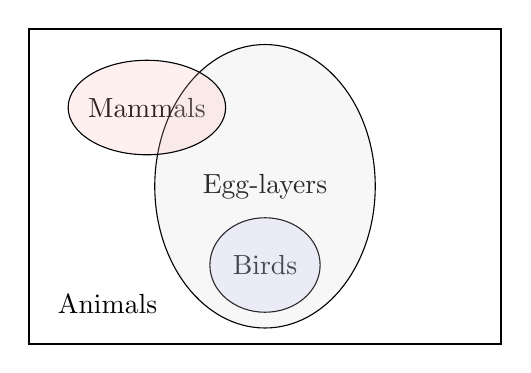
\begin{tikzpicture}
		\draw[thick] (0,0) -- (0,4) -- (6,4) -- (6,0) -- cycle;
		\node (a) at (1,0.5) {Animals};
		\node (e) at (3,2) {Egg-layers};
		\node (b) at (3,1) {Birds};
		\node (m) at (1.5,3) {Mammals};
		\filldraw[fill=blue!30!white, draw =black, fill opacity=0.2] (3,1) ellipse (0.7cm and 0.6cm);
		\filldraw[fill=gray!30!white, draw =black, fill opacity=0.2] (3,2) ellipse (1.4cm and 1.8cm);
		\filldraw[fill=red!30!white, draw =black, fill opacity=0.2] (1.5,3) ellipse (1cm and 0.6cm);
	\end{tikzpicture}
\end{center} In this diagram, the egg-layers are a subset of the animals – not all animals reproduce by laying eggs, so they do not coincide with the whole domain. The birds are a subset of animals too, and in fact wholly within the egg-layers: all birds reproduce oviparously. The mammals are a subset of the animals, and one that overlaps with the egg-layers (the monotremes!), though neither is contained in the other, so the regions overlap without either being wholly within the other. The birds and mammals do not have any common members, so the associated regions do not overlap at all. Note that the sizes of the regions may, but need not, represent the number of things within them. In this diagram they probably don't.

Another example. Consider this interpretation, discussed earlier on page \pageref{poison}: 
		\begin{ekey}
		\item[\text{domain}] people and plants
		\item[C] \gap{1} is a cowboy
		\item[S] \gap{1} sings a sad, sad song
		\item[R] \gap{1} is a rose
		\item[T] \gap{1} has a thorn
	\end{ekey}
The wisdom of Bret Michaels then tells us that the Euler diagram should look like this: \begin{center}
	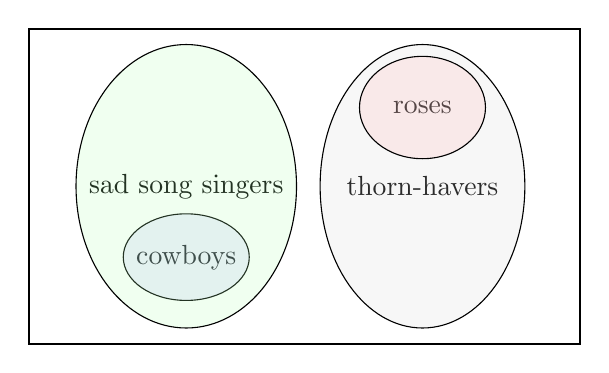
\begin{tikzpicture}
		\draw[thick] (0,0) -- (0,4) -- (7,4) -- (7,0) -- cycle;
		\node (s) at (2,2) {sad song singers};
		\node (t) at (5,2) {thorn-havers};
		\node (c) at (2,1.1) {cowboys};
		\node (r) at (5,3) {roses};
		\filldraw[fill=blue!30!white, draw =black, fill opacity=0.2] (2,1.1) ellipse (0.8cm and 0.55cm);
		\filldraw[fill=green!30!white, draw =black, fill opacity=0.2] (2,2) ellipse (1.4cm and 1.8cm);
		\filldraw[fill=gray!30!white, draw =black, fill opacity=0.2] (5,2) ellipse (1.3cm and 1.8cm);
		\filldraw[fill=red!30!white, draw =black, fill opacity=0.2] (5,3) ellipse (0.8cm and 0.65cm);
	\end{tikzpicture}
\end{center}

If you would like a real challenge, you might try to figure out the interpretation of this Euler diagram from xkcd (`Chat Systems', \url{https://xkcd.com/1810/}):
\begin{center}
	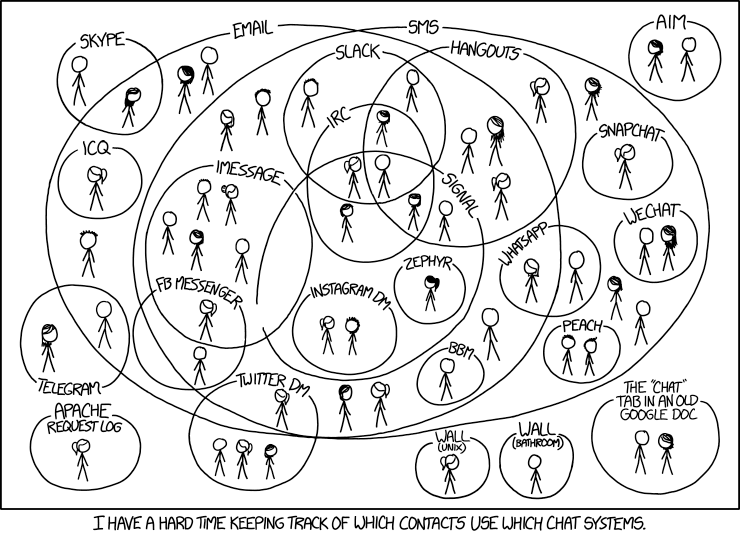
\includegraphics[width=0.85\textwidth]{chat_systems.png}
\end{center}

\paragraph{Representing Two-Place Predicates: Directed Graphs}

Suppose we want to consider just a single two-place predicate, `$R$'. Then we can represent it, in some cases, by depicting the members of the domain by writing them down, and drawing a single-headed arrow between items just in case the relation holds between them (in the right order). Such a diagram is known as a \define{directed graph}, which is given by a collection of \emph{nodes} (the objects in the domain we are representing) and a collection of arrows between them (which represent how the relation holds on that domain.) We stipulate that `$R$' is to hold of \meta{x} and \meta{y} just in case there is an arrow running from \meta{x} to \meta{y} in our diagram. As an example, consider the following interpretation, written in the more standard manner:
\begin{ekey}
	\item[\text{domain}] $1, 2, 3, 4$
	\item[R] \ntuple{1, 2}, \ntuple{2, 3}, \ntuple{3, 4}, \ntuple{4, 1}, \ntuple{1, 3}.
\end{ekey}
That is, an interpretation whose domain is the first four positive whole numbers, and which interprets `$R$' as being true of and only of the specified pairs of numbers. This might be represented by the following simple graph:
\begin{center}
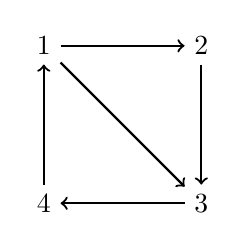
\begin{tikzpicture}
\node (atom1) at (0,2) {1};
\node (atom2) at (2,2) {2};
\node (atom3) at (2,0) {3};
\node (atom4) at (0,0) {4};
\draw[->, thick] (atom1)--(atom2);
\draw[->, thick] (atom2)--(atom3);
\draw[->, thick] (atom3)--(atom4);
\draw[->, thick] (atom4)--(atom1);
\draw[->, thick] (atom1) -- (atom3);
\end{tikzpicture}
\end{center}

Another example; consider the following interpretation: \begin{ekey}
	\item[\text{domain}] $1, 2, 3, 4$
	\item[R] \ntuple{1, 3}, \ntuple{3, 1}, \ntuple{3, 4}, \ntuple{1, 1},\ntuple{3, 3}.
\end{ekey} We might offer this graph to represent it:
\begin{center}
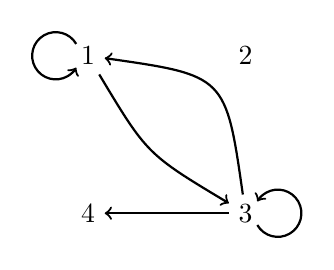
\begin{tikzpicture}
\node (atom1) at (0,2) {1};
\node (atom2) at (2,2) {2};
\node (atom3) at (2,0) {3};
\node (atom4) at (0,0) {4};
\draw[->, thick] (atom3)--(atom4);
\draw[->, thick] (atom1)+(-0.15,0.15) arc (-330:-30:.3); 
\draw[->, thick] (atom3)+(0.15,-0.15) arc (-150:150:.3); 
\draw[->, thick] (atom1) .. controls (0.75,0.75) .. (atom3);
\draw[->, thick] (atom3) .. controls (1.75,1.75) .. (atom1);
\end{tikzpicture}
\end{center} Notice that 2 is in the domain, and hence included as a node in the graph, but it has no arrows attached to it, because it is not included in the relation assigned to $R$. 


If we wanted, we could make our diagrams more complex. For example, we could introduce another kind of arrow to represent an additional two-place relation. Or, we could add names as labels attached to particular objects. Or, to symbolise the extension of a one-place predicate, we might simply draw a ring around some particular objects and stipulate that the thus encircled objects (and only them) are to fall under the predicate `$H$', say.  

Consider how we we might graphically represent the following interpretation, which will make use of all these graphical innovations: \begin{ekey}
	\item[\text{domain}] $2,3,4,5,6$
	\item[G] $\gap{1} \geqslant 4$. 
	\item[D] \gap{1} is distinct from and exactly divisible by \gap{2};
	\item[T] $\gap{1} + 3 = \gap{2}$;
	\item[f] $4$;
\end{ekey} 
This graph represents that interpretation, where the label `$f$' represents the name attached to 4, the blue dotted arrow represents the relation assigned to $T$, the black solid arrow represents the relation assigned to $D$, and the grey ellipse represents the collection of things in the domain which have the property assigned to $G$:
\begin{center}
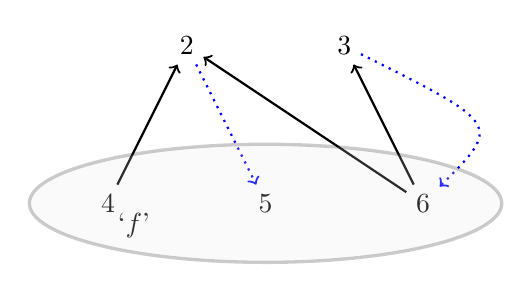
\begin{tikzpicture}
\node (atom2) at (1,2) {2};
\node (atom3) at (3,2) {3};
\coordinate[label=below right:`$f$'] (atom4) at (0,0);
\node (atom4) at (0,0) {4};
\node (atom5) at (2,0) {5};
\node (atom6) at (4,0) {6};
\draw[->, thick] (atom6) -- (atom2);
\draw[->, thick] (atom6) -- (atom3);
\draw[->, thick] (atom4) -- (atom2);
\draw[->, blue, thick, dotted] (atom2) -- (atom5);
\draw[->, blue, thick, dotted] (atom3) .. controls (5,1) .. (atom6);
\filldraw[fill=gray!20!white, draw =black, very thick, opacity=0.2] (2,0) ellipse (3cm and 0.75cm);
\end{tikzpicture}
\end{center}




\keyideas{
	\item An interpretation of \FOL\ is a temporary assignment of extensions to some of the non-logical vocabulary of \FOL\, i.e., the names and predicates of the language.
	\item The extension of a name is a thing from some specified domain.
	\item The extension of an $n$-place predicate is a collection of ordered sequences of length $n$ of things from the domain. The identity predicate has a privileged extension; it is always the collection of pairs from the domain consisting of things and themselves.
	\item The extension of a $0$-place predicate is a truth value; these correspond to atomic sentences of \TFL. 
	\item Given a domain, it is often possible to represent the interpretation of a predicate by means of an Euler diagram or a directed graph on that domain.
}


\practiceproblems
\problempart
Since \FOL\ is an extensional language, if let the \FOL\ name `$s$' denote Superman, and the name `$c$' denote Clark Kent, then `$s=c$' will be true. But it will be true for the same reason that `$s=s$' is true: because \ntuple{Clark Kent,Clark Kent} is in the extension of `$=$'. Can you use this observation as the basis for any argument that English is not an extensional language?

\problempart
Using some of the methods introduced in this section, give a graphical representation of the following interpretations. You will need to rely on your general knowledge to prepare these diagrams. \begin{earg}
	\item \begin{ekey}
		\item[\text{domain}] people
		\item[M] \gap{1} is a musician;
		\item[W] \gap{1} is a woman;
		\item[E] \gap{1} is an economist.
	\end{ekey}
	\item \begin{ekey}
\item[\text{domain}] cards in a standard deck
\item[S] \gap{1} is a seven;
\item[F] \gap{1} is a face card;
\item[R] \gap{1} is red;
\item[j] the Jack of Hearts.
	\end{ekey}
	\item \begin{ekey}
		\item[\text{domain}] Australian states
		\item[L] \gap{1} is larger in population than \gap{2};
		\item[V] \gap{1}'s name ends in a vowel;
		\item[a] South Australia;
		\item[q] Queensland.
	\end{ekey}
\end{earg}

\chapter{Truth in \textnormal{\FOL}}\label{s:TruthFOL}
We know what interpretations are. Since, among other things, they tell us which predicates are true of which objects, they will provide us with an account of the truth of atomic sentences. But we must also present a detailed account of what it is for an arbitrary \FOL\ sentence to be true or false in an interpretation. 

We know from §\ref{s:FOLSentences} that there are three kinds of sentence in \FOL: 
	\begin{itemize}
		\item atomic sentences (i.e., atomic formulae of \FOL\ which have no free variables);
		\item sentences whose main connective is a sentential connective; and
		\item sentences whose main connective is a quantifier.
	\end{itemize}
We need to explain truth for all three kinds of sentence.

I shall offer a completely general explanation in this section. However, to try to keep the explanation comprehensible, I shall at several points use the following interpretation:
	\begin{ekey}
		\item[\text{domain}] all people born before 2000\textsc{ce}
		\item[a] Aristotle
		\item[b] Bush
		\item[W] \gap{1} is wise
		\item[R] \gap{1} was born before \gap{2}
	\end{ekey}
This will be my \emph{go-to example} in what follows.

\section{Atomic sentences}\label{fol.truth.atom}
The truth of atomic sentences should be fairly straightforward. The sentence `$Wa$' should be true just in case `$W$' is true of `$a$'. Given our go-to interpretation, this is true iff Aristotle is wise. Aristotle is wise. So the sentence is true. Equally, `$Wb$' is false on our go-to interpretation.

Likewise, on this interpretation, `$Rab$' is true iff the object named by `$a$' was born before the object named by `$b$'. Well, Aristotle was born before Bush. So `$Rab$' is true. Equally, `$Raa$' is false: Aristotle was not born before Aristotle. 

Dealing with atomic sentences, then, is very intuitive. When $\meta{R}$ is an $n$-place predicate and $\meta{a}_{1}, \meta{a}_{2}, …, \meta{a}_{n}$ are names (not necessarily all different from each other), 

	\factoidbox{
		$\meta{R}\meta{a}_{1}\meta{a}_{2}…\meta{a}_{n}$ is true in an interpretation \textbf{iff}\\
		the objects assigned as the extensions of $\meta{a}_{1}, \meta{a}_{2}, …, \meta{a}_{n}$ in that interpretation (considered in that order) are in the extension assigned to $\meta{R}$ in that interpretation.
	} 

Two other kinds of atomic sentences exist: zero-place predicates, and identity sentences.

\begin{itemize}
	\item A $0$-place predicate is true in an interpretation iff it is assigned the extension true in that interpretation.

	Here in fact, we are using \TFL\ valuations as constituents of \FOL\ interpretations. (A valuation is what you get when you are only intepreting zero-place predicates; we will want it to turn out that the part of \FOL\ which deals just with $0$-place predicates and their truth-functional combinations is the familiar language \TFL, so those interpretations will have to behave like the valuations we are familiar with.)
		\item Identity sentences (two names flanking the identity predicate) are also easy to handle. Where \meta{a} and \meta{b} are any names, 
	\factoidbox{
		$\meta{a} = \meta{b}$ is true in an interpretation \textbf{iff}\\
		 \meta{a} and \meta{b} have the same extension (are assigned the very same object) in that interpretation.}
So in our go-to interpretation, `$a = b$' is false, since Aristotle is distinct from Bush; but `$a=a$' is true.
\end{itemize}






\section{Sentential connectives}\label{fol.truth.sent}
We saw in §\ref{s:FOLSentences} that \FOL\ sentences can be built up from simpler ones using the truth-functional connectives that were familiar from \TFL. The rules governing these truth-functional connectives are \emph{exactly} the same as they were when we considered \TFL. Here they are:
	\factoidbox{Where \meta{A} and \meta{B} are any sentences of \FOL, \begin{itemize}
		\item 
		$\meta{A} \eand \meta{B}$ is true in an interpretation \textbf{iff}\\ both $\meta{A}$ is true and $\meta{B}$ is true in that interpretation
		\item 	$\meta{A} \eor \meta{B}$ is true in an interpretation \textbf{iff}\\ either $\meta{A}$ is true or $\meta{B}$ is true in that interpretation
\item 	$\enot \meta{A}$ is true in an interpretation \textbf{iff} \\$\meta{A}$ is false in that interpretation
\item $\meta{A} \eif \meta{B}$ is true in an interpretation \textbf{iff}\\ either $\meta{A}$ is false or $\meta{B}$ is true in that interpretation
\item $\meta{A} \eiff \meta{B}$ is true in an interpretation \textbf{iff} \\$\meta{A}$ has the same truth value as $\meta{B}$ in that interpretation
	\end{itemize}}
This presents the very same information as the schematic truth tables for the connectives; it just does it in a slightly different way. Some examples will probably help to illustrate the idea. On our go-to interpretation:
	\begin{itemize}
		\item `$a = a \eand Wa$' is true
		\item `$Rab \eand Wb$' is false because, although `$Rab$' is true, `$Wb$' is false
		\item `$a = b \eor Wa$' is true
		\item `$\enot a = b$' is true
		\item `$Wa \eand \enot( a= b \eand Rab)$' is true, because `$Wa$' is true and `$a = b$' is false
	\end{itemize}
Make sure you understand these examples.

\section{When the main connective is a quantifier}\label{fol.truth.quant}
The exciting innovation in \FOL, though, is the use of \emph{quantifiers}. And in fact, expressing the truth conditions for quantified sentences is a bit more fiddly than one might expect. 

Here is a naïve first thought. We want to say that `$\forall x Fx$' is true iff `$F$' is true of everything in the domain. This should not be too problematic: our interpretation will specify directly what `$F$' is true of. 

Unfortunately, this naïve first thought is not general enough. For example, we want to be able to say that `$\forall x \exists y Lxy$' is true just in case `$\exists y Lxy$' is true of everything in the domain. And this is problematic, since our interpretation does not directly specify what `$\exists y Lxy$' is to be true of. Instead, whether or not this is true of something should follow just from the interpretation of `$L$', the domain, and the meanings of the quantifiers. 

So here is a naïve second thought. We might try to say that `$\forall x \exists y Lxy$' is to be true in an interpretation iff $\exists y L\meta{a}y$ is true for \emph{every} name \meta{a} that we have included in our interpretation. And similarly, we might try to say that $\exists y L\meta{a}y$ is true just in case $L\meta{a}\meta{b}$ is true for \emph{some} name \meta{b} that we have included in our interpretation.

Unfortunately, this is not right either. To see this, observe that in our go-to interpretation, we have only given interpretations for \emph{two} names, `$a$' and `$b$'. But the domain – all people born before the year 2000\textsc{ce} – contains many more than two people. I have no intention of trying to name \emph{all} of them!

So here is a third thought. (And this thought is not naïve, but correct.) Although it is not the case that we have named \emph{everyone}, each person \emph{could} have been given a name. So we should focus on this possibility of extending an interpretation, by adding a previously uninterpreted name to our interpretation. I shall offer a few examples of how this might work, centring on our go-to interpretation, and I shall then present the formal definition. 
\begin{itemize}
	\item In our go-to interpretation, `$\exists x Rbx$' should be true. After all, in the domain, there is certainly someone who was born after Bush. Lady Gaga is one of those people. Indeed, if we were to extend our go-to interpretation – temporarily, mind – by adding the name `$c$' to refer to Lady Gaga, then `$Rbc$' would be true on this extended interpretation. And this, surely, should suffice to make `$\exists x Rbx$' true on the original go-to interpretation. 
	\item In our go-to interpretation, `$\exists x (Wx \eand Rxa)$' should also be true. After all, in the domain, there is certainly someone who was both wise and born before Aristotle. Socrates is one such person. Indeed, if we were to extend our go-to interpretation by letting a previously uninterpreted name, `$c$', denote Socrates, then `$Wc \eand Rca$' would be true on this extended interpretation. Again, this should surely suffice to make `$\exists x (Wx \eand Rxa)$' true on the original go-to interpretation. 
	\item In our go-to interpretation, `$\forall x \exists y Rxy$' should be false. After all, consider the last person born in the year 1999. I don't know who that was, but if we were to extend our go-to interpretation by letting a previously uninterpreted name, `$d$', denote that person, then we would not be able to find anyone else in the domain to denote with some further previously uninterpreted name, perhaps `$e$', in such a way that `$Rde$' would be true. Indeed, no matter \emph{whom} we named with `$e$', `$Rde$' would be false. And this observation is surely sufficient to make `$\exists y Rdy$' \emph{false} in our extended interpretation. And this is sufficient to make `$\forall x \exists y Rxy$' false on the original interpretation.
\end{itemize}

If you have understood these three examples, then that's what matters. Strictly speaking, though, we still need to give a precise definition of the truth conditions for quantified sentences. The result, sadly, is a bit ugly, and requires a few new definitions. Brace yourself!

Suppose that \meta{A} is a formula, $\meta{x}$ is a variable, and $\meta{c}$ is a name. We shall write `$\meta{A}\subs{\meta{c}}{\meta{x}}$' to represent the formula that results from replacing or \define{substituting} every free occurrence of $\meta{x}$ in \meta{A} by \meta{c}. So if we began with the formula `$Fxy$', the metalanguage expression ``{`$Fxy$'}$\subs{c}{x}$'' denotes the formula `$Fcy$'. If we began with `$Fyy$', then `$Fyy$'$\subs{c}{x}$ just is the original formula `$Fyy$', since there are no instances of `$x$' in `$Fyy$' to be replaced. If we began with `$Fx \eor \forall x Gx$', then `$Fx \eor \forall x Gx$'$\subs{c}{x}$ is `$Fc \eor \forall x Gx$', since neither occurrence of `$x$' in `$\forall x Gx$' is free.

Suppose we begin with a quantified formula, $\forall \meta{x}\meta{A}$ or $\exists \meta{x}\meta{A}$. If we strip off the quantifier, and pick any name $\meta{c}$, then $\meta{A}\subs{\meta{c}}{\meta{x}}$ is known as a  \define{substitution instance} of the original quantified formulae, and $\meta{c}$ may be called the \define{instantiating name}. So:
	$$\exists x (Rex \eiff Fx)$$
is a substitution instance of 
	$$\forall y \exists x (Ryx \eiff Fx)$$
with the instantiating name `$e$', because  `$\exists x (Ryx \eiff Fx)$'$\subs{e}{y}$ turns out to be `$\exists x (Rex \eiff Fx)$'.

Armed with this notation, the rough idea is as follows. The sentence $\forall \meta{x}\meta{A}$ will be true iff $\meta{A}\subs{\meta{c}}{\meta{x}}$ is true no matter what object (in the domain) we name with $\meta{c}$. Similarly, the sentence $\exists \meta{x}\meta{A}$ will be true iff there is \emph{some} way to assign the name $\meta{c}$ to an object that makes $\meta{A}\subs{\meta{c}}{\meta{x}}$ true. More precisely, we stipulate:\label{quant.tcs.precise}
	\factoidbox{\begin{itemize}
		\item 		$\forall \meta{x}\meta{A}$ is true in an interpretation \textbf{iff}\\ 
		$\meta{A}\subs{\meta{c}}{\meta{x}}$ is true in \emph{every} interpretation that extends the original interpretation by assigning an object to some previously uninterpreted name $\meta{c}$ not appearing in $\meta{A}$ (without changing the original interpretation in any other way).
\item		$\exists \meta{x}\meta{A}$ is true in an interpretation \textbf{iff}\\
		$\meta{A}\subs{\meta{c}}{\meta{x}}$ is true in \emph{some} interpretation that extends the original interpretation by assigning an object to some previously uninterpreted name $\meta{c}$ not appearing in $\meta{A}$ (without changing the original interpretation in any other way).
	\end{itemize}}
That is: we pick a previously uninterpreted name that doesn't appear in \meta{A}.\footnote{There will always be such a previously uninterpreted name: any given sentence of \FOL\ only contains finitely many names, but \FOL\ has a potentially infinite stock of names to draw from.} We uniformly replace any \emph{free} occurrences of the variable \meta{x} in \meta{A} by our previously uninterpreted name, which creates a substitution instance of `$\forall \meta{x}\meta{A}$' and `$\exists \meta{x}\meta{A}$'. Then if this substitution instance is true on every (respectively, some) way of adding an interpretation of the previously uninterpreted name to our existing interpretation, then `$\forall \meta{x}\meta{A}$' (respectively, `$\exists \meta{x}\meta{A}$') is true on that existing interpretation. 

To be clear: all this is doing is formalising (very pedantically) the intuitive idea expressed above. The result is a bit ugly, and the final definition might look a bit opaque. Hopefully, though, the \emph{spirit} of the idea is clear. 

\section{Satisfaction} % Æ introduced this

The discussion of truth in §§\ref{fol.truth.atom}–\ref{fol.truth.quant} only ever involved assigning truth values to sentences. When confronted with formulae involving free variables, we altered them by substituting a previously uninterpreted name for the variable, converting it into a sentence, and temporarily extending the interpretation to cover that previously uninterpreted name. This is a significant departure from the definition of truth for \TFL\ sentences in §\ref{s:SchematicTruthTables}. There, we showed how the truth value of a complex \TFL\ sentence in a valuation depended on the truth value of its constituents in that same valuation. By contrast, on the approach just outlined, the truth value of `$\exists x Fx$' in an interpretation depends on the truth value of some other sentence `$Fc$', which is not a constituent of `$\exists x Fx$', in some different (although related) interpretation! 

There is another way to proceed, which allows arbitrary formulae of \FOL, even those with free variables, to be assigned (temporarily) a truth value. This approach can let the truth value of `$\exists x Fx$' in an interpretation depend on the temporary truth value of `$Fx$' in that same interpretation. This is conceptually  neater than the approach just introduced, and I present it briefly here as an alternative to the substitutional approach of the preceding sections.

\begin{itemize}
 	\item \emph{This section should be regarded as optional, and only for the dedicated student of logic.}
 \end{itemize} 

The inspiration for the approach comes, once again, from thinking of variables in \FOL\ as behaving like pronouns in English. In §\ref{quant.pron} we gave a gloss of `Someone is angry' as `Some person is such that: they are angry'. Concentrate on `they are angry'. This sentence featuring a bare pronoun doesn't express any specific claim intrinsically. But we can, temporarily, fix a referent for the pronoun `they' – temporarily elevating it to the status of a name. If we do so, the sentence can be evaluated. We can introduce a referent by pointing: `They [points to someone] are angry'. Or we can fix a referent by simply assigning one: `Consider that person over there. They are angry'. If we can find someone or other to temporarily be the referent of the pronoun `they', then it will be true that there is someone such that they are angry. If no matter who we fix as the referent, they are angry, then it will be true that everyone is such that they are angry. 

This is, in a nutshell, the idea we will use to handle quantification in \FOL. Let us introduce some terminology: \factoidbox{
	A \define{variable assignment} over an interpretation is an assignment of exactly one object from the domain of that interpretation to each variable that we care to consider.
}  
If we have an interpretation, and a variable assignment, then we can evaluate every formula of \FOL\ – not only sentences. Of course, the evaluation of the open formulae will be very fragile, since even given a single background interpretation, a formula like `$Fx$' might be true relative to one variable assignment and false relative to another. 

Let us start, as before, by giving rules for evaluating atomic formulae of \FOL, given an interpretation and a variable assignment. \factoidbox{Where $\meta{R}$ is any $n$-place predicate ($n ≥ 0$), and $\meta{t}_{1},…,t_{n}$ are any terms – variables or names, then: \begin{itemize}
	\item  $\meta{R}\meta{t}_{1}…\meta{t}_{n}$ is true on a variable assignment over an interpretation \textbf{iff}\\
	$\meta{R}$ is true of the objects assigned to the terms $\meta{t}_{1},…,\meta{t}_{n}$  by that variable assignment and that intepretation, considered in that order.
	\item $\meta{t}_{1}=\meta{t}_{2}$ is true on a variable assignment over an interpretation \textbf{iff}\\
	$\meta{t}_{1}$ and $\meta{t}_{2}$ are assigned the very same object by that variable assignment in that interpretation.
\end{itemize}} These are very similar clauses to those we saw for atomic sentences in §\ref{fol.truth.quant}. Indeed, when we are considering atomic sentences of \FOL, the mention of a variable assignment is redundant, since no atomic sentence contains a variable. (If an atomic formula contains a variable, the variable would be free and the formula thus not a sentence.)

The recursion clauses that extend truth for atomic formulae to truth for arbitrary formulae are these (I omit the clauses for $\eor$, $\eif$, and $\eiff$, which you can easily fill in yourself, following the model in §\ref{fol.truth.sent}): \factoidbox{Where \meta{A} and \meta{B} are formulae of \FOL, and \meta{x} is a variable:
	\begin{itemize}
		\item $\enot \meta{A}$ is true on a variable assignment over an interpretation \textbf{iff}\\
		\meta{A} is false on that variable assignment over that interpretation;
		\item $\meta{A} \eand \meta{B}$ is true on a variable assignment over an interpretation \textbf{iff}\\
		both \meta{A} is true on that variable assignment over that interpretation and \meta{B} is true on that variable assignment over that interpretation;
		\item …
		\item $\forall \meta{x}\meta{A}$ is is true on a variable assignment over an interpretation \textbf{iff}\\
		\meta{A} is true on \emph{every} variable assignment differing from the original one at most in what it assigns to \meta{x} over that interpretation;
		\item $\exists \meta{x}\meta{A}$ is is true on a variable assignment over an interpretation \textbf{iff}\\
		\meta{A} is true on \emph{some} variable assignment differing from the original one at most in what it assigns to \meta{x} over that interpretation.
	\end{itemize}
}

The last two clauses are where this approach is strongest. Rather than considering some substitition instance of $\forall\meta{x}\meta{A}$, we simply consider the direct constituent \meta{A}. Rather than considering all variations on the original interpretation which include some previously uninterpreted name, we simply consider all ways of varying what is assigned to \meta{x} by the original variable assignment, but keeping everything else unchanged. If you see the rationale for the clauses offered in §\ref{fol.truth.quant}, you can see why the clauses just offered are appropriate.

We now have the idea of truth on a variable assignment over an intepretation. But what we want – if this alternative approach is to yield the same end result – is truth in an interpretation. Notice that, given an interpretation, varying the variable assignment can change the truth value of a formula with free variables. But it cannot change the truth value of a formula which is a sentence, so if a sentence is true on one variable assignment over an interpretation, it is true on every variable assignment over that interpretation. So we can reintroduce the notion of truth in an intepretation, like so: \factoidbox{
	 \meta{A} is true in an interpretation \textbf{iff}\\
	 \meta{A} is a sentence of \FOL, and \meta{A} is true on any (or every) variable assignment over that interpretation.
} 

Here's how this works in practice. Suppose we want to figure out whether the sentence `$\forall x \exists y Lxy$' is true on an interpretation which  associates the two-place predicate `$L$' with the relation `\gap{1} is no heavier than \gap{2}', and has as its domain the planets in our solar system. We might reason as follows: \begin{quote}
	\emph{For each way of picking planets to be the values of `$x$' and `$y$', either we pick two different planets, and one is lighter than the other (no two planets have the same mass); or we pick the same planet, and `they' are identical in mass. In either case, we can always find something no heavier than anything we pick. So for any variable assignment to `$x$' over this interpretation,  we can then assign something to `$y$' so as to make `$Lxy$' true on that joint assignment. Hence no matter what we assign to `$x$', `$\exists y Lxy$' is true on that assignment. But since that is true no matter what we assign to `$x$', `$\forall x \exists y Lxy$' is true on every variable assignment over this interpretation. But that latter is a sentence, so is true in this interpretation.}
\end{quote}

Let us say that a sequence of objects \ntuple{$a_{1},…,a_{n}$} \define{satisfies} a formula $\meta{A}$ in which the variables $\meta{x}_{1},…,\meta{x}_{n}$ occur freely iff there is a variable assignment over an intepretation whose domain includes each $a_{i}$, and which assigns each $a_{i}$ to the variable $\meta{x}_{i}$, and on which \meta{A} is true over that interpretation. What we have expressed in terms of variable assignments could have been expressed, a little more awkwardly, using the notion of some objects satisfying a formula. Indeed, this is how Alfred Tarski, the inventor of this approach to truth in \FOL, first introduced the idea.\footnote{A translation of his original 1933 paper is `The Concept of Truth in Formalized Languages', 1983, in Tarski, \emph{Logic, Semantics, Metamathematics}, Indianapolis: Hackett, pp. 152–278. It is rather technical in places.}

\keyideas{
	\item An atomic sentence  of \FOL\ is true in an interpretation iff the extensions of the names occurring in it, taken in the appropriate order, fall in the extension of the predicate they accompany.
	\item A compound sentence  of \FOL\ has truth conditions relative to an interpretation that are the same as those for \TFL, if the main connective is truth-functional.
	\item A compound sentence of \FOL\ whose main connective is a quantifier `$\forall x$' (resp., `$\exists x$') is true in an interpretation if on every (resp., some) interpretation extending the first by assigning an extension to some previously uninterpreted name `$c$', the result of replacing every occurence of the variable `$x$' bound by the quantifier with $c$ is true.
}

\practiceproblems


\problempart
\label{pr.TorF1}
Consider the following interpretation:
	\begin{ekey}
		\item[\text{domain}] The domain comprises only Corwin and Benedict
		\item[A] is to be true of both Corwin and Benedict
		\item[B] is to be true of Benedict only
		\item[N] is to be true of no one
		\item[c] is to refer to Corwin
	\end{ekey}
Determine whether each of the following sentences is true or false in that interpretation:
\begin{earg}
\item $Bc$
\item $Ac \eiff \enot Nc$
\item $Nc \eif (Ac \eor Bc)$
\item $\forall x Ax$
\item $\forall x \enot Bx$
\item $\exists x(Ax \eand Bx)$
\item $\exists x(Ax \eif Nx)$
\item $\forall x(Nx \eor \enot Nx)$
\item $\exists x Bx \eif \forall x Ax$
\end{earg}

\problempart
\label{pr.TorF3}
Consider the following interpretation:	
	\begin{ekey}
		\item[\text{domain}] The domain comprises only Lemmy, Courtney and Eddy
		\item[G] is to be true of Lemmy, Courtney and Eddy.
		\item[H] is to be true of and only of Courtney
		\item[M] is to be true of and only of Lemmy and Eddy
		\item[c] is to refer to Courtney
		\item[e] is to refer to Eddy
	\end{ekey}
Determine whether each of the following sentences is true or false in that interpretation:
\begin{earg}
\item $Hc$
\item $He$
\item $Mc \eor Me$
\item $Gc \eor \enot Gc$
\item $Mc \eif Gc$
\item $\exists x Hx$
\item $\forall x Hx$
\item $\exists x \enot Mx$
\item $\exists x(Hx \eand Gx)$
\item $\exists x(Mx \eand Gx)$
\item $\forall x(Hx \eor Mx)$
\item $\exists x Hx \eand \exists x Mx$
\item $\forall x(Hx \eiff \enot Mx)$
\item $\exists x Gx \eand \exists x \enot Gx$
\item $\forall x\exists y(Gx \eand Hy)$
\end{earg}

\problempart
% \label{pr.TorF3}
Following the diagram conventions introduced at the end of §\ref{s:Interpretations}, consider the following interpretation:	
\begin{center}
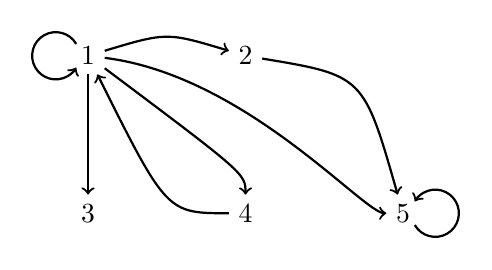
\begin{tikzpicture}
\node (atom1) at (0,2) {1};
\node (atom2) at (2,2) {2};
\node (atom4) at (0,0) {3};
\node (atom5) at (2,0) {4};
\node (atom6) at (4,0) {5};
\draw[->, thick] (atom1)+(-0.15,0.15) arc (-330:-30:.3); 
\draw[->, thick] (atom6)+(0.15,-0.15) arc (-150:150:.3); 
\draw[->, thick] (atom1) .. controls (1,2.3) .. (atom2);
\draw[->, thick] (atom1) -- (atom4);
\draw[->, thick] (atom5) .. controls (1,0) .. (atom1);
\draw[->, thick] (atom1) .. controls (2,0.5) .. (atom5);
\draw[->, thick] (atom1) .. controls (2,1.75) and (3.5,0) .. (atom6);
\draw[->, thick] (atom2) .. controls (3.5,1.75) .. (atom6);
\end{tikzpicture}
\end{center}
Determine whether each of the following sentences is true or false in that interpretation:
\begin{earg}
\item $\exists x Rxx$
\item $\forall x Rxx$
\item $\exists x \forall y Rxy$
\item $\exists x \forall y Ryx$
\item $\forall x \forall y \forall z ((Rxy \eand Ryz) \eif Rxz)$
\item $\forall x \forall y \forall z ((Rxy \eand Rxz) \eif Ryz)$
\item $\exists x \forall y \enot Rxy$
\item $\forall x(\exists y Rxy \eif \exists y Ryx)$
\item $\exists x \exists y (\enot x = y \eand Rxy \eand Ryx)$
\item $\exists x \forall y(Rxy \eiff x = y)$
\item $\exists x \forall y(Ryx \eiff x = y)$
\item $\exists x \exists y(\enot x = y \eand Rxy \eand \forall z(Rzx \eiff y = z))$
\end{earg}

\problempart
Why, when we are trying to figure out whether `$\forall x Rxa$' is true in an interpretation, do we need to consider whether `$Rca$' is true in some expanded interpretation with a \emph{new} name `$c$'. Why can't we make do with substituting a name we've already interpreted?

\problempart
Explain why on page \pageref{quant.tcs.precise} we did not give the truth conditions for the existential quantifer like this: \begin{quote}
	$\exists\meta{x}\meta{A}\subs{x}{c}$ is true in an interpretation $I$ iff in \emph{some} interpretation just like $I$ except that might assign something different to \meta{c}, $\meta{A}$ is true.
\end{quote}






\chapter{Semantic concepts}\label{FOL.semantics}
Offering a precise definition of truth in \FOL\ was more than a little fiddly. But now that we are done, we can define various central logical notions. These will look very similar to the definitions we offered for \TFL. However, remember that they concern \emph{interpretations}, rather than valuations. 


We will use the symbol `$\entails$' for entailment in \FOL, much as we did for \TFL. This introduces an ambiguity, but a harmless one, since every valid argument in \TFL\ remains a valid argument in \FOL.

So:\factoidbox{\begin{itemize}
	\item  	$\meta{A}_1, \meta{A}_2, …, \meta{A}_n$ together \define{entail} \meta{C} (written $\meta{A}_1, \meta{A}_2, …, \meta{A}_n \entails\meta{C}$) iff there is no interpretation in which all of $\meta{A}_1, \meta{A}_2, …, \meta{A}_n$ are true and in which \meta{C} is false.
	\item An \FOL\ sentence $\meta{A}$ is a \define{logical truth} iff $\meta{A}$ is true in every interpretation; this is written  $\entails\meta{A}$.
	\item $\meta{A}$ is a \define{contradiction} iff $\meta{A}$ is false in every interpretation; i.e., $\entails\enot\meta{A}$.

\item Two \FOL\ sentences \meta{A} and \meta{B} are \define{logically equivalent} iff they are true in exactly the same interpretations as each other; i.e., both $\meta{A}\entails\meta{B}$ and $\meta{B}\entails\meta{A}$.
\item The \FOL\ sentences $\meta{A}_1,\meta{A}_2,…, \meta{A}_n$ are \define{jointly consistent} iff there is some interpretation in which all of the sentences are true. They are \define{jointly inconsistent} iff there is no such interpretation.\end{itemize}}

As before, there is a close connection between validity and entailment: \factoidbox{
 $\meta{A}_1, \meta{A}_2, … \meta{A}_n \ttherefore \meta{C}$ is \define{valid} in \FOL\ iff there is no interpretation in which all of the premises are true and the conclusion is false; i.e., $\meta{A}_1,\meta{A}_2,… \meta{A}_n \entails\meta{C}$. It is \define{invalid} in \FOL\ otherwise.} Our entailments are conclusive in virtue of form, because the consideration of many alternative interpretations of the non-logical expressions involved means that no argument can be conclusive because of some special `connection in meaning' between such expressions in the language. Entailment in \FOL\ reflects only the logical structure of the sentences involved, where this now includes the new logical resources of \FOL\ over \TFL.

\section{Some subtleties about truth and interpretation} % Æ added

Our interpretations allow us a precise characterisation of formal truth for \FOL. In §\ref{s:Valid}, we introduced the idea of the structure of a sentence, and the pragmatic approach that logicians take to that notion. In \FOL, the logical constants are those of \TFL\ plus the quantifiers and the identity predicate. But every other item of the language is up for reinterpretation, and our interpretations allow us to reinterpret these expressions in an arbitrary fashion.

In \TFL, we were able to characterise a logical truth as a sentence which is actually true on every reinterpretation of non-logical expressions (in \TFL, the non-logical expressions are just are the atomic sentences). And we characterised a formally valid argument as one in which each possible reinterpretation (i.e., valuation) of the  premises which makes them actually true, is also one which makes the conclusion actually true.

But this account of formal validity needs refining when it comes to \FOL. Consider the \FOL\ sentence which says that there are at least three things: $$\exists x \exists y \exists z (x≠y \eand x≠z \eand y≠z).$$ This sentence contains no non-logical expressions. Hence the sentence has a constant meaning, and is true on each reinterpretation just in case it is actually true. It is actually true – there are actually at least three things. Hence our \TFL-inspired account of logical truth would suggest that this sentence is a logical truth. But it seems very strange to think that it is a truth of logic alone that there are at least three things. Isn't it possible that there had been fewer?

The keen-eyed among you will have noticed that this sentence is not, in fact, a logical truth of \FOL. The reason is that in defining truth for sentences of \FOL, we considered not just reinterpretations of the non-logical expressions, but also we allowed the domain of our interpretation to freely depart from actuality. So we are, in effect, allowing our interpretations to vary the meanings of the non-logical vocabulary \emph{and} to vary the possible situations at which our sentences are to be evaluated. So we can consider a possible situation in which there are just two things, and if that situation provides the domain of an interpretation, there is no way of extending that interpretation to three names `$a$', `$b$', and `$c$' such that `$a≠b \eand a≠c \eand b≠c$' is true; hence `$\exists x \exists y \exists z (x≠y \eand x≠z \eand y≠z)$' isn't true on the original interpretation.

One sentence of this class is nevertheless a logical truth: the claim that something exists, `$\exists x x=x$'. Since it is a constraint on \FOL\ domains that they cannot be empty (§\ref{sec_domains}), there is for any interpretation a way of adding a previously uninterpreted name `$c$' which denotes an object in the domain, and of course `$c=c$' is true in that extended interpretation, since each name must have a referent in any interpretation, and the identity predicate is always interepreted as representing pairs of objects in the domain and themselves.

\keyideas{
	\item Definitions of entailment, consistency, contradiction and logical equivalence can be given for \FOL\ that are very close parallels to those for \TFL, though given in terms of intepretations not valuations.
	\item The notion of a logical truth in \FOL\ is slightly different than the notion of a tautology, since we allow interpretations that vary not just in what they assign as extensions to the non-logical vocabulary, but also variation in the domain over which quantifiers range. Nothing like the latter feature occurs in \TFL\ valuations, but it is crucial for ensuring that contingent truths without names or non-logical predicates aren't misclassified as logical truths.
}





\chapter{Demonstrating Consistency and Invalidity}\label{sec.UsingModels}

\section{Logical truths and contradictions}
Suppose we want to show that `$\exists xAxx \eif Bd$' is \emph{not} a logical truth. This requires showing that the sentence is not true in every interpretation; i.e.,\ that it is false in some interpretation. If we can provide just one interpretation in which the sentence is false, then we will have shown that the sentence is not a logical truth.

In order for `$\exists xAxx \eif Bd$' to be false, the antecedent (`$\exists x Axx$') must be true, and the consequent (`$Bd$') must be false. To construct such an interpretation, we start by specifying a domain. Keeping the domain small makes it easier to specify what the predicates will be true of, so we shall start with a domain that has just one member. For concreteness, let's say it is the city of Paris. 
	\begin{ekey}
		\item[\text{domain}] Paris
	\end{ekey}
The name `$d$' must name something in the domain, so we have no option but:
	\begin{ekey}
		\item[d] Paris
	\end{ekey}
Recall that we want `$\exists x Axx$' to be true, so we want all members of the domain to be paired with themselves in the extension of `$A$'. We can offer:
	\begin{ekey}
		\item[A] \gap{1} is in the same place as \gap{2}
	\end{ekey}
Now `$Add$' is true, so it is surely true that `$\exists x Axx$'. Next, we want `$Bd$' to be false, so the referent of `$d$' must not be in the extension of `$B$'. We might simply offer:
	\begin{ekey}
		\item[B] \gap{1} is in Germany
	\end{ekey}
Now we have an interpretation where `$\exists x Axx$' is true, but where `$Bd$' is false. So there is an interpretation where `$\exists x Axx \eif Bd$' is false. So `$\exists x Axx \eif Bd$' is not a logical truth.

We can just as easily show that `$\exists xAxx \eif Bd$' is not a contradiction. We need only specify an interpretation in which `$\exists xAxx \eif Bd$' is true; i.e., an interpretation in which either `$\exists x Axx$' is false or `$Bd$' is true. Here is one:
	\begin{ekey}
		\item[\text{domain}] Paris
		\item[d] Paris
		\item[A] \gap{1} is in the same place as \gap{2}
		\item[B] \gap{1} is in France
	\end{ekey}
This shows that there is an interpretation where `$\exists xAxx \eif Bd$' is true. So `$\exists x Axx \eif Bd$' is not a contradiction.

\section{Logical equivalence}
Suppose we want to show that `$\forall x Sx$' and `$\exists x Sx$' are not logically equivalent. We need to construct an interpretation in which the two sentences have different truth values; we want one of them to be true and the other to be false. We start by specifying a domain. Again, we make the domain small so that we can specify extensions easily. In this case, we shall need at least two objects. (If we chose a domain with only one member, the two sentences would end up with the same truth value. In order to see why, try constructing some partial interpretations with one-member domains.) For concreteness, let's take:
	\begin{ekey}
		\item[\text{domain}] Ornette Coleman, Sarah Vaughan
	\end{ekey}
We can make `$\exists x Sx$' true by including something in the extension of `$S$', and we can make `$\forall x Sx$' false by leaving something out of the extension of `$S$'. For concreteness we shall offer:
	\begin{ekey}
		\item[S] \gap{1} plays saxophone
	\end{ekey}
Now `$\exists x Sx$' is true, because `$S$' is true of Ornette Coleman. Slightly more precisely, extend our interpretation by allowing `$c$' to name Ornette Coleman.  `$Sc$' is true in this extended interpretation, so `$\exists x Sx$' was true in the original interpretation. Similarly, `$\forall x Sx$' is false, because `$S$' is false of Sarah Vaughan. Slightly more precisely, extend our interpretation by allowing `$d$' to name Sarah Vaughan, and `$Sd$' is false in this extended interpretation, so `$\forall x Sx$' was false in the original interpretation. We have provided a counter-interpretation to the claim that `$\forall x Sx$' and `$\exists x Sx$' are logically equivalent.
	\factoidbox{
		To show that $\meta{A}$ is not a logical truth, it suffices to find an interpretation where $\meta{A}$ is false.
		
		To show that $\meta{A}$ is not a contradiction, it suffices to find an interpretation where $\meta{A}$ is true.
		
		To show that $\meta{A}$ and $\meta{B}$ are not logically equivalent, it suffices to find an interpretation where one is true and the other is false.
	}

\section{Validity, entailment and consistency}
To test for validity, entailment, or consistency, we typically need to produce interpretations that determine the truth value of several sentences simultaneously. 

Consider the following argument in \FOL:
$$\exists x(Gx \eif Ga) \ttherefore \exists x Gx \eif Ga$$
To show that this is invalid, we must make the premise true and the conclusion false. The conclusion is a conditional, so to make it false, the antecedent must be true and the consequent must be false. Clearly, our domain must contain two objects. Let's try:
	\begin{ekey}
		\item[\text{domain}] Karl Marx, Ludwig von Mises
		\item[G] \gap{1} hated communism
		\item[a] Karl Marx
	\end{ekey}
Given that Marx wrote \emph{The Communist Manifesto}, `$Ga$' is plainly false in this interpretation. But von Mises famously hated communism. So `$\exists x Gx$' is true in this interpretation. Hence `$\exists x Gx \eif Ga$' is false, as required. 

But does this interpretation make the premise true? Yes it does! For `$\exists x (Gx \eif Ga)$' to be true,  `$Gc \eif Ga$' must be true in  some extended interpretation that is almost exactly like the interpretation just given, except that it also interprets some previously uninterpreted name `$c$'. Let's extend our original interpretation by letting `$c$' denote Karl Marx – the same thing as `$a$' denotes in the original interpretation. Since `$a$' and `$c$' denote the same thing in the extended interpretation, obviously `$Gc \eif Ga$' will be true. So `$\exists x (Gx \eif Ga)$' is true in the original interpretation. So the premise is true, and the conclusion is false, in this original interpretation. The argument is therefore invalid. 

In passing, note that we have also shown that `$\exists x(Gx \eif Ga)$' does \emph{not} entail `$\exists x Gx \eif Ga$'. And equally, we have shown that the sentences `$\exists x (Gx \eif Ga)$' and `$\enot (\exists x Gx \eif Ga)$' are jointly consistent.

Let's consider a second example. Consider:
	$$\forall x \exists y Lxy \ttherefore \exists y \forall x Lxy$$
Again, I want to show that this is invalid. To do this, we must make the premises true and the conclusion false. Here is a suggestion:
	\begin{ekey}
		\item[\text{domain}] People with a living biological sibling
		\item[L] \gap{1} shares a parent with \gap{2}
	\end{ekey}
The premise is clearly true on this interpretation. Anyone in the domain has a living sibling. That sibling will also, then, be in the domain, because one cannot be someone's sibling without also having  them as a sibling. So for everyone in the domain, there will be at least one other person in the domain who is their sibling, and thus has a parent in common with them. Hence `$\forall x \exists y Lxy$' is true. But the conclusion is clearly false, for that would require that there is some single person who shares a parent with everyone in the domain, and there is no such person. So the argument is invalid. We observe immediately that the sentences `$\forall x \exists y Lxy$' and `$\enot\exists y \forall x Lxy$' are jointly consistent and that `$\forall x \exists y Lxy$' does not entail `$\exists y \forall x Lxy$'. 

For my third example, I shall mix things up a bit. In §\ref{s:Interpretations}, I described how we can present some interpretations using diagrams. For example:
\begin{center}
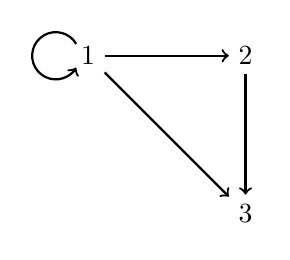
\begin{tikzpicture}
\node (atom1) at (0,2) {1};
\node (atom2) at (2,2) {2};
\node (atom3) at (2,0) {3};
\draw[->, thick] (atom1)--(atom2);
\draw[->, thick] (atom1)--(atom3);
\draw[->, thick] (atom1)+(-0.15,0.15) arc (-330:-30:.3); 
\draw[->, thick] (atom2) -- (atom3);
\end{tikzpicture}
\end{center}
Using the conventions employed in §\ref{s:Interpretations}, the domain of this interpretation is the first three positive whole numbers, and `$R$' is true of \meta{x} and \meta{y} just in case there is an arrow from \meta{x} to \meta{y} in our diagram. Here are some sentences that the interpretation makes true:
	\begin{itemize}
		\item `$\forall x \exists y Ryx$' 
		\item `$\exists x \forall y Rxy$' \hfill witness 1
		\item `$\exists x \forall y (Ryx \eiff x = y)$' \hfill witness 1
		\item `$\exists x \exists y \exists z (\enot y = z \eand Rxy \eand Rzx)$' \hfill witness 2
		\item `$\exists x \forall y \enot Rxy$' \hfill witness 3
		\item `$\exists x (\exists y Ryx \eand \enot \exists y Rxy)$' \hfill witness 3
	\end{itemize}
This immediately shows that all of the preceding six sentences are jointly consistent. We can use this observation to generate \emph{invalid} arguments, e.g.:
	\begin{align*}
		\forall x \exists y Ryx, \exists x \forall y Rxy  &\ttherefore  \forall x \exists y Rxy\\
		\exists x \forall y Rxy, \exists x \forall y \enot Rxy & \ttherefore \enot \exists x \exists y \exists z (\enot y = z \eand Rxy \eand Rzx)
	\end{align*}
and many more besides.

	\factoidbox{
	To show that $\meta{A}_1, \meta{A}_2, …, \meta{A}_n \ttherefore \meta{C}$ is invalid, it suffices to find an interpretation where all of $\meta{A}_1, \meta{A}_2, …, \meta{A}_n$ are true and where $\meta{C}$ is false.
	
	That same interpretation will show that $\meta{A}_1, \meta{A}_2, …, \meta{A}_n$ do not entail $\meta{C}$.
	
	That same interpretation will show that $\meta{A}_1, \meta{A}_2, …, \meta{A}_n, \enot \meta{C}$ are jointly consistent.}
When you provide an interpretation to refute a claim – to logical truth, say, or to entailment – this is sometimes called providing a \emph{counter-interpretation} (or providing a \emph{counter-model}).

\keyideas{
	\item Testing for consistency and invalidity involves displaying just a single appropriate interpretation.
	\item It can be a subtle matter to figure out what such an interpretation might be like. 
	\item An interpretation which shows an argument invalid is a counterexample to that argument. 
}

\practiceproblems

\problempart
The following entailments are correct in \FOL. In each case, explain why.
\begin{earg}
 	\item $\forall x Qx, \forall x (Qx \eif Rx) \entails \exists x Rx$;
 	\item $\forall x\forall y \bigl(Rxy \eif \forall z(Ryz \eif x≠z)\bigr) \entails (Raa \eif \enot Raa)$.
 \end{earg} 

\problempart
\label{pr.Contingent}
Show that each of the following is neither a logical truth nor a contradiction:
\begin{earg}
\item \leftsolutions\ $Da \eand Db$
\item \leftsolutions\ $\exists x Txh$
\item \leftsolutions\ $Pm \eand \enot\forall x Px$
\item $\forall z Jz \eiff \exists y Jy$
\item $\forall x (Wxmn \eor \exists yLxy)$
\item $\exists x (Gx \eif \forall y My)$
\item $\exists x (x = h \eand x = i)$
\end{earg}

\solutions
\problempart
\label{pr.NotEquiv}
Show that the following pairs of sentences are not logically equivalent.
\begin{earg}
\item $Ja$, $Ka$
\item $\exists x Jx$, $Jm$
\item $\forall x Rxx$, $\exists x Rxx$
\item $\exists x Px \eif Qc$, $\exists x (Px \eif Qc)$
\item $\forall x(Px \eif \enot Qx)$, $\exists x(Px \eand \enot Qx)$
\item $\exists x(Px \eand Qx)$, $\exists x(Px \eif Qx)$
\item $\forall x(Px\eif Qx)$, $\forall x(Px \eand Qx)$
\item $\forall x\exists y Rxy$, $\exists x\forall y Rxy$
\item $\forall x\exists y Rxy$, $\forall x\exists y Ryx$
\end{earg}



\problempart
Show that the following sentences are jointly consistent:
\begin{earg}
\item $Ma, \enot Na, Pa, \enot Qa$
\item $Lee, Leg, \enot Lge, \enot Lgg$
\item $\enot (Ma \eand \exists x Ax), Ma \eor Fa, \forall x(Fx \eif Ax)$
\item $Ma \eor Mb, Ma \eif \forall x \enot Mx$
\item $\forall y Gy, \forall x (Gx \eif Hx), \exists y \enot Iy$
\item $\exists x(Bx \eor Ax), \forall x \enot Cx, \forall x\bigl( (Ax \eand Bx) \eif Cx\bigr)$
\item $\exists x Xx, \exists x Yx, \forall x(Xx \eiff \enot Yx)$
\item $\forall x(Px \eor Qx), \exists x\enot(Qx \eand Px)$
\item $\exists z(Nz \eand Ozz), \forall x\forall y(Oxy \eif Oyx)$
\item $\enot \exists x \forall y Rxy, \forall x \exists y Rxy$
\item $\enot Raa$, $\forall x (x=a \eor Rxa)$
\item $\forall x\forall y\forall z(x=y \eor y=z \eor x=z)$, $\exists x\exists y\ \enot x= y$
\item $\exists x\exists y(Zx \eand Zy \eand x=y)$, $\enot Zd$, $d=e$
\end{earg}

\problempart
Show that the following arguments are invalid:
\begin{earg}
\item $\forall x(Ax \eif Bx) \ttherefore \exists x Bx$
\item $\forall x(Rx \eif Dx), \forall x(Rx \eif Fx) \ttherefore \exists x(Dx \eand Fx)$
\item $\exists x(Px\eif Qx) \ttherefore \exists x Px$
\item $Na \eand Nb \eand Nc \ttherefore \forall x Nx$
\item $Rde, \exists x Rxd \ttherefore Red$
\item $\exists x(Ex \eand Fx), \exists x Fx \eif \exists x Gx \ttherefore \exists x(Ex \eand Gx)$
\item $\forall x Oxc, \forall x Ocx \ttherefore \forall x Oxx$
\item $\exists x(Jx \eand Kx), \exists x \enot Kx, \exists x \enot Jx \ttherefore \exists x(\enot Jx \eand \enot Kx)$
\item $Lab \eif \forall x Lxb, \exists x Lxb \ttherefore Lbb$
\item $\forall x(Dx \eif \exists y Tyx) \ttherefore \exists y \exists z\ \enot y= z$
\end{earg}

\chapter{Reasoning about all interpretations: demonstrating inconsistency and validity}\label{s:All.Interp}

\section{Logical truths and contradictions}
We can show that a sentence is \emph{not} a logical truth just by providing one carefully specified interpretation: an interpretation in which the sentence is false. To show that something is a logical truth, on the other hand, it would not be enough to construct ten, one hundred, or even a thousand interpretations in which the sentence is true. A sentence is only a logical truth if it is true in \emph{every} interpretation, and there are infinitely many interpretations. We need to reason about all of them, and we cannot do this by dealing with them one by one!

Sometimes, we can reason about all interpretations fairly easily. For example, we can offer a relatively simple argument that `$Raa\eiff Raa$' is a logical truth:
	\begin{quote}
		\label{allmodels1}
		Any relevant interpretation will give `$Raa$' a truth value. If `$Raa$' is true in an interpretation, then `$Raa \eiff Raa$' is true in that interpretation. If `$Raa$' is false in an interpretation, then `$Raa \eiff Raa$' is true in that interpretation. These are the only alternatives. So `$Raa \eiff Raa$' is true in every interpretation. Therefore, it is a logical truth.
	\end{quote}
This argument is valid, of course, and its conclusion is true. However, it is not an argument in \FOL. Rather, it is an argument in English \emph{about} \FOL: it is an argument in the metalanguage. 

Note another feature of the argument. Since the sentence in question contained no quantifiers, we did not need to think about how to interpret `$a$' and `$R$'; the point was just that, however we interpreted them, `$Raa$' would have some truth value or other. (We could ultimately have given the same argument concerning \TFL\ sentences.)

Here is another bit of reasoning. Consider the sentence `$\forall x(Rxx\eiff Rxx)$'. Again, it should obviously be a logical truth. But to say precisely why is quite a challenge. We cannot say that `$Rxx \eiff Rxx$' is true in every interpretation, since `$Rxx \eiff Rxx$' is not even a \emph{sentence} of \FOL\ (remember that `$x$' is a variable, not a name). So we have to be a bit cleverer. 
	\begin{quote}
		Consider some arbitrary interpretation. Consider some arbitrary member of the model's domain, which, for convenience, we shall call \emph{obbie}, and suppose we extend our original interpretation by adding a previously uninterpreted name, `$c$', to name \emph{obbie}. Then either `$Rcc$' will be true or it will be false. If `$Rcc$' is true, then `$Rcc \eiff Rcc$' is true. If `$Rcc$' is false, then `$Rcc \eiff Rcc$' will be true. So either way, `$Rcc \eiff Rcc$' is true. Since there was nothing special about \emph{obbie} – we might have chosen any object – we see that no matter how we extend our original interpretation by allowing `$c$' to name some new object, `$Rcc \eiff Rcc$' will be true in the new interpretation. So `$\forall x (Rxx \eiff Rxx)$' was true in the original interpretation. But we chose our interpretation arbitrarily. So `$\forall x (Rxx \eiff Rxx)$' is true in every interpretation. It is therefore a logical truth.
	\end{quote}
This is quite longwinded, but, as things stand, there is no alternative. In order to show that a sentence is a logical truth, we must reason about \emph{all} interpretations. 

But sometimes we can draw a conclusion about some way all interpretations must be, by considering a hypothetical interpretation which isn't that way, and showing that hypothesis leads to trouble. Here is an example. \begin{quote}
	Suppose there were an interpretation which makes `$a≠b \eif \enot \exists x(x=a \eand x=b)$' false. Then while `$a≠b$' is true on that interpretation, `$\enot \exists x(x=a \eand x=b)$' must be false. So `$\exists x(x=a \eand x=b)$' must be true; and hence it has some true substitition instance with some previously uninterpreted name `$c$' as the instantiating name: `$c=a \eand c=b$' is true. But then it must also be that `$a=b$' is true, which contradicts our original supposition that `$a≠b$' is true on this intepretation. So there can be no such interpretation, and hence the sentence cannot be false on any interpretation and must be a logical truth.
\end{quote} This is an example of \define{\emph{reductio}} reasoning\label{reductio}: we assume something, and derive some absurdity or contradiction; we then conclude that our assumption is to be rejected. It is often easier to show that all Fs have a property by deriving an absurdity from the assumption that some F lacks the property, than it is to show it `directly' by considering each F in turn. This is a powerful technique, used widely in mathematics and elsewhere.

\section{Other cases}
Similar points hold of other cases too. Thus, we must reason about all interpretations if we want to show:
	\begin{itemize}
		\item that a sentence is a contradiction; for this requires that it is false in \emph{every} interpretation. 
		\item that two sentences are logically equivalent; for this requires that they have the same truth value in \emph{every} interpretation.
		\item that some sentences are jointly inconsistent; for this requires that there is no interpretation in which all of those sentences are true together; i.e., that, in \emph{every} interpretation, at  least one of those sentences is false.
		\item that an argument is valid; for this requires that the conclusion is true in \emph{every} interpretation where the premises are true. 
		\item that some sentences entail another sentence.
	\end{itemize}
The problem is that, with the tools available to you so far, reasoning about all interpretations is a serious challenge! Let's take just one more example. Here is an argument which is obviously valid:
	$$\forall x(Hx \eand Jx) \ttherefore \forall x Hx$$
After all, if everything is both H and J, then everything is H. But we can only show that the argument is valid by considering what must be true in every interpretation in which the premise is true. And to show this, we would have to reason as follows:
	\begin{quote}
		Consider an arbitrary interpretation in which the premise `$\forall x(Hx \eand Jx)$' is true. It follows that, however we expand the interpretation with a previously uninterpreted name, for example `$c$', `$Hc \eand Jc$' will be true in this new interpretation. `$Hc$' will, then, also be true in this new interpretation. But since this held for \emph{any} way of expanding the interpretation, it must be that `$\forall x Hx$' is true in the old interpretation. And we assumed nothing about the interpretation except that it was one in which `$\forall x(Hx \eand Jx)$'  is true. So any interpretation in which `$\forall x(Hx \eand Jx)$' is true is one in which `$\forall x Hx$' is true. The argument is valid!
\end{quote}
Even for a simple argument like this one, the reasoning is somewhat complicated. For longer arguments, the reasoning can be extremely torturous.

\emph{Reductio} reasoning is particularly useful in demonstrating the validity of valid arguments. In that case we will typically make the hypothetical supposition that there is some interpretation which makes the premises true and the conclusion false, and then derive an absurdity from that supposition. From that we can conclude there is no such intepretation, and hence that any interpretation which makes the premises true must also be one which makes the conclusion true. 

The following table summarises whether a single (counter-)interpretation suffices, or whether we must reason about all interpretations (whether directly considering them all, or indirectly making use of \emph{reductio}).


\begin{center}
\begin{tabular}{l l l} \toprule 
%\cline{2-3}
 & \textbf{Yes} & \textbf{No}\\
 \midrule
%\cline{2-3}
logical truth? & all interpretations & one counter-interpretation\\
contradiction? &  all interpretations  & one counter-interpretation\\
equivalent? & all interpretations & one counter-interpretation\\
consistent? & one interpretation & consider all interpretations\\
valid? & all interpretations & one counter-interpretation\\
entailment? & all interpretations & one counter-interpretation\\
\bottomrule \end{tabular}
\end{center}
\label{table.ModelOrArgument}
This might usefully be compared with the table at the end of §\ref{s:directPartialTruthTable}. The key difference resides in the fact that \TFL\ concerns truth tables, whereas \FOL\ concerns interpretations. This difference is deeply important, since each truth-table only ever has finitely many lines, so that a complete truth table is a relatively tractable object. By contrast, there are infinitely many interpretations for any given sentence(s), so that reasoning about all interpretations can be a deeply tricky business. 

\keyideas{
	\item To demonstrate that something is a logical truth or a contradiction, or that an argument is an entailment, involves reasoning about all intepretations.
	\item Reasoning about all intepretations of a given sentence is intrinsically more difficult than reasoning about all valuations, because there are only finitely many valuations to consider for any \TFL\ sentence, but infinitely many intepretations for an \FOL\ sentence.
	\item Some indirect strategies, like \emph{reductio}, can be very useful in overcoming this obstacle.
}

%!TEX root = forallxadl.tex

% Æ: pervasive changes to the proof system from the earlier versions; the one here is pretty much the system of Halbach \emph{Logic Manual}, though transposed to a Fitch style system. We used to have a rule of ¬¬E as basic, and ¬E as derived, but proofs looked uglier. 

\part{Natural Deduction for {\TFL}}
\label{ch.NDTFL}
\addtocontents{toc}{\protect\mbox{}\protect\hrulefill\par}

\chapter{Proof and Reasoning}\label{s:NDVeryIdea}

\section{Arguments and reasoning revisited} % (fold)
\label{sec:arguments_and_reasoning_revisited}

% section arguments_and_reasoning_revisited (end)

Way back in §\ref{s:Valid}, we said that an argument is valid iff it is impossible to make all of the premises true in a valuation, while the conclusion is false. 

In the case of \TFL, this led us to develop truth tables. Each line of a complete truth table corresponds to a valuation. So, when faced with a \TFL\ argument, we have a very direct way to assess whether it is possible to make all of the premises true and the conclusion false: just plod through the truth table.

But truth tables do not necessarily give us much \emph{insight}. Consider two arguments in \TFL:
	\begin{align*}
		P \eor Q, \enot P & \ttherefore Q\\
		P \eiff Q, P & \ttherefore Q.
	\end{align*}
Clearly, these are valid arguments. You can confirm that they are valid by constructing four-line truth tables. But we might say that two arguments, proceeding from different premises with different logical connectives involved, must make use of different principles of implication. What follows from a disjunction is not at all the same as what follows from a biconditional, and it might be nice to keep track of these differences. While a truth table can show \emph{that} an argument is valid, it doesn't really explain why the argument is valid. To explain why $P \eor Q, \enot P \ttherefore Q$ is valid, we have to say something about how disjunction and negation work and interact.

Certainly human reasoning treats disjunctions very differently from biconditionals. While logic is not really about human reasoning, which is more properly a subject matter for psychology, nevertheless we can formally study the different forms of reasoning involved in arguing from sentences with different structures, by asking: \emph{what would it be acceptable to conclude from a premise with a certain formal structure, supposing one cannot give up one's committment to that premise?} 


With truth tables, we only really care about the truth values assigned to whole sentences, since that is what ultimately determines whether there is an entailment. With natural deduction systems, we are thinking more directly about reasoning \emph{from} premises \emph{to} conclusions. We see what the premises ultimately commit us to, and see whether those consequences are sufficient to establish the conclusion. To do this, we manipulate sentences in accordance with rules that we regard as acceptable. Indeed, with just a small `starter pack' of rules of implication, just characterising what a sentence implies, or is implied by, in virtue of its main connective, we might hope to capture all valid arguments. 

\emph{This is a very different way of thinking about arguments.} 

Natural deduction systems promise to give us a better insight – or at least, a different insight – into how arguments work. Consider this pair of arguments:
	\begin{align*}
		\enot P \eor Q,  P & \ttherefore Q\\
		P \eif Q, P & \ttherefore Q.
	\end{align*} From a truth-table perspective, these arguments are indistinguishable: their premises are true in the same valuations, and so are their conclusions. Yet they are distinct from an implicational point of view, since one will involve consideration of the consequences of disjunctions and negations, and the other consideration of the consequences of the conditional. So the natural deduction perspective on arguments promises to give us a more fine-grained analysis of how valid arguments function. 

\section{Efficiency in natural deduction} % (fold)
\label{sec:efficiency_in_natural_deduction}

% section efficiency_in_natural_deduction (end)

The move to natural deduction might be motivated by more than the search for insight. It might also be motivated by \emph{practicality}. Consider:
	$$A_1 \eif C_1 \ttherefore (A_1 \eand A_2) \eif (C_1 \eor C_2).$$
To test this argument for validity, you might use a 16-line truth table. If you do it correctly, then you will see that there is no line on which all the premises are true and on which the conclusion is false. So you will know that the argument is valid. (But, as just mentioned, there is a sense in which you will not know \emph{why} the argument is valid.) But now consider:\phantomsection\label{longtt}
	\begin{align*}
		A_1 \eif C_1 \ttherefore\ & (A_1 \eand A_2 \eand A_3 \eand A_4 \eand A_5 \eand A_6 \eand A_7 \eand A_8 \eand A_9 \eand A_{10}) \eif \phantom{(}\\
				&(C_1 \eor C_2 \eor C_3 \eor C_4 \eor C_5 \eor C_6 \eor C_7 \eor C_8 \eor C_9 \eor C_{10}).
	\end{align*}
This argument is also valid – as you can probably tell – but to test it requires a truth table with $2^{20} = 1048576$ lines. In principle, we can set a machine to grind through truth tables and report back when it is finished. In practice, complicated arguments in \TFL\ can become \emph{intractable} if we use truth tables. But there is a very short natural deduction proof of this argument – just 6 lines. You can see it on page \pageref{ndshort}, though it won't make much sense if you skip the intervening pages.

When we get to \FOL, though, the problem gets dramatically worse. There is nothing like the truth table test for \FOL. To assess whether or not an argument is valid, we have to reason about \emph{all} interpretations. But there are infinitely many possible interpretations. We cannot even in principle set a machine to grind through infinitely many possible interpretations and report back when it is finished: it will \emph{never} finish. We either need to come up with some more efficient way of reasoning about all interpretations, or we need to look for something different. Since we already have some motivation for considering the role in arguments of particular premises, rather than all the premises collectively as in the truth-table approach, we will opt for the `something different' path – natural deduction.

\section{Our system of natural deduction and its history} % (fold)
\label{sec:our_system_of_natural_deduction_and_its_history}

% section our_system_of_natural_deduction_and_its_history (end)

Rather than reasoning directly about all valuations (in the case of \TFL) or all interpretations (in the case of \FOL), we shall try to select a few basic rules of implication. Some of these will govern the behaviour of the sentential connectives. Others will govern the behaviour of the quantifiers and identity. The resulting system of rules will give us a new way to think about the validity of arguments. 

The modern development of natural deduction dates from simultaneous and unrelated papers by Gerhard Gentzen and Stanisław Jaśkowski in the 1930s.\footnote{Gerhard Gentzen (1934) `Untersuchungen über das logische Schließen', translated as `Investigations into Logical Deduction' in M. E. Szabo (ed.), \emph{The Collected Works of Gerhard Gentzen}, North-Holland, 1969. Stanisław Jaśkowski (1934). `On the rules of suppositions in formal logic', reprinted in Storrs McCall (ed.), \emph{Polish logic 1920–39}, Oxford University Press, 1967.} However, the natural deduction system that we shall consider is based on slightly later work by Frederic Fitch.\footnote{Frederic Fitch (1952) \emph{Symbolic Logic: An introduction}, Ronald Press Company. 

In the design of the present proof system, I drew on earlier versions of \forallx, but also on the natural deduction systems of Jon Barwise and John Etchemendy (1992) \emph{The Language of First-Order Logic}, CSLI; and of Volker Halbach (2010) \emph{The Logic Manual}, Oxford University Press.} 

Natural deduction was so-called because the rules of implication it codifies were seen as reflecting `natural' forms of human reasoning. It must be admitted that no one spontaneously and instinctively reasons in a way that conforms to the rules of natural deduction. But there is one place where these forms of inference are widespread – mathematical reasoning. And it will not surprise you to learn that these systems of inference were introduced initially to codify good practice in mathematical proofs. Don't worry, though: we won't expect that you are already a fluent mathematician. Though some of the rules might be a bit stilted and formal for everyday use, the rationale for each of them is transparent and can be easily understood even by those without extensive mathematical training.


One further thing about the rules we shall give is that they are extremely \emph{simple}. At every stage in a proof, it is trivial to see which rules apply, how to apply them, and what the result of applying them is. While constructing proofs as a whole might take some thought, the individual steps are the kind of thing that can be undertaken by a completely automated process. The development of formal proofs in the early years of the twentieth century emphasised this feature, as a part of a general quest to remove the need for `insight' or `intuition' in mathematical reasoning. As the philosopher and mathematician Alfred North Whitehead expressed his conception of the field, `the ultimate goal of mathematics is to eliminate any need for intelligent thought'. You will see I hope that natural deduction does require some intelligent thought. But you will also see that, because the steps in a proof are trivial and demonstrably correct, that finding a formal proof for a claim is a royal road to mathematical knowledge. 

\keyideas{
	\item A formal proof system can be theoretically useful, as it might give insight into \emph{why} an argument is valid by showing \emph{how} the conclusion can be derived from the premises.
	\item It might also be practically useful, because it can be much faster to produce a single proof demonstrating an entailment than it would be to show that \emph{all} valuations or interpretations making the premises true also make the conclusion true.
	\item A natural deduction proof system aims to use natural and obviously correct rules, which can contribute to the project of establishing the conclusions of proofs as certain knowledge. 
}



\chapter{The Idea of a Formal Proof: Reasoning from Assumptions}\label{c:ass}
We will develop a \define{natural deduction} system. The fundamental idea is that a formal proof involves reasoning from \emph{assumptions} – seeing which sentences follows from which, in virtue of their main connectives. For each connective, there will be \define{introduction} rules, that allow us to prove a sentence that has that connective as the main connective, and \define{elimination} rules, that allow us to prove something given a sentence that has that connective as the main connective. 

Very abstractly, any \define{formal proof} is a sequence of sentences, each accompanied by a `commentary' on that sentence. There are lots of different systems for constructing formal proofs in \TFL, including axiomatic systems, semantic tableaux, Gentzen-style natural deduction, and sequent calculus. Different systems may be more efficient, or simpler to use, or better when one is reasoning about formal proofs rather than constructing them. The system we use here is best for some purposes – it is easy to understand that the rules are correct, it is fairly straightforward, and it has the nice feature that one can reuse one proof within the course of constructing another. All formal proof systems share two important features: \begin{itemize}
	\item The rules are unambiguous; and
	\item The rules apply at some stage of a proof only because of the syntactic structure of the sentences involved.. This makes them ideal for computers to use. 
\end{itemize} These two features make it easy to design a computer program that produces formal proofs, as long as it can parse and analyse expressions of \TFL. No consideration of meanings need be involved, which makes it quite unlike the earlier ways we had of analysing arguments in \TFL, such as truth-tables, which essentially involved understanding the truth-functions that characterise the meanings of the logical connectives of the language.

 In a natural deduction system, some of those sentences may be initial \define{assumptions}, or suppositions that we are making `for the sake of argument'. Other sentences will follow from earlier sentences in the formal proof by applying certain rules we will detail below. The commentary tells us whether the sentence is an assumption, or whether it follows from one of the rules from an earlier sentence or sentences, and specifies which sentence(s) it follows from, and which assumptions it relies on. The last line of the formal proof is the conclusion. Some of the initial assumptions may remain as assumptions or suppositions even at the end of the formal proof –  these \define{undischarged assumptions} will be the premises of an argument that the formal proof demonstrates to be valid and whose conclusion is the last line of the proof. Henceforth, I shall simply call these `proofs', but you should be aware that there are \emph{informal proofs} too.\footnote{Many of the arguments we offer in our metalanguage, quasi-mathematical arguments \emph{about} our formal languages, are proofs. Sometimes people call formal proofs `deductions' or `derivations', to ensure that no one will confuse the metalanguage activity of proving things about our logical languages with the activity of constructing arguments within those languages. But it seems unlikely that anyone in this course will be confused on this point, since we are not offering very many proofs in the metalanguage in the first place!}

We will use a particular graphical representation of natural deduction proofs, one which makes use of `nesting' of sentences to vividly represent which assumptions a particular sentence in a proof is relying on at any given stage, and uses a device of horizontal marks to distinguish assumptions from derived sentences. It will be easier to see how this works by considering some examples!

So consider:
	$$\enot (A \eor B) \ttherefore \enot A \eand \enot B.$$
We shall start a proof by writing an assumption:
\begin{proof}
	\hypo{a1}{\enot (A \eor B)}
\end{proof}
Note that we have numbered the premise, since we shall want to refer back to it. Indeed, every line on a proof is numbered, so that we can refer back to it.



Note also that we have drawn a line underneath the premise. Everything written above the line is an \emph{assumption}. Everything written below the line will either be something which follows from the assumptions we have already made, or it will be some new assumption. 

The vertical line at the side marks the scope of this assumption: any subsequent sentence which is adjacent to a continuation of this vertical line is understood to lie in the \define{range} of this assumption. We might call these vertical lines \define{assumption lines}. If some line in a proof is in the range of an assumption, we will say that it is an \define{active assumption} at that point in the proof. If we are going to write down some sentence that follows from an assumption, we will involve first extending the corresponding assumption line to indicate that it rests on this assumption, or at least is playing a role in the argument connected with this assumption. As we will see, not every sentence in the range of an assumption will intuitively \emph{depend} on the assumption, but many will. \phantomsection\label{nondependence}

We are hoping to conclude that `$\enot A \eand \enot B$'; so we are hoping ultimately to conclude our proof with
\begin{proof}
\hypo{a1}{\enot (A \eor B)}
\have[ ]{c}{\vdots}
	\have[n]{con}{\enot A \eand \enot B}
\end{proof}
for some number $n$. It doesn't matter which line we end on, but we would obviously prefer a short proof to a long one!

Suppose we wanted to consider an argument with more than one premise:
$$A\eor B, \enot (A\eand C), \enot (B \eand \enot D) \ttherefore \enot C\eor D.$$
If our argument has more than one premise, we can write more than one assumption down on successive lines, as long as the small horizontal line comes after all of the assumptions we are making at some stage. The argument has three premises, so we start by writing them all down, numbered, and drawing a line under them. We are hoping to conclude with $C \eor D$ at the end, so we put that down too, though we cannot yet fill in the middle of the proof:
\begin{proof}
	\hypo{a1}{A \eor B}
	\hypo{a2}{\enot (A\eand C)}
	\hypo{a3}{\enot (B \eand \enot D)}
\have[ ]{m}{\vdots}
	\have[n]{con}{\enot C \eor D}
\end{proof}
Note that the single vertical line to the left indicates the range of all of the assumptions lying above the small horizontal line. We could, if we want, have introduced each of the premises as a separate assumption, with its own range: 
\begin{proof}
	\hypo{a1}{A \eor B}
	\open\hypo{a2}{\enot (A\eand C)}
	\open\hypo{a3}{\enot (B \eand \enot D)}
\have[ ]{m}{\vdots}
	\have[n]{con}{\enot C \eor D}
\end{proof}
This can sometimes be useful when we want to see which conclusions follow from some but not all of the premises. It looks a bit different to the earlier proof, but in fact represents the same dependencies: the conclusion is in the range of three assumptions, all of which remain in force throughout the proof.


What remains to do is to explain each of the rules that we can use along the way from premises to conclusion. The rules are divided into two families: those rules that involve making or getting rid of further assumptions that are made `for the sake of argument', and those that do not. The latter class of rules are simpler, so we will begin with those. After introducing the rules, I will return in §\ref{c:putting} to the two incomplete proofs above, to see how they may be completed.

\keyideas{
	\item Any formal proof is a sequence of sentences, each of which follows by some relatively simple rules from previous sentences or is licensed in some other way. The final sentence is the conclusion of the proof.
	\item The rules are unambiguous and apply only because of the syntactic structure of the sentences involved: no consideration of meanings need be involved. This makes them ideal for computers to use. 
	\item A formal natural deduction proof is a graphical representation of reasoning from assumptions, in accordance with a strict set of rules for deriving further claims and managing which assumptions are active (`undischarged') at a given point in the proof.
	}

\chapter{Basic Rules for \textnormal{\TFL}: Rules without Subproofs}\label{s:BasicTFLns}


\section{Conjunction introduction}\label{conjint}
Suppose I want to show that Ludwig is reactionary \emph{and} libertarian. One obvious way to do this would be as follows: first I show that Ludwig is reactionary; then I show that Ludwig is libertarian; then I put these two demonstrations together, to obtain the conjunction.

Our natural deduction system will capture this thought straightforwardly. In the example given, I might adopt the following symbolisation key to represent the argument in \TFL:
	\begin{ekey}
		\item[R] Ludwig is reactionary
		\item[L] Ludwig is libertarian
	\end{ekey}
Perhaps I am working through a proof, and I have obtained `$R$' on line 8 and `$L$' on line 15. Then on any subsequent line I can obtain `$(R \eand L)$' thus:
\begin{proof}
	\have[8]{a}{R}
	\have[ ]{v}{\vdots}
	\have[15]{b}{L}
	\have[16]{c}{(R \eand L)} \ai{a, b}
\end{proof}
Note that every line of our proof must either be an assumption, or must be justified by some rule. We add the commentary `$\eand$I 8, 15' here to indicate that the line is obtained by the rule of conjunction introduction ($\eand$I) applied to lines 8 and 15. 

Since the order of conjuncts does not matter in a conjunction, I could equally well have obtained `$(L \eand R)$' as `$(R \eand L)$'. I can use the same rule with the commentary reversed, to reflect the reversed order of the conjuncts:
\begin{proof}
	\have[8]{a}{R}
	\have[ ]{v}{\vdots}
	\have[15]{b}{L}
	\have[16]{c}{(L \eand R)} \ai{b, a}
\end{proof}
 More generally, here is our \define{conjunction introduction} rule: if we have obtained \meta{A} and \meta{B} by some stage in a proof, whether by proof or assumption, that justifies us in introducing their conjunction. Abstractly, the rule looks like this:
\factoidbox{
\begin{proof}
	\have[m]{a}{\meta{A}}
	\have[\ ]{}{\vdots}
	\have[n]{c}{\meta{B}}
	\have[\ ]{}{\vdots}
	\have[\ ]{e}{(\meta{A}\eand\meta{B})} \ai{a, c}
\end{proof}}
To be clear, the statement of the rule is \emph{schematic}. It is not itself a proof. `$\meta{A}$' and `$\meta{B}$' are not sentences of \TFL. Rather, they are symbols in the metalanguage, which we use when we want to talk about any sentence of \TFL\ (see §\ref{s:UseMention}). Similarly, `$m$' and `$n$' are not a numerals that will appear on any actual proof. Rather, they are symbols in the metalanguage, which we use when we want to talk about any line number of any proof. In an actual proof, the lines are numbered `$1$', `$2$', `$3$', and so forth. But when we define the rule, we use variables to emphasise that the rule may be applied at any point. The rule requires only that we have both conjuncts available to us somewhere in the proof, earlier than the line that results from the application of the rule. They can be separated from one another, and they can appear in any order. So $m$ might be less than $n$, or greater than $n$. Indeed, $m$ might even equal $n$, as in this proof:
\begin{proof}
	\hypo[1]{a}{P}
	\have[2]{b}{P\eand P} \ai{a, a}
\end{proof}

Note that the rule involves extending the vertical line to cover the newly introduced sentence. This is because what has been derived depends on the same assumptions as what it was derived from, and so it must also be in the range of those assumptions. \factoidbox{All of the rules in this section justify a new claim which inherits all the assumptions of anything from which it has been derived by a natural deduction rule.} 

\section{Conjunction elimination}\label{conjelim}

The above rule is called `conjunction \emph{introduction}' because it introduces a sentence with `$\eand$' as its main connective into our proof, prior to which it may have been absent. Correspondingly, we also have a rule that \emph{eliminates} a conjunction. Not that the earlier conjunction is somehow removed! It's just that we use a sentence whose main connective is a conjunction to justify further sentences in which that conjunction does not feature.

Suppose you have shown that Ludwig is both reactionary and libertarian. You are entitled to conclude that Ludwig is reactionary. Equally, you are entitled to conclude that Ludwig is libertarian. Putting these observations together, we obtain our \define{conjunction elimination} rules:
\factoidbox{\begin{minipage}{0.35\textwidth}
	\begin{proof}
	\have[m]{ab}{(\meta{A}\eand\meta{B})}
	\have[\ ]{}{\vdots}
	\have[\ ]{a}{\meta{A}} \ae{ab}
\end{proof}
\end{minipage}\qquad\begin{minipage}{0.35\textwidth}
	\begin{proof}
	\have[m]{ab}{(\meta{A}\eand\meta{B})}
	\have[\ ]{}{\vdots}
	\have[\ ]{b}{\meta{B}} \ae{ab}
\end{proof}
\end{minipage}
}
The point is simply that, when you have a conjunction on some line of a proof, you can obtain either of the conjuncts by {\eand}E later on. There are two rules, because each conjunction justifies us in deriving either of its conjuncts. We could have called them {\eand}E-\textsc{left} and {\eand}E-\textsc{right}, to distinguish them, but in the following we will mostly not distinguish them.\footnote{Why do we have two rules at all, rather than one rule that allows us to derive either conjunct? The answer is that we want our rules to have an unambiguous result when applied to some prior lines of the proof. This is important if, for example, we are implementing a computer system to produce formal proofs.}


 One point might be worth emphasising: you can only apply this rule when conjunction is the main connective. So you cannot derive `$D$' just from `$C \eor (D \eand E)$'! Nor can you derive `$D$' directly from `$C \eand (D \eand E)$', because it is not one of the conjuncts of the main connective of this sentence. You would have to first obtain `$(D \eand E)$' by {\eand}E, and then obtain `$D$' by a second application of that rule, as in this proof: \begin{proof}
 	\hypo{a}{C \eand (D \eand E)} 
 	\have{b}{D \eand E}\ae{a}
 	\have{c}{D}\ae{b}
 \end{proof}

Even with just these two rules, we can start to see some of the power of our formal proof system. Consider this tricky-looking argument:
\begin{earg}
\item[] $\bigl( (A\eor B)\eif(C\eor D) \bigr) \eand \bigl( (E \eor F) \eif (G\eor H) \bigr)$
\item[\ttherefore] $\bigl( (E \eor F) \eif (G\eor H) \bigr) \eand \bigl( (A\eor B)\eif(C\eor D) \bigr)$
\end{earg} Dealing with this argument using truth-tables would be a very tedious exercise, given that there are 8 sentence letters in the premise and we would thus require a $2^{8}=256$ line truth table! But we can deal with it swiftly using our natural deduction rules.

The main connective in both the premise and conclusion of this argument is `$\eand$'. In order to provide a proof, we begin by writing down the premise, which is our assumption. We draw a line below this: everything after this line must follow from our assumptions by (successive applications of) our rules of implication. So the beginning of the proof looks like this:
\begin{proof}
	\hypo{ab}{{[}(A\eor B)\eif(C\eor D){]} \eand {[}(E \eor F) \eif (G\eor H){]}}
\end{proof}
From the premise, we can get each of its conjuncts by {\eand}E. The proof now looks like this:
\begin{proof}
	\hypo{ab}{{[}(A\eor B)\eif(C\eor D){]} \eand {[}(E \eor F) \eif (G\eor H){]}}
	\have{a}{{[}(A\eor B)\eif(C\eor D){]}} \ae{ab}
	\have{b}{{[}(E \eor F) \eif (G\eor H){]}} \ae{ab}
\end{proof}
So by applying the {\eand}I rule to lines 3 and 2 (in that order), we arrive at the desired conclusion. The finished proof looks like this:
\begin{proof}
	\hypo{ab}{{[}(A\eor B)\eif(C\eor D){]} \eand {[}(E \eor F) \eif (G\eor H){]}}

	\have{a}{{[}(A\eor B)\eif(C\eor D){]}} \ae{ab}
	\have{b}{{[}(E \eor F) \eif (G\eor H){]}} \ae{ab}
	\have{ba}{{[}(E \eor F) \eif (G\eor H){]} \eand {[}(A\eor B)\eif(C\eor D){]}} \ai{b,a}
\end{proof}
This is a very simple proof, but it shows how we can chain rules of proof together into longer proofs. Our formal proof requires just four lines, a far cry from the 256 lines that would have been required had we approached the argument using the techniques from chapter \ref{ch.TruthTables}.

It is worth giving another example. Way back in §\ref{s:MoreBracketingConventions}, we noted that this argument is valid:
	$$A \eand (B \eand C) \ttherefore (A \eand B) \eand C.$$
To provide a proof corresponding to this argument, we start by writing:
\begin{proof}
	\hypo{ab}{A \eand (B \eand C)}
\end{proof}
From the premise, we can get each of the conjuncts by applying $\eand$E twice. And we can then apply $\eand$E twice more, so our proof looks like:
\begin{proof}
	\hypo{ab}{A \eand (B \eand C)}
	\have{a}{A} \ae{ab}
	\have{bc}{B \eand C} \ae{ab}
	\have{b}{B} \ae{bc}
	\have{c}{C} \ae{bc}
\end{proof}
But now we can merrily reintroduce conjunctions in the order we want them, so that our final proof is:
\begin{proof}
	\hypo{abc}{A \eand (B \eand C)}
	\have{a}{A} \ae{abc}
	\have{bc}{B \eand C} \ae{abc}
	\have{b}{B} \ae{bc}
	\have{c}{C} \ae{bc}
	\have{ab}{A \eand B}\ai{a, b}
	\have{con}{(A \eand B) \eand C}\ai{ab, c}
\end{proof}
Recall that our official definition of sentences in \TFL\ only allowed conjunctions with two conjuncts. When we discussed semantics, we became a bit more relaxed, and allowed ourselves to drop inner brackets in long conjunctions, since the order of the brackets did not affect the truth table. The proof just given suggests that we could also drop inner brackets in all of our proofs. However, this is not standard, and we shall not do this. Instead, we shall return to the more austere bracketing conventions. (Though we will allow ourselves to drop outermost brackets most of the time, for legibility.)

Our conjunction rules correspond to intuitively correct patterns of implication. But they are also demonstrably good in another sense. Each of our rules can be vindicated by considering facts about entailment. Each of these schematic entailments is easily demonstrated: \begin{itemize}
	\item $\meta{A}, \meta{B} \entails \meta{A} \eand \meta{B}$;
	\item 	$\meta{A} \eand \meta{B} \entails \meta{A}$;
	\item $\meta{A} \eand \meta{B} \entails \meta{B}$.
\end{itemize} For example, the first of these says that \meta{A} and \meta{B} separately suffice to entail the truth of their conjunction. This justifies the proof rule of conjunction introduction, since at a stage in the proof where we are assuming both \meta{A} and \meta{B} to be true, we are then permitted to conclude that $\meta{A}\eand\meta{B}$ is true – just as conjunction introduction says we can.

It can be recognised, then, that our proof rules correspond to valid arguments in \TFL, and so our conjunction rules will never permit us to derive a false sentence from true sentences. There is no guarantee of course that the assumptions we make in our formal proofs are in fact true – only that if they were true, what we derive from them would also be true. So despite the fact that our proof rules are a \emph{syntactic} procedure, that rely only on recognising the main connective of a sentence and applying an appropriate rule to introduce or eliminate it, each of our rules corresponds to an acceptable entailment.


\section{Conditional elimination}\label{condelim}
Consider the following argument:
	\begin{quote}
		If Jane is smart then she is fast. Jane is smart. So Jane is fast.
	\end{quote}
This argument is certainly valid. If you have a conditional claim, that commits you to the consequent given the antecedent, and you also have the antecedent, then you have sufficient material to derive the consequent. 

This suggests a straightforward \define{conditional elimination} rule ({\eif}E):
\factoidbox{
\begin{proof}
	\have[m]{ab}{(\meta{A}\eif\meta{B})}
	\have[\ ]{}{\vdots}
	\have[n]{a}{\meta{A}}
	\have[\ ]{}{\vdots}
	\have[\ ]{b}{\meta{B}} \ce{ab,a}
\end{proof}}
This rule is also sometimes called \emph{modus ponens}. Again, this is an elimination rule, because it allows us to obtain a sentence that may not contain `$\eif$', having started with a sentence that did contain `$\eif$'. Note that the conditional, and the antecedent, can be separated from one another, and they can appear in any order. However, in the commentary for $\eif$E, we always cite the conditional first, followed by the antecedent.

Here is an illustration of the rules we have so far in action, applied to this intuitively correct argument: $$P, \bigl((P \eif Q)\eand(P \eif R)\bigr) \ttherefore (R \eand Q).$$ \begin{proof}
	\hypo{b}{\bigl((P \eif Q)\eand(P \eif R)\bigr)}
	\open
	\hypo{a}{P}
	\have{c}{(P \eif Q)}\ae{b}
	\have{d}{(P \eif R)}\ae{b}
	\have{e}{Q}\ce{c,a}
	\have{f}{R}\ce{d,a}
	\have{g}{(R \eand Q)}\ai{f,e}
\end{proof}\phantomsection\label{proof.within}

The correctness of our proof rule of conditional elimination is supported by the easily demonstrated validity of the corresponding entailment: \begin{itemize}
	\item  $\meta{A}, \meta{A}\eif\meta{B}\entails \meta{B}$.
\end{itemize} So applying this rule can never produce false conclusions if we began with true assumptions.

\section{Biconditional elimination}\label{bielim}

The \define{biconditional elimination} rule ({\eiff}E) lets you do a much the same as the conditional rule. Unofficially, a biconditional is like two conditionals running in each direction. So, thought of informally, our biconditional rules correspond to the left-to-right conditional elimination rule, the other of which corresponds to a right-to-left application of conditional elimination. 

If we know that Alice is coming to the party iff Bob is, then if we knew that either of them was coming, we'd know that the other was coming. If you have the left-hand subsentence of the biconditional, you can obtain the right-hand subsentence. If you have the right-hand subsentence, you can obtain the left-hand subsentence. So we have these two instances of the rule:
\factoidbox{\begin{minipage}{0.35\textwidth}
	\begin{proof}
	\have[m]{ab}{(\meta{A}\eiff\meta{B})}
	\have[\ ]{}{\vdots}
	\have[n]{a}{\meta{A}}
	\have[\ ]{}{\vdots}
	\have[\ ]{b}{\meta{B}} \be{ab,a}
\end{proof}
\end{minipage}\qquad\begin{minipage}{0.35\textwidth}
	\begin{proof}
	\have[m]{ab}{(\meta{A}\eiff\meta{B})}
	\have[\ ]{}{\vdots}
	\have[n]{a}{\meta{B}}
	\have[\ ]{}{\vdots}
	\have[\ ]{b}{\meta{A}} \be{ab,a}
\end{proof}
\end{minipage}
}
Note that the biconditional, and the right or left half, can be distant from one another in the proof, and they can appear in any order. However, in the commentary for $\eiff$E, we always cite the biconditional first. 

Here is an example of the biconditional rules in action, demonstrating the following argument: $$P, (P\eiff Q), (Q \eif R) \ttherefore R.$$ \begin{proof}
	\hypo{pq}{(P\eiff Q)}
	\open \hypo{p}{P}
	\open \hypo{qr}{(Q \eif R)}
	\have{q}{Q}\be{pq,p}
	\have{r}{R}\ce{qr,q}
\end{proof}

Note the way that our conjunction and conditional elimination rules can be used to parallel the biconditional elimination rules:

\begin{tabular}{p{0.45\textwidth}p{0.45\textwidth}} \begin{proof}
	\hypo{a}{((P \eif Q)\eand (Q \eif P))}
	\hypo{p}{Q}
	\have{pq}{(Q \eif P)}\ae{a}
	\have{q}{P}\ce{pq,p}
\end{proof} & \begin{proof}
	\hypo{a}{(P \eiff Q)}
	\hypo{p}{Q}
	\have{q}{P}\be{a,p}
\end{proof}\end{tabular}



The correctness of our proof rules of biconditional elimination is supported by the easily demonstrated validity of the corresponding entailments:
\begin{itemize}
	\item $\meta{A}\eiff\meta{B},\meta{A}\vDash\meta{B}$;
	\item  $\meta{A}\eiff\meta{B},\meta{B}\vDash\meta{A}$.
\end{itemize}


\section{Disjunction introduction}\label{disjint}

Suppose Ludwig is reactionary. Then Ludwig is either reactionary or libertarian. After all, to say that Ludwig is either reactionary or libertarian is to say something weaker than to say that Ludwig is reactionary. (\meta{A} is weaker than \meta{B} if \meta{A} follows from \meta{B}, but not \emph{vice versa}.) 

Let me emphasise this point. Suppose Ludwig is reactionary. It follows that Ludwig is \emph{either} reactionary \emph{or} a kumquat. Equally, it follows that \emph{either} Ludwig is reactionary \emph{or} that kumquats are the only fruit.  Equally, it follows that \emph{either} Ludwig is reactionary \emph{or} that God is dead. Many of these things would be strange \emph{inferences} to draw. Since the truth of the assumption does guarantee that the disjunction is true, there is nothing \emph{logically} wrong with the implications. This can be so even if drawing these implications may violate all sorts of implicit conversational norms, or that inferring in accordance with logic in this manner would be more likely a sign of psychosis than rationality.

Armed with all this, I present the \define{disjunction introduction} rule(s):
\factoidbox{\begin{minipage}{0.35\textwidth}
	\begin{proof}
	\have[m]{a}{\meta{A}}
	\have[\ ]{}{\vdots}
	\have[\ ]{ab}{(\meta{A}\eor\meta{B})}\oi{a}
\end{proof}
\end{minipage}\qquad\begin{minipage}{0.35\textwidth}
	\begin{proof}
	\have[m]{a}{\meta{A}}
	\have[\ ]{}{\vdots}
	\have[\ ]{ba}{(\meta{B}\eor\meta{A})}\oi{a}
\end{proof}
\end{minipage}}
Notice that \meta{B} can be \emph{any} sentence of \TFL\ whatsoever. So the following is a perfectly good proof:
\begin{proof}
	\hypo{m}{M}
	\have{mmm}{M \eor \Bigl( \bigl( (A\eiff B) \eif (C \eand D)\bigr)  \eiff \bigl( E \eand F\bigr) \Bigr)}\oi{m}
\end{proof}
Using a truth table to show this would have taken 128 lines. 

Here is an example, to show our rules in action: \begin{proof}
	\hypo{ab}{(A \eand B)}
	\have{a}{A}\ae{ab}
	\have{b}{B}\ae{ab}
	\have{ac}{(A \eor C)}\oi{a}
	\have{bc}{(B \eor C)}\oi{b}
	\have{abc}{((A \eor C)\eand(B\eor C))}\ai{ac,bc}
\end{proof}

This disjunction rule is supported by the following valid \TFL\ argument forms: \begin{itemize}
	\item $\meta{A}\vDash\meta{A}\eor\meta{B}$; and 
	\item $\meta{B}\vDash\meta{A}\eor\meta{B}$.
\end{itemize}

\section{Reiteration}\label{reit}

The last natural deduction rule in this category is \define{reiteration} (R). This just allows us to repeat an assumption or claim \meta{A} we have already established, so long as the current stage of the proof remains in the range of any assumption which \meta{A} is in the range of.
\factoidbox{\begin{proof}
	\have[m]{a}{\meta{A}}
	\have[\ ]{c}{\vdots}
	\have[\ ]{b}{\meta{A}} \by{R}{a}
\end{proof}}
Such a rule is obviously legitimate; but one might well wonder how such a rule could ever be useful. Here is an example of it in action: \begin{proof}
	\hypo{p}{P}
	\hypo{ppq}{((P \eand P) \eif Q)}
	\have{p1}{P}\by{R}{p}
	\have{pp}{(P \eand P)}\ai{p,p1}
	\have{q}{Q}\ce{ppq,pp}
\end{proof}
This rule is unnecessary at this point in the proof (we could have applied conjunction introduction and cited line 1 twice in our commentary), but it can be easier in practice to have two distinct lines to which to apply conjunction introduction. The real benefits of reiteration come when we have multiple subproofs, as we will see in the following section (§\ref{s.subproof}) – particularly when it comes to the negation rules. But we will also see later in §\ref{der.reit} that, strictly speaking, we don't need the reiteration rule – though for convenience we will keep it.

\keyideas{
	\item Natural deduction gives us rules that tell us how to infer \emph{from} a sentence with a certain main connective (elimination rules), and rules that tell us how to infer \emph{to} a sentence with a certain main connective (introduction rules).
	\item Proofs using the rules so far retain all the assumptions made during the course of the proof, and so correspond to an argument with those assumptions as premises and the final line of the proof as a conclusion.
	\item Reiteration is an optional rule, but useful for housekeeping in proofs.
}

\practiceproblems
\problempart
The following `proof' is \emph{incorrect}. Explain the mistakes it makes.

\begin{proof}
\hypo{abc}{A \eand (B \eand C)}
\hypo{bcd}{(B \eor C) \eif D}
\have{b}{B}\ae{abc}
\have{bc}{B \eor C}\oi{b}
\have{d}{D}\ce{bc, bcd}
\end{proof}

\problempart
Give natural deduction proofs for the following arguments: \begin{earg}
	\item $P \ttherefore ((P \eor Q) \eand P)$;
	\item $((P \eand Q) \eand (R \eand P)) \ttherefore ((R \eand Q) \eand P)$;
	\item $(A \eif (A \eif B)), A \ttherefore B$;
	\item $(B \eiff (A \eiff B)), B \ttherefore A$.
\end{earg}



\chapter{Basic Rules for \textnormal{\TFL}: Rules with Subproofs}\label{s:BasicTFLs}

We've already seen in §\ref{c:ass} how to start a proof by making assumptions. But the true power of natural deduction relies on its rules governing when you can make additional assumptions during the course of the proof, and how you can \emph{discharge} those assumptions when you no longer need them. 


\section{Additional assumptions and subproofs}\label{s.subproof}

In natural deduction, both making and discharging additional assumptions are handled using \define{subproofs}. These are subsidiary proofs within the main proof, which encapsulate that part of a larger proof that depends on an assumption that is not among the premises. (Conversely, we can think of the premises of an argument as those assumptions left undischarged at the conclusion of a proof.)

When we start a subproof, we draw another vertical line (to the right of any existing assumption lines) to indicate that we are no longer in the main proof. Then we write in the assumption upon which the subproof will be based. A subproof can be thought of as essentially posing this question: \emph{what could we show, if we also make this additional assumption?} We've already seen this in action earlier (§\ref{c:ass}), when we said that we could indicate the range of several premises in an argument by either attaching them all to one vertical assumption line, or introducing a new vertical line for each new assumption. In that case, we never got rid of the new assumptions: they remained as premises. 

What will be new in this section is that some rules take us \emph{back out} of a subproof. So the rules we will now consider are quite different from the rules covered in §\ref{s:BasicTFLns}, none of which have this feature of being able to escape from a previously introduced assumption.

When we are working within a subproof, we can refer to the additional assumption that we made in introducing the subproof, and to anything that we obtained from our original assumptions. (After all, those original assumptions are still in effect.) But at some point, we shall want to stop working with the additional assumption: we shall want to return from the subproof to the main proof. To indicate that we have returned to the main proof, the vertical line for the subproof comes to an end. At this point, we say that the subproof is \define{closed}. Having closed a subproof, we have set aside the additional assumption, so it will be illegitimate to draw upon anything that depends upon that additional assumption. This has been implicit in our discussion all along, but it is good to make it very clear:
\factoidbox{\phantomsection\label{subproof.rule}Any point in a natural deduction proof is in the range of some currently active assumptions, and the natural deduction rules can be applied only to sentences which do not rely on any other assumptions than those.

Equivalently, any rule can be applied to any earlier lines in a proof, \emph{except} for those lines which occur within a closed subproof. }
Closing a subproof is called \define{discharging} the assumptions of that subproof. So we can put the point this way: \emph{at no stage of a proof can you apply a rule to a sentence that occurs only in the range of an already discharged assumption}. 

Subproofs, then, allow us to think about what we could show, if we made additional assumptions. The point to take away from this is not surprising – in the course of a proof, we have to keep very careful track of what assumptions we are making, at any given moment. Our proof system does this very graphically, with those vertical assumption lines that indicate the range of an assumption. (Indeed, that's precisely why we have chosen to use \emph{this} proof system.)

When can we begin a new subproof? \emph{Whenever we want.} At any stage in a proof it is legitimate to assume something new, as long as we begin keeping track of what in our proof rests on this new assumption. No rule is needed to justify making an assumption, though there are guidelines that help us decide when it might be particularly appropriate to make a new assumption. Some of these are discussed in §\ref{c:proof.strat}.

Even without any new rules, the idea of opening subproofs by making new assumptions can be used to illustrate a remark I made above about when a claim depends on assumptions (p.\ \pageref{nondependence}). Consider this proof: \begin{proof}
	\hypo{pq}{(P \eand Q)}
	\have{q}{Q}\ae{pq}
	\open \hypo{r}{R}
	\have{q2}{Q}\by{R}{q}
\end{proof} In this proof, even though the occurrence of `$Q$' on line 4 occurs within the range of the assumption `$R$', it does not intuitively depend on it. We used reiteration to show that `$R$' is still derivable from active assumptions at line 4, but it does not follow that `$R$' depends in any robust way on every assumption that is active at line 4. 

\section{Conditional introduction}\label{condint}

To illustrate the use of subproofs, we will begin with the rule of conditional introduction. It is fairly easy to motivate informally.\phantomsection\label{ci.motivate} The following argument in English should be valid:
	\begin{quote}
		Ludwig is reactionary. Therefore if Ludwig is libertarian, then Ludwig is both reactionary \emph{and} libertarian.
	\end{quote}
If someone doubted that this was valid, we might try to convince them otherwise by explaining ourselves as follows:
	\begin{quote}
		Assume that Ludwig is reactionary. Now, \emph{additionally} assume that Ludwig is libertarian. Then by conjunction introduction, it follows that Ludwig is both reactionary and libertarian. Of course, that only follows \emph{conditional} on the assumption that Ludwig is libertarian. But this just means that, if Ludwig is libertarian, then he is both reactionary and libertarian – at least, that follows given our initial assumption that he is reactionary.
	\end{quote}
Transferred into natural deduction format, here is the pattern of reasoning that we just used. We started with one premise, `Ludwig is reactionary', symbolised `$R$'. Thus:
	\begin{proof}
		\hypo{r}{R}
	\end{proof}
The next thing we did is to make an \emph{additional} assumption (`Ludwig is libertarian'), for the sake of argument. To indicate that we are no longer dealing \emph{merely} with our original assumption (`$R$'), but with some additional assumption, we continue our proof as follows:
	\begin{proof}
		\hypo{r}{R}
		\open
			\hypo{l}{L}
	\end{proof}
We are \emph{not} claiming, on line 2, to have proved `$L$' from line 1. We are just making another assumption. So we do not need to write in any justification for the additional assumption on line 2. We do, however, need to mark that it is an additional assumption. We do this in the usual way, by drawing a line under it (to indicate that it is an assumption) and by indenting it with a further assumption line (to indicate that it is additional). 

With this extra assumption in place, we are in a position to use {\eand}I. So we could continue our proof:
	\begin{proof}
		\hypo{r}{R}
		\open
			\hypo{l}{L}
			\have{rl}{R \eand L}\ai{r, l}
%			\close
%		\have{con}{L \eif (R \eand L)}\ci{l-rl}
	\end{proof} The two vertical lines to the left of line 3 show that `$R\eand L$' is in the range of both assumptions, and indeed depends on them collectively.

So we have now shown that, on the additional assumption, `$L$', we can obtain `$R \eand L$'. We can therefore conclude that, if `$L$' obtains, then so does `$R \eand L$'. Or, to put it more briefly, we can conclude `$L \eif (R \eand L)$':
	\begin{proof}
		\hypo{r}{R}
		\open
			\hypo{l}{L}
			\have{rl}{R \eand L}\ai{r, l}
			\close
		\have{con}{L \eif (R \eand L)}\ci{l-rl}
	\end{proof}
Observe that we have dropped back to using one vertical line.  We are no longer relying on the additional assumption, `$L$', since the conditional itself follows just from our original assumption, `$R$'. The use of conditional introduction has discharged the temporary assumption, so that the final line of this proof relies only on the initial assumption `$R$' – we made use of the assumption `$L$' only in the nested subproof, and the range of that assumption is restricted to sentences in that subproof. 

The general pattern at work here is the following. We first make an additional assumption, A; and from that additional assumption, we prove B. In that case, we have established the following: If is does in fact turn out that A, then it also turns out that B. This is wrapped up in the rule for \define{conditional introduction}:
\factoidbox{
	\begin{proof}
		\open
			\hypo[i]{a}{\meta{A}} 
			\have[\ ]{} \vdots
			\have[j]{b}{\meta{B}}
		\close
		\have[\ ]{}{\vdots}
		\have[\ ]{ab}{(\meta{A}\eif\meta{B})}\ci{a-b}
	\end{proof}}
There can be as many or as few lines as you like between lines $i$ and $j$. Notice that in our presentation of the rule, discharging the assumption \meta{A} takes us out of the subproof in which \meta{B} is derived from \meta{A}. If \meta{A} is the initial assumption of a proof, then discharging it may well leave us with a conditional claim that depends on \emph{no undischarged assumptions at all}. We see an example in this proof, where the main proof, marked by the leftmost vertical line, features no horizontal line marking an assumption:
\begin{proof}
	\open \hypo{a}{P \eand P}
	\have{b}{P}\ae{a}
	\close
	\have{}{(P\eand P) \eif P}\ci{a-b}
\end{proof} It might come as no surprise that the conclusion of this proof – being provable from no undischarged assumptions at all – turns out to be a tautology. 


It will help to offer a further  illustration of {\eif}I in action. Suppose we want to consider the following:
	$$P \eif Q, Q \eif R \ttherefore P \eif R.$$
We start by listing \emph{both} of our premises. Then, since we want to arrive at a conditional (namely, `$P \eif R$'), we additionally assume the antecedent to that conditional. Thus our main proof starts:
\begin{proof}
	\hypo{pq}{P \eif Q}
	\hypo{qr}{Q \eif R}
	\open
		\hypo{p}{P}
	\close
\end{proof}
Note that we have made `$P$' available, by treating it as an additional assumption. But now, we can use {\eif}E on the first premise. This will yield `$Q$'. And we can then use {\eif}E on the second premise. So, by assuming `$P$' we were able to prove `$R$', so we apply the {\eif}I rule – discharging `$P$' – and finish the proof. Putting all this together, we have:
\phantomsection\label{HSproof}
\begin{proof}
	\hypo{pq}{P \eif Q}
	\hypo{qr}{Q \eif R}
	\open
		\hypo{p}{P}
		\have{q}{Q}\ce{pq,p}
		\have{r}{R}\ce{qr,q}
	\close
	\have{pr}{P \eif R}\ci{p-r}
\end{proof}

Let's consider another example, this one demonstrating why reiteration can be so useful in subproofs. We know that $P \ttherefore Q \eif P$ is a valid argument, from truth-tables. This is a proof: \begin{proof}
	\hypo{a}{P}
	\open
	\hypo{q}{Q}
	\have{p}{P}\by{R}{a}
	\close
	\have{pq}{(Q \eif P)}\ci{q-p}
\end{proof} Note that strictly speaking we needn't have used reiteration here: the assumption of `$P$' remains active at line 2, so technically we could apply {\eif}I to close the subproof and introduce the conditional immediately after line 2. But the use of reiteration makes it much clearer what is going on in the proof – even though all it does it repeat the earlier assumption and remind us that it is still an active assumption. 


We now have all the rules we need to show that the argument on page \pageref{longtt} is valid. Here is the six line proof,  some 175,000 times shorter  than the corresponding truth table:\phantomsection\label{ndshort}


\hspace{-3cm}	\begin{minipage}{\textwidth}\small\begin{proof}
	\hypo{a1c1}{A_{1} \eif C_{1}}
	\open
		\hypo{ai}{(A_1 \eand A_2 \eand A_3 \eand A_4 \eand A_5 \eand A_6 \eand A_7 \eand A_8 \eand A_9 \eand A_{10})}
		\have{a1}{A_{1}}\ae{ai}
		\have{c1}{C_{1}}\ce{a1c1,a1}
		\have{ci}{(C_1 \eor C_2 \eor C_3 \eor C_4 \eor C_5 \eor C_6 \eor C_7 \eor C_8 \eor C_9 \eor C_{10})}\oi{c1}
		\close
	\have{c}{(A_1 \eand A_2 \eand A_3 \eand A_4 \eand A_5 \eand A_6 \eand A_7 \eand A_8 \eand A_9 \eand A_{10})\eif (C_1 \eor C_2 \eor C_3 \eor C_4 \eor C_5 \eor C_6 \eor C_7 \eor C_8 \eor C_9 \eor C_{10})}\ci{ai-ci}
\end{proof}\end{minipage}


\subsection{Import-Export}\label{import.export}
Our rules so far can be used to demonstrate two important and rather controversial principles governing the conditional. The principle of \define{importation} is the claim that from `if $P$ then, if also $Q$, then $R$' it follows that `if $P$ and also $Q$, then $R$'. The principle of \define{exportation} is the converse, that from `if $P$ and also $Q$, then $R$' it follows that `if $P$, then if also $Q$, then $R$'. First, we prove importation holds for our conditional: \begin{proof}
	\hypo{ipiqr}{(P \eif (Q \eif R))}
	\open
	\hypo{paq}{(P \eand Q)}
	\have{p}{P}\ae{paq}
	\have{qr}{(Q \eif R)}\ce{ipiqr,p}
	\have{q}{Q}\ae{paq}
	\have{r}{R}\ce{qr,q}
	\close
	\have{c}{((P\eand Q)\eif R)}\ci{paq-r}
\end{proof}
Second, we show exportation holds. Here, we need to open two nested subproofs:
\begin{proof}
	\hypo{paqr}{((P\eand Q)\eif R)}
	\open
	\hypo{p}{P}
	\open
	\hypo{q}{Q}
	\have{pq}{(P \eand Q)}\ai{p,q}
	\have{r}{R}\ce{paqr,pq}
	\close
	\have{qr}{(Q \eif R)}\ci{q-r}
	\close
	\have{pqr}{(P \eif (Q \eif R))}\ci{p-qr}
\end{proof}


\section{Some pitfalls of additional assumptions}\label{pitfalls}


Making additional assumptions in the range of an assumption needs to be handled with some care, as I said in §\ref{s.subproof}. Now that we have a rule that discharges assumptions in our repertoire, we can describe some of the potential pitfalls.

Consider this proof:
\begin{proof}
	\hypo{a}{A}
	\open
		\hypo{b1}{B}
		\have{bb}{B \eand B}\ai{b1, b1}
		\have{b2}{B} \ae{bb}
	\close
	\have{con}{B \eif B}\ci{b1-b2}
\end{proof}
This is perfectly in keeping with the rules we have laid down already. And it should not seem particularly strange. Since `$B \eif B$' is a tautology, no particular premises should be required to prove it – note that `$A$' plays no particular role in the proof apart from beginning it. 

But suppose we now tried to continue the proof as follows:
\begin{proof}
	\hypo{a}{A}
	\open
		\hypo{b1}{B}
		\have{bb}{B \eand B}\ai{b1, b1}
		\have{b2}{B} \ae{bb}
	\close
	\have{con}{B \eif B}\ci{b1-b2}
	\have{b}{B}\by{naughty attempt to invoke $\eif$E}{con, b2}
\end{proof}
If we were allowed to do this, it would be a disaster. It would allow us to prove any atomic sentence letter from any other atomic sentence letter. But if you tell me that Anne is fast (symbolised by `$A$'), I shouldn't be able to conclude that Queen Boudica stood twenty-feet tall (symbolised by `$B$')! So we must be prohibited from doing this. The rule on page \pageref{subproof.rule} stipulation rules out the disastrous attempted proof above. The rule of $\eif$E requires that we cite two individual lines from earlier in the proof. In the purported proof, above, one of these lines (namely, line 4) occurs within a subproof that has (by line 6) been closed. This is illegitimate. 

\section{Subproofs within subproofs}

Once we have started thinking about what we can show by making additional assumptions, nothing stops us from posing the question of what we could show if we were to make \emph{even more} assumptions? This might motivate us to introduce a subproof within a subproof. Here is an example which only uses the rules of proof that we have considered so far:
\begin{proof}
\hypo{a}{A}
\open
	\hypo{b}{B}
	\open
		\hypo{c}{C}
		\have{ab}{A \eand B}\ai{a,b}
	\close
	\have{cab}{C \eif (A \eand B)}\ci{c-ab}
\close
\have{bcab}{B \eif (C \eif (A \eand B))}\ci{b-cab}
\end{proof}
Notice that the commentary on line 4 refers back to the initial assumption (on line 1) and an assumption of a subproof (on line 2). This is perfectly in order, since neither assumption has been discharged at the time (i.e., by line 4).

Again, though, we need to keep careful track of what we are assuming at any given moment. For suppose we tried to continue the proof as follows:
\begin{proof}
\hypo{a}{A}
\open
	\hypo{b}{B}
	\open
		\hypo{c}{C}
		\have{ab}{A \eand B}\ai{a,b}
	\close
	\have{cab}{C \eif (A \eand B)}\ci{c-ab}
\close
\have{bcab}{B \eif(C \eif (A \eand B))}\ci{b-cab}
\have{bcab}{C \eif (A \eand B)}\by{naughty attempt to invoke $\eif$I}{c-ab}
\end{proof}
This would be awful. If I tell you that Anne is smart, you should not be able to derive that, if Cath is smart (symbolised by `$C$') then \emph{both} Anne is smart and Queen Boudica stood 20-feet tall! But this is just what such a proof would suggest, if it were permissible.

The essential problem is that the subproof that began with the assumption `$C$' depended crucially on the fact that we had assumed `$B$' on line 2. By line 6, we have \emph{discharged} the assumption `$B$': we have stopped asking ourselves what we could show, if we also assumed `$B$'. So it is simply cheating, to try to help ourselves (on line 7) to the subproof that began with the assumption `$C$'. The attempted disastrous proof violates, as before, the rule in the box on page \pageref{subproof.rule}. The subproof of lines 3–4 occurs within a subproof that ends on line 5. Its assumptions are discharged before line 7, so they cannot be invoked in any rule which applies to produce line 7.

It is always permissible to open a subproof with any assumption. However, there is some strategy involved in picking a useful assumption. Starting a subproof with an arbitrary, wacky assumption would just waste lines of the proof. In order to obtain a conditional by {\eif}I, for instance, you must assume the antecedent of the conditional in a subproof. 

Equally, it is always permissible to close a subproof and discharge its assumptions. However, it will not be helpful to do so, until you have reached something useful.

Recall the proof of the argument $$P \eif Q, Q \eif R \ttherefore P \eif R$$ from page \pageref{HSproof}. One thing to note about the proof there is that because there are two assumptions with the same range in the main proof, it is not easily possible to discharge just one of them using the {\eif}I rule. For that rule only applies to a one-assumption subproof. If we wanted to discharge another of our assumptions, we shall have to put the proof into the right form, with each assumption made individually as the head of its own subproof:
\begin{proof}
	\hypo{pq}{P \eif Q}
	\open
	\hypo{qr}{Q \eif R}
	\open
		\hypo{p}{P}
		\have{q}{Q}\ce{pq,p}
		\have{r}{R}\ce{qr,q}
	\close
	\have{pr}{P \eif R}\ci{p-r}
\end{proof} The conclusion is now in the range of both assumptions, as in the earlier proof – but now it is also possible to discharge these assumptions if we wish: \begin{proof}
	\open \hypo{pq}{P \eif Q}
	\open
	\hypo{qr}{Q \eif R}
	\open
		\hypo{p}{P}
		\have{q}{Q}\ce{pq,p}
		\have{r}{R}\ce{qr,q}
	\close
	\have{pr}{P \eif R}\ci{p-r}
	\close
	\have{qrpr}{(Q\eif R)\eif(P\eif R)}\ci{qr-pr}
	\close
	\have{}{(P\eif Q)\eif((Q\eif R)\eif(P\eif R))}\ci{pq-qrpr}
\end{proof} 
While it is permissible, and often convenient, to have several assumptions with the same range and without nesting, I recommend always trying to construct your proofs so that each assumption begins its own subproof. That way, if you later wish to apply rules which discharge a single assumption, you may always do so.

\section{Proofs within proofs}

One interesting feature of a natural deduction system like ours is that because we can make any assumption at any point, and thereafter continue in accordance with the rules, any correctly formed proof can be \emph{re-used} as a subproof in a later proof. For example, suppose we wanted to give a proof of this argument:  $$\bigl((P \eif Q)\eand(P \eif R)\bigr) \ttherefore (P \eif (R \eand Q)).$$ We begin by opening our proof by assuming the premise. We also note that the conclusion is a conditional, and so we'll assume that it is obtained by an instance of conditional introduction. That will give us this `skeleton' of a proof before we begin filling in the details:
 \begin{proof}
	\hypo{b}{\bigl((P \eif Q)\eand(P \eif R)\bigr)}
	\open
	\hypo{a}{P}
	\have[\ ]{c}{\vdots}
	\have[m]{g}{(R \eand Q)}\ai{f,e}
	\close
	\have{h}{(P \eif (R \eand Q))}\ci{a-g}
\end{proof}
Then we recall – perhaps! – that we already have a proof that looks very much like this. On page \pageref{proof.within} we have a proof that uses the same premise as ours, but also uses the premise `$P$' to derive `$(R \eand Q)$' – which is what we need. So we can simply copy that whole proof over to fill in the missing section of our proof:
 \begin{proof}
	\hypo{b}{\bigl((P \eif Q)\eand(P \eif R)\bigr)}
	\open
	\hypo{a}{P}
	\have{c}{(P \eif Q)}\ae{b}
	\have{d}{(P \eif R)}\ae{b}
	\have{e}{Q}\ce{c,a}
	\have{f}{R}\ce{d,a}
	\have{g}{(R \eand Q)}\ai{f,e}
	\close
	\have{h}{(P \eif (R \eand Q))}\ci{a-g}
\end{proof}
This is a very useful feature: for if you have proved something once, you can re-use that proof whenever you need to, as a subproof in some other proof. 

The converse isn't always true, because sometimes in a subproof you use an assumption from outside the subproof, and if you don't make the same assumption in your other proof, the displaced subproof may no longer correctly follow all the rules it uses. 



\section{Biconditional introduction} \label{biint} 
The biconditional is like a two-way conditional. The introduction rule for the biconditional resembles two instances of conditional introduction, one for each direction.

In order to prove `$W \eiff X$', for instance, you must be able to prove `$X$' on the assumption `$W$' \emph{and} prove `$W$' on the assumption `$X$'. The \define{biconditional introduction} rule ({\eiff}I) therefore requires two subproofs to license the introduction. Schematically, the rule works like this:
\factoidbox{
\begin{proof}
	\open
		\hypo[i]{a1}{\meta{A}}
		\have[\ ]{}{\vdots}
		\have[j]{b1}{\meta{B}}
	\close
	\open
		\hypo[k]{b2}{\meta{B}}
		\have[\ ]{}{\vdots}
		\have[l]{a2}{\meta{A}}
	\close
	\have[\ ]{}{\vdots}
	\have[\ ]{ab}{(\meta{A}\eiff\meta{B})}\bi{a1-b1,b2-a2}
\end{proof}}
There can be as many lines as you like between $i$ and $j$, and as many lines as you like between $k$ and $l$. Moreover, the subproofs can come in any order, and the second subproof does not need to come immediately after the first. Again, this rule permits us to discharge assumptions, and the same restrictions on making use of claims derived in a closed subproof outside of that subproof apply.

We can now prove that a biconditional is like two conjoined conditionals. Using the conditional and biconditional rules, we can prove that a biconditional entails a conjunction of conditionals, and \emph{vice versa}: 

\hspace{-1cm}\begin{minipage}{0.5\textwidth}
	 \begin{proof}
	\open \hypo{pq}{(A \eiff B)}
	\open \hypo{p}{A}
	\have{b}{B}\be{pq,p}
	\close
	\have{ab}{(A \eif B)}\ci{p-b}
	\open
	\hypo{b1}{B}
	\have{a}{A}\be{pq,b1}
	\close
	\have{ba}{(B\eif A)}\ci{b1-a}
	\have{aba}{\bigl((A \eif B) \eand (B \eif A)\bigr)}\ai{ab,ba}
\end{proof}\end{minipage}\quad \begin{minipage}{0.5\textwidth}
	\begin{proof}
		\hypo{aba}{\bigl((A \eif B) \eand (B \eif A)\bigr)}
		\have{ab}{(A \eif B)}\ae{aba}
		\open \hypo{a}{A}
		\have{b}{B}\ce{ab,a}
		\close
		\have{ba}{(B \eif A)}\ae{aba}
		\open \hypo{b1}{B}
		\have{a1}{A}\ce{ba,b1}
		\close
		\have{pq}{(A \eiff B)}\bi{a-b,b1-a1}
	\end{proof}
\end{minipage}

Another informative example demonstrates the logical equivalence of `$((P \eand Q) \eif R)$' and `$(P \eif (Q \eif R))$' given importation and exportation (page \pageref{import.export}). We will re-use both of our earlier proofs, stitching them together using biconditional introduction in the final line: \begin{proof}
\open	\hypo{ipiqr}{(P \eif (Q \eif R))}
	\open
	\hypo{paq}{(P \eand Q)}
	\have{p1}{P}\ae{paq}
	\have{qr1}{(Q \eif R)}\ce{ipiqr,p1}
	\have{q1}{Q}\ae{paq}
	\have{r1}{R}\ce{qr1,q1}
	\close
	\have{c}{((P\eand Q)\eif R)}\ci{paq-r1}
\close
\open
	\hypo{paqr}{((P\eand Q)\eif R)}
	\open
	\hypo{p}{P}
	\open
	\hypo{q}{Q}
	\have{pq}{(P \eand Q)}\ai{p,q}
	\have{r}{R}\ce{paqr,pq}
	\close
	\have{qr}{(Q \eif R)}\ci{q-r}
	\close
	\have{pqr}{(P \eif (Q \eif R))}\ci{p-qr}
	\close
	\have{bic}{\bigl((P\eand Q)\eif R)\eiff (P \eif (Q \eif R))\bigr)}\bi{paqr-pqr,ipiqr-c}
\end{proof}
Note the small gap between the nested vertical lines between lines 7 and 8 – that shows we have two subproofs here, not one. (That would also be indicated by the fact that the sentence on line 8 has a horizontal line under it – no vertical assumption line has two markers of where the assumptions cease.)



The acceptability of our proof rules is grounded in the fact that they will never lead us from truth to falsehood. The acceptability of the biconditional introduction rule is demonstrated by the following correct entailment: \begin{itemize}
	\item If $\meta{C}_{1},…,\meta{C}_{n},\meta{A}\vDash\meta{B}$ and $\meta{C}_{1},…,\meta{C}_{n},\meta{B}\vDash\meta{A}$, then $\meta{C}_{1},…,\meta{C}_{n}\vDash\meta{A}\eiff\meta{B}$.
\end{itemize}



\section{Disjunction elimination}\label{disjelim}


The disjunction elimination rule is slightly trickier than those we've seen so far. Suppose that either Ludwig is reactionary or he is libertarian. What can you conclude? Not that Ludwig is reactionary; it might be that he is libertarian instead. And equally, not that Ludwig is libertarian; for he might merely be reactionary. It can be hard to draw a definite conclusion from a disjunction just by itself.

But suppose that we could somehow show both of the following: first, that Ludwig's being reactionary entails that he is an Austrian economist: second, that Ludwig's being libertarian \emph{also} entails that he is an Austrian economist. Then if we know that Ludwig is either reactionary or libertarian, then we know that, whichever he is, Ludwig is an Austrian economist. This we might call `no matter whether' reasoning: if each of \meta{A} and \meta{B} imply \meta{C}, then \emph{no matter whether} \meta{A} \emph{or} \meta{B}, still \meta{C}. Sometimes this kind of reasoning is called \emph{proof by cases}, since you start with the assumption that either of two cases holds, and then show something follows no matter which case is actual. 


This insight can be expressed in the following rule, which is our \define{disjunction elimination} ($\eor$E) rule:
\factoidbox{
	\begin{proof}
		\have[m]{ab}{(\meta{A}\eor\meta{B})}
		\have[\ ]{}{\vdots}
		\open
			\hypo[i]{a}{\meta{A}} {}
			\have[\ ]{}{\vdots}
			\have[j]{c1}{\meta{C}}
		\close
		\have[\ ]{}{\vdots}
		\open
			\hypo[k]{b}{\meta{B}}{}
			\have[\ ]{}{\vdots}
			\have[l]{c2}{\meta{C}}
		\close
		\have[\ ]{}{\vdots}
		\have[ ]{c}{\meta{C}}\oe{ab, a-c1,b-c2}
	\end{proof}}
This is obviously a bit clunkier to write down than our previous rules, but the point is fairly simple. Suppose we have some disjunction, $\meta{A} \eor \meta{B}$. Suppose we have two subproofs, showing us that $\meta{C}$ follows from the assumption that $\meta{A}$, and that $\meta{C}$ follows from the assumption that $\meta{B}$. Then we can derive $\meta{C}$ itself. As usual, there can be as many lines as you like between $i$ and $j$, and as many lines as you like between $k$ and $l$. Moreover, the subproofs and the disjunction can come in any order, and do not have to be adjacent.


Some examples might help illustrate the rule in action. Consider this argument:
$$(P \eand Q) \eor (P \eand R) \ttherefore P.$$
An example proof might run thus:
	\begin{proof}
		\hypo{prem}{(P \eand Q) \eor (P \eand R) }
			\open
				\hypo{pq}{P \eand Q}
				\have{p1}{P}\ae{pq}
			\close
			\open
				\hypo{pr}{P \eand R}
				\have{p2}{P}\ae{pr}
			\close
		\have{con}{P}\oe{prem, pq-p1, pr-p2}
	\end{proof}
An adaptation of the previous proof can be used to establish a proof for this argument: $$(P \eand Q) \eor (P \eand R) \ttherefore (P \eand(Q \eor R)).$$
We begin the cases in the same way as above, but as we continue please note the use of the disjunction introduction rule to get the last line of each subproof in the right format to use disjunction elimination. 
	\begin{proof}
		\hypo{prem}{(P \eand Q) \eor (P \eand R) }
			\open
				\hypo{pq}{P \eand Q}
				\have{p1}{P}\ae{pq}
				\have{q}{Q}\ae{pq}
				\have{qr}{(Q \eor R)}\oi{q}
				\have{ca}{P \eand (Q \eor R)}\ai{p1,qr}
			\close
			\open
				\hypo{pr}{P \eand R}
				\have{p2}{P}\ae{pr}
				\have{r}{R}\ae{pr}
				\have{rq}{(Q \eor R)}\oi{r}
				\have{cb}{P \eand (Q \eor R)}\ai{p2,rq}
			\close
		\have{con}{P \eand (Q \eor R)}\oe{prem, pq-ca, pr-cb}
	\end{proof}

Don't be alarmed if you think that you wouldn't have been able to come up with this proof yourself. The ability to come up with novel proofs will come with practice. The key question at this stage is whether, looking at the proof, you can see that it conforms with the rules that we have laid down. And that just involves checking every line, and making sure that it is justified in accordance with the rules we have laid down.

Another slightly tricky example. Consider:
	$$ A \eand (B \eor C) \ttherefore (A \eand B) \eor (A \eand C).$$
Here is a proof corresponding to this argument:
	\begin{proof}
		\hypo{aboc}{A \eand (B \eor C)}
		\have{a}{A}\ae{aboc}
		\have{boc}{B \eor C}\ae{aboc}
		\open
			\hypo{b}{B}
			\have{ab}{A \eand B}\ai{a,b}
			\have{abo}{(A \eand B) \eor (A \eand C)}\oi{ab}
		\close
		\open
			\hypo{c}{C}
			\have{ac}{A \eand C}\ai{a,c}
			\have{aco}{(A \eand B) \eor (A \eand C)}\oi{ac}
		\close
	\have{con}{(A \eand B) \eor (A \eand C)}\oe{boc, b-abo, c-aco}
	\end{proof}


This disjunction rule is supported by the following valid \TFL\ argument form: \begin{itemize}
	\item If $\meta{D}_{1},…,\meta{D}_{n},\meta{A}\eor\meta{B},\meta{A}\vDash\meta{C}$ and $\meta{D}_{1},…,\meta{D}_{n},\meta{A}\eor\meta{B},\meta{B}\vDash\meta{C}$, then $\meta{D}_{1},…,\meta{D}_{n},\meta{A}\eor\meta{B}\vDash\meta{C}$.
\end{itemize}


\section{Negation introduction}\label{negint}

Our negation rules are inspired by the form of reasoning known as \emph{reductio} (recall page \pageref{reductio}). In \emph{reductio} reasoning, we make an assumption that \meta{A} for the sake of argument, and show that something contradictory follows from it. Then we can conclude that our assumption was false, and that its negation must be true. There are lots of approaches to negation in natural deduction, but all of them stem from this same basic insight: when an assumption that \meta{A} goes awry, conclude $\enot \meta{A}$.

We see \emph{reductio} reasoning used a lot in mathematics. For example: Suppose there is a largest number, call it $n$. Since $n$ is the largest number, $n+1 \leqslant n$. But then, subtracting $n$ from both sides, $1 \leqslant 0$. And that is absurd. So there is no largest number. Here, we make an assumption, for the sake of argument. We derive from it a claim, in this case that $1 \leqslant 0$. And we note that claim is absurd, \emph{given what we already know}. So we conclude that the negation of our assumption holds, and cease to rely on the problematic assumption.

The only claims in logic that it is safe to say are absurd are contradictions. So in a logical version of \emph{reductio} reasoning, we will want to show that claims that contradict one another will be derivable in the range of an assumption, in order to prove the negation of that assumption. Our \define{negation introduction} rule fits this pattern very clearly: \factoidbox{
	\begin{proof}
	\open
	\hypo[i]{a}{\meta{A}}
	\have[\ ]{}{\vdots}
	\have[j]{b}{\meta{B}}
	\have[\ ]{}{\vdots}
	\have[k]{c}{\enot\meta{B}}
	\close
	\have[\ ]{}{\enot\meta{A}}\ni{a-b,a-c}	
	\end{proof}
} Here, we can prove a sentence and its negation both within the range of the assumption that \meta{A}. So if \meta{A} were assumed, something contradictory would be derivable under that assumption. (We could apply conjunction introduction to lines $j$ and $k$ to make the contradiction explicit, but that wouldn't be strictly necessary.) Since contradictions are fundamentally unacceptable as the termination of a chain of argument, we must have begun with an inappropriate starting point when we assumed \meta{A}. So, in fact, we conclude, $\enot \meta{A}$, discharging our erroneous assumption that \meta{A}. There is no need for the line with \meta{B} on it to occur before the line with $\enot\meta{B}$ on it.

Almost always the contradiction arises because of a clash between the claim we assume and some bit of prior knowledge – typically, some claim we have established earlier in the proof. We will thus make frequent use of the rule of reiteration in applications of negation introduction, to get the contradictory claims in the right place to make the rule easy to apply. Here is an example of the rule in action, showing that this argument is provable: $$A, \enot B \ttherefore \enot (A \eif B).$$ \begin{proof}
	\hypo{a}{A}
	\hypo{nb}{\enot B}
	\open
	\hypo{ab}{A \eif B}
	\have{b}{B}\ce{ab,a}
	\have{nbb}{\enot B}\by{R}{nb}
	\close
	\have{e}{\enot(A \eif B)}\ni{ab-b,ab-nbb}
\end{proof}

Another example, for practice. Let's prove this argument: $$(C \eif \enot A) \therefore (A \eif \enot C).$$ \begin{proof}
	\hypo{cna}{(C \eif \enot A)}
	\open
	\hypo{a}{A}
	\open
	\hypo{c}{C}
	\have{na}{\enot A}\ce{cna,c}
	\have{ar}{A}\by{R}{a}
	\close
	\have{nc}{\enot C}\ni{c-ar,c-na}
	\close
	\have{ac}{(A \eif \enot C)}\ci{a-nc}
\end{proof}


The correctness of the negation introduction rule is demonstrated by this valid \TFL\ argument form: \begin{itemize}
	\item If $\meta{C}_{1},…,\meta{C}_{n},\meta{A} \vDash \meta{B}$ and $\meta{C}_{1},…,\meta{C}_{n},\meta{A} \vDash \enot\meta{B}$, then $\meta{C}_{1},…,\meta{C}_{n} \vDash \enot\meta{A}$. \end{itemize}

\section{Negation elimination}\label{negelim}

The rule of negation introduction is interesting, because it is \emph{almost} its own elimination rule too! Consider this schematic proof: \begin{proof}
	\open 
	\hypo[i]{a}{\enot\meta{A}}
	\have[\ ]{}{\vdots}
	\have[j]{b}{\meta{B}}
	\have[\ ]{}{\vdots}
	\have[k]{c}{\enot\meta{B}}
	\close
	\have{}{\enot\enot\meta{A}}\ni{a-b,a-c}
\end{proof} This proof terminates with a sentence that is logically equivalent to \meta{A}, discharging the assumption that $\enot\meta{A}$ because it leads to contradictory conclusions. This looks awfully close to a rule of negation elimination – if only we could find a way to replace a doubly-negated sentence $\enot\enot\meta{A}$ by the logically equivalent sentence \meta{A}, which would have eliminated the negation from the problematic assumption $\enot\meta{A}$.


In our system, we approach this problem by the brute force method – we allow ourselves to use the derivation of contradictory sentences from a negated sentence to motivate the elimination of that negation. This leads to our rule of \define{negation elimination}:
\factoidbox{
	\begin{proof}
	\open
	\hypo[i]{a}{\enot\meta{A}}
	\have[\ ]{}{\vdots}
	\have[j]{b}{\meta{B}}
	\have[\ ]{}{\vdots}
	\have[k]{c}{\enot\meta{B}}
	\close
	\have[\ ]{}{\meta{A}}\ne{a-b,a-c}	
	\end{proof}
} 

This is also \emph{reductio} reasoning, though in this case from a negated assumption. But again, if the assumption of $\enot \meta{A}$ goes awry and allows us to derive contradictory claims (perhaps given what we've already shown), that licenses us to conclude \meta{A}.

With the rule of negation elimination, we can prove some claims that are hard to prove directly. For example, suppose we wanted to prove the law of \define{excluded middle}, that `$(P \eor \enot P)$'. You might initially have thought: \emph{it is a disjunction, so should be proved by disjunction introduction}. But we cannot prove either the sentence letter `$P$' or its negation from no assumptions – so we could not prove excluded middle from no assumptions if it was by disjunction introduction from one of its disjuncts. So we proceed indirectly: we show that supposing the negation of the law of excluded middle leads to contradiction, and conclude it by negation elimination: \begin{proof}
	\open \hypo{ne}{\enot(P \eor \enot P)}
	\open
	\hypo{p}{P}
	\have{e}{(P \eor \enot P)}\oi{p}
	\have{ner}{\enot(P \eor \enot P)}\by{R}{ne}
	\close
	\have{np}{\enot P}\ni{p-e,p-ner}
	\have{npo}{(P \eor \enot P)}\oi{np}
	\have{ner2}{\enot(P \eor \enot P)}\by{R}{ne}
	\close
	\have{ec}{(P \eor \enot P)}\ne{ne-npo,ne-ner2}
\end{proof}
One interesting feature of this proof is that one of the contradictory sentences is the assumption itself. When the assumption that \enot\meta{A} goes wrong, it might be because we have the resources to prove \meta{A}!


To see our negation rules in action, consider:
	$$P \ttherefore (P \eand D) \eor (P \eand \enot D).$$
Here is a proof corresponding with the argument:
	\begin{proof}
		\hypo{a}{P}
		\open
			\hypo{b}{\enot \bigl((P \eand D) \eor (P \eand \enot D)\bigr)}
			\open
				\hypo{d}{D}
				\have{e}{(P \eand D)}\ai{a,d}
				\have{f}{(P \eand D) \eor (P \eand \enot D)}\oi{e}
			\close
			\have{nd}{\enot D}\ni{d-f,d-b}
			\have{pnd}{(P \eand \enot D)}\ai{a,nd}
			\have{ff}{\bigl((P \eand D) \eor (P \eand \enot D)\bigr)}\oi{pnd}
		\close
		\have{dn}{(P \eand D) \eor (P \eand \enot D)}\ne{b-ff}
	\end{proof} I make two comments. In line 6, the justification cites line 2 which lies outside the subproof. That is okay, since  the application of the rule lies within the range of the assumption of line 2. In line 9, the justification only cites the subproof from 2 to 8, rather than two ranges of line numbers. This is because in this application of our rule, we have the special case where the sentence such that both it and its negation can be derived from the assumption \emph{is} that assumption. It would be trivial to derive it from itself.

The negation elimination rule is supported by this valid \TFL\ argument form: \begin{itemize}
	\item If $\meta{C}_{1},…,\meta{C}_{n},\enot\meta{A} \vDash \meta{B}$ and $\meta{C}_{1},…,\meta{C}_{n},\enot\meta{A} \vDash \enot\meta{B}$, then $\meta{C}_{1},…,\meta{C}_{n} \vDash \meta{A}$;
\end{itemize}

\section{Putting it All Together}\label{c:putting}

\emph{We have now explained all of the basic rules for the proof system for \TFL.} Let's return to some of the arguments from §\ref{c:ass} with which we began our exploration of this system, to see how they can be proved. And I will give a third example of a complex proof that uses many of our rules. 

\begin{figure}
 \begin{proof}
	\hypo{aob}{\enot (A \eor B)}
	\open
	\hypo{a}{A}
	\have{ab}{(A \eor B)}\oi{a}
	\have{r}{\enot(A \eor B)}\by{R}{aob}
	\close
	\have{na}{\enot A}\ni{a-ab,a-r}
	\open
	\hypo{b}{B}
	\have{ab2}{(A \eor B)}\oi{b}
	\have{r2}{\enot(A \eor B)}\by{R}{aob}
	\close
	\have{nb}{\enot B}\ni{b-ab2,b-r2}
	\have{c}{(\enot A \eand \enot B)}\ai{na,nb}
\end{proof} 	\caption{Proof of $\enot (A \eor B) \ttherefore (\enot A \eand \enot B)$\label{figa1}}
\end{figure}

\begin{figure}
	\begin{proof}
	\hypo{a1}{A \eor B}
	\open\hypo{a2}{\enot (A\eand C)}
	\open\hypo{a3}{\enot (B \eand \enot D)}
\open \hypo{a}{A}
\open \hypo{c}{C}
\have{ac}{A \eand C}\ai{a,c}
\have{a2r}{\enot(A \eand C)}\by{R}{a2}
\close
\have{nc}{\enot C}\ni{c-ac,c-a2r}
\have{c1}{(\enot C \eor D)}\oi{nc}
\close
\open \hypo{b}{B}
\open\hypo{nd}{\enot D}
\have{bnd}{(B \eand \enot D)}\ai{b,nd}
\have{a3r}{\enot(B \eand \enot D)}\by{R}{a3}
\close
\have{d}{D}\ne{nd-bnd,nd-a3r}
\have{c2}{(\enot C \eor D)}\oi{d}
	\have{con}{(\enot C \eor D)}\oe{a-c1,b-c2}
\end{proof}
\caption{Proof that $(A\eor B), \enot (A\eand C), \enot (B \eand \enot D) \ttherefore (\enot C\eor D)$.\label{figa2}}
\end{figure}

 \begin{figure}
	\begin{proof}
	\open
	\hypo{npvq}{\enot P \eor Q}
		\open
		\hypo{np1}{\enot P}
			\open
			\hypo{p1}{P}
				\open
				\hypo{nq}{\enot Q}
				\have{c}{P\eand\enot P}\ai{p1,np1}
				\have{d}{P}\ae{c}
				\have{e}{\enot P}\ae{c}
				\close
			\have{q1}{Q}\ne{nq-e}
			\close
		\have{ipq1}{P \eif Q}\ci{p1-q1}
		\close
		\open
		\hypo{q2}{Q}
			\open
			\hypo{p2}{P}
			\have{qq}{Q \eand Q}\ai{q2,q2}
			\have{q3}{Q}\ae{qq}
			\close
		\have{ipq2}{P \eif Q}\ci{p2-q3}
		\close
		\have{ipq3}{P\eif Q}\oe{npvq,np1-ipq1,q2-ipq2}
		\close
		\open
		\hypo{ipq4}{P \eif Q}
			\open
			\hypo{nnpvq}{\enot(\enot P \eor Q)}
				\open
				\hypo{p3}{P}
				\have{q4}{Q}\ce{ipq4,p3}
				\have{npvq2}{\enot P \eor Q}\oi{q4}
				\close
			\have{np}{\enot P}\ni{p3-nnpvq,p3-npvq2}
			\have{npvq3}{\enot P \eor Q}\oi{np}
			\close
		\have{npvq4}{\enot P \eor Q}\ne{nnpvq-nnpvq,nnpvq-npvq3}
		\close
		\have{z}{((\enot P \eor Q)\eiff(P \eif Q))}\bi{npvq-ipq3,ipq4-npvq4}
\end{proof}\caption{A complicated proof\label{fig:vi}}
\end{figure}

\begin{enumerate}
	\item One argument we considered earlier was this: $$\enot (A \eor B) \ttherefore (\enot A \eand \enot B).$$ We can now see that the proof we began to construct can be completed can be proved as in Figure \ref{figa1}.
	\item The second proof we began constructing earlier corresponded to this argument: $$(A\eor B), \enot (A\eand C), \enot (B \eand \enot D) \ttherefore (\enot C\eor D).$$ The proof can be completed as in Figure \ref{figa2}.
	\item Finally, Figure \ref{fig:vi} shows a long proof involving most of our rules in action. 
\end{enumerate}

These three proofs are more complex than the others we've considered, because they involve multiple rules in tandem. You should make sure you understand why each rule applies where it does, and that the proofs are correct, before you move on. You probably won't feel that you are able to construct a proof yourself as yet, and that is okay. It is important now to see that these are in fact proofs. Some ideas about how to go about constructing them yourself will be presented in §\ref{c:proof.strat}. But you will also get a sense about how to construct complex proofs as you practice constructing simpler proofs and start to see how they can be slotted together to form larger proofs. There is no substitute for practice.

\keyideas{
	\item The rules for our system are summarised on page \pageref{ProofRules}.
	\item It is important that we keep track of restrictions on when we can make use of claims derived in a subproof, since those subproofs may be making use of assumptions we are no longer accepting.
	\item Our proof rules match the interpretation of \TFL\ we have given – they will not permit us to say that some claim is provable from some assumptions when that claim isn't entailed by those assumptions. 
}

\newpage
\practiceproblems

\problempart
The following `proof' is \emph{incorrect}. Explain the mistakes it makes.

\begin{proof}
\hypo{abc}{\enot L \eif (A \eand L)}
\open
	\hypo{nl}{\enot L}
	\have{a}{A}\ce{abc, nl}
\close
\open
	\hypo{l}{L}
	\have{red}{L \eand \enot L}\ai{l, nl}
	\open
		\hypo{lala}{\enot A}
		\have{lal}{L}\ci{red}
		\have{lla}{\enot L}\ce{red}
	\close
	\have{a2}{A}\ni{lala-lal,lala-lla}
\close
\have{con}{A}\oe{nl-a, l-a2}
\end{proof}


\problempart
The following three proofs are missing their commentaries (rule and line numbers). Add them, to turn them into bona fide proofs. Additionally, write down the argument that corresponds to each proof.
\begin{multicols}{2}
\begin{proof}
\hypo{ps}{P \eand S}
\have{p}{P}%\ae{ps}
\have{s}{S}%\ae{ps}
\open
\hypo{nsor}{S \eif R}
\have{r}{R}%\ce{nsor, s}
\have{re}{R \eor E}%\oi{r}
\end{proof}

\begin{proof}
\hypo{ad}{A \eif D}
\open
	\hypo{ab}{A \eand B}
	\have{a}{A}%\ae{ab}
	\have{d}{D}%\ce{ad, a}
	\have{de}{D \eor E}%\oi{d}
\close
\have{conc}{(A \eand B) \eif (D \eor E)}%\ci{ab-de}
\end{proof}
\end{multicols}
\begin{proof}
\hypo{nlcjol}{\enot L \eif (J \eor L)}
\open
\hypo{nl}{\enot L}
\have{jol}{J \eor L}%\ce{nlcjol, nl}
\open
	\hypo{j}{J}
	\have{jj}{J \eand J}%\ai{j}
	\have{j2}{J}%\ae{jj}
\close
\open
	\hypo{l}{L}
	\open
		\hypo{nj}{\enot J}
	\close
	\have{j3}{J}%\ne{nj–l,nj-nl}
\close
\have{conc}{J}%\oe{jol, j-j2, l-j3}
\end{proof}



\problempart
\label{pr.solvedTFLproofs}
Give a proof for each of the following arguments:
\begin{earg}
\item $J\eif\enot J \ttherefore \enot J$
\item $Q\eif(Q\eand\enot Q) \ttherefore \enot Q$
\item $A\eif (B\eif C) \ttherefore (A\eand B)\eif C$
\item $K\eand L \ttherefore K\eiff L$
\item $(C\eand D)\eor E \ttherefore E\eor D$
\item $A\eiff B, B\eiff C \ttherefore A\eiff C$
\item $\enot F\eif G, F\eif H \ttherefore G\eor H$
\item $(Z\eand K) \eor (K\eand M), K \eif D \ttherefore D$
\item $P \eand (Q\eor R), P\eif \enot R \ttherefore Q\eor E$
\item $S\eiff T \ttherefore S\eiff (T\eor S)$
\item $\enot (P \eif Q) \ttherefore \enot Q$
\item $\enot (P \eif Q) \ttherefore P$
\end{earg}


\chapter{Some Philosophical Issues about Conditionals and Meaning}\label{s:philosophy}


\section{Conditional introduction and the English conditional} \label{cond.proof}%Æ added

We motivated the conditional introduction rule back on page \pageref{ci.motivate} by giving a English argument, using the English word `if'. Now, {\eif}I is a stipulated rule for our conditional connective \eif; it doesn't really need motivation since we could simply postulate that such a rule is part of our formal proof system. It is justified, if justification is needed, by the Deduction Theorem (a result noted in §\ref{ded.thm}). (Likewise, $\eif$E may be justified by a schematic truth table demonstration that $\meta{A}, \meta{A}\eif\meta{C} \vDash \meta{C}$.)

But if we are to offer a motivation for our rule in English, then we must be relying on the plausibility of this English analog of {\eif}I, known as \define{conditional proof}: \factoidbox{
	If you can establish $\meta{C}$, given the assumption that $\meta{A}$ and perhaps some supplementary assumptions $\meta{B}_{1},…,\meta{B}_{n}$, then you can establish `if $\meta{A}$, $\meta{C}$' solely on the basis of the assumptions $\meta{B}_{1},…,\meta{B}_{n}$.
} Conditional proof captures a significant aspect of the English `if': the way that  conditional helps us neatly summarise reasoning from assumptions, and then store that reasoning for later use in a conditional form.



But if conditional proof is a good rule for English `if', then we can argue that `if' is actually synonymous with `$\to$':\ \begin{quote}
Suppose that $\meta{A} \eif \meta{C}$. Assume $\meta{A}$. We can now derive $\meta{C}$, by {\eif}E. But we have now established $\meta{C}$ on the basis of the assumption $\meta{A}$, together with the supplementary assumption $\meta{A}\eif \meta{C}$. By conditional proof, then, we can establish `if $\meta{A}$, $\meta{C}$' on the basis of the supplementary assumption $\meta{A}\eif \meta{C}$ alone. But that of course means that we can derive (in English) an English conditional sentence from a \TFL\ conditional sentence, with the appropriate interpretation of the constituents \meta{A} and \meta{C}. Since the English conditional sentence obviously suffices for the \TFL\ conditional sentence, we have shown them to be synonymous. 
\end{quote}  

Our discussion in §\ref{s:ParadoxesOfMaterialConditional} seemed to indicate that the English conditional was not synonymous with `\eif'. That is hard to reconcile with the above argument. Most philosophers have concluded that, contrary to appearances, conditional proof is not always a good way of reasoning for English `if'. Here is an example which seems to show this, though it requires some background.

It is clearly valid in English, though rather pointless, to argue from a claim to itself. So when \meta{C} is some English sentence, $\meta{C} \ttherefore \meta{C}$ is a valid argument in English. And we cannot make a valid argument invalid by adding more premises:  if premises we already have are conclusive grounds for the conclusion, adding more premises while keeping the conclusive grounds cannot make the argument less conclusive. So $\meta{C},\meta{A} \ttherefore \meta{C}$ is a valid argument in English. 

If conditional proof were a good way of arguing in English, we could convert this valid argument into another valid argument with this form: $\meta{C} \ttherefore \text{if }\meta{A}, \meta{C}$. But then conditional proof would then allow us to convert this valid argument: \begin{earg}
	\item[\ex{ski1}] I will go skiing tomorrow;
	\item[\ex{ski2}] I break my leg tonight;
	\item[So:] I will go skiing tomorrow. \qquad(which is just repeating \ref{ski1} again)
\end{earg} into this intuitively invalid argument:
\begin{earg}
	\item[\ref{ski1}.] I will go skiing tomorrow;
	\item[So:] If I break my leg tonight, I will go skiing tomorrow.
\end{earg} This is invalid, because even if the premise is true, the conclusion seems to be actually false. If conditional proof enables us to convert a valid English argument into an invalid argument, so much the worse for conditional proof. 

There is much more to be said about this example. What is beyond doubt is that {\eif}I is a good rule for \TFL, regardless of the fortunes of conditional proof in English. It does seem that instances of conditional proof in mathematical reasoning are all acceptable, which again shows the roots of natural deduction as a formalisation of existing mathematical practice. This would suggest that \eif\ might be a good representation of mathematical uses of `if'.


\section{Inferentialism}\label{inferentialism}

You will have noticed that our rules come in pairs: an introduction rule that tells you how to introduce a connective into a proof from what you have already, and an elimination rule that tells you how to remove it in favour of its consequences. These rules can be justified by consideration of the meanings we assigned to the connectives of \TFL\ in the schematic truth tables of §\ref{s:SchematicTruthTables}.

But perhaps we should invert this order of justification. After all, the proof rules already seem to capture (more or less) how `and', `or', `not', `if', and `iff' work in conversation. We make some claims and assumptions. The introduction and elimination rules summarise how we might proceed in our conversation against the background of those claims and assumptions. Many philosophers have thought that the meaning of an expression is entirely governed by how it is or might be used in a conversation by competent speakers – in slogan form, \emph{meaning is fixed by use}. If these proof rules describe how we might bring an expression into a conversation, and what we may do with it once it is there, then these proof rules describe the totality of facts on which meaning depends. The meaning of a connective, according to this \define{inferentialist} picture, is represented by its introduction and elimination rules – and not by the truth-function that a schematic truth table represents. On this view, it is the correctness of the schematic proof of $\meta{A}\vee\meta{B}$ from $\meta{A}$ which explains \emph{why} the schematic truth table for `$\eor$' has a T on every row on which at least one of its constituents gets a T. 

There is a significant debate on just this issue in the philosophy of language, about the nature of \emph{meaning}. Is the meaning of a word what it represents, the view sometimes called \define{representationalism}? Or is the meaning of a word, rather, given by some rules for how to use it, as inferentialism says? We cannot go deeply into this issue here, but I will say a little. The representationalist view seems to accomodate some expressions very well: the meaning of a name, for example, seems very plausibly to be identified with what it names; the meaning of a predicate might be thought of as the corresponding property. But inferentialism seems more natural as an approach to the logical connectives: 
\begin{quote}
	Anyone who has learnt to perform [conjunction introduction and conjunction elimination] knows the meaning of ‘and’, for there is simply nothing more to knowing the meaning of ‘and’ than being able to perform these inferences.\footnote{A N Prior (1961) `The Runabout Inference-Ticket', \emph{Analysis} \textbf{21}: 38.}
\end{quote} It seems rather unnatural, by contrast, to think that the meaning of `and' is some abstract mathematical `thing' represented by a truth table.


Can the inferentialist distinguish good systems of rules, such as those governing `and', from bad systems? The problem is that without appealing to truth tables or the like, we seem to be committed to the legitimacy of rather problematic connectives. The most famous example is Prior's `tonk' governed by these rules:

\begin{minipage}{0.35\textwidth}
	\begin{proof}
		\have[m]{a}{\meta{A}}
		\have[\ ]{}{\vdots}
		\have[n]{}{\meta{A}\text{ tonk }\meta{B}} \by{tonk-I}{a}
	\end{proof}
\end{minipage}\qquad\begin{minipage}{0.35\textwidth}
	\begin{proof}
		\have[m]{a}{\meta{A}\text{ tonk }\meta{B}}
		\have[\ ]{}{\vdots}
		\have[n]{}{\meta{B}} \by{tonk-E}{a}
	\end{proof}
\end{minipage}

You will notice that `tonk' has an introduction rule like `\eor', and an elimination rule like `\eand'. Of course `tonk' is a connective we would not like in a language, since pairing the introduction and elimination rules would allow us to prove any arbitrary sentence from any assumption whatsover: \begin{proof}
	\hypo{a}{P}
	\have{b}{P\text{ tonk }Q}\by{tonk-I}{a}
	\have{c}{Q}\by{tonk-E}{b}
\end{proof}

If we are to rule out such deviant connectives as `tonk', Prior argues, we have to accept that  `an expression must have some independently determined meaning before we can discover whether inferences involving it are valid or invalid' (Prior, \emph{op}. \emph{cit}., p. 38). We cannot, that is, accept the inferentialist position that the rules of implication come first and the meaning comes second. Inferentialists have replied, but we must unfortunately leave this interesting debate here for now.\footnote{The interested reader might wish to start with this reply to Prior: Nuel D Belnap, Jr (1962) `Tonk, Plonk and Plink', \emph{Analysis} \textbf{22}: 130–34.}

\keyideas{
	\item The question of how to understand conditionals in natural language is a tricky one. The natural deduction rules we adopt are suitable to understand the logical conditional `$\eif$', but this may only be an approximation of English `if'.
	\item The philosophical question of whether connectives are given meaning by their truth tables or by their natural deduction rules is an interesting one.
}


\chapter{Proof-Theoretic Concepts}\label{s:ProofTheoreticConcepts}

We shall introduce some new vocabulary. The following expression:
$$\meta{A}_1, \meta{A}_2, …, \meta{A}_n \proves \meta{C}$$
means that there is some proof which starts with assumptions among $\meta{A}_1, \meta{A}_2, …, \meta{A}_n$ and ends with $\meta{C}$ (and no undischarged assumptions other than those we started with). We can read this claim as `\meta{C} is provable from $\meta{A}_1, \meta{A}_2, …, \meta{A}_n$'.

The symbol `$\proves$' is called the \emph{single turnstile}. I want to emphasise that this is not the {double turnstile} symbol (`$\entails$') that we used to symbolise entailment in chapters \ref{ch.TruthTables} and \ref{ch.semantics}. The single turnstile, `$\proves$', concerns the existence of formal proofs; the double turnstile, `$\entails$', concerns the existence of valuations (or interpretations, when used for \FOL). \emph{They are very different notions.}\footnote{They are very different, but if we've designed our proof system well, we shouldn't be able to prove a conclusion from some assumptions \emph{unless} that conclusion validly follows from those assumptions. And if we are really fortunate, we should be able to provide a proof corresponding to any valid argument. More on this in §\ref{sec:soundcomp}.}

Derivatively, we shall write:
$$\proves \meta{A}$$
to mean that there is a proof of $\meta{A}$ which ends up having no undischarged assumptions. We now define:
	\factoidbox{
		$\meta{A}$ is a \define{theorem} iff $\proves \meta{A}$.
	}
To illustrate this, suppose I want to prove that `$\enot (A \eand \enot A)$' is a theorem. So I must start my proof without \emph{any} assumptions. However, since I want to prove a sentence whose main connective is a negation, I shall want to  immediately begin a subproof by making the additional assumption `$A \eand \enot A$' for the sake of argument, and show that this leads to contradictory consequences. All told, then, the proof looks like this:
	\begin{proof}
		\open
			\hypo{con}{A \eand \enot A}
			\have{a}{A}\ae{con}
			\have{na}{\enot A}\ae{con}
		\close
		\have{lnc}{\enot (A \eand \enot A)}\ni{con-a,con-na}
	\end{proof}
We have therefore proved `$\enot (A \eand \enot A)$' on no (undischarged) assumptions. This particular theorem is an instance of what is sometimes called \emph{the Law of Non-Contradiction}, that for any \meta{A}, $\enot(\meta{A}\eand\enot\meta{A})$. We actually already saw a proof showing that the law of excluded middle is a theorem in §\ref{negelim}.

To show that something is a theorem, you just have to find a suitable proof. It is typically much harder to show that something is \emph{not} a theorem. To do this, you would have to demonstrate, not just that certain proof strategies fail, but that \emph{no} proof is possible. Even if you fail in trying to prove a sentence in a thousand different ways, perhaps the proof is just too long and complex for you to make out. Perhaps you just didn't try hard enough.

Here is another new bit of terminology:
	\factoidbox{
		Two sentences \meta{A} and \meta{B} are \define{provably equivalent} iff each can be proved from the other; i.e., both $\meta{A}\proves\meta{B}$ and $\meta{B}\proves\meta{A}$.
		}
As in the case of showing that a sentence is a theorem, it is relatively easy to show that two sentences are provably equivalent: it just requires a pair of proofs. Showing that sentences are \emph{not} provably equivalent would be much harder: it is just as hard as showing that a sentence is not a theorem. Notice that if we have two proofs, one demonstrating $\meta{A}\proves\meta{B}$ and the other demonstrating $\meta{B}\proves\meta{A}$, we can put them together as subproofs of a single proof, and apply $\eiff$I to provide a proof from no assumptions which demonstrates that $\proves\meta{A}\eiff\meta{B}$.

Here is a third, related, bit of terminology:
	\factoidbox{
		The sentences $\meta{A}_1,\meta{A}_2,…, \meta{A}_n$ are \define{jointly contrary} iff a contradiction can be proved from them, i.e., for some $\meta{B}$, $\meta{A}_1,\meta{A}_2,…, \meta{A}_n \proves \meta{B}\eand\enot\meta{B}$.
	}
It is easy to show that some sentences are jointly contrary: you just need to provide a proof of the contradiction from assuming all the sentences. Showing that some sentences are not jointly contrary is much harder. It would require more than just providing a proof or two; it would require showing that no proof of a certain kind is \emph{possible}.


This table summarises whether one or two proofs suffice, or whether we must reason about all possible (attempted) proofs.

\begin{center}
\begin{tabular}{l l l} \toprule 
%\cline{2-3}
 & \textbf{Yes} & \textbf{No}\\
 \midrule
%\cline{2-3}
theorem? & one proof & all possible proofs\\
%contradiction? &  one proof  & all possible proofs\\
equivalent? & two proofs & all possible proofs\\
not contrary? & all possible proofs & one proof\\
provable & one proof & all possible proofs\\

\bottomrule \end{tabular}
\end{center}

\keyideas{
	\item Our formal proof system allows us to introduce a notion of provability, symbolised `$\proves$'. This is distinct from entailment `$\entails$', but (if we've done our work correctly) they will parallel one another.
	\item We can introduce further notions in terms of provability: provable equivalence, joint contrariness, and being a theorem. 
}

\practiceproblems
\problempart
Give a proof showing that each of the following sentences is a theorem:
\begin{earg}
\item $O \eif O$;
\item $J \eiff \bigl(J\eor (L\eand\enot L) \bigr)$;
\item $((A \eif B) \eif A) \eif A$;
\item $\bigl((P \eif P) \eif Q)\bigr) \eif Q$;
\item $\bigl((C \eand D) \eiff (D \eand C)\bigr)$.
\end{earg}

\problempart
Provide proofs to show each of the following:
\begin{earg}
\item $C\eif(E\eand G), \enot C \eif G \proves G$
\item $M \eand (\enot N \eif \enot M) \proves (N \eand M) \eor \enot M$
\item $(Z\eand K)\eiff(Y\eand M), D\eand(D\eif M) \proves Y\eif Z$
\item $(W \eor X) \eor (Y \eor Z), X\eif Y, \enot Z \proves W\eor Y$
\end{earg}

\problempart
Show that each of the following pairs of sentences are provably equivalent:
\begin{earg}
\item $R \eiff E$, $E \eiff R$
\item $G$, $\enot\enot\enot\enot G$
\item $T\eif S$, $\enot S \eif \enot T$
\item $U \eif I$, $\enot(U \eand \enot I)$
\item $\enot (C \eif D), C \eand \enot D$
\item $\enot G \eiff H$, $\enot(G \eiff H)$ 
\end{earg}

\problempart
If you know that $\meta{A}\proves\meta{B}$, what can you say about $(\meta{A}\eand\meta{C})\proves\meta{B}$? What about $(\meta{A}\eor\meta{C})\proves\meta{B}$? Explain your answers.


\problempart In this section, I claimed that it is just as hard to show that two sentences are not provably equivalent, as it is to show that a sentence is not a theorem. Why did I claim this? (\emph{Hint}: think of a sentence that would be a theorem iff \meta{A} and \meta{B} were provably equivalent.)





\chapter{Proof Strategies}\label{c:proof.strat}
There is no simple recipe for proofs, and there is no substitute for practice. Here, though, are some rules of thumb and strategies to keep in mind.




\paragraph{Work backwards from what you want.}
The ultimate goal is to obtain the conclusion. Look at the conclusion and ask what the introduction rule is for its main connective. This gives you an idea of what should happen \emph{just before} the last line of the proof. Then you can treat this line as if it were your goal. Ask what you could do to get to this new goal.

For example: If your conclusion is a conditional $\meta{A}\eif\meta{B}$, plan to use the {\eif}I rule. This requires starting a subproof in which you assume \meta{A}. The subproof ought to end with \meta{B}. So, what can you do to get $\meta{B}$?


\paragraph{Work forwards from what you have.}
When you are starting a proof, look at the premises; later, look at the sentences that you have obtained so far. Think about the elimination rules for the main operators of these sentences. These will tell you what your options are.

For a short proof, you might be able to eliminate the premises and introduce the conclusion. A long proof is formally just a number of short proofs linked together, so you can fill the gap by alternately working back from the conclusion and forward from the premises.

\paragraph{Try proceeding indirectly.}
If you cannot find a way to show $\meta{A}$ directly, try starting by assuming $\enot \meta{A}$. If a contradiction follows, then you will be able to obtain $\meta{A}$ by $\enot$E. This will often be a good way of proceeding when the conclusion you are aiming at has a \emph{disjunction} as its main connective.  

\paragraph{Persist.}
These are guidelines, not laws. Try different things. If one approach fails, then try something else. Remember that if there is one proof, there are many – different proofs that make use of different ideas.

For example: suppose you tried to follow the idea `work backwards from what you want' in establishing `$P, P \eif (P \eif Q) \proves P \eif Q$'. You would be tempted to start a subproof from the assumption `$P$', and while that proof strategy would eventually succeed, you would have done better to simply apply $\eif$E and terminate after one proof step.

By contrast, suppose you tried to follow the idea `work forwards from what you have' in trying to establish `$(P \eor (Q \eor (R \eor S))) \proves P \eif P$'. You might begin an awkward nested series of subproofs to apply $\eor$E to the disjunctive premise. But beginning with the conclusion might prompt you instead to simply open a subproof from the assumption $P$, and the subsequent proof will make no use of the premise at all, as the conclusion is a theorem.

Neither of these heuristics is sacrosanct. You will get a sense of how to construct proofs efficiently and fluently with practice. Unfortunately there is no quick substitute for practice.


\keyideas{
	\item The nature of natural deduction proofs means that it is sometimes easier to make progress by applying rules to the assumptions, and at other times easier to try and figure out where a conclusion could have come from. 
	\item One may have to try a number of different things in the course of constructing the same proof – there is no simple algorithm to capture logical reasoning in this system.
}






\chapter{Derived Rules for \textnormal{\TFL}}\label{s:Derived}
In §§\ref{s:BasicTFLs}–\ref{s:BasicTFLns}, we introduced the basic rules of our proof system for \TFL. In this section, we shall consider some alternative or additional rules for our system.

None of these rules adds anything fundamentally to our system. They are all \define{derived} rules, which means that anything we can prove by using them, we could have proved using just the rules in our original official system of natural deduction proofs. Any of these rules is a \emph{conservative} addition to our proof system, because none of them would enable us to prove anything we could not already prove. (Adding the rules for `tonk' from §\ref{inferentialism}, by contrast, would allow us to prove many new things – any system which includes those rules is not a conservative extension of our original system of proof rules.)

 But sometimes adding new rules can shorten proofs, or make them more readable and user-friendly. And some of them are of interest in their own right, as arguably independently plausible rules of implication as they stand, or as alternative rules we could have taken as basic instead.

\section{Reiteration}\label{der.reit}
The first derived rule is actually one of our main proof rules: \emph{reiteration}. It turns out that we need not have assumed a rule of reiteration. We can replace each application of the reiteration rule on some line $k+1$ (reiterating some prior line $m$) with the following combination of moves deploying just the \emph{other} basic rules of §§\ref{s:BasicTFLns}–\ref{s:BasicTFLs}:
\begin{proof}
	\have[m]{a}{\meta{A}}
	\have[k]{aa}{\meta{A} \eand \meta{A}}\ai{a}
	\have{a2}{\meta{A}}\ae{aa}
\end{proof}
To be clear: this is not a proof. Rather, it is a proof  \emph{scheme}. After all, it uses a variable, $\meta{A}$, rather than a sentence of \TFL. But the point is simple. Whatever sentences of \TFL\ we plugged in for $\meta{A}$, and whatever lines we were working on, we could produce a legitimate proof. So you can think of this as a recipe for producing proofs. Indeed, it is a recipe which shows us that, anything we can prove using the rule R, we can prove (with one more line) using just the \emph{basic} rules of §§\ref{s:BasicTFLs}–\ref{s:BasicTFLns}. So we can describe the rule R as a derived rule, since its justification is derived from our basic rules.

You might note that in lines 5–7 in the complicated proof in Figure~\ref{fig:vi}, we in effect made use of this proof scheme, introducing a conjunction from prior lines only to immediately eliminate again, just to ensure that the relevant sentences appeared directly in the range of the assumption `$Q$'.

\section{Disjunctive syllogism}
Here is a very natural argument form.
	\begin{quote}
		Mitt is either in Massachusetts or in DC. He is not in DC. So, he is in Massachusetts.
	\end{quote}
This inference pattern is called \define{disjunctive syllogism}. We could add it to our proof system:
\factoidbox{\begin{minipage}{0.35\textwidth}
	\begin{proof}
	\have[m]{ab}{(\meta{A} \eor \meta{B})}
	\have[n]{nb}{\enot \meta{A}}
	\have[\ ]{con}{\meta{B}}\by{DS}{ab, nb}
\end{proof}
\end{minipage}\qquad\begin{minipage}{0.35\textwidth}
	\begin{proof}
	\have[m]{ab}{(\meta{A} \eor \meta{B})}
	\have[n]{nb}{\enot \meta{B}}
	\have[\ ]{con}{\meta{A}}\by{DS}{ab, nb}
\end{proof}
\end{minipage}}
This is, if you like, a new rule of disjunction elimination.
But there is nothing fundamentally new here. We can emulate the rule of disjunctive syllogism using our basic proof rules, as this schematic proof indicates:
\begin{proof}
	\have[m]{avb}{\meta{A}\eor\meta{B}}
	\have[n]{na}{\enot\meta{A}}
	\have[\ ]{}{\vdots}
	\open
		\hypo[k]{a}{\meta{A}}
		\open
			\hypo{nb}{\enot\meta{B}}
			\have{ra}{\meta{A}}\by{R}{a}
			\have{rna}{\enot\meta{A}}\by{R}{na}
			\close
		\have{b}{\meta{B}}\ne{nb-ra, nb-rna}
		\close
		\open
		\hypo{b2}{\meta{B}}
		\have{b3}{\meta{B}}\by{R}{b2}
		\close
	\have{}{\meta{B}}\oe{avb,a-b,b2-b3}
\end{proof}
We have used the rule of reiteration in this schematic proof, but we already know that any uses of that rule can themselves be replaced by more roundabout proofs using conjunction introduction and elimination, if required. So adding disjunctive syllogism would not make any new proofs possible that were not already obtainable in our original system.

\section{\emph{Modus tollens}}
Another useful pattern of inference is embodied in the following argument:
	\begin{quote}
		If Hillary won the election, then she is in the White House. She is not in the White House. So she did not win the election.
	\end{quote}
This inference pattern is called \define{\emph{modus tollens}}. The corresponding rule is:
\factoidbox{\begin{proof}
	\have[m]{ab}{(\meta{A}\eif\meta{B})}
	\have[n]{a}{\enot\meta{B}}
	\have[\ ]{b}{\enot\meta{A}}\mt{ab,a}
\end{proof}}
This is, if you like, a new rule of conditional elimination.

This rule is, again, a conservative addition to our stock of proof rules. Any application of it could be emulated by this form of proof using our original rules:
\begin{proof}
	\have[m]{ab}{\meta{A}\eif\meta{B}}
	\have[n]{nb}{\enot\meta{B}}
	\have[\ ]{}{\vdots}
		\open
		\hypo[k]{a}{\meta{A}}
		\have{b}{\meta{B}}\ce{ab, a}
		\have{nb1}{\enot B}\by{R}{nb}
		\close
	\have{no}{\enot\meta{A}}\ni{a-b,a-nb1}
\end{proof}
Again, we made a dispensible use of reiteration.

\section{Double negation elimination}

In \TFL, the double negation $\enot\enot\meta{A}$ is equivalent to \meta{A}. In natural languages, too, double negations tend to cancel out – Malcolm is not unaware that his leadership is under threat iff he is aware that it is. That said, you should be aware that context and emphasis can prevent them from doing so. Consider: `Jane is not \emph{not} happy'. Arguably, one cannot derive `Jane is happy', since the first sentence should be understood as meaning the same as  `Jane is not \emph{un}happy'. This is compatible with `Jane is in a state of profound indifference'. As usual, moving to \TFL\ forces us to sacrifice certain nuances of English expressions – we have, in \TFL, just one resource for translating negative expressions like `not' and the suffix `un-', even if they are not synonyms in English.

Obviously we can show that $\meta{A} \vdash \enot\enot\meta{A}$ by means of the following proof:
\begin{proof}
\hypo{a}{\meta{A}}
\open
\hypo{b}{\enot\meta{A}}
\close
\have{c}{\enot\enot\meta{A}}\ni{b-a,b-b}	
\end{proof}

There is a proof rule that corresponds to the other direction of this equivalence, the rule of \define{double negation elimination}:
\factoidbox{
\begin{proof}
		\have[i]{a}{\enot\enot\meta{A}}
		\have[\ ]{}{\vdots}
		\have[\ ]{}{\meta{A}}\dne{a}
	\end{proof}}


This rule is redundant, given the proof rules of \TFL: \begin{proof}
	\hypo{a}{\enot\enot\meta{A}}
	\open
	\hypo{b}{\enot\meta{A}}
	\have{ar}{\enot\enot\meta{A}}\by{R}{a}
	\have{br}{\enot\meta{A}}\by{R}{b}
	\close
	\have{c}{\meta{A}}\ne{b-br,b-ar}
\end{proof}
Anything we can prove using the $\enot\enot$E rule can be proved almost as briefly using just $\enot$E.



\section{\emph{Tertium non datur}}

Suppose that we can show that if it's sunny outside, then Bill will have brought an umbrella (for fear of burning). Suppose we can also show that, if it's not sunny outside, then Bill will have brought an umbrella (for fear of rain). Well, there is no third way for the weather to be. So, \emph{whatever the weather}, Bill will have brought an umbrella. 

This line of thinking motivates the following rule:
\factoidbox{\begin{proof}
		\open
		\have[\ ]{}{\vdots}
			\hypo[i]{a}{\meta{A}}
			\have[j]{c1}{\meta{B}}
		\close
		\open
			\hypo[k]{b}{\enot\meta{A}}
			\have[l]{c2}{\meta{B}}
		\close
		\have[\ ]{ab}{\meta{B}}\tnd{a-c1,b-c2}
	\end{proof}}
The rule is sometimes called \define{\emph{tertium non datur}}, which means roughly `no third way'. There can be as many lines as you like between $i$ and $j$, and as many lines as you like between $k$ and $l$. Moreover, the subproofs can come in any order, and the second subproof does not need to come immediately after the first.

\emph{Tertium non datur} is able to be emulated using just our original proof rules. Here is a schematic proof which demonstrates this:
\begin{proof}
		\open
			\hypo[i]{a}{\meta{A}}
			\have[j]{c1}{\meta{B}}
		\close
		\open
			\hypo[k]{b}{\enot\meta{A}}
			\have[l]{c2}{\meta{B}}
		\close
		\have[\ ]{}{\vdots}
		\have[m]{ab}{\meta{A}\eif\meta{B}}\ci{a-c1}
		\have{nab}{\enot\meta{A}\eif\meta{B}}\ci{b-c2}
		\open
			\hypo{nb}{\enot\meta{B}}
			\open
				\hypo{aa}{\meta{A}}
				\have{b2}{\meta{B}}\ce{ab,aa}
				\have{nb2}{\enot\meta{B}}\by{R}{nb}
				\close
			\have{na}{\enot\meta{A}}\ni{aa-nb2}
			\have{b3}{\meta{B}}\ce{nab,na}
			\close
		\have{b4}{\meta{B}}\ne{nb-b3}
	\end{proof}
Again a dispensible use of reiteration occurs in this proof just to make it more readable.



\section{De Morgan rules}
Our final additional rules are called De Morgan's Laws. (These are named after the nineteenth century logician August De Morgan.) The first two De Morgan rules show the provable equivalence of a negated conjunction and a disjunction of negations.
\factoidbox{\begin{minipage}{0.35\textwidth}
	\begin{proof}
	\have[m]{ab}{\enot (\meta{A} \eand \meta{B})}
	\have[\ ]{dm}{(\enot \meta{A} \eor \enot \meta{B})}\dem{ab}
\end{proof}
\end{minipage}\qquad\begin{minipage}{0.35\textwidth}
	\begin{proof}
	\have[m]{ab}{(\enot \meta{A} \eor \enot \meta{B})}
	\have[\ ]{dm}{\enot (\meta{A} \eand \meta{B})}\dem{ab}
\end{proof}
\end{minipage}}
The second pair of De Morgan rules are dual to the first pair: they show the provable equivalence of a negated disjunction and a conjunction of negations.
\factoidbox{\begin{minipage}{0.35\textwidth}
	\begin{proof}
	\have[m]{ab}{\enot (\meta{A} \eor \meta{B})}
	\have[\ ]{dm}{(\enot \meta{A} \eand \enot \meta{B})}\dem{ab}
\end{proof}
\end{minipage}\qquad\begin{minipage}{0.35\textwidth}
	\begin{proof}
	\have[m]{ab}{(\enot \meta{A} \eand \enot \meta{B})}
	\have[\ ]{dm}{\enot (\meta{A} \eor \meta{B})}\dem{ab}
\end{proof}
\end{minipage}}

\emph{These are all of the additional rules of our proof system for \TFL.}

The De Morgan rules are no genuine addition to the power of our original natural deduction system. Here is a demonstration of how we could derive the first De Morgan rule:
 	\begin{proof}
		\have[k]{nab}{\enot (\meta{A} \eand \meta{B})}
		\open
		\hypo[m]{n}{\enot(\enot\meta{A}\eor\enot\meta{B})}
			\open
			\hypo{na}{\enot\meta{A}}
			\have{navnb}{\enot\meta{A}\eor\enot\meta{B}}\oi{na}
			\close
		\have{a}{\meta{A}}\ne{na-navnb,na-n}
			\open
			\hypo{nb}{\enot\meta{B}}
			\have{nav2}{\enot\meta{A}\eor\enot\meta{B}}\oi{nb}
			\close
		\have{b}{\meta{B}}\ne{nb-nav2,nb-n}
		\have{aab}{\meta{A}\eand\meta{B}}\ai{a,b}
		\close
	\have{c}{\enot\meta{A}\eor\enot\meta{B}}\ne{n-aab,n-nab}
	\end{proof}
Here is a demonstration of how we could derive the second De Morgan rule:
 	\begin{proof}
		\have[k]{nab}{\enot \meta{A} \eor \enot \meta{B}}
		\open
		\hypo[m]{na}{\enot \meta{A}}
			\open
			\hypo{ab}{\meta{A} \eand \meta{B}}
			\have{a}{\meta{A}}\ae{ab}
			\close
		\have{naab}{\enot(\meta{A}\eand\meta{B})}\ni{ab-a,ab-na}
			\close
			\open
		\hypo{nb}{\enot\meta{B}}
			\open
			\hypo{ab2}{\meta{A} \eand \meta{B}}
			\have{b}{\meta{B}}\ae{ab2}
			\close
			\have{naab2}{\enot(\meta{A}\eand\meta{B})}\ni{ab2-b,ab2-nb}
			\close
		\have{c}{\enot(\meta{A}\eand\meta{B})}\oe{nab,na-naab,nb-naab2}
	\end{proof}
Similar demonstrations can be offered explaining how we could derive the third and fourth De Morgan rules. These are left as exercises.



\keyideas{
	\item Our official system of rules can be augmented by additional rules that are strictly speaking unneccessary – nothing is provable with them that couldn't have been proved without them – but that can nevertheless be used sometimes to speed up proofs.
	\item Only make use of derived rules when you are told you may do so.
	\item Some derived rules – such as the rule of double negation elimination – can even be used in place of a rule of our original system, given a different system but with the same things being provable.
}

\practiceproblems
\solutions
\problempart
\label{pr.justifyTFLproof}
The following proofs are missing their commentaries (rule and line numbers). Add them wherever they are required: you may use any of the original or derived rules, as appropriate.

\begin{minipage}{0.35\textwidth}
\begin{proof}
\hypo{1}{W \eif \enot B}
\hypo{2}{A \eand W}
\hypo{2b}{B \eor (J \eand K)}
\have{3}{W}{}
\have{4}{\enot B} {}
\have{5}{J \eand K} {}
\have{6}{K}{}
\end{proof}
\end{minipage}\qquad\begin{minipage}{0.35\textwidth}
\begin{proof}
\hypo{1}{L \eiff \enot O}
\hypo{2}{L \eor \enot O}
\open
	\hypo{a1}{\enot L}
	\have{a2}{\enot O}{}
	\have{a3}{L}{}
	\have{a4}{\enot L}{}
\close
\have{3b}{\enot\enot L}{}
\have{3}{L}{}
\end{proof}\end{minipage}

\begin{proof}
\hypo{1}{Z \eif (C \eand \enot N)}
\hypo{2}{\enot Z \eif (N \eand \enot C)}
\open
	\hypo{a1}{\enot(N \eor  C)}
	\have{a2}{\enot N \eand \enot C} {}
	\have{a6}{\enot N}{}
	\have{b4}{\enot C}{}
		\open
		\hypo{b1}{Z}
		\have{b2}{C \eand \enot N}{}
		\have{b3}{C}{}
		\have{red}{\enot C}{}
	\close
	\have{a3}{\enot Z}{}
	\have{a4}{N \eand \enot C}{}
	\have{a5}{N}{}
\close
\have{3b}{\enot\enot(N \eor C)}{}
\have{3}{N \eor C}{}
\end{proof}


\problempart 
Give a proof for each of these arguments:
\begin{earg}
\item $E\eor F$, $F\eor G$, $\enot F \ttherefore E \eand G$
\item $M\eor(N\eif M) \ttherefore \enot M \eif \enot N$
\item $(M \eor N) \eand (O \eor P)$, $N \eif P$, $\enot P \ttherefore M\eand O$
\item $(X\eand Y)\eor(X\eand Z)$, $\enot(X\eand D)$, $D\eor M$ \ttherefore $M$
\end{earg}


\problempart
Provide proof schemes that justify the addition of the third and fourth De Morgan rules as derived rules. 



\problempart
The proofs you offered in response to question \textbf{A} above used derived rules. Replace the use of derived rules, in such proofs, with only basic rules. You will find some `repetition' in the resulting proofs; in such cases, offer a streamlined proof using only basic rules.  (This will give you a sense, both of the power of derived rules, and of how all the rules interact.)

\chapter{Alternative Proof Systems for \textnormal{\TFL}}\label{s:alternates}

We've now developed a system of proof rules, all of which we have supported by showing that they correspond to correct entailments of \TFL. We've also seen that these rules allow us to introduce some derived rules, which make proofs shorter and more convenient but do not allow us to prove anything that we could not have proved already.

This choice of proof system is not forced on us. There are \emph{alternative} proof systems which are nevertheless equivalent to the system we have introduced, in that everything which is provable in our system is provable in the alternative system, and \emph{vice versa}. Indeed, there are lots of alternative systems. In this section, I will discuss just a couple. The alternative systems I will discuss here result from taking one of our derived rules as basic, and showing that doing so allows us to derive a formerly basic rule.

\section{Replacing negation elimination by double negation elimination} 

The first alternative system results from replacing the rule of negation elimination {\enot}E by double negation elimination {\enot\enot}E. In combination with the other rules, we can emulate the results of {\enot}E by an application of $\enot$I, followed by a single use of $\enot\enot$E:
 \begin{proof}
	\open 
	\hypo[i]{a}{\enot\meta{A}}
	\have[\ ]{}{\vdots}
	\have[j]{b}{\meta{B}}
	\have[\ ]{}{\vdots}
	\have[k]{c}{\enot\meta{B}}
	\close
	\have{d}{\enot\enot\meta{A}}\ni{a-b,a-c}
	\have{}{\meta{A}} \dne{d}
\end{proof}
This proof shows that, in a system with {\enot}I and {\enot\enot}E, we do not need any separate elimination rule for a single negation – the effect of any such rule could be perfectly simulated by the above schematic proof. The addition of a single negation elimination rule would not allow us to prove any more than we already can. So in a sense, the rules of double negation elimination and negation elimination are equivalent, at least given the other rules in our system.

Since we've shown {\enot\enot}E to be a derived rule in our original system, this alternative system proves exactly the same things as our original system. The proofs will look different, but there is a correct proof of \meta{C} from $\meta{A}_{1},…,\meta{A}_{n}$ in one system, there will be a corresponding proof in the other system. Any proof in the one system can be converted into a proof in the other by replacement of the appropriate instances of the rules. 


\section{Replacing disjunction elimination with disjunctive syllogism} % (fold)
\label{sec:replacing_disjunction_elimination_with_disjunctive_syllogism}

Another alternative system results from replacing disjunction elimination {\eor}E (proof by cases) by disjunctive syllogism DS. We already know that DS is a derived rule: any proof which uses disjunctive syllogism can be converted into a proof that uses just the basic rules. So to show the alternative system proves the same things as our original system, we just need to show that we can emulate the effects of {\eor}E by using DS.

Recall that a schematic proof that makes use of {\eor}E has the structure in Figure \ref{DSa}. To transform this into a proof that makes use instead of DS, we are going to use those two subproofs, but in the scope of an assumption that \enot\meta{C}. The schematic proof looks like that in Figure \ref{DSb}. You can see that the proof is the same as the original at lines $i$–$j$ and $k$–$l$, which mirror the original two subproofs. But they play a quite different role now. The subproof deriving \meta{C} from \meta{A} is now used in the service of a \emph{reductio} of \meta{A}, deriving $\enot\meta{A}$ on line $j+1$ in order to put us in a position to apply DS and derive \meta{B}, and then derive \meta{C} in line with the original subproof, which conflicts with the \emph{reductio} assumption $\enot\meta{C}$ on line 2, allowing us to use {\enot}E to derive the same conclusion as in the original proof. This shows us that – at least if we have our negation rules (or their equivalents) – we can replace {\eor}E with DS and be able to prove all the same things.
	\begin{figure}
\begin{minipage}{0.5\textwidth}
	\begin{proof}
	\hypo{d}{\meta{A}\eor\meta{B}}
	\have[\ ]{}{\vdots}
	\open
	\hypo[i]{a}{\meta{A}}
	\have[\ ]{v}{\vdots}
	\have[j]{c1}{\meta{C}}
	\close
	\have[\ ]{vv}{\vdots}
	\open
	\hypo[k]{b}{\meta{B}}
	\have[\ ]{vvv}{\vdots}
	\have[l]{c2}{\meta{C}}
	\close
	\have[\ ]{c}{\meta{C}}\oe{d,a-c1,b-c2}
\end{proof}
\caption{Schematic {\eor}E proof.\label{DSa}}
\end{minipage}\qquad \begin{minipage}{0.5\textwidth}
		\begin{proof}
	\hypo{d}{\meta{A}\eor\meta{B}}
	\open
	\hypo{nc}{\enot\meta{C}}
	\have[\ ]{}{\vdots}
	\open
	\hypo[i]{a}{\meta{A}}
	\have[\ ]{}{\vdots}
	\have[j]{c1}{\meta{C}}
	\have{ncr}{\enot\meta{C}}\by{R}{nc}
	\close
	\have{na}{\enot\meta{A}}\ni{a-c1,a-ncr}
	\have[k]{b}{\meta{B}}\by{DS}{d,na}
	\have[\ ]{}{\vdots}
	\have[l]{c2}{\meta{C}}
	\have{cr}{\enot\meta{C}}\by{R}{nc}
	\close
	\have[\ ]{c}{\meta{C}}\ne{nc-c2,nc-cr}
\end{proof}
		\caption{Schematic proof using DS to emulate {\eor}E.\label{DSb}}
\end{minipage}
	\end{figure}

There are pros and cons to using DS as our disjunction elimination rule. You can already see that proof by cases is much clunkier – though perhaps you are not too concerned (maybe you suspect proof by cases is not much used in natural argumentation anyway). \begin{description}
	\item[Pro] Using DS as an elimination rule for {\eor} has the nice feature that we eliminate a disjunction in favour of one of its disjuncts, rather than the unprecedented \meta{C} that appears as if from nowhere in the original {\eor}E rule. We also dispense with the use of subproofs in the statement of the disjunction rules.
	\item[Con] Adopting DS as a basic rule destroys the nice feature of our standard rules that only one connective is used in any rule. DS needs both disjunction and negation. We cannot, therefore, consider a system which lacks negation rules but has disjunction – the rules are no longer \emph{modular}. This is not especially important for \TFL, but could be important if you go on to consider other logical systems which may vary the rules for one connective independently of all the others. DS shackles negation and disjunction together – even arguments which have, intuitively nothing to do with negation, end up having to use negation in their proof. This is illustrated by the following two proofs that $(A\eor B)\proves (B \eor A)$, the first using our original system, the second using the system which has DS as a basic rule:

		\begin{proof}
			\hypo{ab}{(A \eor B)}
			\open
			\hypo{a}{A}
			\have{c1}{(B \eor A)}\oi{a}
			\close
			\open
			\hypo{b}{B}
			\have{c2}{(B \eor A)}\oi{b}
			\close
			\have{c}{(B \eor A)}\oe{ab,a-c1,b-c2}
		\end{proof}

		\begin{proof}
			\hypo{ab}{(A \eor B)}
			\open
			\hypo{nc}{\enot (B \eor A)}
			\open
			\hypo{a}{A}
			\have{c1}{(B \eor A)}\oi{a}
			\have{cr}{\enot(B \eor A)}\by{R}{nc}
			\close
			\have{na}{\enot A}\ni{a-c1,a-cr}
			\have{b}{B}\by{DS}{ab,na}
			\have{c2}{(B \eor A)}\oi{b}
			\have{nr}{\enot (B \eor A)}\by{R}{nc}
			\close
			\have{c}{(B \eor A)}\ne{nc-c2,nc-nr}
		\end{proof}

\end{description}



% section replacing_disjunction_elimination_with_disjunctive_syllogism (end)
%!TEX root = forallxadl.tex
\part{Natural deduction for \FOL}
\label{ch.NDFOL}
\addtocontents{toc}{\protect\mbox{}\protect\hrulefill\par}

\chapter{Basic rules for \textnormal{\FOL}}\label{s:BasicFOL}

\FOL\ makes use of all of the connectives of \TFL. So proofs in \FOL\ will use all of the basic and derived rules from chapter \ref{ch.NDTFL}. We shall also use the proof-theoretic notions (particularly, the symbol `$\proves$') introduced in that chapter. 

Some arguments in \FOL\ don't need any new rules. Consider this: $$\enot(\forall x Px \eor \exists y Py) \ttherefore \enot \forall x Px.$$ \begin{proof}
	\hypo{a}{\enot(\forall x Px \eor \exists y Py)}
	\open
	\hypo{b}{\forall x Px}
	\have{e}{(\forall x Px \eor \exists y Py)}\oi{b}
	\have{ar}{\enot(\forall x Px \eor \exists y Py)}\by{R}{a}
	\close
	\have{c}{\enot \forall x Px}\ni{b-e,b-ar}
\end{proof}

However, not every \FOL\ sentence has a \TFL\ connective as its main connective. So we will also need some new basic rules to govern the quantifiers, and to govern the identity sign, to deal with those sentences where the main connective is a quantifier and where the sentence is an identity predication.


\section{Universal elimination}\label{unielim}

Holding fixed the claim that everything is F, you can conclude that any particular thing is F. \emph{You name it; it's F.} The same is true for relational predicates: if every human is shorter than 3km tall, then Amy is shorter than 3km tall, and Bob is, and Jonquil is,  and everyone else you can name.

Accordingly, the following reasoning should be fine for the corresponding symbolisations in \FOL:
\begin{proof}
	\hypo{a}{\forall xRxxd}
	\have{c}{Raad} \Ae{a}
\end{proof}
We obtained line 2 by dropping the universal quantifier and replacing every instance of `$x$' with `$a$'. Equally, the following should be allowed:
\begin{proof}
	\hypo{a}{\forall xRxxd}
	\have{c}{Rddd} \Ae{a}
\end{proof}
We obtained line 2 here by dropping the universal quantifier and replacing every instance of `$x$' with `$d$'. We could have done the same with any other name we wanted. 

This motivates the \define{universal elimination} rule ($\forall$E), using the notion for uniform substitution we introduced in §\ref{fol.truth.quant}:
\factoidbox{
\begin{proof}
	\have[m]{a}{\forall \meta{x}\meta{A}}
	\have[\ ]{}{\vdots}
	\have[\ ]{c}{\meta{A}\subs{\meta{c}}{\meta{x}}} \Ae{a}
\end{proof}
Where \meta{c} can be any name.}
The intent of the rule is that you can obtain any \emph{substitution instance} of a universally quantified formula: replace every occurrence of the free variable \meta{x} in \meta{A} with any chosen name. (If there are any – the rule is also good when \meta{A} has no free variable, because then the quantifier $\forall\meta{x}$ is redundant.) Remember here that the expression `\meta{c}' is a metalanguage variable over names: you are not required to replace the variable \meta{x} by the \FOL\ name `$c$', but you can select any name you like!

I should emphasise that (as with every elimination rule) you can only apply the $\forall$E rule when the universal quantifier is the main connective. Thus the following is outright banned:
\begin{proof}
	\hypo{a}{(\forall x Bx \eif Bk)}
	\have{c}{(Bb \eif Bk)}\by{naughtily attempting to invoke $\forall$E}{a}
\end{proof}
This is illegitimate, since `$\forall x$' is not the main connective in line 1. (If you need a reminder as to why this sort of inference should be banned, reread §\ref{s:MoreMonadic}.)

Here is an example of the rule in action. Suppose we wanted to show that $\forall x \forall y (Rxx \eif Rxy), Raa  \ttherefore Rab$ is provable. The proof might go like this: \begin{proof}
	\hypo{a}{\forall x \forall y (Rxx \eif Rxy)}
	\hypo{b}{Raa}
	\have{c}{\forall y (Raa \eif Ray)}\Ae{a}
	\have{d}{Raa \eif Rab}\Ae{c}
	\have{e}{Rab}\ce{d,b}
\end{proof}



\section{Existential introduction}\label{exint}
Given the assumption that some specific named thing is an F, you can conclude that something is an F: `Sylvester reads, so someone reads' seems like a conclusive argument. So we ought to allow the inference from a claim about some particular thing being F, to a general claim that something or other is F:
\begin{proof}
	\hypo{a}{Raad}
	\have{b}{\exists x Raax} \Ei{a}
\end{proof}
Here, we have replaced the name `$d$' with a variable `$x$', and then existentially quantified over it. Equally, we would have allowed:
\begin{proof}
	\hypo{a}{Raad}
	\have{c}{\exists x Rxxd} \Ei{a}
\end{proof}
Here we have replaced both instances of the name `$a$' with a variable, and then existentially generalised. 

There are some pitfalls with this description of what we have done. The following argument is invalid: `Someone loves Alice; so someone is such that someone loves themselves'. So we ought not to be able to conclude `$\exists x \exists x Rxx$' from `$\exists x Rxa$'. Accordingly, our rule cannot be \emph{replace a name by a variable, and stick a corresponding quantifier out the front} – since that would would permit the proof of the invalid argument.

We take our cue from the $\forall$E rule. This rule says: take a sentence $\forall\meta{xA}$, then we can remove the quantifier and substitute an arbitrary name for some free variable in the formula \meta{A} (assuming there is one). The $\exists$I rule is in some sense a mirror image of this rule: it allows us to move from a sentence with an arbitrary name – that might be thought of as the result of substituting a name for a free variable in some formula \meta{A} – to a quantified sentence $\exists \meta{xA}$. So here is how we formulate our rule of \define{existential introduction}:
\factoidbox{
	\begin{proof}
		\have[m]{c}{\meta{A}\subs{\meta{c}}{\meta{x}}} 
		\have[\ ]{}{\vdots}
			\have[\ ]{a}{\exists \meta{x}\meta{A}} \Ei{c}
	\end{proof}
} So really we should think that the proof just above should be thought of as concluding $\exists x Rxxd$ from `$Rxxd$'$\subs{a}{x}$.

If we have this rule, we cannot provide a proof of the invalid argument. For `$\exists x Rxa$' is not a substitution instance of `$\exists x \exists x Rxx$' – both instances of `$x$' in `$Rxx$' are bound by the second existential quantifier, so neither is free to be substituted. So the premise is not of the right form for the rule of $\exists$I to apply. 

On the other hand, this proof is correct:
\begin{proof}
	\hypo{a}{Raa}
	\have{b}{\exists x Rax}\Ei{a}
\end{proof} Why? Because the assumption `$Raa$' is in fact not only a substitution instance of $\exists x Rxx$, but also a substitution instance of `$\exists x Rax$', since `$Rax$'$\subs{a}{x}$ is just `$Raa$' too. So we can vindicate the intuitively correct argument `Narcissus loves himself, so there is someone who loves Narcissus'. 

As we just saw, applying this rule requires some skill in being able to recognise substitution instances. Thus the following is allowed:
\begin{proof}
	\hypo{a}{Raad}
	\have{d}{\exists x Rxad} \Ei{a}
	\have{e}{\exists y \exists x Rxyd} \Ei{d}
\end{proof} This is okay, because `$Raad$' can arise from substitition of `$a$' for `$x$' in `$Rxad$', and `$\exists x Rxad$' can arise from substitition of `$a$' for `$y$' in `$\exists x Rxyd$'.
But this is banned:
\begin{proof}
	\hypo{a}{Raad}
	\have{d}{\exists x Rxad} \Ei{a}
	\have{e}{\exists x \exists x Rxxd}\by{naughtily attempting to invoke $\exists$I}{d}
\end{proof} This is because `$\exists x Rxad$' is not a substitution instance of `$\exists x \exists x Rxxd$', since (again) both occurrences of `$x$' in `$Rxxd$' are already bound and so not available for free substitution.

Here is an example which shows our two proof rules in action, a proof that this argument is correct: $$\forall x \forall y (Rxy \eand Ryx) \ttherefore \exists x Rxx,$$ \begin{proof}
	\hypo{a}{\forall x \forall y (Rxy \eand Ryx)}
	\have{b}{\forall y (Ray \eand Rya)}\Ae{a}
	\have{c}{(Raa \eand Raa)}\Ae{b}
	\have{d}{Raa}\ae{c}
	\have{e}{\exists x Rxx}\Ei{d}
\end{proof}

For another example, consider this proof of `$\exists x (Px \eor \enot Px)$' from no assumptions:\phantomsection\label{exexmid}
\begin{proof}
	\open\hypo{a}{\enot(Pd \eor \enot Pd)}
	\open\hypo{b}{\enot Pd}
	\have{c}{(Pd \eor \enot Pd)}\oi{b}
	\have{ar}{\enot(Pd \eor \enot Pd)}\by{R}{a}
	\close
	\have{c1}{Pd}\ne{b-c,b-ar}
	\have{e}{(Pd \eor \enot Pd)}\oi{c1}
	\have{arr}{\enot(Pd \eor \enot Pd)}\by{R}{a}
	\close
	\have{f}{(Pd \eor \enot Pd)}\ne{a-e,a-arr}
	\have{con}{\exists x (Px \eor \enot Px)}\Ei{f}
\end{proof}


\section{Empty domains}
The following proof combines our two new rules for quantifiers:
	\begin{proof}
		\hypo{a}{\forall x Fx}
		\have{in}{Fa}\Ae{a}
		\have{e}{\exists x Fx}\Ei{in}
	\end{proof}
Could this be a bad proof? If anything exists at all, then certainly we can infer that something is F, from the fact that everything is F. But what if \emph{nothing} exists at all? Then it is surely vacuously true that everything is F; however, it does not following that something is F, for there is nothing to \emph{be} F. So if we claim that, as a matter of logic alone, `$\exists x Fx$' follows from `$\forall x Fx$', then we are claiming that, as a matter of \emph{logic alone}, there is something rather than nothing. This might strike us as a bit odd.

Actually, we are already committed to this oddity. In §\ref{s:FOLBuildingBlocks}, we stipulated that domains in \FOL\ must have at least one member. We then defined a logical truth (of \FOL) as a sentence which is true in every interpretation. Since `$\exists x\ x=x$' will be true in every interpretation, this \emph{also} had the effect of stipulating that it is a matter of logic that there is something rather than nothing.

Since it is far from clear that logic should tell us that there must be something rather than nothing, we might well be cheating a bit here. 

If we refuse to cheat, though, then we pay a high cost. Here are three things that we want to hold on to:
	\begin{itemize}
		\item $\forall x Fx \proves Fa$: after all, that was $\forall$E.
		\item $Fa \proves \exists x Fx$: after all, that was $\exists$I.
		\item the ability to copy-and-paste proofs together: after all, reasoning works by putting lots of little steps together into rather big chains.
	\end{itemize}
If we get what we want on all three counts, then we have to countenance that $\forall xFx \proves \exists x Fx$. So, if we get what we want on all three counts, the proof system alone tells us that there is something rather than nothing. And if we refuse to accept that, then we have to surrender one of the three things that we want to hold on to!

Before we start thinking about which to surrender,\footnote{Many will opt for restricting $\exists$I. If we permit an empty domain, we will also need `empty names' – names without a referent. When the name \meta{c} is empty, it seems problematic to conclude from `$\meta{c}$ is F' that there is something which is F. (Does `Santa Claus drives a flying sleigh' entail `Someone drives a flying sleigh'?) But empty names are not cost-free; understanding how a name that doesn't name anything can have any meaning at all has vexed many philosophers and linguists.} we might want to ask how \emph{much} of a cheat this is. Granted, it may make it harder to engage in theological debates about why there is something rather than nothing. But the rest of the time, we will get along just fine. So maybe we should just regard our proof system (and \FOL, more generally) as having a very slightly limited purview. If we ever want to allow for the possibility of \emph{nothing}, then we shall have to cast around for a more complicated proof system. But for as long as we are content to ignore that possibility, our proof system is perfectly in order. (As, similarly, is the stipulation that every domain must contain at least one object.)


\section{Universal introduction}\label{uniint}
Suppose you had shown of each particular thing that it is F (and that there are no other things to consider). Then you would be justified in claiming that everything is F. This would motivate the following proof rule. If you had established each and every single substitution instance of `$\forall x Fx$', then you can infer `$\forall x Fx$'. 

Unfortunately, that rule would be utterly unusable. To establish each and every single substitution instance would require proving `$Fa$', `$Fb$', $…$, `$Fj_2$', $…$, `$Fr_{79002}$', $…$, and so on. Indeed, since there are infinitely many names in \FOL, this process would never come to an end. So we could never apply that rule. We need to be a bit more cunning in coming up with our rule for introducing universal quantification. 

Our cunning thought will be inspired by considering:
$$\forall x Fx \ttherefore\ \forall y Fy$$
This argument should \emph{obviously} be valid. After all, alphabetical variation in choice of variables ought to be a matter of taste, and of no logical consequence. But how might our proof system reflect this? Suppose we begin a proof thus:
\begin{proof}
	\hypo{x}{\forall x Fx} 
	\have{a}{Fa} \Ae{x}
\end{proof}
We have proved `$Fa$'. And, of course, nothing stops us from using the same justification to prove `$Fb$', `$Fc$', $…$, `$Fj_2$', $…$, `$Fr_{79002}, …$, and so on until we run out of space, time, or patience. But reflecting on this, we see that this is a way to prove $F\meta{c}$, for any name \meta{c}. And if we can do it for \emph{any} thing, we should surely be able to say that `$F$' is true of \emph{everything}. This therefore justifies us in inferring `$\forall y Fy$', thus:
\begin{proof}
	\hypo{x}{\forall x Fx}
	\have{a}{Fa} \Ae{x}
	\have{y}{\forall y Fy} \Ai{a}
\end{proof}
The crucial thought here is that `$a$' was just some \emph{arbitrary} name. There was nothing special about it – we might have chosen any other name – and still the proof would be fine. And this crucial thought motivates the universal introduction rule ($\forall$I):
\factoidbox{
\begin{proof}
	\have[m]{a}{\meta{A}\subs{\meta{c}}{\meta{x}}}
	\have[\ ]{}{\vdots}
	\have[\ ]{c}{\forall \meta{x}\meta{A}} \Ai{a}
\end{proof}
	\meta{c} must not occur in any undischarged assumption, or elsewhere in \meta{A}}

A crucial aspect of this rule, though, is bound up in the accompanying constraint. In English, a name like `Sylvester' can play two roles: it can be introduced as a name for a specific thing (`let me dub thee Sylvester'!), or as an \emph{arbitrary name}, introduced by this sort of stipulation: \emph{let `Sylvester' name some arbitrarily chosen man}. The name doesn't tell us, as it subsequently appears, whether it was introduced in one way or the other. But if it was introduced as an arbitrary name, then any conclusions we draw about this Sylvester aren't really dependent on the particular arbitrarily chosen referent – they all depend rather on the stipulation used in introducing the name, and so (specifically) they will all be consequences of the only fact we know for sure about this Sylvester, that he is male. If all men are mortal, then an arbitrarily chosen man, whom we temporarily call `Sylvester', is mortal. If Sylvester is mortal, then there is a date he will die. But since he was selected arbitrarily, without reference to any further particulars of his life, then for any man, there exists a date he will die. And that is appropriate reasoning from a universal generalisation, to another generalisation, via claims about a specific but arbitrarily chosen person.\footnote{The details about how this sort of arbitrary reference works are interesting. A controversial but nevertheless attractive view of how it might work is  Wylie Breckenridge and Ofra Magidor (2012) `Arbitrary Reference', \emph{Philosophical Studies} \textbf{158}: 377–400.}

We don't have stipulations to introduce a name as an arbitrary name in \FOL. But we do have a way of ensuring that the name has no prior associations other than those linked to a prior universal generalisation, if we insist that,  when the name is about to be eliminated from the proof, no assumption about what that name denotes is being relied on. That way, we can know that however it was introduced to the proof, it was not done in a way that involved making specific assumptions about whatever the name arbitrarily picks out. The simplest way for this to happen is that the name was introduced by an application of $\forall$E, as an arbitrary name in the standard sense. But there are other ways too.  

 This constraint ensures that we are always reasoning at a sufficiently general level. To see the constraint in action, consider this terrible argument:
	\begin{quote}
		Everyone loves Kylie Minogue; therefore everyone loves themselves.
	\end{quote}
We might symbolise this obviously invalid inference pattern as:
$$\forall x Lxk \ttherefore \forall x Lxx$$
Now, suppose we tried to offer a proof that vindicates this argument:
\begin{proof}
	\hypo{x}{\forall x Lxk}
	\have{a}{Lkk} \Ae{x}
	\have{y}{\forall x Lxx} \by{naughtily attempting to invoke $\forall$I}{a}
\end{proof}\noindent
This is not allowed, because `$k$' occurred already in an undischarged assumption, namely, on line 1. The crucial point is that, if we have made any assumptions about the object we are working with (including assumptions embedded in \meta{A} itself), then we are not reasoning generally enough to license  the use of $\forall$I.

Although the name may not occur in any \emph{undischarged} assumption, it may occur as a discharged assumption. That is, it may occur in a subproof that we have already closed. For example:
\begin{proof}
	\open
		\hypo{f1}{Gd}
		\have{f2}{Gd}\by{R}{f1}
	\close
	\have{ff}{Gd \eif Gd}\ci{f1-f2}
	\have{zz}{\forall z(Gz \eif Gz)}\Ai{ff}
\end{proof}
This tells us that `$\forall z (Gz \eif Gz)$' is a \emph{theorem}. And that is as it should be. 

Here is another proof featuring an application of $\forall$I after discharging an assumption about some name `$a$':
\begin{proof}
	\open
	\hypo{a}{Fa \eand \enot Fa}
	\have{b}{Fa}\ae{a}
	\have{c}{\enot Fa}\ae{a}
	\close
	\have{d}{\enot(Fa \eand \enot Fa)}\ni{a-b,a-c}
	\have{e}{\forall x \enot(Fx \eand \enot Fx)}\Ai{d}
\end{proof} Here we were able to derive that something could not be true of $a$, no matter what $a$ is. So that property could not be true of anything at all. We cannot even coherently assume this about $a$, so it doesn't really matter what `$a$' denotes, it won't fulfil the assumption made about it. That is why we are entitled to discharge that assumption, and then any subsequent use of `$a$' in the proof must be depending not on particular facts about this $a$, but about anything at all, including whatever it is that `$a$' happens to pick out.

You might wish to recall the proof of `$\exists x (Px \eor \enot Px)$' from page \pageref{exexmid}. Note that, by the second-last line, we had already discharged any assumption which relied on the specific name chosen (in that case, `$d$'). The existential introduction rule has no constraints on it, so that it was not necessary to discharge any assumptions using the name before applying that rule. But we see now that, since those assumptions were in fact discharged, we could have applied universal introduction at that second last line, to yield a proof of `$\forall x (Px \eor \enot Px)$'.

We can also use our universal rules together to show some things about how quantifier order doesn't matter, when the strings of quantifiers are of the same type. For example $$\forall x \forall y \forall z Syxz \ttherefore \forall z \forall y \forall x Syxz$$ can be proved as follows: \begin{proof}
	\hypo{a}{\forall x \forall y \forall z Syxz}
	\have{b}{\forall y \forall z Syaz}\Ae{a}
	\have{c}{\forall z Sbaz}\Ae{b}
	\have{d}{Sbac}\Ae{c}
	\have{e}{\forall x Sbxc}\Ai{d}
	\have{f}{\forall y \forall x Syxc}\Ai{e}
	\have{g}{\forall z \forall y \forall x Syxz}\Ai{f}
\end{proof} Here we successively eliminate the quantifiers in favour of arbitrarily chosen names, and then reintroduce the quantifiers (though in a different order). The only undischarged assumption throughout the proof is the first line, with no names at all, so all of the uses of universal introduction are acceptable.


\section{Existential elimination}\label{exelim}
Suppose we know that \emph{something} is F. The problem is that simply knowing this does not tell us which thing is F. So it would seem that from `$\exists x Fx$' we cannot immediately conclude `$Fa$', `$Fe_{23}$', or any other substitution instance of the sentence. What can we do?

Suppose we know that something is F, and that everything which is F is G. In (almost) natural English, we might reason thus:
	\begin{quote}
		Since something is F, there is some particular thing which is an F. We do not know anything about it, other than that it's an F, but for convenience, let's call it `obbie'. So: obbie is F. Since everything which is F is G, it follows that obbie is G. But since obbie is G, it follows that something is G. And nothing depended on which object, exactly, obbie was. So, something is G.
	\end{quote}
We might try to capture this reasoning pattern in a proof as follows:
\begin{proof}
	\hypo{es}{\exists x Fx}
	\open\hypo{ast}{\forall x(Fx \eif Gx)}
	\open
		\hypo{s}{Fo}
		\have{st}{Fo \eif Go}\Ae{ast}
		\have{t}{Go} \ce{st, s}
		\have{et1}{\exists x Gx}\Ei{t}
	\close
	\have{et2}{\exists x Gx}\Ee{es,s-et1}
\end{proof}\noindent
Breaking this down: we started by writing down our assumptions. At line 3, we made an additional assumption: `$Fo$'. This was just a substitution instance of `$\exists x Fx$'. On this assumption, we established `$\exists x Gx$'. But note that we had made no \emph{special} assumptions about the object named by `$o$'; we had \emph{only} assumed that it satisfies `$Fx$'. So nothing depends upon which object it is. And line 1 told us that \emph{something} satisfies `$Fx$'. So our reasoning pattern was perfectly general. We can discharge the specific assumption `$Fo$', and simply infer `$\exists x Gx$' on its own.

Putting this together, we obtain the existential elimination rule ($\exists$E):
\factoidbox{
\begin{proof}
	\have[m]{a}{\exists \meta{x}\meta{A}}
	\open	
		\hypo[i]{b}{\meta{A}\subs{\meta{c}}{\meta{x}}}
		\have[\ ]{}{\vdots}
		\have[j]{c}{\meta{B}}
	\close
	\have[\ ]{}{\vdots}
	\have[\ ]{d}{\meta{B}} \Ee{a,b-c}
\end{proof}
\meta{c} must not occur in any assumption undischarged before line $i$\\
\meta{c} must not occur in $\exists \meta{x}\meta{A}$\\
\meta{c} must not occur in \meta{B}}
As with universal introduction, the constraints are extremely important. To see why, consider the following terrible argument:
	\begin{quote}
		Tim Button is a lecturer. There is someone who is not a lecturer. So Tim Button is both a lecturer and not a lecturer.
	\end{quote}
We might symbolise this obviously invalid inference pattern as follows:
$$Lb, \exists x \enot Lx \ttherefore Lb \eand \enot Lb$$
Now, suppose we tried to offer a proof that vindicates this argument:
\begin{proof}
	\hypo{f}{Lb}
	\hypo{nf}{\exists x \enot Lx}	
	\open	
		\hypo{na}{\enot Lb}
		\have{con}{Lb \eand \enot Lb}\ae{f, na}
	\close
	\have{econ1}{Lb \eand \enot Lb}\by{naughtily attempting to invoke $\exists$E }{nf, na-con}
\end{proof}
The last line of the proof is not allowed. The name that we used in our substitution instance for `$\exists x \enot Lx$' on line 3, namely `$b$', occurs in line 4. And the following proof would be no better:
\begin{proof}
	\hypo{f}{Lb}
	\hypo{nf}{\exists x \enot Lx}	
	\open	
		\hypo{na}{\enot Lb}
		\have{con}{Lb \eand \enot Lb}\ae{f, na}
		\have{con1}{\exists x (Lx \eand \enot Lx)}\Ei{con}		
	\close
	\have{econ1}{\exists x (Lx \eand \enot Lx)}\by{naughtily attempting to invoke $\exists$E }{nf, na-con1}
\end{proof}
The last line of the proof would still not be allowed. For the name that we used in our substitution instance for `$\exists x \enot Lx$', namely `$b$', occurs in an undischarged assumption, namely line 1. 

The moral of the story is this. \factoidbox{If you want to squeeze information out of an existentially quantified claim $\exists\meta{x}\meta{A}$, choose a \emph{new} name, never before used in the proof, to substitute for the variable in \meta{A}.} That way, you can guarantee that you meet all the constraints on the rule for $\exists$E.

An argument that makes use of both patterns of arbitrary reasoning is this example due to Breckenridge and Magidor: `from the premise that there is someone who loves everyone to the conclusion that everyone is such that someone loves them'. Here is a proof in our system, letting `$Lxy$' symbolise `\gap{1} loves \gap{2}', letting `$h$' symbolise the arbitrarily chosen name `Hiccup' and letting `$a$' symbolise the arbitrarily chosen name `Astrid': \begin{proof}
	\hypo{a}{\exists x \forall y Lxy}
	\open
		\hypo{b}{\forall y Lhy}
		\have{f}{Lha}\Ae{b}
		\have{e}{\exists x Lxa}\Ei{f}
		\have{d}{\forall y \exists x Lxy}\Ai{e}
	\close
	\have{c}{\forall y \exists x Lxy}\Ee{a,b-d}
\end{proof} At line 3, both our arbitrary names are in play – $h$ was newly introduced to the proof in line 2 as the arbitrary person Hiccup who witnesses the truth of `$\exists x \forall y Lxy$', and `$a$' at line 3 as an arbitrary person Astrid beloved by Hiccup. We can apply $\exists$I without restriction at line 4, which takes the name `$h$' out of the picture – we no longer rely on the specific instance chosen, since we are back at generalities about someone who loves everyone, being such that they also love the arbitrarily chosen someone Astrid. So we can safely apply $\forall$I at line 5, since the name `$a$' appears in no assumption nor in `$\forall y\exists x Lxy$'. But now we have at line 5 a claim that doesn't involve the arbitrary name `$h$' either, which was newly chosen to not be in any undischarged assumption or in $\exists x \forall y Lxy$. So we can safely say that the name Hiccup was just arbitrary, and nothing in the proof of `$\forall y\exists x Lxy$' depended on it, so we can discharge the specific assumption about $h$ that was used in the course of that proof and nevertheless retain our entitled ment to `$\forall y\exists x Lxy$'. 

\section{The barber}\label{barber}

Let's try something a little more complicated, the so-called `Barber paradox': \begin{quote}
	 in a certain remote Sicilian village, approached by a long ascent up a precipitous mountain road, the barber shaves all and only those villagers who do not shave themselves. Who shaves the barber? If he himself does, then he does not (since he shaves only those who do not shave themselves); if he does not, then he indeed does (since he shaves all those who do not shave themselves).  The unacceptable supposition is that there is such a barber – one who shaves himself if and only if he does not. The story may have sounded acceptable: it turned our minds, agreeably enough, to the mountains of inland Sicily. However, once we see what the consequences are, we realize that the story cannot be true: there cannot be such a barber, or such a village. The story is unacceptable.\footnote{R M Sainsbury (2009) \emph{Paradoxes} 3rd ed., Cambridge University Press, pages 1–2.}
\end{quote} This uses some of our tricky quantifer rules, disjunction elimination (proof by cases) and negation introduction (\emph{reductio}), so it is really a showcase of many things we've learned so far. 

Let's first try to symbolise the argument. \begin{ekey}
	\item[\text{Domain}] residents of a certain remote Sicilian village
	\item[B]\gap{1} is a barber
	\item[S]\gap{1} shaves \gap{2}
\end{ekey}
The argument then revolves around the claim that there is a barber who shaves everyone who doesn't shave themselves. Semi-formally paraphrased: someone x exists such that x is a barber and for all people y: y does not shave themselves iff x shaves y. That is: $$\exists x (Bx \eand \forall y (\enot Syy \eiff Sxy)).$$ The argument takes the form of a \emph{reductio}, so we will begin the proof by assuming this claim for the sake of argument and see what happens: \begin{proof}
	\open
	\hypo{a}{\exists x (Bx \eand \forall y (\enot Syy \eiff Sxy))}
	\open
	\hypo{b}{(Ba \eand \forall y (\enot Syy \eiff Say))}
	\have{c}{\forall y (\enot Syy \eiff Sxy)}\ae{b}
	\have{d}{(\enot Saa \eiff Saa)}\Ae{c}
	\open
		\hypo{i}{\enot(P \eand \enot P)}
		\open 
		\hypo{e}{\enot Saa}
		\have{f}{Saa}\be{d,e}
		\have{g}{\enot Saa}\by{R}{e}
		\close
	\have{h}{Saa}\ne{e-f,e-g}
	\have{k}{\enot Saa}\be{d,h}
		\close
	\have{l}{(P \eand \enot P)}\ne{i-h,i-k}
	\close
	\have{m}{(P \eand \enot P)}\Ee{a,b-l}
	\have{n}{P}\ae{m}
	\have{o}{\enot P}\ae{m}
	\close
	\have{p}{\enot \exists x (Bx \eand \forall y (\enot Syy \eiff Sxy))}\ni{a-n,a-o}
\end{proof}
One trick to this proof is to be sure to instantiate the universally quantified claim at line 3 by using the same name `$a$' as was already used in line 2. This is because, intuitively, the problem case for this supposed barber arises when you think about whether they shaves themselves or not. But themselves trickiest part of this proof occurs at lines 5–11. By line 4, we've already derived a contradictory biconditional. But if we just use it to derive `$Saa$' and `$\enot Saa$', the contradiction we obtain would end up involving the name `$a$'. That would mean we couldn't apply the $\exists$E rule, since the final line of the subproof would contain the chosen name, so we couldn't get our contradiction out of the subproof beginning on line 2, and hence could perform the desired \emph{reductio} on line 1 via {\enot}I. So our trick is to suppose the negation of an \emph{unrelated} contradiction on line 5, derive the contradiction from line 4 in the range of that assumption, and hence use {\enot}E to derive the contradiction `$P \eand \enot P$' on line 11. This doesn't contain the name `$a$', and hence can be extracted from the subproof to show that line 1 by itself suffices to derive a contradiction, and that shows the supposition that there is such a barber is a contradiction.


\section{Justification of these quantifier rules}

Above, I offered informal arguments for each of our quantifier rules that seem to exemplify the pattern of argument in the rule, and to be intuitively valid. But we can also offer justifications for our rules in terms of interpretations of the sentences involved, and the principles governing truth of quantified sentences introduced in §\ref{fol.truth.quant}. 

For example, consider any interpretation which makes $\forall\meta{x}\meta{A}$ true. In any such interpretation, there will be a non-empty domain, and every name will denote some member of this domain. $\forall\meta{x}\meta{A}$ is true just in case for any name we like, it will denote something of which $\meta{A}\subs{\meta{c}}{\meta{x}}$ is true. So in any such interpretation, for each name in the language \meta{c}, $\meta{A}\subs{\meta{c}}{\meta{x}}$ will also be true. So the proof rule of $\forall$E corresponds to a valid argument form.

For $\exists$E, the case is only a little more involved. Suppose $\exists\meta{x}\meta{A}$ is true in an interpretation. Then there is some interpretation, otherwise just like the original one, in which some new name $\meta{c}$ is assigned to some object in the domain, and where $\meta{A}\subs{\meta{c}}{\meta{x}}$ is true. Suppose that, in fact, every interpretation which makes $\meta{A}\subs{\meta{c}}{\meta{x}}$ true also makes  $\meta{B}$ true, where the new name \meta{c} does not appear in \meta{B}. Could \meta{B} be false in our original interpretation? No – for everything that appears in \meta{B} is already interpreted in the original interpretation, with the same interpretation as in the interpretation which makes it true. So it must be true in our original interpretation too. So $\meta{C}_{1},…,\meta{C}_{n},\exists\meta{x}\meta{A}\entails \meta{B}$ (when the name \meta{c} makes no appearance in any sentence in this argument), and the proof rule of $\exists$E corresponds to a valid argument form.

You may also offer arguments from intepretations to the effect that our other quantifier proof rules correspond to valid arguments in \FOL:\begin{itemize}
	\item $\meta{A}\subs{\meta{c}}{\meta{x}} \entails \exists \meta{x}\meta{A}$ – if \meta{c} is used in the proof, it must have an interpretation as something in the domain, and so something in the domain satisfies \meta{A};
	\item If this entailment holds: $$\meta{C}_{1},…,\meta{C}_{n} \entails \meta{A}\subs{\meta{c}}{\meta{x}},$$ where the name \meta{c} occurs nowhere among $\meta{C}_{i}$ or elsewhere in \meta{A}, then this entailment also holds: $$\meta{C}_{1},…,\meta{C}_{n} \entails \forall\meta{x}\meta{A}.$$ For we could have substituted any other name for \meta{c} and the original entailment would still have succeeded, since it could not have depended on the specific name chosen. So it doesn't matter what the interpretation of \meta{c} happens to be, and if that doesn't matter, it must be because everything is \meta{A}.
\end{itemize} 


So we are again comforted: our proof rules can never lead us from true assumptions to false claims, if correctly applied.

\section{Proof-theoretic concepts in \FOL}

The notion of provability of \meta{A} from undischarged assumptions $\meta{C}_{1},…,\meta{C}_{n}$ was introduced for \TFL\ in §\ref{s:ProofTheoreticConcepts}. The rules for \FOL\ are different, but the earlier definitions go through unchanged, once we remember that the notion of proof in \FOL\ means: \emph{provable using the rules for \TFL\ and those for \FOL}. 

So in what follows I will make use of the single turnstile `$\proves$' to mean that there is a correctly formed proof using only the rules of \TFL\ and \FOL. (And once we introduce the identity rules in §\ref{ch.identity}, I will tacitly assume that proofs can make use of those rules too in justifying a claim using `$\proves$'.) 

Likewise, the notions of theoremhood, provable equivalence, and joint contrariness all carry over their definitions, because they are defined in terms of the single turnstile.

\keyideas{
	\item We augment our natural deduction proof system for \TFL\ by adding rules governing quantifiers to go partway towards a natural deduction system for \FOL.
	\item The rules for  $\forall$E and $\exists$I are straightforward and can be applied regardless of which names we deploy.
	\item But the other quantifier rules $\forall$I and $\exists$E  contain some important restrictions on which names we can use. These restrictions are motivated by considerations about arbitrary reference which inform us when we can introduce `dummy names' in the course of our proofs and what we can do with them.
	\item Our proof rules match the interpretation of \FOL\ we have given – they will not permit us to say that some claim is provable from some assumptions when that claim isn't entailed by those assumptions. 
	\item The notation `$\proves$' for provability carries over from its earlier use in \TFL\ unchanged, once we understand that a proof can now use the new rules for the new logical connectives in \FOL.
}


\practiceproblems
\problempart
The following three `proofs' are \emph{incorrect}. Explain why they are incorrect. If the argument `proved' is invalid, provide an interpretation which shows that the assumptions involved do not entail the conclusion:
\begin{enumerate}
	\item 
	\begin{proof}
		\hypo{Rxx}{\forall x Rxx}
		\have{Raa}{Raa}\Ae{Rxx}
		\have{Ray}{\forall y Ray}\Ai{Raa}
		\have{Rxy}{\forall x \forall y Rxy}\Ai{Ray}
	\end{proof}
\item	\begin{proof}
		\hypo{AE}{\forall x \exists y Rxy}
		\have{E}{\exists y Ray}\Ae{AE}
		\open
			\hypo{ass}{Raa}
			\have{Ex}{\exists x Rxx}\Ei{ass}
		\close
		\have{con}{\exists x Rxx}\Ee{E, ass-Ex}
	\end{proof}
\item \begin{proof}
	\open\hypo{a}{\exists y \enot(Ty \eor \enot Ty)}
	\open
	\hypo{b}{\enot(Td \eor \enot Td)}
	\open
	\hypo{c}{Td}
	\have{d}{Td \eor \enot Td}\oi{c}
	\have{e}{\enot(Td \eor \enot Td)}\by{R}{b}
	\close
	\have{f}{\enot Td}\ne{c-d,c-e}
	\have{g}{(Td \eor \enot Td)}\oi{f}
	\have{h}{\enot(Td \eor \enot Td)}\by{R}{b}
	\have{c2}{((Td \eor \enot Td)\eand \enot(Td \eor \enot Td))}\ai{g,h}
	\close
	\have{c1}{((Td \eor \enot Td)\eand \enot(Td \eor \enot Td))}\Ee{a,b-c2}
	\close
	\have{con}{\enot\exists y \enot(Ty \eor \enot Ty)}\ni{a-c1}
\end{proof}
\end{enumerate}
\newpage
\problempart 
\label{pr.justifyFOLproof}
The following three proofs are missing their commentaries (rule and line numbers). Add them, to turn them into bona fide proofs. 
\begin{multicols}{2}\begin{proof}
\hypo{p1}{\forall x\exists y(Rxy \eor Ryx)}
\open\hypo{p2}{\forall x \enot Rmx}
\have{3}{\exists y(Rmy \eor Rym)}%\Ae{p1}
	\open
		\hypo{a1}{Rma \eor Ram}
\open
\hypo{ram}{Ram}
\close
\open
\hypo{rma}{Rma}
\open
\hypo{nram}{\enot Ram}
\have{a2}{\enot Rma}%\Ae{p2}
\close
\have{r}{Ram}%\ne{nram-rma,nram-a2}
\close
\have{a3}{Ram}%\oe{a1,ram-ram,rma-r}
		\have{a4}{\exists x Rxm}%\Ei{a3}
	\close
\have{n}{\exists x Rxm}%\Ee{3,a1-a4}
\end{proof}
\begin{proof}
\hypo{1}{\forall x(\exists yLxy \eif \forall zLzx)}
\open\hypo{2}{Lab}
\have{3}{\exists y Lay \eif \forall zLza}{}
\have{4}{\exists y Lay} {}
\have{5}{\forall z Lza} {}
\have{6}{Lca}{}
\have{7}{\exists y Lcy \eif \forall zLzc}{}
\have{8}{\exists y Lcy}{}
\have{9}{\forall z Lzc}{}
\have{10}{Lcc}{}
\have{11}{\forall x Lxx}{}
\end{proof}
\begin{proof}
\hypo{a}{\forall x(Jx \eif Kx)}
\open\hypo{b}{\exists x\forall y Lxy}
\open	\hypo{c}{\forall x Jx}
\open
	\hypo{2}{\forall y Lay}
	\have{3}{Laa}{}
	\have{d}{Ja}{}
	\have{e}{Ja \eif Ka}{}
	\have{f}{Ka}{}
	\have{4}{Ka \eand Laa}{}
	\have{5}{\exists x(Kx \eand Lxx)}{}
\close
\have{j}{\exists x(Kx \eand Lxx)}{}
\end{proof}
\end{multicols}


\problempart
\label{pr.BarbaraEtc.proof1}
In §\ref{s:MoreMonadic} problem part A, we considered fifteen syllogistic figures of Aristotelian logic. Provide proofs for each of the argument forms. NB: You will find it \emph{much} easier if you symbolise (for example) `No F is G' as `$\forall x (Fx \eif \enot Gx)$'.


\problempart
\label{pr.BarbaraEtc.proof2}
Aristotle and his successors identified other syllogistic forms which depended upon `existential import'. Symbolise each of the following argument forms in \FOL\ and offer proofs.
\begin{itemize}
	\item \textbf{Barbari.} Something is H. All G are F. All H are G. So: Some H is F
	\item \textbf{Celaront.} Something is H. No G are F. All H are G. So: Some H is not F
	\item \textbf{Cesaro.} Something is H. No F are G. All H are G. So: Some H is not F.
	\item \textbf{Camestros.} Something is H. All F are G. No H are G. So: Some H is not F.
	\item \textbf{Felapton.} Something is G. No G are F. All G are H. So: Some H is not F.
	\item \textbf{Darapti.} Something is G. All G are F. All G are H. So: Some H is F.
	\item \textbf{Calemos.} Something is H. All F are G. No G are H. So: Some H is not F.
	\item \textbf{Fesapo.} Something is G. No F is G. All G are H. So: Some H is not F.
	\item \textbf{Bamalip.} Something is F. All F are G. All G are H. So: Some H are F.
\end{itemize}

\problempart
\label{pr.someFOLproofs}
Provide a proof of each claim.
\begin{earg}
\item $\proves \forall x Fx \eor \enot \forall x Fx$
\item $\proves\forall z (Pz \eor \enot Pz)$
\item $\forall x(Ax\eif Bx), \exists x Ax \proves \exists x Bx$
\item $\forall x(Mx \eiff Nx), Ma\eand\exists x Rxa\proves \exists x Nx$
\item $\forall x \forall y Gxy\proves\exists x Gxx$
\item $\proves\forall x Rxx\eif \exists x \exists y Rxy$
\item $\proves\forall y \exists x (Qy \eif Qx)$
\item $Na \eif \forall x(Mx \eiff Ma), Ma, \enot Mb\proves \enot Na$
\item $\forall x \forall y (Gxy \eif Gyx) \proves \forall x\forall y (Gxy \eiff Gyx)$
\item $\forall x(\enot Mx \eor Ljx), \forall x(Bx\eif Ljx), \forall x(Mx\eor Bx)\proves \forall xLjx$
\end{earg}

\solutions
\problempart
\label{pr.likes}
Write a symbolisation key for the following argument, symbolise it, and prove it:
\begin{quote}
There is someone who likes everyone who likes everyone that she likes. Therefore, there is someone who likes herself.
\end{quote}

\solutions
\problempart
\label{pr.FOLequivornot}
For each of the following pairs of sentences: If they are provably equivalent, give proofs to show this. If they are not, construct an interpretation to show that they are not logically equivalent.
\begin{earg}
\item $\forall x Px \eif Qc, \forall x (Px \eif Qc)$
\item $\forall x\forall y \forall z Bxyz, \forall x Bxxx$
\item $\forall x\forall y Dxy, \forall y\forall x Dxy$
\item $\exists x\forall y Dxy, \forall y\exists x Dxy$
\item $\forall x (Rca \eiff Rxa), Rca \eiff \forall x Rxa$
\end{earg}

\solutions
\problempart
\label{pr.FOLvalidornot}
For each of the following arguments: If it is valid in \FOL, give a proof. If it is invalid, construct an interpretation to show that it is invalid.
\begin{earg}
\item $\exists y\forall x Rxy \ttherefore \forall x\exists y Rxy$
\item $\exists x(Px \eand \enot Qx) \ttherefore \forall x(Px \eif \enot Qx)$
\item $\forall x(Sx \eif Ta), Sd \ttherefore Ta$
\item $\forall x(Ax\eif Bx), \forall x(Bx \eif Cx) \ttherefore \forall x(Ax \eif Cx)$
\item $\exists x(Dx \eor Ex), \forall x(Dx \eif Fx) \ttherefore \exists x(Dx \eand Fx)$
\item $\forall x\forall y(Rxy \eor Ryx) \ttherefore Rjj$
\item $\exists x\exists y(Rxy \eor Ryx) \ttherefore Rjj$
\item $\forall x Px \eif \forall x Qx, \exists x \enot Px \ttherefore \exists x \enot Qx$
\end{earg}


\chapter{Derived rules for \textnormal{\FOL}}\label{s:CQ}

In this section, we shall add some additional rules to the basic rules of the previous section. These govern the interaction of quantifiers and negation. But they are no substantive addition to our basic rules: for each of the proposed additions, it can be shown that their role in any proof can be wholly emulated by some suitable applications of our basic rules from §\ref{s:BasicFOL}. (The point here is as in §\ref{s:Derived}.)
 
\section{Conversion of quantifiers}\label{cq.rules}

In §\ref{s:FOLBuildingBlocks}, we noted that $\enot\exists x\meta{A}$ is logically equivalent to $\forall x \enot\meta{A}$. We shall add some rules to our proof system that govern this. In particular, we add two rules, one for each direction of the equivalence:
	\factoidbox{\begin{minipage}{0.35\textwidth}
		\begin{proof}
		\have[m]{a}{\forall \meta{x} \enot\meta{A}}
		\have[\ ]{con}{\enot \exists \meta{x} \meta{A}}\by{CQ$_{\forall/\enot\exists}$}{a}
	\end{proof}
	\end{minipage}\qquad\begin{minipage}{0.35\textwidth}
		\begin{proof}
		\have[m]{a}{ \enot \exists \meta{x} \meta{A}}
		\have[\ ]{con}{\forall  \meta{x} \enot \meta{A}}\by{CQ$_{\enot\exists/\forall}$}{a}
	\end{proof}
	\end{minipage}
	}

 Here is a schematic proof corresponding to our first conversion of quantifiers rule, CQ$_{\forall/\enot\exists}$:
\begin{proof}
	\hypo{An}{\forall \meta{x} \enot \meta{A}}
	\open
		\hypo{E}{\exists \meta{x} \meta{A}}
		\open
			\hypo{c}{\meta{A}\subs{\meta{c}}{\meta{x}}}%\by{for $\exists$E}{}
			\open
			\hypo{nb}{\enot(\meta{B}\eand\enot\meta{B})}
			\have{nc}{\enot \meta{A}\subs{\meta{c}}{\meta{x}}}\Ae{An}
		\close
		\have{b}{\meta{B}\eand\enot\meta{B}}\ni{nb-nc,nb-c}
		\close
		\have{red2}{\meta{B}\eand\enot\meta{B}}\Ee{E,c-b}
		\close
		\have{cc}{\enot\exists\meta{x}\meta{A}}\ni{E-red2}
\end{proof}
A couple of things to note about this proof. \begin{enumerate}
\item I was hasty at line 9 – officially I ought to have applied $\eand$E to line 8, obtaining the contradictory conjuncts in the subproof, and then applied $\enot$I to the assumption opening that subproof. (But then the proof would have gone over the page.)
\item Note that we had to introduce the new name \meta{c} at line 3. Once we did so, there was no obstacle to applying $\forall$E on that newly introduced name in line 5. But if we had done things the other way around, applying $\forall$E first to some new name \meta{c}, we would have had to open the subproof with yet another new name \meta{d}. 
	\item The sentence $\meta{B}$ cannot contain the name \meta{c} if the application of $\exists$E at line 8 is to be correct. We introduce this arbitrary contradiction precisely so we can show that the contradictoriness of our initial assumptions does not depend on the particular choice of name. The alternative would have been to show that the assumption $\meta{A}\subs{\meta{c}}{\meta{x}}$ leads to contradiction, and then applied $\enot$I – but that would have left the name \meta{c} outside the scope of a subproof and would not have allowed us to apply $\exists$E.
\end{enumerate}

A similar schematic proof could be offered for the second conversion rule, CQ$_{\enot\exists/\forall}$.

Equally, we might add rules corresponding to the equivalence of $\exists\meta{x}\enot\meta{A}$ and $\enot\forall\meta{x}\meta{A}$:
\factoidbox{\begin{minipage}{0.35\textwidth}
	\begin{proof}
		\have[m]{a}{\exists \meta{x}\enot \meta{A}}
		\have[\ ]{con}{\enot \forall \meta{x} \meta{A}}\by{CQ$_{\exists/\enot\forall}$}{a}
	\end{proof}
\end{minipage}\qquad\begin{minipage}{0.35\textwidth}
	\begin{proof}
		\have[m]{a}{\enot \forall \meta{x} \meta{A}}
		\have[\ ]{con}{\exists \meta{x} \enot \meta{A}}\by{CQ$_{\enot\forall/\exists}$}{a}
	\end{proof}
\end{minipage}
	}

Here is a schematic basic proof showing that the third conversion of quantifiers rule just introduced, CQ$_{\exists/\enot\forall}$, can be emulated just using the standard quantifier rules in combination with the other rules of our system, in which some of the same issues arise as in the earlier schematic proof: 
\begin{proof}
	\hypo{nEna}{\exists \meta{x}  \enot \meta{A}} 
	\open
		\hypo{Aa}{\forall \meta{x} \meta{A}}
		\open
			\hypo{nac}{\enot \meta{A}\subs{\meta{c}}{\meta{x}}}
			\open
				\hypo{nb}{\enot(\meta{B}\eand\enot\meta{B})}
				\have{a}{\meta{A}\subs{\meta{c}}{\meta{x}}}\Ae{Aa}
				\have{r}{\enot\meta{A}\subs{\meta{c}}{\meta{x}}}\by{R}{nac}
			\close
			\have{con}{\meta{B}\eand\enot\meta{B}}\ne{nb-a,nb-r}
		\close
		\have{con1}{\meta{B}\eand\enot\meta{B}}\Ee{nEna, nac-con}
	\close
	\have{dada}{\enot \forall \meta{x} \meta{A}}\ni{Aa-con1}
\end{proof}
A similar schematic proof can be offered for the final CQ rule.

\section{Alternative proof system for \FOL}

We saw in §\ref{s:alternates} that it is possible to formulate alternative proof systems that can nevertheless establish the same arguments are provable in \TFL. The same is true for \FOL. The idea is to get rid of the rules for one quantifier, retaining the rules governing the other quantifier, but then to take the conversion of quantifier rules as basic. 

So, for example, we could consider the system which has $\exists$I and $\exists$E, and also has CQ$_{\exists/\enot\forall}$ and CQ$_{\enot\forall/\exists}$. With these rules, we can emulate $\forall$E and $\forall$I. A schematic proof showing how to emulate $\forall$E using our other basic rules is this:
\begin{proof}
	\have{a}{\forall \meta{x}\meta{A}}
	\open
	\hypo{b}{\enot\meta{A}\subs{\meta{c}}{\meta{x}}}
	\have{c}{\exists \meta{x}\enot\meta{A}}\Ei{b}
	\have{d}{\enot\forall \meta{x}\meta{A}}\by{CQ$_{\exists/\enot\forall}$}{c}
	\have{e}{\forall \meta{x}\meta{A}}\by{R}{a}
	\close
	\have{f}{\meta{A}\subs{\meta{c}}{\meta{x}}}\ne{b-e,b-d}
\end{proof}

A schematic proof emulating $\forall$I using our other basic rules is trickier. Here it is: 
\begin{proof}
	\hypo{aaa}{\Gamma}
	\have[\ ]{}{\vdots}
	\open
	\hypo[m]{a}{\enot\forall \meta{x}\meta{A}}
	\have{b}{\exists \meta{x}\enot\meta{A}}\by{CQ$_{\enot\forall/\exists}$}{a}
	\open
	\hypo{c}{\enot\meta{A}\subs{\meta{c}}{\meta{x}}}
	\open
	\hypo{d}{\enot(\meta{B}\eand\enot\meta{B})}
	\have[\ ]{}{\vdots}
	\have[n]{e}{\meta{A}\subs{\meta{c}}{\meta{x}}}\by{Original proof from}{aaa}
	\have{r}{\enot\meta{A}\subs{\meta{c}}{\meta{x}}}\by{R}{c}
	\close
	\have{f}{\meta{B}\eand\enot\meta{B}}\ne{d-e,d-r}
	\close
	\have{g}{\meta{B}\eand\enot\meta{B}}\Ee{b,c-f}
	\close
	\have{h}{\forall \meta{x}\meta{A}}\ne{a-g}
\end{proof}
To understand this schematic proof, what we need to remember is that, in order for the original $\forall$I rule to apply, we must already have a proof of $\meta{A}\subs{\meta{c}}{\meta{x}}$ which relies on assumptions $\Gamma$ that do not mention \meta{c} at all. The trick is to make use of that proof \emph{inside} an assumption about an existential witness. We don't try to perform that proof to derive $\meta{A}\subs{\meta{c}}{\meta{x}}$ and then attempt to manipulate $\enot\forall \meta{xA}$ to generate a contradiction. Rather, we first assume $\enot\forall \meta{xA}$, apply quantifier conversion to obtain $\exists \meta{x}\enot\meta{A}$, assume that \meta{c} witnesses that existential claim so that $\enot\meta{A}\subs{\meta{c}}{\meta{x}}$, and then use our original proof to derive $\meta{A}\subs{\meta{c}}{\meta{x}}$ at line $n$. To avoid problems with the name appearing at the bottom of the existential witness subproof, we perform the same trick of assuming the falsehood of an arbitrary contradiction (so long as \meta{B} doesn't include \meta{c}), and then we manage to derive from $\Gamma$ what we had hoped to: that $\forall \meta{xA}$.

\keyideas{
	\item The derived rules for \FOL\ concern the interaction of quantifiers with negation.
	\item Do not make use of these derived rules unless you are explicitly told you may do so.
}

\practiceproblems

\problempart
Show that the following are jointly contrary:
\begin{earg}
\item $Sa\eif Tm, Tm \eif Sa, Tm \eand \enot Sa$
\item $\enot\exists x Rxa, \forall x \forall y Ryx$
\item $\enot\exists x \exists y Lxy, Laa$
\item $\forall x(Px \eif Qx), \forall z(Pz \eif Rz), \forall y Py, \enot Qa \eand \enot Rb$
\end{earg}

\problempart
Show that each pair of sentences is provably equivalent:
\begin{earg}
\item $\forall x (Ax\eif \enot Bx), \enot\exists x(Ax \eand Bx)$
\item $\forall x (\enot Ax\eif Bd), \forall x Ax \eor Bd$
\end{earg}

\problempart
In §\ref{s:MoreMonadic}, I considered what happens when we move quantifiers `across' various connectives. Show that each pair of sentences is provably equivalent:
\begin{earg}
\item $\forall x (Fx \eand Ga), \forall x Fx \eand Ga$
\item $\exists x (Fx \eor Ga), \exists x Fx \eor Ga$
\item $\forall x(Ga \eif Fx), Ga \eif \forall x Fx$
\item $\forall x(Fx \eif Ga), \exists x Fx \eif Ga$
\item $\exists x(Ga \eif Fx), Ga \eif \exists x Fx$
\item $\exists x(Fx \eif Ga), \forall x Fx \eif Ga$
\end{earg}
NB: the variable `$x$' does not occur in `$Ga$'.

When all the quantifiers occur at the beginning of a sentence, that sentence is said to be in \emph{prenex normal form}. These equivalences are sometimes called \emph{prenexing rules}, since they give us a means for putting any sentence into prenex normal form.



\problempart
Offer proofs which justify the addition of the other CQ rules as derived rules.



\chapter{Rules for identity}\label{ch.identity}

\section{Identity introduction}\label{idint}
In §\ref{s:Interpretations}, I mentioned the philosophically contentious thesis of the \emph{identity of indiscernibles}. This is the claim that objects which are indiscernible in every way – which means, for us, that exactly the same predicates are true of both objects – are, in fact, identical to each other. I also mentioned that in \FOL, this thesis is not true. There are interpretations in which, for each property denoted by any predicate of the language, two distinct objects either both have that property, or both lack that property. They may well differ on some property `in reality', but there is nothing in \FOL\ which guarantees that that property is assigned as the interpretation of any predicate of the language. 
It follows that, no matter how many sentences of \FOL\ about those two objects I assume, those sentences will not entail that these distinct objects are identical (luckily for us). Unless, of course, you tell me that the two objects are, in fact, identical. But then the argument will hardly be very illuminating.

The consequence of this, for our proof system, is that there are no sentences that do not already contain the identity predicate that could justify the conclusion `$a=b$'. This means that the identity introduction rule will not justify `$a=b$', or any other identity claim containing two different names.

However, every object is identical to itself. No premises, then, are required in order to conclude that something is identical to itself. So this will be the identity introduction rule:
\factoidbox{
\begin{proof}
	\have[\ \,\,\,]{x}{\meta{c}=\meta{c}} \idi{}
\end{proof}}
Notice that this rule does not require referring to any prior lines of the proof, nor does it rely on any assumptions. For any name \meta{c}, you can write $\meta{c}=\meta{c}$ at any point, with only the {=}I rule as justification. 

 A relation is \define{reflexive} iff it holds between anything and itself. (In the directed graph representation of the relation introduced in §\ref{graph}, each node has an arrow pointing to itself.) Let's see this rule in action, in a proof that identity is reflexive:
\begin{proof}
	\have{a}{a=a}\idi{}
	\have{b}{\forall x x=x}\Ai{a}
\end{proof} This seems like magic! But note that the first line is not an assumption (there is no horizontal line), and hence not an undischarged assumption. So the constant `$a$' appears in no undischarged assumption or anywhere in the proof other than in `$x=x$'$\subs{a}{x}$, so the conclusion `$\forall x x=x$' follows by legitimate application of the $\forall$I rule.


\section{Identity elimination} % (fold)
\label{idelim}


Our elimination rule is more fun. If you have established `$a=b$', then anything that is true of the object named by `$a$' must also be true of the object named by `$b$', since it just is the object named by `$a$'. So for any sentence with `$a$' in it, given the prior claim that `$a=b$', you can replace some or all of the occurrences of `$a$' with `$b$' and produce an equivalent sentence. For example, from `$Raa$' and `$a = b$', you are justified in inferring `$Rab$', `$Rba$' or `$Rbb$'. More generally:
\factoidbox{\begin{proof}
	\have[m]{e}{\meta{a}=\meta{b}}
	\have[n]{a}{\meta{A}\subs{\meta{a}}{\meta{x}}}
	\have[\ ]{ea1}{\meta{A}\subs{\meta{b}}{\meta{x}}} \ide{e,a}
\end{proof}}This uses our standard notion of substitution – it basically says that if you have some sentence which arises from substituting $\meta{a}$ for some variable in a formula, then you are entitled to another substitution instance of the same formula using $\meta{b}$ instead. 
 Lines $m$ and $n$ can occur in either order, and do not need to be adjacent, but we always cite the statement of identity first. 

Note that nothing in the rule forbids the constant $\meta{b}$ from occurring in \meta{A}. So this is a perfectly good instance of the rule: \begin{proof}
	\hypo{ab}{a=b}
	\have{a}{Rab}
	\have{b}{Rbb}\ide{ab,a}
\end{proof} Here, `$Rab$' is `$Rxb$'$\subs{a}{x}$, and the conclusion `$Rbb$' is `$Rxb$'$\subs{b}{x}$, which conforms to the rule. This formulation allows us, in effect, to replace some-but-not-all occurrences of a name in a sentence by a co-referring name.
This rule is sometimes called \emph{Leibniz's Law} – though recall §\ref{lli}, where we used that name for a claim about the interpretation of `$=$'.


To see the rules in action, we shall prove some quick results. A relation is  \define{symmetric} iff whenever it holds between x and y in one direction, it holds also between y and x in the other direction. (In the directed graph representation of the relation introduced in §\ref{graph}, any arrow going from one node to another is matched by a return arrow.) So first, we shall prove that identity is symmetric:
\begin{proof}
	\open
		\hypo{ab}{a = b}
		\have{aa}{a = a}\idi{}
		\have{ba}{b = a}\ide{ab, aa}
	\close
	\have{abba}{a = b \eif b =a}\ci{ab-ba}
	\have{ayya}{\forall y (a = y \eif y = a)}\Ai{abba}
	\have{xyyx}{\forall x \forall y (x = y \eif y = x)}\Ai{ayya}
\end{proof}
Line 2 is just `$x=a$'$\subs{a}{x}$, as well as being of the right form for $=$I, and line 3 is just $x=a$'$\subs{b}{x}$, so the move from 2 to 3 is in conformity with the $=$E rule given the opening assumption.

Having noted the symmetry of identity, note that we can use this to establish the following schematic proof that allows us to use $\meta{a}=\meta{b}$ to also move from a claim about $\meta{b}$ to a claim about $\meta{a}$, not just \emph{vice versa} as in our $=$E rule.:
\begin{proof}
	\have[m]{j}{\meta{a}=\meta{b}}
	\have{i}{\meta{a}=\meta{a}}\idi{}
	\have{e}{\meta{b}=\meta{a}}\ide{j,i}
	\have[n]{a}{\meta{A}\subs{\meta{b}}{\meta{x}}}
	\have[\ ]{ea1}{\meta{A}\subs{\meta{a}}{\meta{x}}} \ide{e,a}
\end{proof} This schematic proof actually justifies this derived rule, to save time:\label{id.es} \factoidbox{
	\begin{proof}
		\have[m]{e}{\meta{a}=\meta{b}}
	\have[n]{a}{\meta{A}\subs{\meta{b}}{\meta{x}}}
	\have[\ ]{ea1}{\meta{A}\subs{\meta{a}}{\meta{x}}} \by{=ES}{e,a}
	\end{proof}
}


A relation is  \define{transitive} iff whenever it holds between x and y and between y and z, it also holds between x and z. (In the directed graph representation of the relation introduced in §\ref{graph}, if there is a path along arrows going from node a to node b via a third node, there is also a direct arrow from a to b.) Second, we shall prove that identity is \emph{transitive}:
\begin{proof}
	\open
		\hypo{abc}{a = b \eand b = c}
		\have{bc}{b = c}\ae{abc}
		\have{ab}{a = b}\ae{abc}
		\have{ac}{a = c}\ide{bc,ab}
	\close
	\have{con}{(a = b \eand b =c) \eif a = c}\ci{abc-ac}
	\have{conz}{\forall z((a = b \eand b = z) \eif a = z)}\Ai{con}
	\have{cony}{\forall y\forall z((a = y \eand y = z) \eif a = z)}\Ai{conz}
	\have{conx}{\forall x \forall y \forall z((x = y \eand y = z) \eif x = z)}\Ai{cony}
\end{proof}
We obtain line 4 by replacing `$b$' in line 3 with `$c$'; this is justified given line 2, `$b=c$'. We could alternatively have used the derived rule =ES to replace `$b$' in line 2 with `$a$', justified by line 3, `$a=b$'. 

A relation that is reflexive, symmetric, and transitive is known as an \define{equivalence relation}. So we've proved that identity is an equivalence relation. 

\subsection{Definite descriptions in proof}

I want to close this section by giving an example of how proofs involving definite descriptions work. Remember from §\ref{subsec.defdesc} that we symbolised a definite description `the F is G', following Russell, as $$\exists x (\meta{F}x  \eand \forall y(\meta{F}y \eiff x=y) \eand \meta{G}x).$$ (I omit interior parentheses to aid legibility.) 

Using this kind of approach, let us consider this argument: \begin{quote}
	The F is G; the H isn't G; so the F isn't H.
\end{quote} The argument, symbolised, looks like this: 
\begin{align*}
	\exists x (Fx  \eand \forall y(Fy \eiff x=y)\eand Gx),& \exists x (Hx \eand \forall y(Hy \eiff x=y) \eand \enot Gx) \\ &\proves \exists x (Fx \eand \forall y(Fy \eiff x=y)\eand \enot Hx).
\end{align*} Here's the proof: \begin{proof}
	\hypo{a}{\exists x (Fx  \eand \forall y(Fy \eiff x=y)\eand Gx)}
	\hypo{b}{\exists x (Hx \eand \forall y(Hy \eiff x=y) \eand \enot Gx)}
	\open
	\hypo{c}{(Fa  \eand \forall y(Fy \eiff a=y)\eand Ga)}
	\open
	\hypo{d}{(Hb \eand \forall y(Hy \eiff b=y) \eand \enot Gb)}
	\open
	\hypo{e}{Ha}
	\have{f}{\forall y(Hy \eiff b=y)}\ae{d}
	\have{g}{(Ha \eiff b=a)}\Ae{f}
	\have{h}{b=a}\be{g,e}
	\have{i}{Ga}\ae{c}
	\have{j}{\enot Gb}\ae{d}
	\have{k}{\enot Ga}\ide{h,j}
	\close
	\have{l}{\enot Ha}\ni{e-i,e-k}
	\close
	\have{m}{\enot Ha}\Ee{b,d-l}
	\have{n}{(Fa \eand \forall y (Fy \eiff a=y))}\ae{c}
	\have{o}{(Fa \eand \forall y (Fy \eiff a=y) \eand \enot Ha)}\ai{n,m}
	\have{p}{\exists x (Fx \eand \forall y (Fy \eiff x=y) \eand \enot Hx)}\Ei{o}
	\close
	\have{q}{\exists x (Fx \eand \forall y (Fy \eiff x=y) \eand \enot Hx)}\Ee{a,c-p}

\end{proof}

\keyideas{
	\item Adding rules for identity completes our presentation of the natural deduction system for \FOL.
	\item The identity elimination rule is basically Leibniz' Law. The idenity introduction rule expresses how trivial identity is when the same name flanks the identity symbol.
	\item We can prove all the properties we traditionally ascribe to identity – reflexivity, symmetry, and transitivity – so identity is an equivalence relation.
}
\newpage
\practiceproblems
\problempart
\label{pr.identity}
Provide a proof of each of the following.
\begin{earg}
\item $Pa \eor Qb, Qb \eif b=c, \enot Pa \proves Qc$
\item $m=n \eor n=o, An \proves Am \eor Ao$
\item $\forall x\ x=m, Rma\proves \exists x Rxx$
\item $\forall x\forall y(Rxy \eif x=y)\proves Rab \eif Rba$
\item $\enot \exists x\enot x = m \proves \forall x\forall y (Px \eif Py)$
\item $\exists x Jx, \exists x \enot Jx\proves \exists x \exists y\ \enot x = y$
\item $\forall x(x=n \eiff Mx), \forall x(Ox \eor \enot Mx)\proves On$
\item $\exists x Dx, \forall x(x=p \eiff Dx)\proves Dp$
\item $\exists x\bigl( (Kx \eand \forall y(Ky \eif x=y)) \eand Bx\bigr), Kd\proves Bd$
\item $\proves Pa \eif \forall x(Px \eor \enot x = a)$
\end{earg}

\problempart
Show that the following are provably equivalent:
\begin{itemize}
\item $\exists x \bigl(\bigl(Fx \eand \forall y (Fy \eif x = y) \bigr) \eand x = n\bigr)$
\item $Fn \eand \forall y (Fy \eif n= y)$
\end{itemize}
And hence that both have a decent claim to symbolise the English sentence `Nick is the F'.



\problempart
In §\ref{sec.identity}, I claimed that the following are logically equivalent symbolisations of the English sentence `there is exactly one F':
\begin{itemize}
\item $\exists x Fx \eand \forall x \forall y \bigl( (Fx \eand Fy) \eif x = y\bigr)$
\item $\exists x \bigl(Fx \eand \forall y (Fy \eif x = y) \bigr)$
\item $\exists x \forall y (Fy \eiff x = y)$
\end{itemize}
Show that they are all provably equivalent. (\emph{Hint}: to show that three claims are provably equivalent, it suffices to show that the first proves the second, the second proves the third and the third proves the first; think about why.)



\problempart
Symbolise the following argument
	\begin{quote}
		There is exactly one F. There is exactly one G. Nothing is both F and G. So: there are exactly two things that are either F or G.
	\end{quote}
And offer a proof of it.
%\begin{itemize}
%\item  $\exists x \bigl(Fx \eand \forall y (Fy \eif x = y) \bigr), \exists x \bigl(Gx \eand \forall y ( Gy \eif x = y) \bigr), \forall x (\enot Fx \eor \enot Gx) \proves \exists x \exists y \bigl(\enot x = y \eand \forall z ((Fz \eor Gz) \eif (x = y \eor x = z)) \bigr)$
%\end{itemize}

\problempart
What condition on the directed graph of a relation corresponds to that relation being an equivalence relation?

\chapter{Proof-theoretic concepts and semantic concepts}\label{sec:soundcomp}
We have used two different turnstiles in this book.  This:
$$\meta{A}_1, \meta{A}_2, …, \meta{A}_n \proves \meta{C}$$
means that there is some proof which starts with assumptions $\meta{A}_1, \meta{A}_2, …, \meta{A}_n$ and ends with $\meta{C}$ (and no undischarged assumptions other than $\meta{A}_1, \meta{A}_2, …, \meta{A}_n$). This is a \emph{proof-theoretic notion}.

By contrast, this:
$$\meta{A}_1, \meta{A}_2, …, \meta{A}_n \entails \meta{C}$$
means that there is no valuation (or interpretation) which makes all of $\meta{A}_1, \meta{A}_2, …, \meta{A}_n$ true and makes $\meta{C}$ false. This concerns assignments of truth and falsity to sentences. It is a \emph{semantic notion}.

I cannot emphasise enough that these are different notions. But I can emphasise it a bit more: \emph{They are different notions.}

Once you have internalised this point, continue reading. 

Although our semantic and proof-theoretic notions are different, there is a deep connection between them. To explain this connection, I shall start by considering the relationship between logical truths and theorems.

To show that a sentence is a theorem, you need only perform a proof. Granted, it may be hard to produce a twenty line proof, but it is not so hard to check each line of the proof and confirm that it is legitimate; and if each line of the proof individually is legitimate, then the whole proof is legitimate. Showing that a sentence is a logical truth, though, requires reasoning about all possible interpretations. Given a choice between showing that a sentence is a theorem and showing that it is a logical truth, it would be easier to show that it is a theorem.

Contrawise, to show that a sentence is \emph{not} a theorem is hard. We would need to reason about all (possible) proofs. That is very difficult. But to show that a sentence is not a logical truth, you need only construct an interpretation in which the sentence is false. Granted, it may be hard to come up with the interpretation; but once you have done so, it is relatively straightforward to check what truth value it assigns to a sentence. Given a choice between showing that a sentence is not a theorem and showing that it is not a logical truth, it would be easier to show that it is not a logical truth.

Fortunately, \emph{a sentence is a theorem if and only if it is a logical truth}. As a result, if we provide a proof of $\meta{A}$ on no assumptions, and thus show that $\meta{A}$ is a theorem, we can legitimately infer that $\meta{A}$ is a logical truth; i.e., $\entails\meta{A}$. Similarly, if we construct an interpretation in which \meta{A} is false and thus show that it is not a logical truth, it follows that \meta{A} is not a theorem.

More generally, we have the following powerful result:\factoidbox{
$$\meta{A}_{1}, \meta{A}_{2}, …, \meta{A}_{n} \proves\meta{B} \textbf{ iff }\meta{A}_{1}, \meta{A}_{2}, …, \meta{A}_{n} \entails\meta{B}.$$}
This shows that, whilst provability and entailment are \emph{different} notions, they are extensionally equivalent, holding between just the same sentences in our languages. As such:
	\begin{itemize}
		\item An argument is \emph{valid} iff \emph{the conclusion can be proved from the premises}.
		\item Two sentences are \emph{logically equivalent} iff they are \emph{provably equivalent}.
		\item Sentences are \emph{jointly consistent} iff they are \emph{not jointly contrary}.
	\end{itemize}
For this reason, you can pick and choose when to think in terms of proofs and when to think in terms of valuations/interpretations, doing whichever is easier for a given task. The table on the next page summarises which is (usually) easier.

It is intuitive that provability and semantic entailment should agree. But – let me repeat this – do not be fooled by the similarity of the symbols `$\entails$' and `$\proves$'. These two symbols have very different meanings. And the fact that provability and semantic entailment agree is not an easy result to come by. 

We showed part of this result along the way, actually. All those little observations I made about how our proof rules were good each took the form of an argument that whenever $\meta{A}_{1}, \meta{A}_{2}, …, \meta{A}_{n} \proves\meta{B}$, then also $\meta{A}_{1}, \meta{A}_{2}, …, \meta{A}_{n} \entails\meta{B}$. This is sometimes known as the \define{soundness} of our proof system, that whenever you can prove something, there is a corresponding valid argument.

The other half of this result is more demanding. This is the \define{completeness} of our proof system, that whenever there is a valid argument, there is a proof. It is somewhere around this point, of demonstrating the completeness half of the agreement between  provability and semantic entailment, when introductory logic becomes intermediate logic. More than one of the authors of this book have written distinct sequels in which the completeness of \TFL\ is established, along with other results of a `metalogical' flavour. The interested student is directed to these texts: \begin{itemize}
	\item Tim Button's book is \emph{Metatheory}; it covers just \TFL, and some of the results there were actually covered in this book already, notably results around expressiveness of \TFL\ in §\ref{s:expressiveness}. \emph{Metatheory} is available at \href{http://people.ds.cam.ac.uk/tecb2/metatheory.shtml}{\nolinkurl{people.ds.cam.ac.uk/tecb2/metatheory.shtml}} It should be accessible for self-study by students who have successfully completed this course.

\item Antony Eagle's book \emph{Elements of Deductive Logic} goes rather further than \emph{Metatheory}, including direct proofs of Compactness for \TFL, consideration of alternative derivation systems, discussion of computation and decidability, and metatheory for \FOL. It is available at \href{https://github.com/antonyeagle/edl}{\nolinkurl{github.com/antonyeagle/edl}}.
\end{itemize}

\keyideas{
	\item The two turnstiles are distinct concepts. But they coincide: every provable argument corresponds to an entailment, and \emph{vice versa}.
	\item This means that we can pick and choose our methods to suit our task. If we want to show an entailment, we can sometimes most effectively proceed by providing a proof. And if we want to show something isn't provable, it can be more efficient to provide a countermodel.
	\item With the basics under your belt, there are many possible next steps in logic. It is natural to try to establish more metatheoretical results about the systems we have discussed, and some resources are indicated in the text to help you do this if you wish.
}


\begin{sidewaystable}
\begin{center}
\begin{tabular*}{\textwidth}{p{.25\textheight}p{.325\textheight}p{.325\textheight}}
 & \textbf{Yes}  & \textbf{No}\\
\\
Is \meta{A} a \textbf{logical truth}? 
& give a proof which shows $\proves\meta{A}$ 
& give an interpretation in which \meta{A} is false\\
\\
Is \meta{A} a \textbf{contradiction}? &
give a proof which shows $\proves\enot\meta{A}$ & 
give an interpretation in which \meta{A} is true\\
\\
%Is \meta{A} contingent? & 
%give two interpretations, one in which \meta{A} is true and another in which \meta{A} is false & give a proof which either shows $\proves\meta{A}$ or $\proves\enot\meta{A}$\\
%\\
Are \meta{A} and \meta{B} \textbf{equivalent}? &
give two proofs, one for $\meta{A}\proves\meta{B}$ and one for $\meta{B}\proves\meta{A}$  
& give an interpretation in which \meta{A} and \meta{B} have different truth values\\
\\
Are $\meta{A}_{1}, \meta{A}_2, …, \meta{A}_n$ \textbf{jointly consistent}? 
& give an interpretation in which all of $\meta{A}_1, \meta{A}_2, …, \meta{A}_n$ are true 
& prove a contradiction from assumptions $\meta{A}_1, \meta{A}_2, …, \meta{A}_n$\\
\\
Is $\meta{A}_1, \meta{A}_2, …, \meta{A}_n \ttherefore \meta{C}$ \textbf{valid}? 
& give a proof with assumptions $\meta{A}_1, \meta{A}_2, …, \meta{A}_n$ and concluding with \meta{C}
& give an interpretation in which each of $\meta{A}_1, \meta{A}_2, …, \meta{A}_n$ is true and \meta{C} is false\\
\end{tabular*}
\end{center}
\end{sidewaystable}



\appendix % don't need to do this by hand Æ


%!TEX root = forallxadl.tex
\part*{Appendices}
\addcontentsline{toc}{part}{Appendices}\partmark{Appendices}
\addtocontents{toc}{\protect\mbox{}\protect\hrulefill\par}

% Æ: made lots of changes of detail because of our choice of name of languages, and added a couple of other pieces of terminology to what is in effect an impromptu logic thesaurus.

\chapter{Alternative terminology and notation}\label{app.notation}

\section*{Alternative terminology}
\paragraph{Sentential logic.} The study of \TFL\ goes by other names. The name we have given it – sentential logic – derives from the fact that it deals with whole sentences as its most basic building blocks. Other features motivate different names.  Sometimes it is called \emph{truth-functional logic}, because it deals only with assignments of truth and falsity to sentences, and its connectives are all truth-functional. Sometimes it is called \emph{propositional logic}, which strikes me as a misleading choice. This may sometimes be innocent, as some people  use `proposition' to mean `sentence'. However, noting that different sentences can mean the same thing, many people use the term  `proposition' as a useful way of referring to the meaning of a sentence, what that sentence expresses. In \emph{this} sense of `proposition', `propositional logic' is not a good name for the study of \TFL, since synonymous but not logically equivalent sentences like `Vixens are bold' and `Female foxes are bold' will be logically distinguished even though they express the same proposition.


\paragraph{Quantifier logic.} The study of \FOL\ goes by other names. Sometimes it is called \emph{predicate logic}, because it allows us to apply  predicates to objects. Sometimes it is called \emph{first-order logic}, because it makes use only of quantifiers over objects, and variables that can be substituted for constants. This is to be distinguished from \emph{higher-order logic}, which introduces quantification over properties, and variables that can be substituted for predicates. (This device would allow us to formalise such sentences as `Jane and Kane are alike in \emph{every respect}', treating the italicised phrase as a quantifier over `respects', i.e., properties. This results in something like $\forall P (Pj \leftrightarrow Pk)$, which is \emph{not} a sentence of \FOL.)

\paragraph{Atomic Sentences.} Some texts call atomic sentences \emph{sentence letters}.

\paragraph{Formulas.} Some texts call formulas \emph{well-formed formulas}. Since `well-formed formula' is such a long and cumbersome phrase, they then abbreviate this as \emph{wff}. This is both barbarous and unnecessary (such texts do not make any important use of the contrasting class of `ill-formed formulas'). I have stuck with `formula'. 

In §\ref{s:TFLSentences}, I defined \emph{sentences} of \TFL. These are also sometimes called `formulas' (or `well-formed formulas') since in \TFL, unlike \FOL, there is no distinction between a formula and a sentence.

\paragraph{Valuations.} Some texts call valuations \emph{truth-assignments}; others call them \emph{structures}.

\paragraph{Expressive adequacy.} Some texts describe \TFL\ as \emph{truth-functionally complete}, rather than expressively adequate. 

\paragraph{n-place predicates.} I have called predicates `one-place', `two-place', `three-place', etc. Other texts respectively call them `monadic', `dyadic', `triadic', etc. Still other texts call them `unary', `binary', `ternary', etc.

\paragraph{Names.} In \FOL, I have used `$a$', `$b$', `$c$', for names. Some texts call these `constants', because they have a constant referent in a given interpretation, as opposed to variables which have variable referents. Other texts do not mark any difference between names and variables in the syntax. Those texts focus simply on  whether the symbol occurs \emph{bound} or \emph{unbound}. 

\paragraph{Domains.} Some texts describe a domain as a `domain of discourse', or a `universe of discourse'.

\paragraph{Interpretations.} Some texts call interpretations \emph{models}; others call them \emph{structures}.

\section*{Alternative notation}
In the history of formal logic, different symbols have been used at different times and by different authors. Often, authors were forced to use notation that their printers could typeset.

This appendix presents some common symbols, so that you can recognise them if you encounter them in an article or in another book. Unless you are reading a research article in philosophical or mathematical logic, these symbols are merely different notations for the very same underlying things. So the truth-functional connective we refer to with `$\wedge$' is the very same one that another textbook might refer to with `$\&$'. Compare: the number six can be referred to by the numeral `$6$', the Roman numeral `VI', the English word `six', the German word `sechs', the kanji character `{\cjkfont 六}', etc.


\paragraph{Negation.} Two commonly used symbols are the \emph{not sign}, `$¬$', and the \emph{tilde operator}, `$∼$'. In some more advanced formal systems it is necessary to distinguish between two kinds of negation; the distinction is sometimes represented by using both `$\enot$' and `$∼$'. 

Some texts use an overline to indicate negation, so that `$\overline{\mathscr{A}}$' expresses the same thing as `$¬\mathscr{A}$'. This is clear enough if $\mathscr{A}$ is an atomic sentence, but quickly becomes cumbersome if we attempt to nest negations: `$¬(A \wedge ¬(¬¬B \wedge C))$' becomes the unwieldy $$\overline{A \wedge \overline{(\overline{\overline{B}}\wedge C)}}.$$

\paragraph{Disjunction.} The symbol `$\vee$' is typically used to symbolize inclusive disjunction. One etymology is from the Latin word `vel', meaning `or'.%In some systems, disjunction is written as addition.

\paragraph{Conjunction.}
Conjunction is often symbolized with the \emph{ampersand}, `{\&}'. The ampersand is a decorative form of the Latin word `et', which means `and'.  (Its etymology still lingers in certain fonts, particularly in italic fonts; thus an italic ampersand might appear as `\emph{\&}'.) Using this symbol is not recommended, since it is commonly used in natural English writing (e.g., `Smith \& Sons'). As a symbol in a formal system, the ampersand is not the English word `\&', so it is much neater to use a completely different symbol. The most common choice now is `$\wedge$', which is a counterpart to the symbol used for disjunction. Sometimes a single dot, `{\scriptsize\textbullet}', is used (you may have seen this in \emph{Argument and Critical Thinking}). In some older texts, there is no symbol for conjunction at all; `$A$ and $B$' is simply written `$AB$'. (These are often texts that use the overlining notation for negation. Such texts often involve languages in which conjunction and negation are the only connectives, and they typically also dispense with parentheses which are unnecessary in such austere languages.)

\paragraph{Material Conditional.} There are two common symbols for the material conditional: the \emph{arrow}, `$\rightarrow$', and the \emph{hook}, `$\supset$'. Rarely you might see `$\Rightarrow$'.

\paragraph{Material Biconditional.} The \emph{double-headed arrow}, `$\leftrightarrow$', is used in systems that use the arrow to represent the material conditional. Systems that use the hook for the conditional typically use the \emph{triple bar}, `$\equiv$', for the biconditional.

\paragraph{Quantifiers.} The universal quantifier is typically symbolised `$\forall$' (a rotated `\textsf{A}'), and the existential quantifier as `$\exists$' (a rotated `\textsf{E}'). In some texts, there is no separate symbol for the universal quantifier. Instead, the variable is just written in parentheses in front of the formula that it binds. For example, they might write `$(x)Px$' where we would write `$\forall x Px$'.

\
\\These alternative notations are summarised below:

\begin{center}
\begin{tabular}{rl} \toprule 
negation & $\neg$, $∼$, $\overline{\mathscr{A}}$\\
conjunction & $\wedge$, $\&$, {\scriptsize\textbullet}\\
disjunction & $\vee$\\
conditional & $\rightarrow$, $\supset$, $\Rightarrow$\\
biconditional & $\leftrightarrow$, $\equiv$\\
universal quantifier & $\forall x$, $(x)$\\ \bottomrule
\end{tabular}
\end{center}



%\include{forallx-adl-alternatives} % omitted Æ
%!TEX root = forallxadl.tex
\chapter[Quick reference]{Quick reference}\label{ch.qr}
%\pagestyle{plain}
\section*{Schematic Truth Tables} ~\\
\label{app.SchematicTTs}
\begin{minipage}{0.2\textwidth}
	\begin{tabular}{c|c} \toprule 
\meta{A} & \enot\meta{A}\\
\midrule
T & F\\
F & T \\
\bottomrule
\end{tabular}
\end{minipage}\qquad\begin{minipage}{0.75\textwidth}
	\begin{tabular}{c c|c|c|c|c} \toprule 
\meta{A} & \meta{B} & $\meta{A}\eand\meta{B}$ & $\meta{A}\eor\meta{B}$ & $\meta{A}\eif\meta{B}$ & $\meta{A}\eiff\meta{B}$\\
\midrule
T & T & T & T & T & T\\
T & F & F & T & F & F\\
F & T & F & T & T & F\\
F & F & F & F & T & T\\\bottomrule
\end{tabular}
\end{minipage}




\section*{Symbolisation}
\label{app.symbolization}

\paragraph{Sentential Connectives}~\\

\hspace{1cm}~\begin{tabular}{rl} \toprule
It is not the case that P & $\enot P$\\
Either P, or Q & $(P \eor Q)$\\
Neither P, nor Q & $\enot(P \eor Q)$\ or \ $(\enot P \eand \enot Q)$\\
Both P, and Q & $(P \eand Q)$\\
If P, then Q & $(P \eif Q)$\\
P only if Q & $(P \eif Q)$\\
P if and only if Q & $(P \eiff Q)$\\
P unless Q & $(P \eor Q)$\\
\bottomrule\end{tabular}

\paragraph{Predicates}~\\

\hspace{1cm}~\begin{tabular}{rl} \toprule
All Fs are Gs & $\forall x(Fx \eif Gx)$\\
Some Fs are Gs & $\exists x(Fx \eand Gx)$\\
Not all Fs are Gs & $\enot\forall x(Fx \eif Gx)$\ or\ $\exists x(Fx \eand \enot Gx)$\\
No Fs are Gs & $\forall x(Fx \eif\enot Gx)$\ or\ $\enot\exists x(Fx \eand Gx)$\\
\bottomrule\end{tabular}

\newpage\paragraph{Identity}~\\

\hspace{1cm}~\begin{tabular}{rl} \toprule
Only c is G & $\forall x(Gx \eiff x=c)$\\
Everything besides c is G & $\forall x(\enot x = c \eif Gx)$\\
%$j$ is more $R$ than anyone else. & $\forall x(x≠ j \eif Rjx)$\\
The F is G & $\exists x(Fx \eand \forall y(Fy \eif x=y) \eand Gx)$\\
It is not the case that the F is G & $\enot\exists x(Fx \eand \forall y(Fy \eif x=y) \eand Gx)$\\
The F is non-G & $\exists x(Fx \eand \forall y(Fy \eif x=y) \eand \enot Gx)$\\\bottomrule
\end{tabular}

\section*{Using identity to symbolize quantities}

\subsection*{There are at least \blank\ Fs.}
\label{summary.atleast}

\begin{ekey}
\item[\text{one}] $\exists xFx$
\item[\text{two}] $\exists x_1\exists x_2(Fx_1 \eand Fx_2 \eand \enot x_1  = x_2)$
\item[\text{three}] $\exists x_1\exists x_2\exists x_3(Fx_1 \eand Fx_2 \eand Fx_3 \eand \enot x_1 = x_2 \eand\enot x_1 = x_3 \eand \enot x_2 = x_3)$
% \item[\text{four}] $\exists x_1\exists x_2\exists x_3\exists x_4 (Fx_1 \eand Fx_2 \eand Fx_3 \eand Fx_4 \eand \phantom{x}$\\
%\phantom{$\exists x_1\exists x_2$}$\enot x_1 = x_2 \eand \enot x_1 = x_3 \eand \enot x_1 = x_4 \eand \enot x_2 = x_3 \eand \enot x_2 = x_4 \eand \enot x_3 = x_4)$
\item[n] $\exists x_1…\exists x_n(Fx_1 \eand …\eand Fx_n \eand \enot x_1 = x_2 \eand …\eand \enot x_{n-1} = x_n)$ 
\end{ekey}

\subsection*{There are at most \blank\ Fs.}
\label{summary.atmost}

One way to say `there are at most $n$ Fs' is to put a negation sign in front of the symbolisation for `there are at least $n+1$ Fs'. Equivalently, we can offer:
\begin{ekey}
\item[\text{one}] $\forall x_1\forall x_2\bigl( (Fx_1 \eand Fx_2) \eif x_1=x_2\bigr)$
\item[\text{two}] $\forall x_1\forall x_2\forall x_3\bigl( (Fx_1 \eand Fx_2 \eand Fx_3) \eif (x_1=x_2 \eor x_1=x_3 \eor x_2=x_3) \bigr)$
\item[\text{three}] $\begin{multlined}[t]
	\forall x_1\forall x_2\forall x_3\forall x_4\bigl( (Fx_1 \eand Fx_2 \eand Fx_3 \eand Fx_4) \eif \\
(x_1=x_2 \eor x_1=x_3 \eor x_1=x_4 \eor x_2=x_3 \eor x_2=x_4 \eor x_3=x_4) \bigr)
\end{multlined}$
\item[n]$\forall x_1…\forall x_{n+1}
\bigl( (Fx_1\eand … \eand Fx_{n+1}) \eif (x_1=x_2 \eor … \eor x_n=x_{n+1}) \bigr)$ 
\end{ekey}
% \newpage
\subsection*{There are exactly \blank\ Fs.}
\label{summary.exactly}

One way to say `there are exactly $n$ Fs' is to conjoin two of the symbolizations above and say `there are at least $n$ Fs and there are at most $n$ Fs.' The following equivalent formulae are shorter:
\begin{ekey}
\item[\text{zero}] $\forall x\enot Fx$
\item[\text{one}] $\exists x\bigl(Fx \eand \forall y(Fy \eif x= y) \bigr)$
\item[\text{two}] $\exists x_1\exists x_2\bigl(Fx_1 \eand Fx_2 \eand \enot x_1 = x_2 \eand \forall y\bigl(Fy \eif (y= x_1 \eor y = x_2) \bigr) \bigr)$
\item[\text{three}] $\begin{multlined}[t]
	\exists x_1\exists x_2\exists x_3\bigl( Fx_1 \eand Fx_2 \eand Fx_3 \eand \enot x_1 =  x_2 \eand \enot  x_1 = x_3 \eand \enot x_2 = x_3 \eand \phantom{x} \\
\forall y\bigl( Fy \eif (y = x_1 \eor y = x_2 \eor y =  x_3) \bigr) \bigr)
\end{multlined}$
\item[n] $\begin{multlined}[t]
	\exists x_1…\exists x_n\bigl( Fx_1 \eand …\eand Fx_n  \eand \enot x_1 = x_2 \eand …\eand \enot x_{n-1}= x_n \eand \phantom{x} \\
\forall y\bigl( Fy \eif (y= x_1 \eor … \eor y= x_n) \bigr)\bigr)
\end{multlined}$ 
%\item[one] $\exists x\forall y\bigl(Fx \eand (Fy \eif y = x) \bigr)$
%\item[two] $\exists x\exists y\forall z\Bigl(Fx \eand Fy \eand \bigl(Fz \eif (z=x \eor z=y) \bigr) \eand x ≠ y\Bigr)$
%\item[three] $\exists x_1\exists x_2\exists x_3\forall y\Bigl(Fx_1 \eand Fx_2 \eand Fx_3 \eand \bigl(Fy \eif (y=x_1 \eor y=x_2 \eor y=x_3) \bigr) \eand x_1 ≠ x_2 \eand x_1 ≠ x_3 \eand x_2 ≠ x_3\Bigr)$
%\item[n] $\exists x_1\cdots\exists x_n\forall y\Bigl(Fx_1 \eand\cdots\eand Fx_n \eand \bigl(Fy \eif (y=x_1 \eor \cdots \eor y=x_n) \bigr) \eand x_1 ≠ x_2 \eand\cdots\eand x_{n-1}≠ x_n\Bigr)$ 
\end{ekey}

\newpage
\label{ProofRules}
\section*{Basic deduction rules for \TFL}
\renewenvironment{proof}
	{\noindent\par\noindent\small$\begin{nd}}
	{\end{nd}$\noindent\normalsize\ignorespacesafterend}

%{\LARGE \textbf{Basic Rules of Proof}}
\begin{multicols}{2}


\subsection{Conjunction Introduction, p.\ \pageref{conjint}}
\begin{proof}
	\have[m]{a}{\meta{A}}
	\have[n]{b}{\meta{B}}
	\have[\ ]{c}{\meta{A}\eand\meta{B}} \ai{a, b}
\end{proof}

\subsection{Conjunction Elimination, p.\ \pageref{conjelim}}
\begin{proof}
	\have[m]{ab}{\meta{A}\eand\meta{B}}
\\	\have[\ ]{a}{\meta{A}} \ae{ab}

	\have[m]{ab}{\meta{A}\eand\meta{B}}
\\	\have[\ ]{b}{\meta{B}} \ae{ab}
\end{proof}



\subsection{Conditional Introduction, p.\ \pageref{condint}}
\begin{proof}
	\open
		\hypo[i]{a}{\meta{A}}
		\have[j]{b}{\meta{B}}
	\close
	\have[\ ]{ab}{\meta{A}\eif\meta{B}}\ci{a-b}
\end{proof}

\subsection{Conditional Elimination, p.\ \pageref{condelim}}
\begin{proof}
	\have[m]{ab}{\meta{A}\eif\meta{B}}
\\	\have[n]{a}{\meta{A}}
	\have[\ ]{b}{\meta{B}} \ce{ab,a}
\end{proof}



\subsection{Negation Introduction, p.\ \pageref{negint}}

\begin{proof}
\open
	\hypo[i]{a}{\meta{A}}
	\have[j]{b}{\meta{B}}
	\have[k]{nb}{\enot\meta{B}}
\close
\have[\ ]{na}{\enot\meta{A}}\ni{a-b,a-nb}
\end{proof}


\subsection{Negation Elimination, p.\ \pageref{negelim}}
\begin{proof}
\open
	\hypo[i]{a}{\neg\meta{A}}
	\have[j]{b}{\meta{B}}
	\have[k]{nb}{\enot\meta{B}}
\close
\have[\ ]{na}{\meta{A}}\ne{a-b,a-nb}
\end{proof}





\subsection{Disjunction Introduction, p.\ \pageref{disjint}}

\begin{proof}
	\have[m]{a}{\meta{A}}
	\have[\ ]{ab}{\meta{A}\eor\meta{B}}\oi{a}

	\have[m]{a}{\meta{A}}
\\	\have[\ ]{ba}{\meta{B}\eor\meta{A}}\oi{a}
\end{proof}

\subsection{Disjunction Elimination, p.\ \pageref{disjelim}}
\begin{proof}
	\have[m]{ab}{\meta{A}\eor\meta{B}}
\\	\open
		\hypo[i]{a}{\meta{A}}
		\have[j]{c1}{\meta{C}}
	\close
	\open
		\hypo[k]{b}{\meta{B}}
		\have[l]{c2}{\meta{C}}
	\close
	\have[\ ]{c}{\meta{C}} \oe{ab,a-c1, b-c2}
\end{proof}



\subsection{Biconditional Introduction, p.\ \pageref{biint}}
\begin{proof}
	\open
		\hypo[i]{a1}{\meta{A}} 
		\have[j]{b1}{\meta{B}}
	\close
	\open
		\hypo[k]{b2}{\meta{B}}
		\have[l]{a2}{\meta{A}}
	\close
	\have[\ ]{ab}{\meta{A}\eiff\meta{B}}\bi{a1-b1,b2-a2}
\end{proof}

\subsection{Biconditional Elimination, p.\ \pageref{bielim}}
\begin{proof}
	\have[m]{ab}{\meta{A}\eiff\meta{B}}
\\	\have[n]{a}{\meta{A}}
	\have[\ ]{b}{\meta{B}} \be{ab,a}

	\have[m]{ab}{\meta{A}\eiff\meta{B}}
\\	\have[n]{a}{\meta{B}}
	\have[\ ]{b}{\meta{A}} \be{ab,a}
\end{proof}

\subsection{Reiteration, p.\ \pageref{reit}}

\begin{proof}
	\have[m]{a}{\meta{A}}
	\have[\ ]{c}{\meta{A}} \by{R}{a}
\end{proof}


\end{multicols}


\section*{Derived rules for \TFL, §\ref{s:Derived}}
\begin{multicols}{2}

\subsection*{Disjunctive syllogism}
\begin{proof}
	\have[m]{ab}{\meta{A} \eor \meta{B}}
	\have[n]{nb}{\enot \meta{A}}
	\have[\ ]{con}{\meta{B}}\by{DS}{ab, nb}

	\have[m]{ab}{\meta{A} \eor \meta{B}}
\\	\have[n]{nb}{\enot \meta{B}}
	\have[\ ]{con}{\meta{A}}\by{DS}{ab, nb}
\end{proof}



\subsection*{Modus Tollens}

\begin{proof}
	\have[m]{ab}{\meta{A}\eif\meta{B}}
	\have[n]{a}{\enot\meta{B}}
	\have[\ ]{b}{\enot\meta{A}} \by{MT}{ab,a}
\end{proof}

\subsection*{Double Negation Elimination}


	\begin{proof}
		\have[m]{dna}{\enot \enot \meta{A}}
		\have[ ]{a}{\meta{A}}\dne{dna}
	\end{proof}

\subsection*{Tertium non datur}
	\begin{proof}
		\open
			\hypo[i]{a}{\meta{A}}
			\have[j]{c1}{\meta{B}}
		\close
		\open
			\hypo[k]{b}{\enot\meta{A}}
			\have[l]{c2}{\meta{B}}
		\close
		\have[\ ]{ab}{\meta{B}}\tnd{a-c1,b-c2}
	\end{proof}


	
%
%\subsection*{Hypothetical Syllogism}
%
%\begin{proof}
%	\have[m]{ab}{\meta{A}\eif\meta{B}}
%	\have[n]{bc}{\meta{B}\eif\meta{C}}
%	\have[\ ]{ac}{\meta{A}\eif\meta{C}}\by{HS}{ab,bc}
%\end{proof}

\subsection*{De Morgan Rules}
\begin{proof}
	\have[m]{ab}{\enot (\meta{A} \eor \meta{B})}
	\have[\ ]{dm}{\enot \meta{A} \eand \enot \meta{B}}\dem{ab}

	\have[m]{ab}{\enot \meta{A} \eand \enot \meta{B}}
\\	\have[\ ]{dm}{\enot (\meta{A} \eor \meta{B})}\dem{ab}

	\have[m]{ab}{\enot (\meta{A} \eand \meta{B})}
\\	\have[\ ]{dm}{\enot \meta{A} \eor \enot \meta{B}}\dem{ab}

	\have[m]{ab}{\enot \meta{A} \eor \enot \meta{B}}
\\	\have[\ ]{dm}{\enot (\meta{A} \eand \meta{B})}\dem{ab}
\end{proof}
\end{multicols}


\newpage
\section*{Basic deduction rules for \FOL}

\begin{multicols}{2}
\subsection*{Universal elimination, p.\ \pageref{unielim}}

\begin{proof}
	\have[m]{a}{\forall \meta{x}\meta{A}}
	\have[\ ]{c}{\meta{A}\subs{\meta{c}}{\meta{x}}} \Ae{a}
\end{proof}
\noindent 	\meta{c} can be any name

\subsection*{Universal introduction, p.\ \pageref{uniint}}

\begin{proof}
		\have[m]{a}{\meta{A}\subs{\meta{c}}{\meta{x}}}
	\have[\ ]{c}{\forall \meta{x}\meta{A}} \Ai{a}
\end{proof}

\noindent 	\meta{c} must not occur in any undischarged assumption, or in \meta{A}

\subsection*{Existential introduction, p.\ \pageref{exint}}

\begin{proof}
	\have[m]{c}{\meta{A}\subs{\meta{c}}{\meta{x}}} 
			\have[\ ]{a}{\exists \meta{x}\meta{A}} \Ei{c}
\end{proof}
\noindent 	\meta{c} can be any name

\subsection*{Existential elimination,, p.\ \pageref{exelim}}

\begin{proof}
	\have[m]{a}{\exists \meta{x}\meta{A}}
	\open	
		\hypo[i]{b}{\meta{A}\subs{\meta{c}}{\meta{x}}}
		\have[j]{c}{\meta{B}}
	\close
	\have[\ ]{d}{\meta{B}} \Ee{a,b-c}
\end{proof}

\noindent \meta{c} must not occur in any undischarged assumption, in $\exists \meta{x}\meta{A}$, or in \meta{B}\vfill\columnbreak
\end{multicols}
\begin{multicols}{2}
\subsection*{Identity introduction, p.\ \pageref{idint}}

\begin{proof}
	\have[\ \,\,\,]{x}{\meta{c}=\meta{c}} \idi{}
\end{proof}


\subsection*{Identity elimination, p.\ \pageref{idelim}}

\begin{proof}
	\have[m]{e}{\meta{a}=\meta{b}}
	\have[n]{a}{\meta{A}\subs{\meta{a}}{\meta{x}}}
	\have[\ ]{ea1}{\meta{A}\subs{\meta{b}}{\meta{x}}} \ide{e,a}
\end{proof}
\end{multicols}

\section*{Derived rules for \FOL, §\ref{s:CQ}}
\begin{multicols}{2}
\begin{proof}
	\have[m]{ab}{\forall \meta{x}\enot \meta{A}}
	\have[\ ]{ac}{\enot \exists \meta{x} \meta{A}}\cq{m}

	\have[m]{ab}{\enot \exists \meta{x}  \meta{A}}
\\	\have[\ ]{ac}{\forall \meta{x}\enot\meta{A}}\cq{m}
\end{proof}
\begin{proof}
	\have[m]{ab}{\exists \meta{x}\enot\meta{A}}
	\have[\ ]{ac}{\enot \forall \meta{x} \meta{A}}\cq{m}

	\have[m]{ab}{\enot \forall \meta{x}  \meta{A}}
\\	\have[\ ]{ac}{\exists \meta{x}\enot \meta{A}}\cq{m}
\end{proof}
\begin{proof}
		\have[m]{e}{\meta{a}=\meta{b}}
	\have[n]{a}{\meta{A}\subs{\meta{b}}{\meta{x}}}
	\have[\ ]{ea1}{\meta{A}\subs{\meta{a}}{\meta{x}}} \by{=ES}{e,a}
	\end{proof}
\end{multicols}

\renewcommand{\indexname}{Index of defined terms}\printindex % added 2018 Æ
%!TEX root = forallx-adl.tex
\thispagestyle{empty}
\onecolumn



\subsubsection*{Acknowledgements}
\addtocontents{toc}{\vspace{\normalbaselineskip}}
\addcontentsline{toc}{chapter}{Acknowledgements, etc.}
P.D.\ Magnus would like to thank the people who made this project possible. Notable among these are Cristyn Magnus, who read many early drafts; Aaron Schiller, who was an early adopter and provided considerable, helpful feedback; {and} Bin Kang, Craig Erb, Nathan Carter, Wes McMichael, Selva Samuel,  Dave Krueger, Brandon Lee, and the students of Introduction to Logic, who detected various errors in previous versions of the book. \medskip

Tim Button would like to thank P.D.\ Magnus for his extraordinary act of generosity, in making \forallx\ available to everyone. Thanks also to Alfredo Manfredini Böhm, Sam Brain, Felicity Davies, Emily Dyson, Phoebe Hill, Richard Jennings, Justin Niven,  and Igor Stojanovic for noticing errata in earlier versions. \medskip

Antony Eagle would like to thank P.D.\ Magnus and Tim Button for their work from which this text derives. He thanks Caitlin Bettess, Andrew Carter, Keith Dear, Jack Garland, Millie Lewis, Jon Opie, Matt Nestor, Jaime von Schwarzburg, and Mike Walmer for comments. % updated October 2018

\subsubsection*{About the Authors}


P.D.\ Magnus is a professor of philosophy in Albany, New York. His primary research is in the philosophy of science. \href{https://www.fecundity.com/job/}{\nolinkurl{www.fecundity.com/job/}}
\medskip

Tim Button is a University Lecturer, and Fellow of St John's College, at the University of Cambridge. His first book, \emph{The Limits of Realism}, was published by Oxford University Press in 2013. \href{http://nottub.com}{\nolinkurl{nottub.com}}
\medskip

Antony Eagle teaches philosophy at the University of Adelaide. His research interests include metaphysics, philosophy of probability, philosophy of physics, and philosophy of logic and language. \href{https://antonyeagle.org}{\nolinkurl{antonyeagle.org}}



\vfill

In the Introduction to his \emph{Symbolic Logic}, Charles Lutwidge Dodson advised: \begin{quote}
	When you come to any passage you don't understand, \emph{read it again}: if you \emph{still} don't understand it, \emph{read it again}: if you fail, even after \emph{three} readings, very likely your brain is getting a little tired. In that case, put the book away, and take to other occupations, and next day, when you come to it fresh, you will very likely find that it is \emph{quite} easy.
\end{quote}



The same might be said for this volume, although readers are forgiven if they take a break for snacks after \emph{two} readings.
}





\end{document}